%% Generated by Sphinx.
\def\sphinxdocclass{jupyterBook}
\documentclass[letterpaper,10pt,italian]{jupyterBook}
\ifdefined\pdfpxdimen
   \let\sphinxpxdimen\pdfpxdimen\else\newdimen\sphinxpxdimen
\fi \sphinxpxdimen=.75bp\relax
\ifdefined\pdfimageresolution
    \pdfimageresolution= \numexpr \dimexpr1in\relax/\sphinxpxdimen\relax
\fi
%% let collapsible pdf bookmarks panel have high depth per default
\PassOptionsToPackage{bookmarksdepth=5}{hyperref}
%% turn off hyperref patch of \index as sphinx.xdy xindy module takes care of
%% suitable \hyperpage mark-up, working around hyperref-xindy incompatibility
\PassOptionsToPackage{hyperindex=false}{hyperref}
%% memoir class requires extra handling
\makeatletter\@ifclassloaded{memoir}
{\ifdefined\memhyperindexfalse\memhyperindexfalse\fi}{}\makeatother

\PassOptionsToPackage{warn}{textcomp}

\catcode`^^^^00a0\active\protected\def^^^^00a0{\leavevmode\nobreak\ }
\usepackage{cmap}
\usepackage{fontspec}
\defaultfontfeatures[\rmfamily,\sffamily,\ttfamily]{}
\usepackage{amsmath,amssymb,amstext}
\usepackage{polyglossia}
\setmainlanguage{italian}



\setmainfont{FreeSerif}[
  Extension      = .otf,
  UprightFont    = *,
  ItalicFont     = *Italic,
  BoldFont       = *Bold,
  BoldItalicFont = *BoldItalic
]
\setsansfont{FreeSans}[
  Extension      = .otf,
  UprightFont    = *,
  ItalicFont     = *Oblique,
  BoldFont       = *Bold,
  BoldItalicFont = *BoldOblique,
]
\setmonofont{FreeMono}[
  Extension      = .otf,
  UprightFont    = *,
  ItalicFont     = *Oblique,
  BoldFont       = *Bold,
  BoldItalicFont = *BoldOblique,
]



\usepackage[Sonny]{fncychap}
\ChNameVar{\Large\normalfont\sffamily}
\ChTitleVar{\Large\normalfont\sffamily}
\usepackage[,numfigreset=1,mathnumfig]{sphinx}

\fvset{fontsize=\small}
\usepackage{geometry}


% Include hyperref last.
\usepackage{hyperref}
% Fix anchor placement for figures with captions.
\usepackage{hypcap}% it must be loaded after hyperref.
% Set up styles of URL: it should be placed after hyperref.
\urlstyle{same}

\addto\captionsitalian{\renewcommand{\contentsname}{Introduzione}}

\usepackage{sphinxmessages}



        % Start of preamble defined in sphinx-jupyterbook-latex %
         \usepackage[Latin,Greek]{ucharclasses}
        \usepackage{unicode-math}
        % fixing title of the toc
        \addto\captionsenglish{\renewcommand{\contentsname}{Contents}}
        \hypersetup{
            pdfencoding=auto,
            psdextra
        }
        % End of preamble defined in sphinx-jupyterbook-latex %
        

\title{Fisica per le superiori}
\date{28 nov 2024}
\release{}
\author{basics}
\newcommand{\sphinxlogo}{\vbox{}}
\renewcommand{\releasename}{}
\makeindex
\begin{document}

\pagestyle{empty}
\sphinxmaketitle
\pagestyle{plain}
\sphinxtableofcontents
\pagestyle{normal}
\phantomsection\label{\detokenize{intro::doc}}


\sphinxAtStartPar
\sphinxstylestrong{basics\sphinxhyphen{}books project.}
Questo materiale fa parte del progetto \sphinxstylestrong{basics\sphinxhyphen{}books}. Il materiale prodotto è navigabile partendo dalla \sphinxhref{https://basics2022.github.io/bbooks}{landing page}, e pubblicamente disponibile nel \sphinxhref{https://github.com/Basics2022}{repository}.

\sphinxAtStartPar
In particolare questo libro fa parte del materiale pensato per le \sphinxhref{https://basics2022.github.io/bbooks-hs}{\sphinxstylestrong{scuole superiori}}. Il materiale è disponibile:
\begin{itemize}
\item {} 
\sphinxAtStartPar
\sphinxhref{https://www.github.com/Basics2022/bbooks-physics-hs/blob/master/\_build/latex/book.pdf}{versione in .pdf} scaricabile

\item {} 
\sphinxAtStartPar
in versione online all’indirizzo: \sphinxurl{https://basics2022.github.io/bbooks-physics-hs/intro.html}

\end{itemize}

\sphinxstepscope


\part{Introduzione}

\sphinxstepscope


\chapter{Programma}
\label{\detokenize{ch/program:programma}}\label{\detokenize{ch/program:physics-hs-program}}\label{\detokenize{ch/program::doc}}
\sphinxstepscope


\part{Introduzione alla fisica}

\sphinxstepscope


\chapter{Introduzione alla fisica}
\label{\detokenize{ch/intro:introduzione-alla-fisica}}\label{\detokenize{ch/intro:physics-hs-intro}}\label{\detokenize{ch/intro::doc}}\begin{itemize}
\item {} 
\sphinxAtStartPar
Metodo scientifico:
\begin{itemize}
\item {} 
\sphinxAtStartPar
ricerca di princìpi fisici in accordo con le attività sperimentali

\item {} 
\sphinxAtStartPar
deduzione di una teoria, a partire dai princìpi

\end{itemize}

\item {} 
\sphinxAtStartPar
Grandezze fisiche:
\begin{itemize}
\item {} 
\sphinxAtStartPar
fondamentali e derivate
\begin{itemize}
\item {} 
\sphinxAtStartPar
lunghezza, aree e volumi

\item {} 
\sphinxAtStartPar
massa e densità

\item {} 
\sphinxAtStartPar
tempo

\end{itemize}

\item {} 
\sphinxAtStartPar
processo e strumenti di misura:
\begin{itemize}
\item {} 
\sphinxAtStartPar
logica \sphinxstylestrong{todo} \sphinxstyleemphasis{?}

\item {} 
\sphinxAtStartPar
analisi dati, errori

\end{itemize}

\end{itemize}

\item {} 
\sphinxAtStartPar
\sphinxstylestrong{Astrazione} e costruzione di \sphinxstylestrong{modelli}, con il linguaggio matematico

\item {} 
\sphinxAtStartPar
Rappresentazione dei dati
\begin{itemize}
\item {} 
\sphinxAtStartPar
…

\end{itemize}

\end{itemize}

\sphinxstepscope


\chapter{Grandezze fisiche}
\label{\detokenize{ch/intro/physical_quantities:grandezze-fisiche}}\label{\detokenize{ch/intro/physical_quantities:physics-hs-intro-physical-quantities}}\label{\detokenize{ch/intro/physical_quantities::doc}}\begin{itemize}
\item {} 
\sphinxAtStartPar
Come conosciamo il mondo? Come misuriamo il mondo?

\item {} 
\sphinxAtStartPar
Necessità di avere delle grandezze di riferimento stabili o facilmente riproducibili in maniera precisa, da usare come unità di misura delle grandezze fisiche.

\item {} 
\sphinxAtStartPar
Nell’antichità, dall’esperienza:
\begin{itemize}
\item {} 
\sphinxAtStartPar
spazio:
\begin{itemize}
\item {} 
\sphinxAtStartPar
importanza di misurare le distanze (es. distanze da percorrere), le aree (es. misura dei campi,…), e i volumi

\item {} 
\sphinxAtStartPar
grandezze di riferimento: lunghezze ideali di parti anatomiche umane: cubito, pollice, piede,…

\end{itemize}

\item {} 
\sphinxAtStartPar
tempo:
\begin{itemize}
\item {} 
\sphinxAtStartPar
alternanza di luce e buio, alternanza delle stagioni, alternanza di configurazioni degli astri osservati dalla terra; queste alternanze scandiscono

\item {} 
\sphinxAtStartPar
grandezze di riferimento: intervalli temporali scanditi dalla natura

\end{itemize}

\item {} 
\sphinxAtStartPar
peso:
\begin{itemize}
\item {} 
\sphinxAtStartPar
misura della quantità di merce, quantità di denaro o materiali preziosi, per le prescrizioni mediche (apothecary,…)

\item {} 
\sphinxAtStartPar
grandezze di riferimento: grano (basato su un seme ideale di cereale), libbra (dallo strumento usato per la misura del peso/massa, \sphinxstyleemphasis{libra} = bilancia)

\end{itemize}

\end{itemize}

\item {} 
\sphinxAtStartPar
In epoca moderna:
\begin{itemize}
\item {} 
\sphinxAtStartPar
aggiornamento delle grandezze di riferimento
\begin{itemize}
\item {} 
\sphinxAtStartPar
Parigi tra fine XVIII e XIX secolo:
\begin{itemize}
\item {} 
\sphinxAtStartPar
lunghezza: metro (1791) come \(1/10.000.000\) la distanza tra l’equatore e il polo nord sul meridiano terrestre passante per Parigi

\item {} 
\sphinxAtStartPar
tempo: \sphinxstylestrong{todo}

\item {} 
\sphinxAtStartPar
\sphinxstylestrong{todo}

\end{itemize}

\end{itemize}

\item {} 
\sphinxAtStartPar
nuove grandezze fisiche misurate nelle nuove scienze, chimica, termodinamica ed elettromagnetismo:
\begin{itemize}
\item {} 
\sphinxAtStartPar
quantità di sostanza

\item {} 
\sphinxAtStartPar
temperatura

\item {} 
\sphinxAtStartPar
corrente elettrica

\item {} 
\sphinxAtStartPar
luminosità

\end{itemize}

\end{itemize}

\item {} 
\sphinxAtStartPar
XX\sphinxhyphen{}XXI secolo: continuo aggiornamento delle unità di misura, usando definizioni più precise e replicabili, tramite misure non disponibili solo qualche decennio prima

\end{itemize}

\sphinxstepscope


\section{Spazio}
\label{\detokenize{ch/intro/physical_quantities-space:spazio}}\label{\detokenize{ch/intro/physical_quantities-space:physics-hs-intro-physical-quantities-space}}\label{\detokenize{ch/intro/physical_quantities-space::doc}}
\sphinxstepscope


\section{Quantità di materia}
\label{\detokenize{ch/intro/physical_quantities-mass:quantita-di-materia}}\label{\detokenize{ch/intro/physical_quantities-mass:physics-hs-intro-physical-quantities-mass}}\label{\detokenize{ch/intro/physical_quantities-mass::doc}}
\sphinxstepscope


\section{Tempo}
\label{\detokenize{ch/intro/physical_quantities-time:tempo}}\label{\detokenize{ch/intro/physical_quantities-time:physics-hs-intro-physical-quantities-time}}\label{\detokenize{ch/intro/physical_quantities-time::doc}}
\sphinxAtStartPar
\sphinxstylestrong{Prime esperienze e strumenti.}
\begin{itemize}
\item {} 
\sphinxAtStartPar
tempo scandito dall’astronomia:
\begin{itemize}
\item {} 
\sphinxAtStartPar
osservazioni astronomiche degli astri

\item {} 
\sphinxAtStartPar
alternanza stagioni

\item {} 
\sphinxAtStartPar
alternanza luce/buio e meridiana

\item {} 
\sphinxAtStartPar
astroloabio

\end{itemize}

\item {} 
\sphinxAtStartPar
primi strumenti rudimentali
\begin{itemize}
\item {} 
\sphinxAtStartPar
orologio ad acqua

\item {} 
\sphinxAtStartPar
orologio a candela e clessidra

\end{itemize}

\item {} 
\sphinxAtStartPar
orologi meccanici:
\begin{itemize}
\item {} 
\sphinxAtStartPar
a pendolo

\item {} 
\sphinxAtStartPar
a molla

\end{itemize}

\item {} 
\sphinxAtStartPar
orologi a batteria,
\begin{itemize}
\item {} 
\sphinxAtStartPar
al quarzo, digitali,…

\end{itemize}

\end{itemize}

\sphinxAtStartPar
\sphinxstylestrong{Ma cos’è il tempo?}
\begin{itemize}
\item {} 
\sphinxAtStartPar
Kairos e Chronos, come percezione personale e percezione assoluta

\item {} 
\sphinxAtStartPar
Newton e la formulazione della meccanica con spazio e tempo assoluti, il tempo come misurato dall’orologio meccanico allora disponibile

\item {} 
\sphinxAtStartPar
Relatività di Einstein: la misura del tempo dipende dall’osservatore; spazio e tempo non sono più assoluti; assoluta \sphinxhyphen{} indipendente dall’osservatore \sphinxhyphen{} è la misura della velocità della luce per ogni osservatore

\end{itemize}

\sphinxstepscope


\section{Temperatura}
\label{\detokenize{ch/intro/physical_quantities-temperature:temperatura}}\label{\detokenize{ch/intro/physical_quantities-temperature:physics-hs-intro-physical-quantities-temperature}}\label{\detokenize{ch/intro/physical_quantities-temperature::doc}}
\sphinxstepscope


\section{Carica e corrente elettrica}
\label{\detokenize{ch/intro/physical_quantities-charge:carica-e-corrente-elettrica}}\label{\detokenize{ch/intro/physical_quantities-charge:physics-hs-intro-physical-quantities-charge}}\label{\detokenize{ch/intro/physical_quantities-charge::doc}}
\sphinxstepscope


\section{Quantità di sostanza, la mole}
\label{\detokenize{ch/intro/physical_quantities-mole:quantita-di-sostanza-la-mole}}\label{\detokenize{ch/intro/physical_quantities-mole:physics-hs-intro-physical-quantities-mole}}\label{\detokenize{ch/intro/physical_quantities-mole::doc}}
\sphinxstepscope


\section{Intensità luminosa}
\label{\detokenize{ch/intro/physical_quantities-luminosity:intensita-luminosa}}\label{\detokenize{ch/intro/physical_quantities-luminosity:physics-hs-intro-physical-quantities-luminosity}}\label{\detokenize{ch/intro/physical_quantities-luminosity::doc}}
\sphinxstepscope


\chapter{Il metodo scientifico}
\label{\detokenize{ch/intro/scientific-method:il-metodo-scientifico}}\label{\detokenize{ch/intro/scientific-method:physics-hs-intro-scientific-method}}\label{\detokenize{ch/intro/scientific-method::doc}}\begin{itemize}
\item {} 
\sphinxAtStartPar
\sphinxstylestrong{metodo}: dettagli, misura, riproducibilità (per una conoscenza affidabile e verificabile, fino a nuova smentita)

\item {} 
\sphinxAtStartPar
\sphinxstylestrong{strumenti scientifici} cos’è uno strumento?

\item {} 
\sphinxAtStartPar
\sphinxstylestrong{statistica} per un’analisi rigorosa e razionale delle misure raccolte, per una verifica delle ipotesi e dei modelli indagati

\end{itemize}

\sphinxAtStartPar
\sphinxstylestrong{todo}
\begin{itemize}
\item {} 
\sphinxAtStartPar
\sphinxstyleemphasis{aggiungere una breve descrizione del metodo}

\item {} 
\sphinxAtStartPar
\sphinxstyleemphasis{aggiungere esempi di strumento; classificazione dell’ordine dello strumento in base alla risposta}

\item {} 
\sphinxAtStartPar
\sphinxstyleemphasis{aggiungere una breve sezione, o fare riferimento alle sezioni di statistica in matematica o introduzione alla programmazione}

\end{itemize}

\sphinxstepscope


\part{Meccanica classica}

\sphinxstepscope


\chapter{Meccanica classica}
\label{\detokenize{ch/mechanics:meccanica-classica}}\label{\detokenize{ch/mechanics:physics-hs-mechanics}}\label{\detokenize{ch/mechanics::doc}}
\sphinxAtStartPar
La meccanica classica si occupa del moto \sphinxstylestrong{todo}

\sphinxAtStartPar
La meccanica classica fu sviluppata da Newton nel XVII secolo, e presentanta nei \sphinxstyleemphasis{Principi matematici di filosofia naturale} (1687) \sphinxstylestrong{todo} \sphinxstyleemphasis{Dire due parole si Principi matemtatici di filosofia naturale}

\sphinxAtStartPar
L’opera di Newton \sphinxstylestrong{todo} usa i metodi della geometria analitica introdotti da Cartesio, e viene sviluppata in accordo con le osservazioni astronomiche, come le leggi di Keplero, e le esperienze di Galileo sul principio di inerzia, sulla caduta dei gravi (\sphinxstylestrong{todo} anche se probabilmente era lo studio del rotolamento di corpi su piani inclinati) e sull’isocronismo delle piccole oscillazioni libere di un pendolo(\sphinxstylestrong{todo} cosa c’entra? Isocronismo come principio alla base del principio di funzionamento dei primi orologi meccanici, a gravità o a molla, con regolazione tramite scappamento; lo stesso principio, anche se migliorato, degli orologi meccanici contemporanei)

\sphinxAtStartPar
A partire dal principio di conservazione della massa di sistemi chiusi e da tre principi della dinamica, Newton formula una teoria capace di descrivere il moto dei corpi in termini usando concetti definiti nelle prime pagine della sua opera, come:
\begin{itemize}
\item {} 
\sphinxAtStartPar
lo spazio assoluto, inteso come uno spazio euclideo o un sottoinsieme dello spazio euclideo \sphinxstylestrong{todo} ref

\item {} 
\sphinxAtStartPar
il tempo assoluto, in contrapposizione con il tempo percepito dagli individui (che può sembrare scorrere più velocmente o più lentamente a seconda dell’individuo, del divertimento o della noia provata,…) \sphinxstylestrong{todo} ref, e discussione su cos’è il tempo e come si misura

\item {} 
\sphinxAtStartPar
la massa, intesa come la quantità di materia di un sistema \sphinxstylestrong{todo} come la misura Newton?

\item {} 
\sphinxAtStartPar
la quantità di moto, intesa come il prodotto di massa e velocità del centro di massa del sistema \sphinxstylestrong{todo} ok, ma cos’è il centro di massa? E” proprio questa la definizione?

\item {} 
\sphinxAtStartPar
le forze, intese come le azioni che possono far cambiare la quantità di moto di un sistema.

\end{itemize}

\sphinxstepscope


\chapter{Introduzione alla meccanica classica}
\label{\detokenize{ch/mechanics/intro:introduzione-alla-meccanica-classica}}\label{\detokenize{ch/mechanics/intro:physics-hs-mechanics-intro}}\label{\detokenize{ch/mechanics/intro::doc}}\begin{itemize}
\item {} 
\sphinxAtStartPar
Prime esperienze:
\begin{itemize}
\item {} 
\sphinxAtStartPar
astronomia

\item {} 
\sphinxAtStartPar
Galileo, la relatività, gravità

\item {} 
\sphinxAtStartPar
Hooke, le molle e i dinamometri

\end{itemize}

\item {} 
\sphinxAtStartPar
Grandezze fisiche, strumenti di misura e concetti:
\begin{itemize}
\item {} 
\sphinxAtStartPar
spazio, tempo, massa; velocità, accelerazione, quantità di moto,…

\item {} 
\sphinxAtStartPar
cos’è lo spazio? cos’è il tempo? cos’è la massa? cos’è una forza?

\end{itemize}

\end{itemize}


\section{Breve storia}
\label{\detokenize{ch/mechanics/intro:breve-storia}}

\subsection{Osservazioni astronomiche}
\label{\detokenize{ch/mechanics/intro:osservazioni-astronomiche}}\begin{itemize}
\item {} 
\sphinxAtStartPar
leggi di Keplero

\end{itemize}


\subsection{Galileo}
\label{\detokenize{ch/mechanics/intro:galileo}}\begin{itemize}
\item {} 
\sphinxAtStartPar
inerzia e relatività

\item {} 
\sphinxAtStartPar
esperimenti sulla caduta dei gravi

\item {} 
\sphinxAtStartPar
pendolo

\item {} 
\sphinxAtStartPar
osservazioni astronomiche: lune di Giove e verifica della legge di Keplero?

\end{itemize}


\subsection{Newton}
\label{\detokenize{ch/mechanics/intro:newton}}\begin{itemize}
\item {} 
\sphinxAtStartPar
grandezze e concetti per lo sviluppo della teoria:
\begin{itemize}
\item {} 
\sphinxAtStartPar
spazio e tempo assoluti; massa come quantità di materia
\begin{itemize}
\item {} 
\sphinxAtStartPar
ma cosa sono? o meglio, come si misurano? Cenni agli orologi meccanici (pendolo, molle ed escapement clocks), per la misura del tempo assoluto

\item {} 
\sphinxAtStartPar
modelli e astrazione

\end{itemize}

\item {} 
\sphinxAtStartPar
equazioni della dinamica in termini di forza che causa la quantità di moto

\end{itemize}

\item {} 
\sphinxAtStartPar
strumenti matematici:
\begin{itemize}
\item {} 
\sphinxAtStartPar
dalla geometria analitica al calcolo infinitesimale

\end{itemize}

\item {} 
\sphinxAtStartPar
legge di gravitazione universale: l’origine del moto dei gravi è la stessa del moto dei corpi celesti

\end{itemize}

\sphinxstepscope


\section{Modelli}
\label{\detokenize{ch/mechanics/models:modelli}}\label{\detokenize{ch/mechanics/models:physics-hs-mechanics-models}}\label{\detokenize{ch/mechanics/models::doc}}
\sphinxAtStartPar
Muovere in una sezione «Introduzione alla meccanica», per rendere lo schema uniforme con Termodinamica ed Elettromagnetismo: prime esperienze; approccio di Newton (grandezze fisiche e concetti); modelli

\sphinxAtStartPar
Quando si costruisce una teoria scientifica, è spesso necessario compiere uno sforzo di astrazione (\sphinxstylestrong{todo} \sphinxstyleemphasis{come conosciamo? Discorso filosofico…}), di modellazione dei fenomeni di interesse. Un buon modello è in grado di rappresentare con la precisione (\sphinxstylestrong{todo} \sphinxstyleemphasis{o accuratezza?}) richiesta il fenomeno studiato, essere in accordo con attività sperimentali e garantire capacità di previsione che coinvolgono tali fenomeni.

\sphinxAtStartPar
Nello studio della meccanica e della fisica in generale, si è soliti distinguere gli elementi oggetti di studio da tutti gli altri elementi:
\begin{itemize}
\item {} 
\sphinxAtStartPar
\sphinxstylestrong{sistema}, unione degli elementi oggetti di studio

\item {} 
\sphinxAtStartPar
\sphinxstylestrong{ambiente esterno}, tutto quello che non fa parte del sistema

\end{itemize}

\sphinxAtStartPar
In meccanica, è necessario uno sforzo di modellazione per costruire un modello matematico che rappresenti:
\begin{itemize}
\item {} 
\sphinxAtStartPar
i componenti meccanici, che costituiscono il sistema

\item {} 
\sphinxAtStartPar
le connessioni tra componenti meccanici del sistema, o le connessioni con l’ambiente esterno

\item {} 
\sphinxAtStartPar
le azioni che operano sul sistema, dovute alle interazioni del sistema con l’esterno o scambiate tra componenti del sistema

\end{itemize}

\sphinxAtStartPar
A seconda del livello di dettaglio richiesto, si possono definire diversi modelli di componenti meccanici in base a:
\begin{itemize}
\item {} 
\sphinxAtStartPar
dimensioni:
\begin{itemize}
\item {} 
\sphinxAtStartPar
sistemi puntiformi, di dimensioni trascurabili per il problema di interesse

\item {} 
\sphinxAtStartPar
sistemi estesi, di dimensioni non trascurabili per il problema di interesse; a seconda della loro deformabilità e/o del livello di dettaglio dell’analisi:
\begin{itemize}
\item {} 
\sphinxAtStartPar
rigidi

\item {} 
\sphinxAtStartPar
deformabili

\end{itemize}

\end{itemize}

\item {} 
\sphinxAtStartPar
inertia:
\begin{itemize}
\item {} 
\sphinxAtStartPar
massa non trascurabile

\item {} 
\sphinxAtStartPar
massa trascurabile

\end{itemize}

\end{itemize}

\sphinxAtStartPar
\sphinxstylestrong{Esempio.} Analisi di un aereo:
\begin{itemize}
\item {} 
\sphinxAtStartPar
per lo studio di traiettorie e prestazioni, può essere considerato come un sistema puntiforme

\item {} 
\sphinxAtStartPar
per uno studio preliminare di equilibrio e dinamica del velivolo, può essere usato un modello esteso rigido

\item {} 
\sphinxAtStartPar
per lo studio accurato dell’equilibrio, della dinamica del volo e del progetto aero\sphinxhyphen{}servo\sphinxhyphen{}elastico l’aereo viene modellato come un insieme di elementi: viene usato un modello esteso deformabile dotato di massa per molti elementi strutturali, connessi tramite vincoli

\end{itemize}

\sphinxstepscope


\chapter{Cinematica}
\label{\detokenize{ch/mechanics/kinematics:cinematica}}\label{\detokenize{ch/mechanics/kinematics:physics-hs-mechanics-kinematics}}\label{\detokenize{ch/mechanics/kinematics::doc}}
\sphinxAtStartPar
La cinematica si occupa della descrizione del moto dei sistemi, senza indagarne le cause. La cinematica si occupa della descrizione dello stato di un sistema, e della sua variazione, nello spazio.

\sphinxAtStartPar
La \sphinxstylestrong{configurazione di un sistema} è definita da un insieme di variabili indipendenti, o coordinate, dette \sphinxstylestrong{gradi di libertà}.  Il numero di gradi di libertà di un sistema dipende dalla dimensione dello spazio nel quale avviene il moto, dal numero e dal tipo degli elementi che lo compongono e dai vincoli che connettono gli elementi del sistema tra di loro o con l’ambiente esterno.
In generale, in meccanica classica lo \sphinxstylestrong{stato di un sistema} è definito dalla sua configurazione e dalla derivata prima nel tempo delle variabili che definiscono i gradi di libertà: questo è sensato per sistemi meccanici la cui dinamica è governata da equazioni differenziali ordinarie del secondo ordine.

\sphinxAtStartPar
La configurazione di un \sphinxstylestrong{punto} libero nello \sphinxhref{https://basics2022.github.io/bbooks-math-miscellanea-hs/ch/analytic\_geometry/euclidean\_space.html}{spazio euclideo \(E^n\)} (\(n=2\) piano, \(n=3\) spazio) è definita dalla sua posizione nello spazio, tramite un insieme di \(n\) coordinate:
\begin{itemize}
\item {} 
\sphinxAtStartPar
un punto libero nel piano ha 2 gradi di libertà (traslazione);

\item {} 
\sphinxAtStartPar
un punto libero nello spazio ha 3 gradi di libertà (traslazione).

\end{itemize}

\sphinxAtStartPar
La configurazione di un \sphinxstylestrong{corpo rigido} è definita dalla posizione di un suo punto nello spazio e dalla sua orientazione:
\begin{itemize}
\item {} 
\sphinxAtStartPar
un corpo rigido nel piano ha 3 gradi di libertà, 2 per definire la posizione di un suo punto nello spazio (traslazione) e 1 per definire la sua orientazione (rotazione) rispetto a un asse ortogonale al piano;

\item {} 
\sphinxAtStartPar
un corpo rigido nello spazio ha 6 gradi di libertà, 3 per definire la posizione di un suo punto nello spazio (traslazione) e 3 per definire la sua orientazione (rotazione)

\end{itemize}

\sphinxstepscope


\section{Cinematica del punto}
\label{\detokenize{ch/mechanics/kinematics-point:cinematica-del-punto}}\label{\detokenize{ch/mechanics/kinematics-point:physics-hs-mechanics-kinematics-point}}\label{\detokenize{ch/mechanics/kinematics-point::doc}}
\sphinxAtStartPar
La cinematica di un punto \(P(t)\) è completamente definita dalla sua posizione nello spazio in funzione del tempo.

\sphinxAtStartPar
\sphinxstylestrong{Posizione di un punto.} \(P(t) - O = \vec{r}_P(t)\)

\sphinxAtStartPar
\sphinxstylestrong{Velocità di un punto.} \(\vec{v}_P = \dfrac{d \vec{r}_P}{dt}\)

\sphinxAtStartPar
\sphinxstylestrong{Accelerazione di un punto.} \(\vec{a}_P = \dfrac{d \vec{v}_P}{dt} = \dfrac{d^2 \vec{r}_P}{d t^2}\)


\subsection{Moti particolari}
\label{\detokenize{ch/mechanics/kinematics-point:moti-particolari}}

\subsubsection{Moto non accelerato}
\label{\detokenize{ch/mechanics/kinematics-point:moto-non-accelerato}}
\sphinxAtStartPar
Un moto non accelerato di un punto \(P\) rispetto a un sistema di riferimento con origine in \(O\) può essere definito dalla condizione di accelerazione nulla
\begin{equation*}
\begin{split}\vec{a}_P = \ddot{\vec{r}}_P(t) = \vec{0} \ ,\end{split}
\end{equation*}
\sphinxAtStartPar
la cui integrazione due volte in tempo fornisce le leggi della velocità e dello spazio
\begin{equation*}
\begin{split}\begin{cases}
  \vec{v}_P(t) & = \vec{c}_1 \\
  \vec{r}_P(t) & = \vec{c}_1 \, t + \vec{c}_2 \ .
\end{cases}\end{split}
\end{equation*}
\sphinxAtStartPar
\sphinxstylestrong{todo} dimostrazione come esercizio con procedimento

\sphinxAtStartPar
Si nota che la condizione di accelerazione nulla implica la condizione di velocità costante. \sphinxstylestrong{todo}

\sphinxAtStartPar
accompagnata da condizioni tra di loro compatibili (\sphinxstylestrong{todo} \sphinxstyleemphasis{fare esempio di condizioni non compatibili, es. velocità diverse in due istanti temporali diversi}) che identifichino unicamente il moto, come possono essere ad esempio:
\begin{itemize}
\item {} 
\sphinxAtStartPar
posizione e velocità a un istante temporale
\begin{equation*}
\begin{split}\begin{cases}
    \vec{r}(t_0) = \vec{r}_0 \\
    \vec{v}(t_0) = \vec{v}_0
  \end{cases}\end{split}
\end{equation*}
\sphinxAtStartPar
Le leggi del moto possono diventano
\begin{equation*}
\begin{split}\begin{cases}
    \vec{v}_P    & = \vec{v}_0  \\
    \vec{r}_P(t) & = \vec{v}_0 \, ( t - t_0 ) + \vec{r}_0 \ ,
  \end{cases}\end{split}
\end{equation*}
\sphinxAtStartPar
\sphinxstylestrong{todo} dimostrazione come esercizio con procedimento

\item {} 
\sphinxAtStartPar
posizione in due istanti temporali
\begin{equation*}
\begin{split}\begin{cases}
    \vec{r}(t_0) = \vec{r}_0 \\
    \vec{r}(t_1) = \vec{r}_1
  \end{cases}\end{split}
\end{equation*}
\sphinxAtStartPar
Le leggi del moto possono diventano
\begin{equation*}
\begin{split}\begin{cases}
    \vec{v}_P    & = \frac{\vec{r}_1 - \vec{r}_0}{t_1 - t_0} \\
    \vec{r}_P(t) & = \vec{v}_P \, ( t - t_0 ) + \vec{r}_0 \ ,
  \end{cases}\end{split}
\end{equation*}
\sphinxAtStartPar
\sphinxstylestrong{todo} dimostrazione come esercizio con procedimento

\end{itemize}




\subsubsection{Moto uniformemente accelerato}
\label{\detokenize{ch/mechanics/kinematics-point:moto-uniformemente-accelerato}}
\sphinxAtStartPar
Un moto uniformemente accelerato di un punto \(P\) rispetto a un sistema di riferimento con origine in \(O\) può essere definito dalla condizione di accelerazione costante
\begin{equation*}
\begin{split}\vec{a}_P = \ddot{\vec{r}}_P(t) = \vec{a} \ ,\end{split}
\end{equation*}
\sphinxAtStartPar
la cui integrazione due volte in tempo fornisce le leggi della velocità e dello spazio
\begin{equation*}
\begin{split}\begin{cases}
  \vec{v}_P(t) & = \vec{a} t               + \vec{c}_1 \\
  \vec{r}_P(t) & = \dfrac{1}{2}\vec{a} t^2 + \vec{c}_1 \, t + \vec{c}_2 \ .
\end{cases}\end{split}
\end{equation*}
\sphinxAtStartPar
\sphinxstylestrong{todo} dimostrazione come esercizio con procedimento

\sphinxAtStartPar
accompagnata da condizioni tra di loro compatibili che identifichino unicamente il moto, come possono essere ad esempio:
\begin{itemize}
\item {} 
\sphinxAtStartPar
posizione e velocità a un istante temporale
\begin{equation*}
\begin{split}\begin{cases}
    \vec{r}(t_0) = \vec{r}_0 \\
    \vec{v}(t_0) = \vec{v}_0
  \end{cases}\end{split}
\end{equation*}
\sphinxAtStartPar
Le leggi del moto possono diventano
\begin{equation*}
\begin{split}\begin{cases}
    \vec{v}_P(t) & = \vec{a} t                     + \vec{v}_0  \\
    \vec{r}_P(t) & = \dfrac{1}{2}\vec{a} (t-t_0)^2 + \vec{v}_0 \, ( t - t_0 ) + \vec{r}_0 \ ,
  \end{cases}\end{split}
\end{equation*}
\sphinxAtStartPar
\sphinxstylestrong{todo} dimostrazione come esercizio con procedimento

\item {} 
\sphinxAtStartPar
posizione in due istanti temporali… \sphinxstylestrong{todo}

\sphinxAtStartPar
\sphinxstylestrong{todo} dimostrazione come esercizio con procedimento

\end{itemize}




\subsubsection{Moto circolare}
\label{\detokenize{ch/mechanics/kinematics-point:moto-circolare}}
\sphinxAtStartPar
La cinematica di un punto su una traiettoria circolare (\sphinxstylestrong{todo} è un vincolo!) può essere rappresentato usando un sistema di \sphinxstylestrong{coordinate polari} con origine coincidente con il centro della circonferenza
\begin{equation*}
\begin{split}r = R \ , \quad \theta_P(t)=\text{**todo**}\end{split}
\end{equation*}
\sphinxAtStartPar
o in coordinate cartesiane
\begin{equation*}
\begin{split}\begin{cases}
 x_P(t) = R \, \cos \theta_P(t) \\
 y_P(t) = R \, \sin \theta_P(t) \\
\end{cases}\end{split}
\end{equation*}
\sphinxAtStartPar
che permettono di identificare il punto \(P\) con il raggio vettore rispetto all’origine
\begin{equation*}
\begin{split}\vec{r}_P = R \cos \theta_P(t) \hat{x} + R \sin \theta_P(t) \hat{y} \ .\end{split}
\end{equation*}\begin{itemize}
\item {} 
\sphinxAtStartPar
Definizione vettori \(\hat{r}\), \(\hat{\theta}\) \sphinxstylestrong{todo} *dipendenza di questi versori dalla posizione di \(P\) nello spazio, e quindi in generale dal tempo

\item {} 
\sphinxAtStartPar
La velocità e l’accelerazione del punto \sphinxstylestrong{todo}
\begin{itemize}
\item {} 
\sphinxAtStartPar
direzione e modulo di velocità e accelerazione

\end{itemize}

\end{itemize}
\begin{equation*}
\begin{split}\begin{cases}
  \vec{v}_P(t) & = R \dot{\theta}(t) \left( -\sin \theta_P(t) \hat{x} + \cos \theta_P(t) \hat{y} \right) = R \dot{\theta}(t) \hat{\theta}(t) \\
  \vec{a}_P(t) & = R \ddot{\theta}(t) \left( -\sin \theta_P(t) \hat{x} + \cos \theta_P(t) \hat{y} \right) + \\
               & + R \ddot{\theta}^2(t) \left( -\cos \theta_P(t) \hat{x} - \sin \theta_P(t) \hat{y} \right)     
                 = R \ddot{\theta}(t) \hat{\theta}(t) - R \dot{\theta}^2(t) \hat{r}(t) \ .
\end{cases}\end{split}
\end{equation*}

\paragraph{Moto circolare uniforme}
\label{\detokenize{ch/mechanics/kinematics-point:moto-circolare-uniforme}}
\sphinxAtStartPar
Il moto circolare uniforme ha modulo della velocità costante,
\begin{equation*}
\begin{split}|\vec{v}_P| = |R \dot \theta_P|\end{split}
\end{equation*}
\sphinxAtStartPar
e la derivata nel tempo della coordinata \(\theta_P\) è costante \sphinxstylestrong{todo}
\begin{itemize}
\item {} 
\sphinxAtStartPar
\sphinxstylestrong{todo} pulsazione, periodo, frequenza,…

\end{itemize}


\subsubsection{Moto armonico lungo un segmento}
\label{\detokenize{ch/mechanics/kinematics-point:moto-armonico-lungo-un-segmento}}
\sphinxAtStartPar
Un moto armonico lungo un segmento può essere definito come la proiezione di un punto che compie un moto circolare uniforme su una circonferenza che ha il segmento come diametro \sphinxstylestrong{todo}


\subsection{Problemi}
\label{\detokenize{ch/mechanics/kinematics-point:problemi}}
\sphinxstepscope

\begin{sphinxuseclass}{sd-container-fluid}
\begin{sphinxuseclass}{sd-sphinx-override}
\begin{sphinxuseclass}{sd-p-0}
\begin{sphinxuseclass}{sd-mt-2}
\begin{sphinxuseclass}{sd-mb-4}
\begin{sphinxuseclass}{sd-row}
\begin{sphinxuseclass}{sd-row-cols-2}
\begin{sphinxuseclass}{sd-gx-2}
\begin{sphinxuseclass}{sd-gy-1}
\begin{sphinxuseclass}{sd-col}
\begin{sphinxuseclass}{sd-d-flex-row}
\begin{sphinxuseclass}{sd-align-minor-center}
\begin{sphinxuseclass}{sd-container-fluid}
\begin{sphinxuseclass}{sd-sphinx-override}
\begin{sphinxuseclass}{sd-row}
\begin{sphinxuseclass}{sd-row-cols-2}
\begin{sphinxuseclass}{sd-row-cols-xs-2}
\begin{sphinxuseclass}{sd-row-cols-sm-3}
\begin{sphinxuseclass}{sd-row-cols-md-3}
\begin{sphinxuseclass}{sd-row-cols-lg-3}
\begin{sphinxuseclass}{sd-gx-3}
\begin{sphinxuseclass}{sd-gy-1}
\begin{sphinxuseclass}{sd-col}
\begin{sphinxuseclass}{sd-col-auto}
\begin{sphinxuseclass}{sd-d-flex-row}
\begin{sphinxuseclass}{sd-align-minor-center}
\sphinxAtStartPar
basics

\end{sphinxuseclass}
\end{sphinxuseclass}
\end{sphinxuseclass}
\end{sphinxuseclass}
\begin{sphinxuseclass}{sd-col}
\begin{sphinxuseclass}{sd-col-auto}
\begin{sphinxuseclass}{sd-d-flex-row}
\begin{sphinxuseclass}{sd-align-minor-center}
\sphinxAtStartPar
28 nov 2024

\end{sphinxuseclass}
\end{sphinxuseclass}
\end{sphinxuseclass}
\end{sphinxuseclass}
\begin{sphinxuseclass}{sd-col}
\begin{sphinxuseclass}{sd-col-auto}
\begin{sphinxuseclass}{sd-d-flex-row}
\begin{sphinxuseclass}{sd-align-minor-center}
\sphinxAtStartPar
2 min read

\end{sphinxuseclass}
\end{sphinxuseclass}
\end{sphinxuseclass}
\end{sphinxuseclass}
\end{sphinxuseclass}
\end{sphinxuseclass}
\end{sphinxuseclass}
\end{sphinxuseclass}
\end{sphinxuseclass}
\end{sphinxuseclass}
\end{sphinxuseclass}
\end{sphinxuseclass}
\end{sphinxuseclass}
\end{sphinxuseclass}
\end{sphinxuseclass}
\end{sphinxuseclass}
\end{sphinxuseclass}
\end{sphinxuseclass}
\end{sphinxuseclass}
\end{sphinxuseclass}
\end{sphinxuseclass}
\end{sphinxuseclass}
\end{sphinxuseclass}
\end{sphinxuseclass}
\end{sphinxuseclass}
\end{sphinxuseclass}

\section{Cinematica di un corpo rigido}
\label{\detokenize{ch/mechanics/kinematics-rigid:cinematica-di-un-corpo-rigido}}\label{\detokenize{ch/mechanics/kinematics-rigid:physics-hs-mechanics-kinematics-rigid}}\label{\detokenize{ch/mechanics/kinematics-rigid::doc}}
\sphinxAtStartPar
La cinematica di corpo rigido è definita dalla posizione di un suo punto materiale e dalla propria orientazione in funzione del tempo. In generale, per definire la posizione di corpo rigido nello spazio 3\sphinxhyphen{}dimensionale servono 6 parametri: 3 coordinate per definire la posizione di un punto materiale \(Q\) e 3 parametri per definire l’orientazione del corpo nello spazio. Per definire la posizione di un corpo rigido che compie un moto piano servono 3 parametri: 2 coordinate per definire la posizione di un punto e 1 parametro per definirne l’orientazione.

\sphinxAtStartPar
\sphinxstylestrong{todo} definizione di moto piano

\begin{sphinxadmonition}{note}{Nota:}
\sphinxAtStartPar
Questo materiale è rivolto a studenti delle scuole superiori, e si limita a discutere il moto 2\sphinxhyphen{}dimensionale di corpi rigidi. Una discussione del moto 3\sphinxhyphen{}dimensionale di corpi rigidi richiede l’uso e la dimestichezza con oggetti matematici che non sono introdotti nei primi anni delle scuole superiori \sphinxhyphen{} e purtroppo troppo spesso nemmeno nei corsi universitari dei primi anni \sphinxhyphen{}, i tensori.

\sphinxAtStartPar
Al prezzo di non poter trattare i problemi meccanici più generali, questa scelta evita di richiedere la conoscenza dell’algebra tensoriale o di introdurre formule in forma quantomeno discutibile. Per una discussione completa del problema, si rimanda al materiale pensato per studenti più maturi: \sphinxstylestrong{todo}
\begin{itemize}
\item {} 
\sphinxAtStartPar
algebra vettoriale e tensoriale \sphinxstylestrong{todo}

\item {} 
\sphinxAtStartPar
meccanica classica \sphinxstylestrong{todo}

\end{itemize}
\end{sphinxadmonition}




\subsection{Posizione dei punti di un corpo rigido}
\label{\detokenize{ch/mechanics/kinematics-rigid:posizione-dei-punti-di-un-corpo-rigido}}\begin{itemize}
\item {} 
\sphinxAtStartPar
\sphinxstylestrong{Posizione del un punto materiale di riferimento, \(Q\).}

\end{itemize}
\begin{equation*}
\begin{split}Q - O = \vec{r}_Q\end{split}
\end{equation*}\begin{itemize}
\item {} 
\sphinxAtStartPar
\sphinxstylestrong{Posizione di tutti i punti materiali \(P\) del corpo rigido, e orientazione del corpo.} Nell’ipotesi di moto 2\sphinxhyphen{}dimensionale, il vettore tra due punti materiali \(\vec{r}_{QP} = P-Q\) può essere scritto in funzione del vettore \(\vec{r}_{QP}^0\) nella configurazione di riferimento del corpo e della rotazione di un angolo \(\theta\) attorno a un asse di direzione \(\hat{n}\) costante e perpendicolare al piano del moto,

\end{itemize}
\begin{equation*}
\begin{split}P - Q = \vec{r}_{QP} = \cos \theta \, \vec{r}_{QP}^0 + \sin \theta \, \hat{n} \times \vec{r}_{QP}^0\end{split}
\end{equation*}
\sphinxAtStartPar
La posizione di un punto materiale \(P\) di un corpo rigido rispetto al sistema di riferimento scelto, può essere quindi scritta come
\begin{equation*}
\begin{split}\begin{aligned}
    P - O & = Q - O + P - Q = \\
          & = \vec{r}_{OQ} + \cos \theta \, \vec{r}_{QP}^0 + \sin \theta \, \hat{n} \times \vec{r}_{QP}^0  \ .
  \end{aligned}\end{split}
\end{equation*}

\subsection{Velocità dei punti di un corpo rigido}
\label{\detokenize{ch/mechanics/kinematics-rigid:velocita-dei-punti-di-un-corpo-rigido}}\begin{itemize}
\item {} 
\sphinxAtStartPar
\sphinxstylestrong{Velocità del punto materiale di riferimento, \(Q\)}

\end{itemize}
\begin{equation*}
\begin{split}\vec{v}_Q = \dfrac{d \vec{r}_Q}{dt}\end{split}
\end{equation*}\begin{itemize}
\item {} 
\sphinxAtStartPar
\sphinxstylestrong{Velocità di tutti i punti materiali \(P\) del corpo rigido, e velocità angolare del corpo}, \(\vec{\omega} = \dot{\theta} \hat{n}\). La velocità relativa di un punto \(P\) rispetto al punto di riferimento \(Q\) viene calcolata con la derivata del vettore \(\vec{r}_{QP}\) rispetto al tempo, ricordando che \(\hat{n}\) è costante e quindi \(\frac{d}{dt} \hat{n} = \vec{0}\),
\begin{equation*}
\begin{split}\begin{aligned}
    \dfrac{d \vec{r}_{QP}}{dt} 
    & = \dfrac{d}{dt} \left(  \cos \theta \, \vec{r}_{QP}^0 + \sin \theta \, \hat{n} \times \vec{r}_{QP}^0 \right) = \\
    & = \dot{\theta} \left( -\sin \theta \, \vec{r}_{QP}^0 + \cos \theta \, \hat{n} \times \vec{r}_{QP}^0 \right) = \\
    & = \dot{\theta} \hat{n} \times \left( \sin \theta \, \hat{n} \times \vec{r}_{QP}^0 + \cos \theta \, \vec{r}_{QP}^0 \right) = \\
    & = \dot{\theta} \hat{n} \times \vec{r}_{QP} = \\
    & = \vec{\omega} \times \vec{r}_{QP} \ ,
  \end{aligned}\end{split}
\end{equation*}
\sphinxAtStartPar
avendo definito la \sphinxstylestrong{velocità angolare}, \(\vec{\omega} = \dot{\theta} \hat{k}\) per un moto 2\sphinxhyphen{}dimensionale, e usato l’identità vettoriale
\begin{equation*}
\begin{split}\vec{n} \times (\vec{n} \times \vec{w}) = \hat{n} \underbrace{(\hat{n} \cdot \vec{w})}_{=0} - \vec{w} \underbrace{(\hat{n} \cdot \hat{n})}_{=1} = - \vec{w} \ .\end{split}
\end{equation*}
\end{itemize}

\begin{sphinxadmonition}{note}{Nota:}
\sphinxAtStartPar
La formula
\begin{equation*}
\begin{split}\vec{v}_P - \vec{v}_Q = \vec{\omega} \times (P - Q)\end{split}
\end{equation*}
\sphinxAtStartPar
vale anche per moti 3\sphinxhyphen{}dimensionali. In questo caso però \sphinxstylestrong{non} è possibile scrivere \(\vec{\omega} = \dot{\theta} \hat{n}\).
\end{sphinxadmonition}

\sphinxAtStartPar
La velocità di un punto materiale \(P\) di un corpo rigido rispetto al sistema di riferimento scelto, può essere quindi scritta come
\begin{equation*}
\begin{split}\begin{aligned}
    \vec{v}_P & = \vec{v}_{Q/O} + \vec{v}_{P/Q} = \\
              & = \vec{v}_{Q/O} + \vec{\omega} \times (P - Q) \ .
  \end{aligned}\end{split}
\end{equation*}

\subsection{Accelerazione dei punti di un corpo rigido}
\label{\detokenize{ch/mechanics/kinematics-rigid:accelerazione-dei-punti-di-un-corpo-rigido}}\begin{itemize}
\item {} 
\sphinxAtStartPar
\sphinxstylestrong{Accelerazione del punto materiale di riferimento, \(Q\)}

\end{itemize}
\begin{equation*}
\begin{split}\vec{a}_P = \dfrac{d \vec{v}_P}{dt} = \dfrac{d^2 \vec{r}_P}{d t^2}\end{split}
\end{equation*}\begin{itemize}
\item {} 
\sphinxAtStartPar
\sphinxstylestrong{Accelerazione di tutti i punti materiali \(P\) del corpo rigido, e accelerazione angolare del corpo}, \(\vec{\alpha} = \dot{\vec{\omega}} = \ddot{\theta} \hat{n}\). L’accelerazione relativa di un punto \(P\) rispetto al punto di riferimento \(Q\) viene calcolata con la derivata seconda del vettore \(\vec{r}_{QP}\) rispetto al tempo, ricordando che \(\hat{n}\) è costante e quindi \(\frac{d}{dt} \hat{n} = \vec{0}\),
\begin{equation*}
\begin{split}\begin{aligned}
   \dfrac{d^2 \vec{r}_{QP}}{dt^2}
     & = \dfrac{d}{dt} \left( \vec{\omega} \times \vec{r}_{QP} \right) = \\
     & = \dfrac{d \vec{\omega}}{dt} \times \vec{r}_{QP} + \vec{\omega} \times \dfrac{d \vec{r}_{QP}}{dt}= \\
     & = \alpha \times \vec{r}_{QP} + \vec{\omega} \times \left( \vec{\omega} \times \vec{r}_{QP} \right) \ .
  \end{aligned}\end{split}
\end{equation*}
\end{itemize}

\sphinxAtStartPar
L’accelerazione di un punto materiale \(P\) di un corpo rigido rispetto al sistema di riferimento scelto, può essere quindi scritta come
\begin{equation*}
\begin{split}\begin{aligned}
    \vec{a}_P & = \vec{a}_{Q/O} + \vec{a}_{P/Q} = \\
              & = \vec{a}_{Q/O} + \alpha \times \vec{r}_{QP} + \vec{\omega} \times \left( \vec{\omega} \times \vec{r}_{QP} \right) \ .
  \end{aligned}\end{split}
\end{equation*}
\sphinxstepscope

\begin{sphinxuseclass}{sd-container-fluid}
\begin{sphinxuseclass}{sd-sphinx-override}
\begin{sphinxuseclass}{sd-p-0}
\begin{sphinxuseclass}{sd-mt-2}
\begin{sphinxuseclass}{sd-mb-4}
\begin{sphinxuseclass}{sd-row}
\begin{sphinxuseclass}{sd-row-cols-2}
\begin{sphinxuseclass}{sd-gx-2}
\begin{sphinxuseclass}{sd-gy-1}
\begin{sphinxuseclass}{sd-col}
\begin{sphinxuseclass}{sd-d-flex-row}
\begin{sphinxuseclass}{sd-align-minor-center}
\begin{sphinxuseclass}{sd-container-fluid}
\begin{sphinxuseclass}{sd-sphinx-override}
\begin{sphinxuseclass}{sd-row}
\begin{sphinxuseclass}{sd-row-cols-2}
\begin{sphinxuseclass}{sd-row-cols-xs-2}
\begin{sphinxuseclass}{sd-row-cols-sm-3}
\begin{sphinxuseclass}{sd-row-cols-md-3}
\begin{sphinxuseclass}{sd-row-cols-lg-3}
\begin{sphinxuseclass}{sd-gx-3}
\begin{sphinxuseclass}{sd-gy-1}
\begin{sphinxuseclass}{sd-col}
\begin{sphinxuseclass}{sd-col-auto}
\begin{sphinxuseclass}{sd-d-flex-row}
\begin{sphinxuseclass}{sd-align-minor-center}
\sphinxAtStartPar
basics

\end{sphinxuseclass}
\end{sphinxuseclass}
\end{sphinxuseclass}
\end{sphinxuseclass}
\begin{sphinxuseclass}{sd-col}
\begin{sphinxuseclass}{sd-col-auto}
\begin{sphinxuseclass}{sd-d-flex-row}
\begin{sphinxuseclass}{sd-align-minor-center}
\sphinxAtStartPar
28 nov 2024

\end{sphinxuseclass}
\end{sphinxuseclass}
\end{sphinxuseclass}
\end{sphinxuseclass}
\begin{sphinxuseclass}{sd-col}
\begin{sphinxuseclass}{sd-col-auto}
\begin{sphinxuseclass}{sd-d-flex-row}
\begin{sphinxuseclass}{sd-align-minor-center}
\sphinxAtStartPar
0 min read

\end{sphinxuseclass}
\end{sphinxuseclass}
\end{sphinxuseclass}
\end{sphinxuseclass}
\end{sphinxuseclass}
\end{sphinxuseclass}
\end{sphinxuseclass}
\end{sphinxuseclass}
\end{sphinxuseclass}
\end{sphinxuseclass}
\end{sphinxuseclass}
\end{sphinxuseclass}
\end{sphinxuseclass}
\end{sphinxuseclass}
\end{sphinxuseclass}
\end{sphinxuseclass}
\end{sphinxuseclass}
\end{sphinxuseclass}
\end{sphinxuseclass}
\end{sphinxuseclass}
\end{sphinxuseclass}
\end{sphinxuseclass}
\end{sphinxuseclass}
\end{sphinxuseclass}
\end{sphinxuseclass}
\end{sphinxuseclass}

\section{Cinematica dei sistemi deformabili}
\label{\detokenize{ch/mechanics/kinematics-deformable:cinematica-dei-sistemi-deformabili}}\label{\detokenize{ch/mechanics/kinematics-deformable::doc}}
\sphinxstepscope


\section{Cinematica relativa}
\label{\detokenize{ch/mechanics/kinematics-relative:cinematica-relativa}}\label{\detokenize{ch/mechanics/kinematics-relative:physics-hs-mechanics-kinematics-relative}}\label{\detokenize{ch/mechanics/kinematics-relative::doc}}
\sphinxstepscope

\begin{sphinxuseclass}{sd-container-fluid}
\begin{sphinxuseclass}{sd-sphinx-override}
\begin{sphinxuseclass}{sd-p-0}
\begin{sphinxuseclass}{sd-mt-2}
\begin{sphinxuseclass}{sd-mb-4}
\begin{sphinxuseclass}{sd-row}
\begin{sphinxuseclass}{sd-row-cols-2}
\begin{sphinxuseclass}{sd-gx-2}
\begin{sphinxuseclass}{sd-gy-1}
\begin{sphinxuseclass}{sd-col}
\begin{sphinxuseclass}{sd-d-flex-row}
\begin{sphinxuseclass}{sd-align-minor-center}
\begin{sphinxuseclass}{sd-container-fluid}
\begin{sphinxuseclass}{sd-sphinx-override}
\begin{sphinxuseclass}{sd-row}
\begin{sphinxuseclass}{sd-row-cols-2}
\begin{sphinxuseclass}{sd-row-cols-xs-2}
\begin{sphinxuseclass}{sd-row-cols-sm-3}
\begin{sphinxuseclass}{sd-row-cols-md-3}
\begin{sphinxuseclass}{sd-row-cols-lg-3}
\begin{sphinxuseclass}{sd-gx-3}
\begin{sphinxuseclass}{sd-gy-1}
\begin{sphinxuseclass}{sd-col}
\begin{sphinxuseclass}{sd-col-auto}
\begin{sphinxuseclass}{sd-d-flex-row}
\begin{sphinxuseclass}{sd-align-minor-center}
\sphinxAtStartPar
basics

\end{sphinxuseclass}
\end{sphinxuseclass}
\end{sphinxuseclass}
\end{sphinxuseclass}
\begin{sphinxuseclass}{sd-col}
\begin{sphinxuseclass}{sd-col-auto}
\begin{sphinxuseclass}{sd-d-flex-row}
\begin{sphinxuseclass}{sd-align-minor-center}
\sphinxAtStartPar
28 nov 2024

\end{sphinxuseclass}
\end{sphinxuseclass}
\end{sphinxuseclass}
\end{sphinxuseclass}
\begin{sphinxuseclass}{sd-col}
\begin{sphinxuseclass}{sd-col-auto}
\begin{sphinxuseclass}{sd-d-flex-row}
\begin{sphinxuseclass}{sd-align-minor-center}
\sphinxAtStartPar
0 min read

\end{sphinxuseclass}
\end{sphinxuseclass}
\end{sphinxuseclass}
\end{sphinxuseclass}
\end{sphinxuseclass}
\end{sphinxuseclass}
\end{sphinxuseclass}
\end{sphinxuseclass}
\end{sphinxuseclass}
\end{sphinxuseclass}
\end{sphinxuseclass}
\end{sphinxuseclass}
\end{sphinxuseclass}
\end{sphinxuseclass}
\end{sphinxuseclass}
\end{sphinxuseclass}
\end{sphinxuseclass}
\end{sphinxuseclass}
\end{sphinxuseclass}
\end{sphinxuseclass}
\end{sphinxuseclass}
\end{sphinxuseclass}
\end{sphinxuseclass}
\end{sphinxuseclass}
\end{sphinxuseclass}
\end{sphinxuseclass}

\chapter{Azioni}
\label{\detokenize{ch/mechanics/actions:azioni}}\label{\detokenize{ch/mechanics/actions:physics-hs-mechanics-actions}}\label{\detokenize{ch/mechanics/actions::doc}}\begin{itemize}
\item {} 
\sphinxAtStartPar
Tipi di azione:
\begin{itemize}
\item {} 
\sphinxAtStartPar
forza concentrata, momento di una forza, coppia di forze; carichi equivalenti

\item {} 
\sphinxAtStartPar
azioni distribuite: azioni di volume, e di superficie (sforzo e pressione)

\end{itemize}

\item {} 
\sphinxAtStartPar
Lavoro e potenza; azioni conservative

\item {} 
\sphinxAtStartPar
Esempi:
\begin{itemize}
\item {} 
\sphinxAtStartPar
gravitazione: gravitazione universale, nei pressi della superficie terrestre; cenni a interazione a distanza

\item {} 
\sphinxAtStartPar
elasticità

\item {} 
\sphinxAtStartPar
reazioni vincolari

\item {} 
\sphinxAtStartPar
contatto: reazione normale e attrito

\item {} 
\sphinxAtStartPar
cenni ad altre azioni (tra cariche elettriche, cariche in campi EM,…; esempi: levmag,…)

\end{itemize}

\end{itemize}





\sphinxstepscope

\begin{sphinxuseclass}{sd-container-fluid}
\begin{sphinxuseclass}{sd-sphinx-override}
\begin{sphinxuseclass}{sd-p-0}
\begin{sphinxuseclass}{sd-mt-2}
\begin{sphinxuseclass}{sd-mb-4}
\begin{sphinxuseclass}{sd-row}
\begin{sphinxuseclass}{sd-row-cols-2}
\begin{sphinxuseclass}{sd-gx-2}
\begin{sphinxuseclass}{sd-gy-1}
\begin{sphinxuseclass}{sd-col}
\begin{sphinxuseclass}{sd-d-flex-row}
\begin{sphinxuseclass}{sd-align-minor-center}
\begin{sphinxuseclass}{sd-container-fluid}
\begin{sphinxuseclass}{sd-sphinx-override}
\begin{sphinxuseclass}{sd-row}
\begin{sphinxuseclass}{sd-row-cols-2}
\begin{sphinxuseclass}{sd-row-cols-xs-2}
\begin{sphinxuseclass}{sd-row-cols-sm-3}
\begin{sphinxuseclass}{sd-row-cols-md-3}
\begin{sphinxuseclass}{sd-row-cols-lg-3}
\begin{sphinxuseclass}{sd-gx-3}
\begin{sphinxuseclass}{sd-gy-1}
\begin{sphinxuseclass}{sd-col}
\begin{sphinxuseclass}{sd-col-auto}
\begin{sphinxuseclass}{sd-d-flex-row}
\begin{sphinxuseclass}{sd-align-minor-center}
\sphinxAtStartPar
basics

\end{sphinxuseclass}
\end{sphinxuseclass}
\end{sphinxuseclass}
\end{sphinxuseclass}
\begin{sphinxuseclass}{sd-col}
\begin{sphinxuseclass}{sd-col-auto}
\begin{sphinxuseclass}{sd-d-flex-row}
\begin{sphinxuseclass}{sd-align-minor-center}
\sphinxAtStartPar
28 nov 2024

\end{sphinxuseclass}
\end{sphinxuseclass}
\end{sphinxuseclass}
\end{sphinxuseclass}
\begin{sphinxuseclass}{sd-col}
\begin{sphinxuseclass}{sd-col-auto}
\begin{sphinxuseclass}{sd-d-flex-row}
\begin{sphinxuseclass}{sd-align-minor-center}
\sphinxAtStartPar
1 min read

\end{sphinxuseclass}
\end{sphinxuseclass}
\end{sphinxuseclass}
\end{sphinxuseclass}
\end{sphinxuseclass}
\end{sphinxuseclass}
\end{sphinxuseclass}
\end{sphinxuseclass}
\end{sphinxuseclass}
\end{sphinxuseclass}
\end{sphinxuseclass}
\end{sphinxuseclass}
\end{sphinxuseclass}
\end{sphinxuseclass}
\end{sphinxuseclass}
\end{sphinxuseclass}
\end{sphinxuseclass}
\end{sphinxuseclass}
\end{sphinxuseclass}
\end{sphinxuseclass}
\end{sphinxuseclass}
\end{sphinxuseclass}
\end{sphinxuseclass}
\end{sphinxuseclass}
\end{sphinxuseclass}
\end{sphinxuseclass}

\section{Forza, momento di una forza, azioni distribuite}
\label{\detokenize{ch/mechanics/actions-types:forza-momento-di-una-forza-azioni-distribuite}}\label{\detokenize{ch/mechanics/actions-types:physics-hs-mechanics-actions-def}}\label{\detokenize{ch/mechanics/actions-types::doc}}

\subsection{Forza concentrata}
\label{\detokenize{ch/mechanics/actions-types:forza-concentrata}}
\sphinxAtStartPar
Una forza (concentrata) è una quantità vettoriale di dimensioni fisiche,
\begin{equation*}
\begin{split}[\text{forza}] = \frac{\text{[massa]}\text{[lunghezza]}}{\text{[tempo]}^2}\end{split}
\end{equation*}
\sphinxAtStartPar
che può essere misurata tramite un dinamometro, e il cui effetto può alterare le condizioni di equilibrio o di moto di un sistema fisico.

\sphinxAtStartPar
Oltre alle informazioni tipiche di una quantità vettoriale \sphinxhyphen{} intensità, direzione e verso \sphinxhyphen{} contenute nel vettore forza \(\vec{F}\), è spesso necessario conoscere il \sphinxstylestrong{punto di applicazione}, o la retta di applicazione, della forza.


\subsection{Momento di una forza concentrata}
\label{\detokenize{ch/mechanics/actions-types:momento-di-una-forza-concentrata}}
\sphinxAtStartPar
Il momento di una forza \(\vec{F}\) applicata nel punto \(P\), o con retta di applicazione passante per \(P\), rispetto al punto \(H\) viene definito come il prodotto vettoriale,
\begin{equation*}
\begin{split}\vec{M}_H = (P - H) \times \vec{F}\end{split}
\end{equation*}

\subsection{Sistema di forze, risultante delle azioni e carichi equivalenti}
\label{\detokenize{ch/mechanics/actions-types:sistema-di-forze-risultante-delle-azioni-e-carichi-equivalenti}}
\sphinxAtStartPar
Dato un sistema di \(N\) forze \(\left\{ \vec{F}_n \right\}_{n=1:N}\), applicate nei punti \(P_n\), si definiscono:
\begin{itemize}
\item {} 
\sphinxAtStartPar
\sphinxstylestrong{risultante} del sistema di forze: la somma delle forze,
\begin{equation*}
\begin{split}\vec{R} = \sum_{n=1}^{N} \vec{F}_n \ ,\end{split}
\end{equation*}
\item {} 
\sphinxAtStartPar
risultante dei momenti rispetto a un punto \(H\): la somma dei momenti
\begin{equation*}
\begin{split}\vec{M}_H = \sum_{n=1}^{N} (P_n - H) \times \vec{F}_n \ ,\end{split}
\end{equation*}
\item {} 
\sphinxAtStartPar
un \sphinxstylestrong{carico equivalente}: un sistema di forze che ha la stessa risultante di forze e momenti; per un sistema di forze, è possibile definire un carico equivalente formato da una sola forza, la risultante delle forze \(\vec{R}\) applicata nel punto \(Q\) ricavato dall’equivalenza ai momenti
\begin{equation*}
\begin{split}\begin{aligned}
    \vec{R} & = \sum_{n=1}^{N} \vec{F}_n \\
    (Q - H) \times \vec{R} & = \sum_{n=1}^{N} (P_n - H) \times \vec{F}_n \\
  \end{aligned}\end{split}
\end{equation*}
\end{itemize}


\subsection{Coppia di forze}
\label{\detokenize{ch/mechanics/actions-types:coppia-di-forze}}
\sphinxAtStartPar
Una coppia di forze è un carico equivalente a due forze di uguale intensità e verso opposto, \(\vec{F}_2 = - \vec{F}_1\), applicate in due punti \(P_1\), \(P_2\) non allineati lungo la retta di applicazione delle forze per avere effetti non nulli.

\sphinxAtStartPar
\sphinxstylestrong{todo} \sphinxstyleemphasis{immagine}

\sphinxAtStartPar
La risultante delle forze è nulla,
\begin{equation*}
\begin{split}\vec{R} = \vec{F}_1 + \vec{F}_2 = \vec{F}_1 - \vec{F}_1 = \vec{0} \ ,\end{split}
\end{equation*}
\sphinxAtStartPar
mentre la risultante dei momenti non dipende dal polo dei momenti,
\begin{equation*}
\begin{split}\begin{aligned}
  \vec{M}_H & = (P_1 - H) \times \vec{F}_1 + (P_2 - H) \times \vec{F}_2 = \\
  & = (P_1 - H) \times \vec{F}_1 - (P_2 - H) \times \vec{F}_1 = \\
  & = (P_1 - P_2) \times \vec{F}_1 =: \vec{C} \ .
\end{aligned}\end{split}
\end{equation*}

\subsection{Campi di forze}
\label{\detokenize{ch/mechanics/actions-types:campi-di-forze}}
\sphinxAtStartPar
\sphinxstylestrong{todo}


\subsection{Azioni distribuite}
\label{\detokenize{ch/mechanics/actions-types:azioni-distribuite}}
\sphinxAtStartPar
\sphinxstylestrong{todo}

\sphinxstepscope

\begin{sphinxuseclass}{sd-container-fluid}
\begin{sphinxuseclass}{sd-sphinx-override}
\begin{sphinxuseclass}{sd-p-0}
\begin{sphinxuseclass}{sd-mt-2}
\begin{sphinxuseclass}{sd-mb-4}
\begin{sphinxuseclass}{sd-row}
\begin{sphinxuseclass}{sd-row-cols-2}
\begin{sphinxuseclass}{sd-gx-2}
\begin{sphinxuseclass}{sd-gy-1}
\begin{sphinxuseclass}{sd-col}
\begin{sphinxuseclass}{sd-d-flex-row}
\begin{sphinxuseclass}{sd-align-minor-center}
\begin{sphinxuseclass}{sd-container-fluid}
\begin{sphinxuseclass}{sd-sphinx-override}
\begin{sphinxuseclass}{sd-row}
\begin{sphinxuseclass}{sd-row-cols-2}
\begin{sphinxuseclass}{sd-row-cols-xs-2}
\begin{sphinxuseclass}{sd-row-cols-sm-3}
\begin{sphinxuseclass}{sd-row-cols-md-3}
\begin{sphinxuseclass}{sd-row-cols-lg-3}
\begin{sphinxuseclass}{sd-gx-3}
\begin{sphinxuseclass}{sd-gy-1}
\begin{sphinxuseclass}{sd-col}
\begin{sphinxuseclass}{sd-col-auto}
\begin{sphinxuseclass}{sd-d-flex-row}
\begin{sphinxuseclass}{sd-align-minor-center}
\sphinxAtStartPar
basics

\end{sphinxuseclass}
\end{sphinxuseclass}
\end{sphinxuseclass}
\end{sphinxuseclass}
\begin{sphinxuseclass}{sd-col}
\begin{sphinxuseclass}{sd-col-auto}
\begin{sphinxuseclass}{sd-d-flex-row}
\begin{sphinxuseclass}{sd-align-minor-center}
\sphinxAtStartPar
28 nov 2024

\end{sphinxuseclass}
\end{sphinxuseclass}
\end{sphinxuseclass}
\end{sphinxuseclass}
\begin{sphinxuseclass}{sd-col}
\begin{sphinxuseclass}{sd-col-auto}
\begin{sphinxuseclass}{sd-d-flex-row}
\begin{sphinxuseclass}{sd-align-minor-center}
\sphinxAtStartPar
2 min read

\end{sphinxuseclass}
\end{sphinxuseclass}
\end{sphinxuseclass}
\end{sphinxuseclass}
\end{sphinxuseclass}
\end{sphinxuseclass}
\end{sphinxuseclass}
\end{sphinxuseclass}
\end{sphinxuseclass}
\end{sphinxuseclass}
\end{sphinxuseclass}
\end{sphinxuseclass}
\end{sphinxuseclass}
\end{sphinxuseclass}
\end{sphinxuseclass}
\end{sphinxuseclass}
\end{sphinxuseclass}
\end{sphinxuseclass}
\end{sphinxuseclass}
\end{sphinxuseclass}
\end{sphinxuseclass}
\end{sphinxuseclass}
\end{sphinxuseclass}
\end{sphinxuseclass}
\end{sphinxuseclass}
\end{sphinxuseclass}

\section{Lavoro e potenza}
\label{\detokenize{ch/mechanics/actions-work:lavoro-e-potenza}}\label{\detokenize{ch/mechanics/actions-work:physics-hs-mechanics-actions-work}}\label{\detokenize{ch/mechanics/actions-work::doc}}
\sphinxAtStartPar
In meccanica, come sarà più chiaro avanti (\sphinxstylestrong{todo} aggiungere riferimento), il concetto di lavoro è legato al concetto di energia. \sphinxstylestrong{todo}


\subsection{Lavoro e potenza di una forza}
\label{\detokenize{ch/mechanics/actions-work:lavoro-e-potenza-di-una-forza}}
\sphinxAtStartPar
\sphinxstylestrong{Lavoro.} Il lavoro elementare di una forza \(\vec{F}\) applicata nel punto \(P\) che subisce uno spostamento elementare \(d \vec{r}_P\) è definito come il prodotto scalare tra la forza e lo spostamento,
\begin{equation*}
\begin{split}\delta L := \vec{F} \cdot d \vec{r}_P \ .\end{split}
\end{equation*}
\sphinxAtStartPar
Il lavoro compiuto dalla forza \(\vec{F}\) applicata nel punto \(P\) che si muove dal punto \(A\) al punto \(B\) lungo il percorso \(\ell_{AB}\) è la somma di tutti i contributi elementari \sphinxhyphen{} e quindi, al limite per spostamenti elementari \(\rightarrow 0\) per variazioni continue, l’integrale di linea,
\begin{equation*}
\begin{split}L_{\ell_{AB}} = \int_{\ell_{AB}} \delta L = \int_{\ell_{AB}} \vec{F} \cdot d \vec{r}_{P} \ .\end{split}
\end{equation*}
\sphinxAtStartPar
In generale, il lavoro di una forza o di un campo di forze dipende dal percorso \({\ell}_{AB}\). Nei casi in cui il lavoro è indipendente dal percorso, ma dipende solo dagli estremi del percorso, si parla di {\hyperref[\detokenize{ch/mechanics/actions-conservative:physics-hs-mechanics-actions-conservative}]{\sphinxcrossref{\DUrole{std,std-ref}{azioni conservative}}}}.

\sphinxAtStartPar
\sphinxstylestrong{Potenza.} La potenza della forza viene definita come la derivata nel tempo del lavoro,
\begin{equation*}
\begin{split}P := \frac{\delta L}{dt} = \vec{F} \cdot \frac{d \vec{r}_P}{d t} = \vec{F} \cdot \vec{v}_P \ , \end{split}
\end{equation*}
\sphinxAtStartPar
e coincide con il prodotto scalare tra la forza e la velocità del punto di applicazione. Prestare attenzione se una forza è applicata a punti geometrici e non materiali, come ad esempio il caso di una disco che rotola senza strisciare su una superficie: in ogni istante il (nuovo) punto materiale di contatto ha velocità nulla, mentre il punto geometricodi contatto è la proiezione del centro del disco e si muove con la stessa velocità, \(v = R \theta\)


\subsection{Lavoro e potenza di un sistema di forze}
\label{\detokenize{ch/mechanics/actions-work:lavoro-e-potenza-di-un-sistema-di-forze}}
\sphinxAtStartPar
\sphinxstylestrong{Lavoro.} Il lavoro di un sistema di forze è la somma dei lavori delle singole forze,
\begin{equation*}
\begin{split}\delta L = \sum_{n=1}^{N} \delta L_n = \sum_{n=1}^{N} \vec{F}_n \cdot d \vec{r}_n\end{split}
\end{equation*}
\sphinxAtStartPar
\sphinxstylestrong{Potenza.} La potenza di un sistema di forze è la somma delle potenze delle singole forze
\begin{equation*}
\begin{split}P = \sum_{n=1}^{N} P_n = \sum_{n=1}^{N} \vec{F}_n \cdot \vec{v}_n \ .\end{split}
\end{equation*}

\subsection{Lavoro e potenza di una coppia di forze}
\label{\detokenize{ch/mechanics/actions-work:lavoro-e-potenza-di-una-coppia-di-forze}}
\sphinxAtStartPar
\sphinxstylestrong{Lavoro.} Il lavoro elementare di una coppia di forze è la somma dei lavori elementari
\begin{equation*}
\begin{split}\begin{aligned}
  \delta L & = \vec{F}_1 \cdot d \vec{r}_1 + \vec{F}_2 \cdot d \vec{r}_2 = \\
           & = \vec{F}_1 \cdot ( d \vec{r}_1 - d \vec{r}_2 ) = 
\end{aligned}\end{split}
\end{equation*}
\sphinxAtStartPar
\sphinxstylestrong{Potenza.} La potenza di una coppia di forze,
\begin{equation*}
\begin{split}P = \vec{F}_1 \cdot (\vec{v}_1 - \vec{v}_2)\end{split}
\end{equation*}
\sphinxAtStartPar
può essere riscritta se i punti di applicazione compiono un atto di moto rigido (\sphinxstylestrong{todo} verificare la definizione di atto di moto e se è il caso di introdurla),
\begin{equation*}
\begin{split}\vec{v}_1 - \vec{v}_2 = \vec{\omega} \times (P_1 - P_2) \ ,\end{split}
\end{equation*}
\sphinxAtStartPar
come
\begin{equation*}
\begin{split}\begin{aligned}
  P & =  \vec{F}_1 \cdot (\vec{v}_1 - \vec{v}_2) = \\
    & =  \vec{F}_1 \cdot \left[ \vec{\omega} \times (P_1 - P_2) \right] = \\
    & =  \vec{\omega} \cdot \left[ (P_1 - P_2) \times \vec{F}_1\right] = \\
    & =  \vec{\omega} \cdot \vec{C} \ . 
\end{aligned}\end{split}
\end{equation*}
\sphinxstepscope

\begin{sphinxuseclass}{sd-container-fluid}
\begin{sphinxuseclass}{sd-sphinx-override}
\begin{sphinxuseclass}{sd-p-0}
\begin{sphinxuseclass}{sd-mt-2}
\begin{sphinxuseclass}{sd-mb-4}
\begin{sphinxuseclass}{sd-row}
\begin{sphinxuseclass}{sd-row-cols-2}
\begin{sphinxuseclass}{sd-gx-2}
\begin{sphinxuseclass}{sd-gy-1}
\begin{sphinxuseclass}{sd-col}
\begin{sphinxuseclass}{sd-d-flex-row}
\begin{sphinxuseclass}{sd-align-minor-center}
\begin{sphinxuseclass}{sd-container-fluid}
\begin{sphinxuseclass}{sd-sphinx-override}
\begin{sphinxuseclass}{sd-row}
\begin{sphinxuseclass}{sd-row-cols-2}
\begin{sphinxuseclass}{sd-row-cols-xs-2}
\begin{sphinxuseclass}{sd-row-cols-sm-3}
\begin{sphinxuseclass}{sd-row-cols-md-3}
\begin{sphinxuseclass}{sd-row-cols-lg-3}
\begin{sphinxuseclass}{sd-gx-3}
\begin{sphinxuseclass}{sd-gy-1}
\begin{sphinxuseclass}{sd-col}
\begin{sphinxuseclass}{sd-col-auto}
\begin{sphinxuseclass}{sd-d-flex-row}
\begin{sphinxuseclass}{sd-align-minor-center}
\sphinxAtStartPar
basics

\end{sphinxuseclass}
\end{sphinxuseclass}
\end{sphinxuseclass}
\end{sphinxuseclass}
\begin{sphinxuseclass}{sd-col}
\begin{sphinxuseclass}{sd-col-auto}
\begin{sphinxuseclass}{sd-d-flex-row}
\begin{sphinxuseclass}{sd-align-minor-center}
\sphinxAtStartPar
28 nov 2024

\end{sphinxuseclass}
\end{sphinxuseclass}
\end{sphinxuseclass}
\end{sphinxuseclass}
\begin{sphinxuseclass}{sd-col}
\begin{sphinxuseclass}{sd-col-auto}
\begin{sphinxuseclass}{sd-d-flex-row}
\begin{sphinxuseclass}{sd-align-minor-center}
\sphinxAtStartPar
1 min read

\end{sphinxuseclass}
\end{sphinxuseclass}
\end{sphinxuseclass}
\end{sphinxuseclass}
\end{sphinxuseclass}
\end{sphinxuseclass}
\end{sphinxuseclass}
\end{sphinxuseclass}
\end{sphinxuseclass}
\end{sphinxuseclass}
\end{sphinxuseclass}
\end{sphinxuseclass}
\end{sphinxuseclass}
\end{sphinxuseclass}
\end{sphinxuseclass}
\end{sphinxuseclass}
\end{sphinxuseclass}
\end{sphinxuseclass}
\end{sphinxuseclass}
\end{sphinxuseclass}
\end{sphinxuseclass}
\end{sphinxuseclass}
\end{sphinxuseclass}
\end{sphinxuseclass}
\end{sphinxuseclass}
\end{sphinxuseclass}

\section{Azioni conservative}
\label{\detokenize{ch/mechanics/actions-conservative:azioni-conservative}}\label{\detokenize{ch/mechanics/actions-conservative:physics-hs-mechanics-actions-conservative}}\label{\detokenize{ch/mechanics/actions-conservative::doc}}
\sphinxAtStartPar
Un campo di forze conservativo viene definito tramite il lavoro compiuto. In generale, il lavoro di un campo di forze agente su un punto \(P\) che si muove nello spazio dal punto \(A\) al punto \(B\) lungo un percorso \(\ell_{AB}\) dipende dal percorso. (\sphinxstylestrong{todo} aggiungere riferimento)

\sphinxAtStartPar
Se il lavoro di un campo di forze non dipende dal percorso \(\ell_{AB}\) ma solo dai punti estremi \(A\), \(B\), per tutte le coppie di punti appartententi a una regione dello spazio \(\Omega\), si dice che il \sphinxstylestrong{campo di forze} è \sphinxstylestrong{conservativo} nella regione \(\Omega\) dello spazio.

\sphinxAtStartPar
In questo caso, il lavoro compiuto può essere scritto come differenza di una campo scalare, \(U(P)\) o il suo opposto \(V(P) := - U(P)\),
\begin{equation*}
\begin{split}\begin{aligned}
  L_{AB} &  = U(B) - U(A) = \Delta_{AB} U  \\
         &  = V(A) - V(B) =-\Delta_{AB} V  \\
\end{aligned}\end{split}
\end{equation*}
\sphinxAtStartPar
Le funzioni \(U\), \(V\) vengono definite rispettivamente \sphinxstylestrong{potenziale} ed \sphinxstylestrong{energia potenziale} del campo di forze.

\sphinxAtStartPar
Il lavoro elementare può quindi essere scritto in termini del differenziale di queste funzioni,
\begin{equation*}
\begin{split}\begin{aligned}
  \delta L & = \ \ \ d U =\ \ \ d \vec{r} \cdot \nabla U  = \\
           & =     - d V =    - d \vec{r} \cdot \nabla V \\
\end{aligned}\end{split}
\end{equation*}
\sphinxAtStartPar
Confrontando questa relazione con la definizone di lavoro \(\delta L = d \vec{r} \cdot \vec{F}\), è possibile identificare il campo di forze con il gradiente della funzione potenziale, e l’opposto del gradiente dell’energia potenziale,
\begin{equation*}
\begin{split}\vec{F} = \nabla U = - \nabla V \ .\end{split}
\end{equation*}
\sphinxstepscope

\begin{sphinxuseclass}{sd-container-fluid}
\begin{sphinxuseclass}{sd-sphinx-override}
\begin{sphinxuseclass}{sd-p-0}
\begin{sphinxuseclass}{sd-mt-2}
\begin{sphinxuseclass}{sd-mb-4}
\begin{sphinxuseclass}{sd-row}
\begin{sphinxuseclass}{sd-row-cols-2}
\begin{sphinxuseclass}{sd-gx-2}
\begin{sphinxuseclass}{sd-gy-1}
\begin{sphinxuseclass}{sd-col}
\begin{sphinxuseclass}{sd-d-flex-row}
\begin{sphinxuseclass}{sd-align-minor-center}
\begin{sphinxuseclass}{sd-container-fluid}
\begin{sphinxuseclass}{sd-sphinx-override}
\begin{sphinxuseclass}{sd-row}
\begin{sphinxuseclass}{sd-row-cols-2}
\begin{sphinxuseclass}{sd-row-cols-xs-2}
\begin{sphinxuseclass}{sd-row-cols-sm-3}
\begin{sphinxuseclass}{sd-row-cols-md-3}
\begin{sphinxuseclass}{sd-row-cols-lg-3}
\begin{sphinxuseclass}{sd-gx-3}
\begin{sphinxuseclass}{sd-gy-1}
\begin{sphinxuseclass}{sd-col}
\begin{sphinxuseclass}{sd-col-auto}
\begin{sphinxuseclass}{sd-d-flex-row}
\begin{sphinxuseclass}{sd-align-minor-center}
\sphinxAtStartPar
basics

\end{sphinxuseclass}
\end{sphinxuseclass}
\end{sphinxuseclass}
\end{sphinxuseclass}
\begin{sphinxuseclass}{sd-col}
\begin{sphinxuseclass}{sd-col-auto}
\begin{sphinxuseclass}{sd-d-flex-row}
\begin{sphinxuseclass}{sd-align-minor-center}
\sphinxAtStartPar
28 nov 2024

\end{sphinxuseclass}
\end{sphinxuseclass}
\end{sphinxuseclass}
\end{sphinxuseclass}
\begin{sphinxuseclass}{sd-col}
\begin{sphinxuseclass}{sd-col-auto}
\begin{sphinxuseclass}{sd-d-flex-row}
\begin{sphinxuseclass}{sd-align-minor-center}
\sphinxAtStartPar
3 min read

\end{sphinxuseclass}
\end{sphinxuseclass}
\end{sphinxuseclass}
\end{sphinxuseclass}
\end{sphinxuseclass}
\end{sphinxuseclass}
\end{sphinxuseclass}
\end{sphinxuseclass}
\end{sphinxuseclass}
\end{sphinxuseclass}
\end{sphinxuseclass}
\end{sphinxuseclass}
\end{sphinxuseclass}
\end{sphinxuseclass}
\end{sphinxuseclass}
\end{sphinxuseclass}
\end{sphinxuseclass}
\end{sphinxuseclass}
\end{sphinxuseclass}
\end{sphinxuseclass}
\end{sphinxuseclass}
\end{sphinxuseclass}
\end{sphinxuseclass}
\end{sphinxuseclass}
\end{sphinxuseclass}
\end{sphinxuseclass}

\section{Esempi di forze}
\label{\detokenize{ch/mechanics/actions-examples:esempi-di-forze}}\label{\detokenize{ch/mechanics/actions-examples:physics-hs-mechanics-actions-examples}}\label{\detokenize{ch/mechanics/actions-examples::doc}}

\subsection{Gravità}
\label{\detokenize{ch/mechanics/actions-examples:gravita}}\label{\detokenize{ch/mechanics/actions-examples:physics-hs-mechanics-actions-gravitation}}

\subsubsection{Legge di gravitazione universale}
\label{\detokenize{ch/mechanics/actions-examples:legge-di-gravitazione-universale}}\label{\detokenize{ch/mechanics/actions-examples:physics-hs-mechanics-actions-gravitation-newton}}
\sphinxAtStartPar
La forza \(\vec{F}_{12}\) esercitata da un corpo di massa \(m_2\) in \(P_2\) su un corpo di massa \(m_1\) in \(P_1\) è descritta dalla \sphinxstylestrong{legge di gravitazione universale di Newton},
\begin{equation*}
\begin{split}\vec{F}_{12} = G \dfrac{m_1 m_2}{r_{12}^2} \hat{r}_{12} \ ,\end{split}
\end{equation*}
\sphinxAtStartPar
avendo indicato con \(\vec{r}_{12} = (P_2 - P_1)\) il vettore che punta dal punto \(P_1\) al punto \(P_2\), \(r_{12} = |\vec{r}_{12}|\) il suo modulo, e \(\hat{r}_{12} = \frac{\vec{r}_{12}}{|\vec{r}_{12}|}\) il vettore unitario lungo la stessa direzione, e con
\begin{equation*}
\begin{split}G = 6.67 \cdot 10^{-11} \frac{N \, m^2}{kg^2}\end{split}
\end{equation*}
\sphinxAtStartPar
la \sphinxstylestrong{costante di gravitazione universale}, considerata una costante della natura. \sphinxstylestrong{todo}


\subsubsection{Campo di gravità}
\label{\detokenize{ch/mechanics/actions-examples:campo-di-gravita}}
\sphinxAtStartPar
Il campo di gravità generato da una massa \(m_2\) posta in \(P_2\) è \sphinxstylestrong{todo} una funzione dello spazio che associa a ogni punto \(P\) un vettore,
\begin{equation*}
\begin{split}\vec{g}(\vec{r}_1) = \dfrac{\vec{F}_{12}}{m_1} = G \dfrac{m_2}{r_{12}^2} \hat{r}_{12} \ ,\end{split}
\end{equation*}\begin{itemize}
\item {} 
\sphinxAtStartPar
\sphinxstylestrong{todo} abituarsi al concetto di campo, introdotto a partire dalla definizione operativa con \sphinxstyleemphasis{massa test}

\item {} 
\sphinxAtStartPar
\sphinxstylestrong{todo} PSCE

\item {} 
\sphinxAtStartPar
\sphinxstylestrong{todo} noto il campo di gravità \(\vec{g}(P)\), la forza di gravità percepita da un sistema di massa \(m\) in \(P\) può essere scritta come
\begin{equation*}
\begin{split}\vec{F}_g = m \vec{g}(P)\end{split}
\end{equation*}
\end{itemize}

\sphinxAtStartPar
\sphinxstylestrong{Energia potenziale gravitazionale.} E” possibile dimostrare che il campo gravitazionale è … \sphinxstylestrong{todo}
\begin{equation*}
\begin{split}V(P) = - G \, m \, m_1 \frac{1}{|P - P_1|}\end{split}
\end{equation*}

\subsubsection{Campo di gravità nei pressi della superficie terrestre}
\label{\detokenize{ch/mechanics/actions-examples:campo-di-gravita-nei-pressi-della-superficie-terrestre}}
\sphinxAtStartPar
All’interno di un dominio limitato nei pressi della superficie terrestre, è comune approssimare il campo di gravitazione terrestre come un campo uniforme, diretto lungo la verticale locale verso il centro della terra e di intensità \(g = G \frac{M_E}{R_E^2}\).

\sphinxAtStartPar
E” possibile derivare questo modello, approssimando il vettore posizione rispetto al centro della terra \(P - P_E \sim R_E \hat{r}\) e il versore che identifica la direzione da un punto del dominio al centro della Terra con la verticale locale \(\hat{r}_{12} \sim - \hat{z}\)
\begin{equation*}
\begin{split}\vec{g}(\vec{r}) = - G \dfrac{M_E}{R_E^2} \hat{z} = - g \hat{z} \ .\end{split}
\end{equation*}
\sphinxAtStartPar
La forza di gravità percepita da un corpo di massa \(m\) nei pressi della superficie terrestre è quindi
\begin{equation*}
\begin{split}\vec{F}_g = - m g \hat{z} \ ,\end{split}
\end{equation*}
\sphinxAtStartPar
quello che viene comunemente chiamato \sphinxstylestrong{peso}.

\sphinxAtStartPar
\sphinxstylestrong{Energia potenziale gravitazionale.} E” possibile dimostrare che il potenziale gravitazionale nei pressi della superficie terrestre diventa
\begin{equation*}
\begin{split}V(P) = m \, g \, z_P \ .\end{split}
\end{equation*}\subsubsection*{Dimostrazione.}

\sphinxAtStartPar
Con l’espansione in serie, con \(P - P_E = R_E \hat{r} + \vec{d}\), e \(|\vec{d}| \ll R_E\)
\begin{equation*}
\begin{split}\begin{aligned}
  V(P) & = - G \, m \, M_E \frac{1}{|P - P_E|} = \\
       & \approx G M_E \, m \left[ - \frac{1}{R_E} + \frac{R_E \hat{r} \cdot \vec{d}}{R_E^3}  \right]   = \\
       & = \underbrace{- m \, \frac{ G M_E}{R_E}}_{\text{const}} + m \, \underbrace{\frac{G \, M_E}{R_E^2}}_{= g} \underbrace{\hat{r} \cdot \vec{d}}_{= z}
\end{aligned}\end{split}
\end{equation*}

\subsection{Azioni elastiche: molle lineari}
\label{\detokenize{ch/mechanics/actions-examples:azioni-elastiche-molle-lineari}}
\sphinxAtStartPar
Secondo la legge di Hooke, il comportamento di una molla elastica lineare ideale è descritto dall’equazione costitutiva
\begin{equation*}
\begin{split}F = k (\ell - \ell_0) \ ,\end{split}
\end{equation*}
\sphinxAtStartPar
essendo \(F\) il valore assoluto della forza trasmessa dalla molla, \(k\) la costante elastica della molla, \(\ell_0\) la lunghezza a riposo della molla, e \(\ell\) la lunghezza nella configurazione considerata.

\sphinxAtStartPar
\sphinxstylestrong{Energia potenziale.}
\begin{equation*}
\begin{split}\delta L =  F d \ell = k (\ell - \ell_0) d \ell\end{split}
\end{equation*}\begin{equation*}
\begin{split}L = \int_{\ell_1}^{\ell_2} = \left[ \frac{1}{2} k \ell^2 - k \ell_0 \, \ell \right]\bigg|_{\ell_1}^{\ell_2}\end{split}
\end{equation*}\begin{equation*}
\begin{split}V = \frac{1}{2} k (\ell - \ell_0)^2\end{split}
\end{equation*}

\subsection{Azioni di contatto}
\label{\detokenize{ch/mechanics/actions-examples:azioni-di-contatto}}

\subsubsection{Reazioni vincolari di vincoli ideali}
\label{\detokenize{ch/mechanics/actions-examples:reazioni-vincolari-di-vincoli-ideali}}
\sphinxAtStartPar
I vincoli ideali sono modelli di vincolo che \sphinxstylestrong{non compiono lavoro netto}, e per questo sono \sphinxstylestrong{elementi conservativi}. Come dovrebbe risultare evidente nei paragrafi successivi dalle espressioni delle velocità relative e dalle azioni scambiate,
\begin{equation*}
\begin{split}\begin{aligned}
P & = \vec{v}_1     \cdot \vec{F}_{21} + \vec{v}_2     \cdot \vec{F}_{12} 
    + \symbf{\omega}_1 \cdot \vec{M}_{21} + \symbf{\omega}_2 \cdot \vec{M}_{12} = \\ 
  & = ( \vec{v}_1 - \vec{v}_2 ) \cdot \vec{F}_{21}
    + ( \symbf{\omega}_1 - \symbf{\omega}_2 ) \cdot \vec{M}_{21} = \\ 
  & = \vec{v}^{rel}_{21} \cdot \vec{F}_{21}
    + \symbf{\omega}^{rel}_{21} \cdot \vec{M}_{21} \ ,
\end{aligned}\end{split}
\end{equation*}
\sphinxAtStartPar
entrambi i termini sono nulli, o perché il moto relativo è nullo, o le azioni agiscono in direzione ortogonale ai moti relativi.


\paragraph{Incastro}
\label{\detokenize{ch/mechanics/actions-examples:incastro}}
\sphinxAtStartPar
Il vincolo di incastro impedisce sia il moto sia la rotazione relativa,
\begin{equation*}
\begin{split}
\begin{cases}
  \vec{0} = \vec{v}^{rel}_{21}     = \vec{v}_{2}     - \vec{v}_{1} \\
  \vec{0} = \symbf{\omega}^{rel}_{21} = \symbf{\omega}_{2} - \symbf{\omega}_{1} \\
\end{cases}
\qquad , \qquad
\begin{cases}
  \qquad \vec{F}_{12} = - \vec{F}_{21} \\
  \qquad \vec{M}_{12} = - \vec{M}_{21} \\
\end{cases}
\end{split}
\end{equation*}

\paragraph{Pattino}
\label{\detokenize{ch/mechanics/actions-examples:pattino}}
\sphinxAtStartPar
Il vincolo di pattino impedisce il moto relativo in una direzione e la rotazione relativa.
\begin{equation*}
\begin{split}
\begin{cases}
  \quad \forall \ \vec{v}^{rel}_{\hat{t},21}     = \vec{v}_{\hat{t},2}     - \vec{v}_{\hat{t},1} \\
          0  = v^{rel}_{\hat{n},21}     = v_{\hat{n},2}     - v_{\hat{n},1} \\
  \vec{0} = \symbf{\omega}^{rel}_{21} = \symbf{\omega}_{2} - \symbf{\omega}_{1} \\
\end{cases}
\qquad , \qquad
\begin{cases}
  \vec{0} = \vec{F}_{\hat{t},12} = \vec{F}_{\hat{t},21} \\
  \qquad F_{\hat{n},12} = - F_{\hat{n},21} \\
  \qquad \vec{M}_{12} = - \vec{M}_{21} \\
\end{cases}
\end{split}
\end{equation*}

\paragraph{Cerniera (cilindrica)}
\label{\detokenize{ch/mechanics/actions-examples:cerniera-cilindrica}}
\sphinxAtStartPar
Il vincolo di pattino impedisce il moto relativo e consente solo la rotazione attorno a un asse.
\begin{equation*}
\begin{split}
\begin{cases}
  \vec{0} = \vec{v}^{rel}_{21}     = \vec{v}_{2}     - \vec{v}_{1} \\
  \quad \forall \ \omega^{rel}_{\hat{t},21} = \omega_{\hat{t},2} - \omega_{\hat{t},1} \\
  \vec{0} = \symbf{\omega}^{rel}_{\hat{n},21} = \symbf{\omega}_{\hat{n},2} - \symbf{\omega}_{\hat{n},1} \\
\end{cases}
\qquad , \qquad
\begin{cases}
  \qquad \vec{F}_{12} = - \vec{F}_{21} \\
  0 =  M_{\hat{t},12} = M_{\hat{t},21} \\
  \qquad \vec{M}_{\hat{n},12} = - \vec{M}_{\hat{n},21} \\
\end{cases}
\end{split}
\end{equation*}

\paragraph{Cerniera (sferica)}
\label{\detokenize{ch/mechanics/actions-examples:cerniera-sferica}}
\sphinxAtStartPar
Il vincolo di pattino impedisce il moto relativo, consentendo una rotazione generica.
\begin{equation*}
\begin{split}
\begin{cases}
  \vec{0} = \vec{v}^{rel}_{21}     = \vec{v}_{2}     - \vec{v}_{1} \\
  \quad \forall \symbf{\omega}^{rel}_{21} = \symbf{\omega}_{2} - \symbf{\omega}_{1} \\
\end{cases}
\qquad , \qquad
\begin{cases}
  \qquad \vec{F}_{12} = - \vec{F}_{21} \\
  \vec{0} =  \vec{M}_{12} = \vec{M}_{21} \\
\end{cases}
\end{split}
\end{equation*}

\paragraph{Carrello}
\label{\detokenize{ch/mechanics/actions-examples:carrello}}
\sphinxAtStartPar
Il vincolo di carello può essere pensato come la combinazione di un pattino e di una cerniera
\begin{equation*}
\begin{split}
\begin{cases}
  \quad \forall \ \vec{v}^{rel}_{\hat{t},21}     = \vec{v}_{\hat{t},2}     - \vec{v}_{\hat{t},1} \\
          0  = v^{rel}_{\hat{n},21}     = v_{\hat{n},2}     - v_{\hat{n},1} \\
  \quad \forall \ \omega^{rel}_{\hat{t},21} = \omega_{\hat{t},2} - \omega_{\hat{t},1} \\
  \vec{0} = \symbf{\omega}^{rel}_{\hat{n},21} = \symbf{\omega}_{\hat{n},2} - \symbf{\omega}_{\hat{n},1} \\
\end{cases}
\qquad , \qquad
\begin{cases}
  \vec{0} = \vec{F}_{\hat{t},12} = \vec{F}_{\hat{t},21} \\
  \qquad F_{\hat{n},12} = - F_{\hat{n},21} \\
  0 =  M_{\hat{t},12} = M_{\hat{t},21} \\
  \qquad \vec{M}_{\hat{n},12} = - \vec{M}_{\hat{n},21} \\
\end{cases}
\end{split}
\end{equation*}

\paragraph{Appoggio}
\label{\detokenize{ch/mechanics/actions-examples:appoggio}}
\sphinxAtStartPar
Il vincolo di appoggio è un vincolo monolatero \sphinxstylestrong{todo} \sphinxstyleemphasis{aggiungere descrizione}


\subsubsection{Attrito}
\label{\detokenize{ch/mechanics/actions-examples:attrito}}

\paragraph{Attrito statico}
\label{\detokenize{ch/mechanics/actions-examples:attrito-statico}}
\sphinxAtStartPar
L’attrito statico è la forma di attrito che si manifesta tra due corpi quando non c’è moto relativo tra di essi, come una forza tangenziale alla superficie di contatto. Il più semplice modello di attrito statico prevede che il modulo massimo della forza di attrito \(F^s_{max}\) che si può esercitare tra due corpi è proporzionale alla reazione normale tra di essi, \(N\),
\begin{equation*}
\begin{split}F^s_{max} = \mu^s \, N \ .\end{split}
\end{equation*}
\sphinxAtStartPar
Il coefficiente di proporzionalità \(\mu^s\) viene definito \sphinxstylestrong{coefficiente di attrito statico}. In generale, le forze di attrito statico sono determinate dalle condizioni di equilibrio del corpo, se queste condizioni sono ottenibili ed  è soddisfatta la relazione
\begin{equation*}
\begin{split}|F^s| \ge F^s_{max} \ .\end{split}
\end{equation*}

\paragraph{Attrito dinamico}
\label{\detokenize{ch/mechanics/actions-examples:attrito-dinamico}}
\sphinxAtStartPar
L’attrito dinamico è la forma di attrito che si manifesta tra due corpi a contatto e in moto relativo, come una forza tangenziale alla superficie di contatto. Il più semplice modello di attrito statico prevede che la forza di attrito dinamico sia proporzionale alla reazione normale tra i due corpi e diretta in verso opposto alla velocità relativa,
\begin{equation*}
\begin{split}\vec{F}_{12} = - \mu^d N \frac{\vec{v}_{12}}{|\vec{v}_{12}|} \ ,\end{split}
\end{equation*}
\sphinxAtStartPar
avendo definito \(\vec{F}_{12}\) come la forza agente sul corpo \(1\) a causa del corpo \(2\), e \(\vec{v}_{12} = \vec{v}_1 - \vec{v}_2\) la velocità del corpo \(1\) relativa al corpo \(2\).


\paragraph{Puro rotolamento}
\label{\detokenize{ch/mechanics/actions-examples:puro-rotolamento}}
\sphinxstepscope


\chapter{Statica}
\label{\detokenize{ch/mechanics/statics:statica}}\label{\detokenize{ch/mechanics/statics:physics-hs-mechanics-statics}}\label{\detokenize{ch/mechanics/statics::doc}}
\sphinxAtStartPar
La statica si occupa dello studio delle condizioni di equilibrio di un sistema, cioè le condizioni in cui un sistema rimane in quiete anche quando soggetto ad {\hyperref[\detokenize{ch/mechanics/actions:physics-hs-mechanics-actions}]{\sphinxcrossref{\DUrole{std,std-ref}{azioni}}}} esterne. Le condizioni di equilibrio dei sistemi sono un caso particolare delle {\hyperref[\detokenize{ch/mechanics/dynamics:physics-hs-mechanics-dynamics}]{\sphinxcrossref{\DUrole{std,std-ref}{equazioni della dinamica}}}}, nel caso in cui il sistema sia in quiete e le derivate delle quantità dinamiche nulle.

\sphinxAtStartPar
In generale le condizioni di equilibrio dipendono dalla natural del sistema. Come si vedrà meglio nelle sezioni di questo capitolo,
\begin{itemize}
\item {} 
\sphinxAtStartPar
le condizioni di equilibrio di un sistema puntiforme sono garantite dall’equilibrio globale delle forze agenti sul sistema

\item {} 
\sphinxAtStartPar
le condizioni di equilibrio di un corpo rigido sono garantite dall’equilibrio globale delle forze e dall’equilibrio globale dei momenti agenti sul sistema

\item {} 
\sphinxAtStartPar
le condizioni di equilibrio di sistemi composti da corpi puntiformi e corpi rigidi sono garantite dalle condizioni di equilibrio di ognuna delle sue parti

\item {} 
\sphinxAtStartPar
le condizioni di equilibrio di mezzi continui deformabili è garantito dall’equilibrio globale e locale delle forze

\end{itemize}

\sphinxstepscope


\section{Statica del punto}
\label{\detokenize{ch/mechanics/statics-point:statica-del-punto}}\label{\detokenize{ch/mechanics/statics-point:physics-hs-mechanics-statics-point}}\label{\detokenize{ch/mechanics/statics-point::doc}}
\sphinxAtStartPar
La condizione necessaria all’equilibrio di un sistema puntiforme è:
\begin{itemize}
\item {} 
\sphinxAtStartPar
l’equilibrio \sphinxstylestrong{globale} delle \sphinxstylestrong{forze esterne} agenti sul sistema

\end{itemize}
\begin{equation*}
\begin{split}\sum_k \vec{F}^{ext}_k = \vec{0} \ .\end{split}
\end{equation*}
\sphinxstepscope


\section{Statica di un corpo rigido}
\label{\detokenize{ch/mechanics/statics-rigid:statica-di-un-corpo-rigido}}\label{\detokenize{ch/mechanics/statics-rigid:physics-hs-mechanics-statics-rigid}}\label{\detokenize{ch/mechanics/statics-rigid::doc}}
\sphinxAtStartPar
Le condizioni necessarie all’equilibrio di un corpo rigido sono:
\begin{itemize}
\item {} 
\sphinxAtStartPar
l’equilibrio \sphinxstylestrong{globale} delle \sphinxstylestrong{forze esterne} agenti sul sistema

\item {} 
\sphinxAtStartPar
l’equilibrio \sphinxstylestrong{globale} dei \sphinxstylestrong{momenti esterni} agenti sul sistema

\end{itemize}
\begin{equation*}
\begin{split}\begin{cases}
  \sum_k \vec{F}^{ext} = \vec{0} \\
  \sum_k \vec{M}^{ext}_{k,H} = \vec{0} \ .  
\end{cases}\end{split}
\end{equation*}

\subsection{Problemi nel piano}
\label{\detokenize{ch/mechanics/statics-rigid:problemi-nel-piano}}

\subsubsection{Esempi ed esercizi}
\label{\detokenize{ch/mechanics/statics-rigid:esempi-ed-esercizi}}\begin{itemize}
\item {} 
\sphinxAtStartPar
leve

\item {} 
\sphinxAtStartPar
carrucole

\item {} 
\sphinxAtStartPar
ingranaggi e trasmissioni

\end{itemize}

\sphinxstepscope


\section{Statica dei mezzi deformabili}
\label{\detokenize{ch/mechanics/statics-fluid:statica-dei-mezzi-deformabili}}\label{\detokenize{ch/mechanics/statics-fluid:physics-hs-mechanics-statics-fluid}}\label{\detokenize{ch/mechanics/statics-fluid::doc}}
\sphinxAtStartPar
La condizione necessaria all’equilibrio di un sistema puntiforme è:
\begin{itemize}
\item {} 
\sphinxAtStartPar
l’equilibrio \sphinxstylestrong{locale} delle forze agenti sul sistema

\item {} 
\sphinxAtStartPar
l’equilibrio \sphinxstylestrong{locale} dei momenti agenti sul sistema

\end{itemize}

\sphinxAtStartPar
Gli equilibri globali sono una diretta conseguenza degli equilibri locali, e del principio di azione e reazione della dinamica.


\subsection{Strutture}
\label{\detokenize{ch/mechanics/statics-fluid:strutture}}

\subsection{Fluidi}
\label{\detokenize{ch/mechanics/statics-fluid:fluidi}}\label{\detokenize{ch/mechanics/statics-fluid:physics-hs-mechanics-statics-fluid-fluid}}

\subsubsection{Legge di Stevino}
\label{\detokenize{ch/mechanics/statics-fluid:legge-di-stevino}}\label{\detokenize{ch/mechanics/statics-fluid:physics-hs-mechanics-statics-fluid-stevino}}

\subsubsection{Legge di Archimede}
\label{\detokenize{ch/mechanics/statics-fluid:legge-di-archimede}}\label{\detokenize{ch/mechanics/statics-fluid:physics-hs-mechanics-statics-fluid-archimede}}
\sphinxstepscope


\section{Problemi}
\label{\detokenize{ch/mechanics/statics-problems:problemi}}\label{\detokenize{ch/mechanics/statics-problems:physics-hs-mechanics-statics-problems}}\label{\detokenize{ch/mechanics/statics-problems::doc}}

\begin{equation*}
\begin{split}
\begin{minipage}[t]{.55\textwidth}
  \vspace{0pt}
  \textbf{Problema 1.}
  Data la massa $m$ della massa puntiforme appeso tramite due fili inestensibili ideali di lunghezza $L_1$ e $L_2$ note, si calcolino le reazioni a terra.
\end{minipage}
\hspace{.05\textwidth}
\begin{minipage}[t]{.40\textwidth}
  \vspace{0pt}
  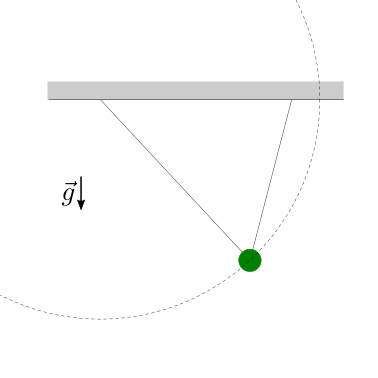
\includegraphics[width=.95\textwidth]{../../media/pb-statics-000-ese-000.png}
\end{minipage}
\end{split}
\end{equation*}
\sphinxAtStartPar
\sphinxstylestrong{Soluzione.}
I fili inestensibili senza massa e senza rigidezza flessionale possono solo trasmettere un’azione assiale. Ci si aiuta qui con un sistema di coordinate cartesiane con asse \(x\) orizzontale con coordinata crescente verso destra e asse \(y\) verticale con coordinata crescente verso l’alto. Date le direzioni dei fili identificate dai vettori unitari \(\hat{t}_1\), \(\hat{t}_2\), l’equilibrio della massa \(m\) è garantito dall’equilibrio delle forze,
\begin{equation*}
\begin{split}\hat{0} = -m g \hat{y} + F_1 \hat{t}_1 + F_2 \hat{t}_2 \ .\end{split}
\end{equation*}
\sphinxAtStartPar
Definiti gli angoli \(\theta_1\), \(\theta_2\), calcolabili dalla geometria del problema \sphinxhyphen{} qui considerati noti e calcolati in seguito \sphinxhyphen{} e tali che \(\hat{t}_1 = \hat{x} \cos \theta_1 + \hat{y}  \sin \theta_1\), \(\hat{t}_2 = \hat{x} \cos \theta_2 + \hat{y} \sin \theta_2\), le componenti cartesiane della condizione di equilibrio forniscono un sistema di due equazioni nelle due incognite \(F_1\), \(F_2\),
\begin{equation*}
\begin{split}\begin{cases} 
  F_1 \cos \theta_1 + F_2 \cos \theta_2 = 0 \\
  F_1 \sin \theta_1 + F_2 \sin \theta_2 = m g \\
\end{cases}\end{split}
\end{equation*}
\sphinxAtStartPar
che ha soluzione
\begin{equation*}
\begin{split}
  \begin{bmatrix} F_1 \\ F_2 \end{bmatrix} 
    = \frac{1}{\cos \theta_1 \sin \theta_2 - \sin \theta_1 \cos \theta_2}
    \begin{bmatrix} \sin \theta_2 & - \cos \theta_2 \\ -\sin \theta_1 & \cos \theta_1 \end{bmatrix} \begin{bmatrix} 0 \\ m g \end{bmatrix} 
    = \frac{1}{\sin(\theta_2 - \theta_1)} \begin{bmatrix} - \cos \theta_2 \\ \cos \theta_1 \end{bmatrix} m g  \ .
\end{split}
\end{equation*}
\sphinxAtStartPar
\sphinxstylestrong{todo} \sphinxstyleemphasis{Controllare conti. Aggiungere immagine.}

\sphinxAtStartPar
\sphinxstylestrong{Grandezze geometriche del problema.} \sphinxstylestrong{todo}
\begin{equation*}
\begin{split}
\begin{minipage}[t]{.55\textwidth}
  \vspace{0pt}
  \textbf{Problema 2.}
  Data la massa $m$ della massa puntiforme appeso tramite due fili inestensibili ideali di lunghezza $L_1$ nota e $L_2$ variabile, si calcolino le reazioni a terra in funzione della lunghezza del filo $2$.
\end{minipage}
\hspace{.05\textwidth}
\begin{minipage}[t]{.40\textwidth}
  \vspace{0pt}
  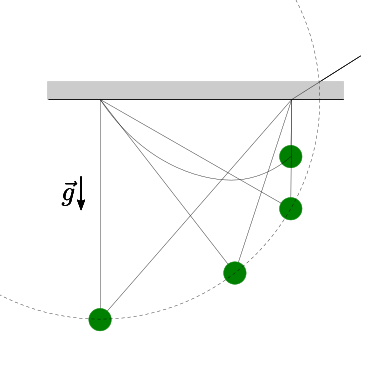
\includegraphics[width=.95\textwidth]{../../media/pb-statics-000-ese-001.png}
\end{minipage}
\end{split}
\end{equation*}
\sphinxAtStartPar
\sphinxstylestrong{Soluzione.}
\begin{equation*}
\begin{split}
\begin{minipage}[t]{.55\textwidth}
  \vspace{0pt}
  \textbf{Problema 3.}
  Data la massa $m$ della massa puntiforme appeso tramite un filo inestensibile ideale di lunghezza $L$ e una molla di costante elastica $k$ e lunghezza a riposo $x_0$ collegata a terra in un punto distante $H$ dal punto a terra dove è collegato il filo, si calcoli:
  \begin{enumerate}
    \item la posizione del punto 
    \item la lunghezza della molla
    \item le reazioni vincolari a terra 
  \end{enumerate}
  nella configurazione di equilibrio.
\end{minipage}
\hspace{.05\textwidth}
\begin{minipage}[t]{.40\textwidth}
  \vspace{0pt}
  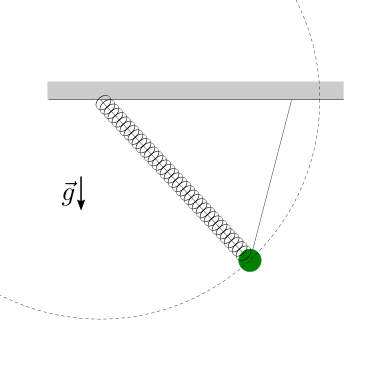
\includegraphics[width=.95\textwidth]{../../media/pb-statics-000-ese-002.png}
\end{minipage}
\end{split}
\end{equation*}
\sphinxAtStartPar
\sphinxstylestrong{Soluzione.}
\begin{equation*}
\begin{split}
\begin{minipage}[t]{.55\textwidth}
  \vspace{0pt}
  \textbf{Problema 4.}
  Data $m$, $\mu^s$, trovare l'angolo massimo $\theta_{\max}$ per il quale esiste una condizione di equilibrio per il cubetto rosso.
\end{minipage}
\hspace{.05\textwidth}
\begin{minipage}[t]{.40\textwidth}
  \vspace{0pt}
  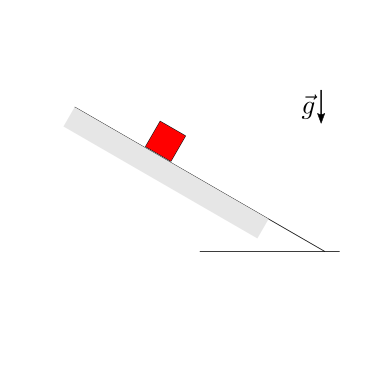
\includegraphics[width=.95\textwidth]{../../media/pb-statics-001-ese-000.png}
\end{minipage}
\end{split}
\end{equation*}
\sphinxAtStartPar
\sphinxstylestrong{Soluzione.}
Per l’equilibrio del corpo è necessario l’equilibrio delle forze. Le forze agenti sul cubetto rosso sono la sua forza peso e la reazione di contatto \(\vec{R}\) con la parete inclinata, che può essere scomposta nella direzione perpendicolare \sphinxhyphen{} reazione normale \sphinxhyphen{} e parallela alla parete \sphinxhyphen{} attrito.

\sphinxAtStartPar
La condizione di equilibrio,
\begin{equation*}
\begin{split}\vec{0} = -m g \hat{y} + \vec{R}\ ,\end{split}
\end{equation*}
\sphinxAtStartPar
può essere proiettata lungo la direzione normale alla parete \(\hat{n}\) e la direzione tangente \(\hat{t}\) (verto l’alto, così che \(\hat{y} = - \cos \theta \, \hat{n} - \sin \theta \, \hat{t}\)
\begin{equation*}
\begin{split}\begin{cases}
0 = N - m g \cos \theta \\
0 = F - m g \sin \theta \ ,
\end{cases}\end{split}
\end{equation*}
\sphinxAtStartPar
così che \(F = N \, \tan \theta\). Bisogna infine verificare che questa forza di attrito statico possa essere trasmessa, con la condizione
\begin{equation*}
\begin{split}|F| \le F^{s,max} = \mu^s \, N \ ,\end{split}
\end{equation*}
\sphinxAtStartPar
insieme alla condizione di contatto \(N \ge 0\), e quindi
\begin{equation*}
\begin{split}|\tan \theta| \le \mu^s \ .\end{split}
\end{equation*}\begin{equation*}
\begin{split}
\begin{minipage}[t]{.55\textwidth}
  \vspace{0pt}
  \textbf{Problema 5.}
  Data $m$, $M$, $\mu^s$ tra i due solidi, si chiede di calcolare:
  \begin{enumerate}
    \item la risultante delle azioni scambiate tra i due corpi
    \item la risultante delle reazioni vincolari a terra agenti sul solido blu,
  \end{enumerate}
  nella condizione di equilibrio del sistema, nell'ipotesi che l'attrito tra solido blu e terra sia trascurabile. Verificare le condizioni limite tra $\theta$ e $\mu^s$ affinché l'equilibrio sia possibile
\end{minipage}
\hspace{.05\textwidth}
\begin{minipage}[t]{.40\textwidth}
  \vspace{0pt}
  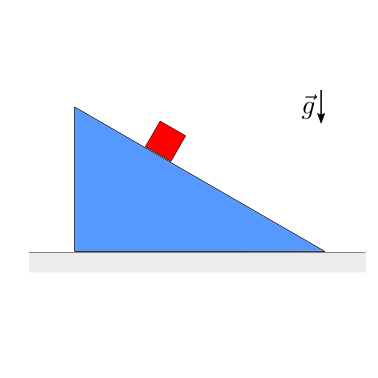
\includegraphics[width=.95\textwidth]{../../media/pb-statics-001-ese-001.png}
\end{minipage}
\end{split}
\end{equation*}
\sphinxAtStartPar
\sphinxstylestrong{Soluzione.}
Il piano orizzontale liscio non può trasmettere nessuna forza orizzontale al prisma triangolare. L’equilibrio delle forze del prisma triangolare, necessaria alla condizione di equilibrio, implica quindi che la risultante delle forze di contatto con il blocchetto rosso ha direzione verticale anch’essa.

\sphinxAtStartPar
Dalla condizione di equilibrio per il blocchetto rosso,
\begin{equation*}
\begin{split}\vec{0} = - m g \hat{y} + \vec{R}_{quad, tri} \qquad \rightarrow \qquad \vec{R}_{quad, tri} = m g \hat{y} \ .\end{split}
\end{equation*}
\sphinxAtStartPar
La risultante delle forze scambiate tra i corpi è quindi uguale e contraria al peso del cubetto (\sphinxstylestrong{1}). L’equilibrio del corpo triangolare
\begin{equation*}
\begin{split}
  \vec{0} = - M g \hat{y} + \vec{R}_{tri, quad} + \vec{R}_{tri, plane} \ ,
\end{split}
\end{equation*}
\sphinxAtStartPar
implica che la reazione \(\vec{R}_{tri,plane}\) agente sul solido triangolare dovuta alla superficie orizzontale è uguale e contraria alla somma del peso dei due solidi (\sphinxstylestrong{2}),
\begin{equation*}
\begin{split}
  \vec{R}_{tri,plane}   = M g \hat{y} - \vec{R}_{tri, quad}     
                        = M g \hat{y} + \vec{R}_{quad, tri}     
                        = M g \hat{y} + m g \hat{y} \ .
\end{split}
\end{equation*}\begin{equation*}
\begin{split}
\begin{minipage}[t]{.55\textwidth}
  \vspace{0pt}
  \textbf{Problema 6.}
  Data la massa $m$ del blocco rosso, la costante elastica $k$ della molla lineare ideale, con lunghezza a riposo $\ell_0$, viene chiesto di:
  \begin{enumerate}
    \item determinare la lunghezza della molla nella condizione di equilibrio, nell'ipotesi che l'attrito tra blocco rosso e piano inclinato sia trascurabile
    \item determinare le possibili condizioni di equilibrio, nell'ipotesi che l'attrito statico tra blocco rosso e piano inclinato sia $\mu^s$
  \end{enumerate}
\end{minipage}
\hspace{.05\textwidth}
\begin{minipage}[t]{.40\textwidth}
  \vspace{0pt}
  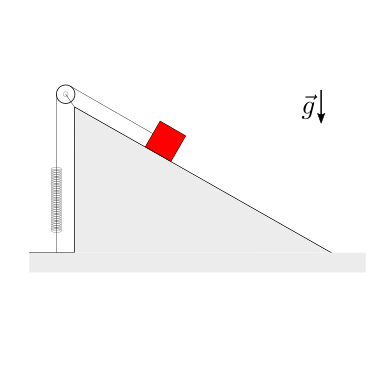
\includegraphics[width=.95\textwidth]{../../media/pb-statics-001-ese-002.png}
\end{minipage}
\end{split}
\end{equation*}
\sphinxAtStartPar
\sphinxstylestrong{Soluzione.}
I fili inestensibili trasmettono solo azione assiale nela direzione del filo, costante in ogni sua sezione. Le condizioni di equilibrio alla rotazione di una carrucola assicurano che sia costante l’azione assiale ai due capi di un filo parzialmente avvolto attorno alla carrucola, nel caso di attriti nulli (carrucola ideale).

\sphinxAtStartPar
Il problema può essere risolto scrivendo le condiizoni di equilibrio della molla,
\begin{equation*}
\begin{split}F = k (\ell - \ell_0)\end{split}
\end{equation*}
\sphinxAtStartPar
e del blocchetto rosso, proiettate in direzione perpendicolare e tangente alla superficie inclinata
\begin{equation*}
\begin{split}
  \vec{0} = \vec{F} + m \vec{g} + \vec{R}
  \qquad , \qquad
  \begin{cases}
    t: \ 0 = - F + m g \sin \theta + F_t \\
    n: \ 0 = \ \ - m g \cos \theta + F_n \\
  \end{cases}
  \end{split}
\end{equation*}
\sphinxAtStartPar
\sphinxstylestrong{In assenza di attrito, \(F_t = 0\).} In assenza di attrito, la reazione tangenziale è nulla \(F_t = 0\) e quindi
\begin{equation*}
\begin{split}\begin{aligned}
  F_n          & = m g \cos \theta \\
  F            & = m g \sin \theta \\
  \Delta \ell  & = \frac{m g}{k} \sin \theta \\
\end{aligned}\end{split}
\end{equation*}
\sphinxAtStartPar
\sphinxstylestrong{Con attrito statico.} In presenza di attrito statico, la soluzione non è unicamente determinata ma bisogna discutere le condizioni che garantiscono l’equilibrio, verificando la condizione \(|F_t| \le \mu^s F_n\). Le espressione delle componenti normali e tangenziali della reazione vincolare agente sul blocchetto,
\begin{equation*}
\begin{split}\begin{aligned}
  F_n & = m g \cos \theta \\
  F_t & = k \Delta \ell - m g \sin \theta
\end{aligned}\end{split}
\end{equation*}
\sphinxAtStartPar
permettono di scrivere la condizione che garantisce l’equilibrio come
\begin{equation*}
\begin{split}
 | k \Delta \ell - m g \sin \theta | \le \mu_s m g \cos \theta 
\end{split}
\end{equation*}
\sphinxAtStartPar
e quindi
\begin{equation*}
\begin{split}- \mu_s m g \cos \theta + mg \sin \theta \le k \Delta \ell \le  \mu_s m g \cos \theta + mg \sin \theta \ .\end{split}
\end{equation*}\begin{equation*}
\begin{split}
\begin{minipage}[t]{.55\textwidth}
  \vspace{0pt}
  \textbf{Problema 7.}
  Data la massa $m$ del blocco rosso, il raggio $R_1$, $R_2$ delle due carrucole, si chiede di determinare la forza $\vec{F}$ da applicare nella condizione di equilibrio, nell'ipotesi di fili inestensibili e carrucole ideali e senza massa.
  % 
  Si chiede poi di ripetere il calcolo nell'ipotesi in cui la massa delle carrucole non sia trascurabile, ma siano $M_1$ per la carrucola vincolata a terra, e $M_2$ per la carrucola non vincolata a terra.
\end{minipage}
\hspace{.05\textwidth}
\begin{minipage}[t]{.40\textwidth}
  \vspace{0pt}
  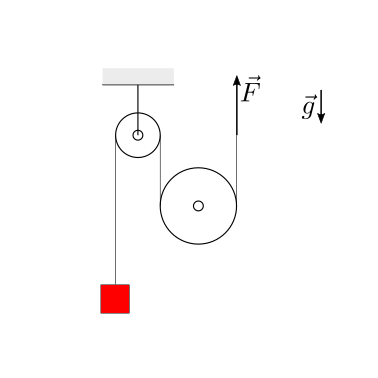
\includegraphics[width=.95\textwidth]{../../media/pb-statics-002-ese-000.png}
\end{minipage}
\end{split}
\end{equation*}
\sphinxAtStartPar
\sphinxstylestrong{Soluzione.}
\begin{equation*}
\begin{split}\begin{aligned}
0 & = - m g + T_1 \\
0 & = F + T_1 - M g \\
0 & - M g R_2 + F \, (2 R_2)
\end{aligned}\end{split}
\end{equation*}\begin{equation*}
\begin{split}\begin{aligned} 
  F & = \frac{1}{2} M g \\
  T_1
\end{aligned}
\end{split}
\end{equation*}\begin{equation*}
\begin{split}
\begin{minipage}[t]{.55\textwidth}
  \vspace{0pt}
  \textbf{Problema 8.}
  Nel meccanismo di un orologio i 3 componenti che devono guidare il moto delle lancette dei secondi, dei minuti e delle ore, connessi "in cascata" tramite ingranaggi (con rapporto dei raggi $1:60$ **todo** scriverlo esplicitamente?). Conoscendo la costante elastica $k$ e la compressione $\Delta \theta$ della molla che guida il componente che guida la lancetta delle ore, si chiede di:
  \begin{enumerate}
    \item determinare la forza necessaria da applicare alla lancetta dei secondi nel punto indicato nell'imagine, necessaria a garantire la posizione di equilibrio
    \item le reazioni vincolari in corrispondenza delle cerniere che collegano a terra i 3 componenti, nell'ipotesi che non si scambino forze in direzione radiale
  \end{enumerate}
\end{minipage}
\hspace{.05\textwidth}
\begin{minipage}[t]{.40\textwidth}
  \vspace{0pt}
  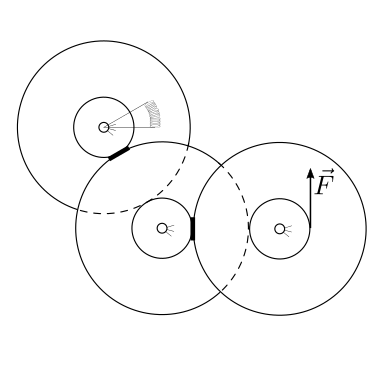
\includegraphics[width=.95\textwidth]{../../media/pb-statics-002-ese-001.png}
\end{minipage}
\end{split}
\end{equation*}
\sphinxAtStartPar
\sphinxstylestrong{Soluzione.}
\begin{equation*}
\begin{split}
F      R_1 & = F_{12} R_2 \\
F_{12} R_2 & = F_{23} R_3 \\
F_{23} R_3 & = k \Delta \theta \ .
\end{split}
\end{equation*}\begin{equation*}
\begin{split}
  F = \frac{R_2}{R_1} \frac{R_3}{R_2} \frac{1}{R_3} k \Delta \theta \ .
\end{split}
\end{equation*}\begin{equation*}
\begin{split}
\begin{minipage}[t]{.55\textwidth}
  \vspace{0pt}
  \textbf{Problema 9.}
  Data la lunghezza $L$ e la massa $m$ dell'asta rigida con distribuzione di massa uniforme e il coefficiente di attrito stativo $\mu^s$ tra asta e superficie orizzontale, si chiede di:
  \begin{enumerate}
    \item determinare la condizione limite dell'equilibrio
    \item determinare le reazioni a terra
  \end{enumerate}
  nell'ipotesi che l'attrito sulla superficie verticale sia trascurabile.
\end{minipage}
\hspace{.05\textwidth}
\begin{minipage}[t]{.40\textwidth}
  \vspace{0pt}
  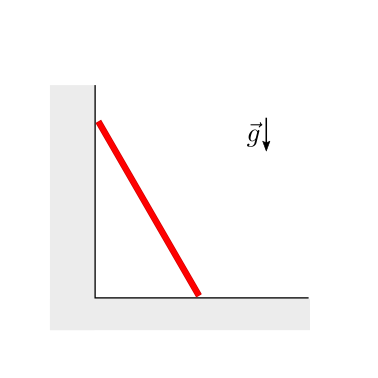
\includegraphics[width=.95\textwidth]{../../media/pb-statics-002-ese-002.png}
\end{minipage}
\end{split}
\end{equation*}
\sphinxAtStartPar
\sphinxstylestrong{Soluzione.}
\begin{equation*}
\begin{split}\begin{aligned}
x & : 0 =  N_{1} + F^{s}_2 \\
y & : 0 = - m g + N_{2} \\
\text{rot, 2} & : 0 = m g \frac{\ell}{2} \cos \theta - N_{1} \ell \sin \theta
\end{aligned}\end{split}
\end{equation*}\begin{equation*}
\begin{split}
\begin{minipage}[t]{.55\textwidth}
  \vspace{0pt}
  \textbf{Problema 10.}
  Data la lunghezza $L$ e la massa $m$ dell'asta rigida incernierata a terra, e la costante elastica $k$ della molla rotazionale, si chiede di:
  \begin{enumerate}
    \item calcolare la condizione di equilibrio
    \item le reazioni vincolari sull'asta
  \end{enumerate}
  discutendo i due casi determinati dalla condizione di appoggio dell'estremo superiore dell'asta sulla parete verticale.
\end{minipage}
\hspace{.05\textwidth}
\begin{minipage}[t]{.40\textwidth}
  \vspace{0pt}
  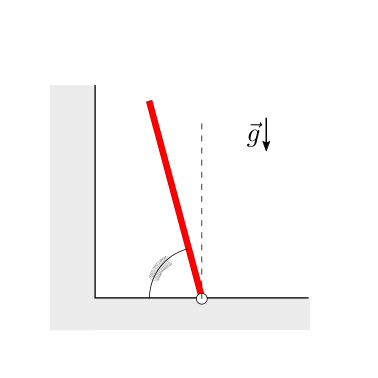
\includegraphics[width=.95\textwidth]{../../media/pb-statics-002-ese-003.png}
\end{minipage}
\end{split}
\end{equation*}
\sphinxAtStartPar
\sphinxstylestrong{Soluzione.}
Nel caso generale,
\begin{equation*}
\begin{split}\begin{aligned}
  x & : 0 =  N_{1} + F_{2,x} \\
  y & : 0 =  - m g + F_{2,y} \\
  \text{rot, 2} & : 0 = m g \frac{\ell}{2} \cos \theta - N_{1} \ell \sin \theta + k \Delta \theta
\end{aligned}\end{split}
\end{equation*}
\sphinxAtStartPar
Il contatto avviene quando la rigidezza della molla garantisce una condizione di equilibrio con \(\Delta \theta < \overline{\Delta \theta}\).
Se non c’è contatto, \(N_1 = 0\); se c’è contatto, in generale \(N_1 > 0\).
\begin{equation*}
\begin{split}
\begin{minipage}[t]{.55\textwidth}
  \vspace{0pt}
  \textbf{Problema 11.}
\end{minipage}
\hspace{.05\textwidth}
\begin{minipage}[t]{.40\textwidth}
  \vspace{0pt}
  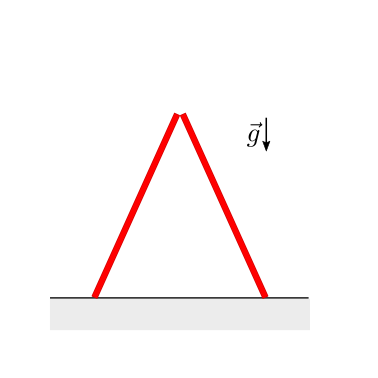
\includegraphics[width=.95\textwidth]{../../media/pb-statics-002-ese-004.png}
\end{minipage}
\end{split}
\end{equation*}
\sphinxAtStartPar
\sphinxstylestrong{Soluzione.}
\begin{equation*}
\begin{split}
\begin{minipage}[t]{.55\textwidth}
  \vspace{0pt}
  \textbf{Problema 12.}
\end{minipage}
\hspace{.05\textwidth}
\begin{minipage}[t]{.40\textwidth}
  \vspace{0pt}
  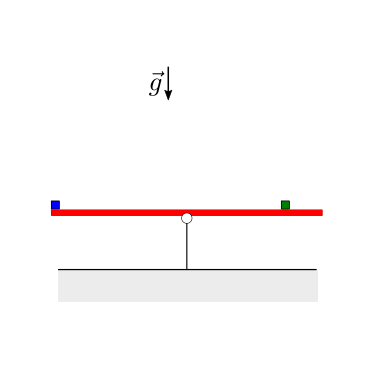
\includegraphics[width=.95\textwidth]{../../media/pb-statics-002-ese-005.png}
\end{minipage}
\end{split}
\end{equation*}
\sphinxAtStartPar
\sphinxstylestrong{Soluzione.}
\begin{equation*}
\begin{split}
\begin{minipage}[t]{.55\textwidth}
  \vspace{0pt}
  \textbf{Problema 13.}
\end{minipage}
\hspace{.05\textwidth}
\begin{minipage}[t]{.40\textwidth}
  \vspace{0pt}
  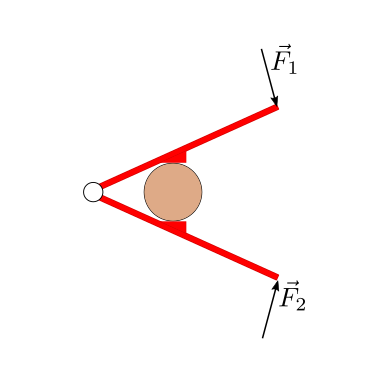
\includegraphics[width=.95\textwidth]{../../media/pb-statics-002-ese-006.png}
\end{minipage}
\end{split}
\end{equation*}
\sphinxAtStartPar
\sphinxstylestrong{Soluzione.}
\begin{equation*}
\begin{split}
\begin{minipage}[t]{.55\textwidth}
  \vspace{0pt}
  \textbf{Problema 14.}
\end{minipage}
\hspace{.05\textwidth}
\begin{minipage}[t]{.40\textwidth}
  \vspace{0pt}
  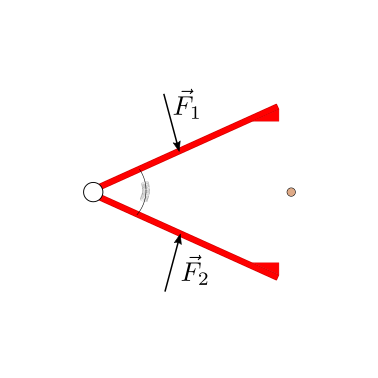
\includegraphics[width=.95\textwidth]{../../media/pb-statics-002-ese-007.png}
\end{minipage}
\end{split}
\end{equation*}
\sphinxAtStartPar
\sphinxstylestrong{Soluzione.}
\begin{equation*}
\begin{split}
\begin{minipage}[t]{.55\textwidth}
  \vspace{0pt}
  \textbf{Problema 15.}
  Equilibrio di un corpo appoggiato...esempio che mostra come la retta di applicazione del peso deve cadere nella base di appoggio; qui non è possibile introdurre l'accelerazione del sistema (**todo** *aggiungere esercizio nel capitolo della dinamica*), ma si può fare un esercizio con superficie di appoggio permendicolare e non al campo di gravità locale. L'unica cosa che conta è la direzione relativa tra superficie di appoggio e forza di massa. Rimandare all'esercizio sulla dinamica con collegamento
\end{minipage}
\hspace{.05\textwidth}
\begin{minipage}[t]{.40\textwidth}
\end{minipage}
\end{split}
\end{equation*}
\sphinxAtStartPar
\sphinxstylestrong{Soluzione.}
\begin{equation*}
\begin{split}
\begin{minipage}[t]{.55\textwidth}
  \vspace{0pt}
  \textbf{Problema 16.}
  Sollevamento di un peso sbilanciato, come mostrato in un *"video virale"*
\end{minipage}
\hspace{.05\textwidth}
\begin{minipage}[t]{.40\textwidth}
\end{minipage}
\end{split}
\end{equation*}
\sphinxAtStartPar
\sphinxstylestrong{Soluzione.}

\sphinxstepscope

\begin{sphinxuseclass}{sd-container-fluid}
\begin{sphinxuseclass}{sd-sphinx-override}
\begin{sphinxuseclass}{sd-p-0}
\begin{sphinxuseclass}{sd-mt-2}
\begin{sphinxuseclass}{sd-mb-4}
\begin{sphinxuseclass}{sd-row}
\begin{sphinxuseclass}{sd-row-cols-2}
\begin{sphinxuseclass}{sd-gx-2}
\begin{sphinxuseclass}{sd-gy-1}
\begin{sphinxuseclass}{sd-col}
\begin{sphinxuseclass}{sd-d-flex-row}
\begin{sphinxuseclass}{sd-align-minor-center}
\begin{sphinxuseclass}{sd-container-fluid}
\begin{sphinxuseclass}{sd-sphinx-override}
\begin{sphinxuseclass}{sd-row}
\begin{sphinxuseclass}{sd-row-cols-2}
\begin{sphinxuseclass}{sd-row-cols-xs-2}
\begin{sphinxuseclass}{sd-row-cols-sm-3}
\begin{sphinxuseclass}{sd-row-cols-md-3}
\begin{sphinxuseclass}{sd-row-cols-lg-3}
\begin{sphinxuseclass}{sd-gx-3}
\begin{sphinxuseclass}{sd-gy-1}
\begin{sphinxuseclass}{sd-col}
\begin{sphinxuseclass}{sd-col-auto}
\begin{sphinxuseclass}{sd-d-flex-row}
\begin{sphinxuseclass}{sd-align-minor-center}
\sphinxAtStartPar
basics

\end{sphinxuseclass}
\end{sphinxuseclass}
\end{sphinxuseclass}
\end{sphinxuseclass}
\begin{sphinxuseclass}{sd-col}
\begin{sphinxuseclass}{sd-col-auto}
\begin{sphinxuseclass}{sd-d-flex-row}
\begin{sphinxuseclass}{sd-align-minor-center}
\sphinxAtStartPar
28 nov 2024

\end{sphinxuseclass}
\end{sphinxuseclass}
\end{sphinxuseclass}
\end{sphinxuseclass}
\begin{sphinxuseclass}{sd-col}
\begin{sphinxuseclass}{sd-col-auto}
\begin{sphinxuseclass}{sd-d-flex-row}
\begin{sphinxuseclass}{sd-align-minor-center}
\sphinxAtStartPar
1 min read

\end{sphinxuseclass}
\end{sphinxuseclass}
\end{sphinxuseclass}
\end{sphinxuseclass}
\end{sphinxuseclass}
\end{sphinxuseclass}
\end{sphinxuseclass}
\end{sphinxuseclass}
\end{sphinxuseclass}
\end{sphinxuseclass}
\end{sphinxuseclass}
\end{sphinxuseclass}
\end{sphinxuseclass}
\end{sphinxuseclass}
\end{sphinxuseclass}
\end{sphinxuseclass}
\end{sphinxuseclass}
\end{sphinxuseclass}
\end{sphinxuseclass}
\end{sphinxuseclass}
\end{sphinxuseclass}
\end{sphinxuseclass}
\end{sphinxuseclass}
\end{sphinxuseclass}
\end{sphinxuseclass}
\end{sphinxuseclass}

\chapter{Inerzia}
\label{\detokenize{ch/mechanics/inertia:inerzia}}\label{\detokenize{ch/mechanics/inertia:physics-hs-mechanics-inertia}}\label{\detokenize{ch/mechanics/inertia::doc}}

\section{Massa e distribuzione di massa}
\label{\detokenize{ch/mechanics/inertia:massa-e-distribuzione-di-massa}}
\sphinxAtStartPar
La massa è la grandezza fisica che rappresenta la quantità di materia (\sphinxstylestrong{todo} \sphinxstyleemphasis{Non confonderla con la mole, definita come quantità di sostanza, una volta affermatasi la teoria atomica})

\sphinxAtStartPar
In meccanica classica, la può essere definita in maniera operativa:
\begin{itemize}
\item {} 
\sphinxAtStartPar
tramite la sua {\hyperref[\detokenize{ch/mechanics/actions-examples:physics-hs-mechanics-actions-gravitation}]{\sphinxcrossref{\DUrole{std,std-ref}{interazione gravitazionale}}}} con altri corpi dotati di massa

\item {} 
\sphinxAtStartPar
come una misura della resistenza di un sistema ai cambiamenti del suo stato di moto in risposta a una forza applicata, come sarà chiaro dalle equazioni della {\hyperref[\detokenize{ch/mechanics/dynamics:physics-hs-mechanics-dynamics}]{\sphinxcrossref{\DUrole{std,std-ref}{dinamica}}}}

\end{itemize}


\section{Quantità dinamiche}
\label{\detokenize{ch/mechanics/inertia:quantita-dinamiche}}
\sphinxAtStartPar
Come sarà chiaro nello sviluppo delle {\hyperref[\detokenize{ch/mechanics/dynamics-eom-proof-points:physics-hs-mechanics-dynamics-eom-points}]{\sphinxcrossref{\DUrole{std,std-ref}{equazioni di moto di un sistema}}}}, la definizione di alcune grandezze dinamiche additive risulta naturale, fornendo dei concetti utili e sintetici per la costruzione di un modello e l’interpretazione dei fenomeni fisici.

\sphinxAtStartPar
Queste grandezze dinamiche combinano la massa e la sua distribuzione con le grandezze cinematiche del sistema. In particolare, risulta utile definire tre grandezze:
\begin{itemize}
\item {} 
\sphinxAtStartPar
quantità di moto

\item {} 
\sphinxAtStartPar
momento della quantità di moto

\item {} 
\sphinxAtStartPar
energia cinetica

\end{itemize}

\sphinxAtStartPar
Le {\hyperref[\detokenize{ch/mechanics/dynamics-eom:physics-hs-mechanics-dynamics-eom}]{\sphinxcrossref{\DUrole{std,std-ref}{equazioni del moto}}}} dei sistemi rappresentano delle equazioni differenziali che mettono in relazione la variazione di queste quantità dinamiche con la causa di queste variazioni, in generale riconducibile ad {\hyperref[\detokenize{ch/mechanics/actions:physics-hs-mechanics-actions}]{\sphinxcrossref{\DUrole{std,std-ref}{azioni}}}} agenti sul sistema.

\sphinxAtStartPar
Sotto opportune ipotesi, queste grandezze dinamiche sono costanti del moto, come descritto dalle {\hyperref[\detokenize{ch/mechanics/dynamics-conservation:physics-hs-mechanics-dynamics-conservation}]{\sphinxcrossref{\DUrole{std,std-ref}{leggi di conservazione}}}}.

\sphinxAtStartPar
Le 3 grandezze dinamiche possono avere espressioni diverse, a seconda del sistema di interesse. Nel caso di corpi rigidi, queste possono essere espresse in termini di velocità di un punto materiale e della velocità angolare del corpo.

\sphinxstepscope

\begin{sphinxuseclass}{sd-container-fluid}
\begin{sphinxuseclass}{sd-sphinx-override}
\begin{sphinxuseclass}{sd-p-0}
\begin{sphinxuseclass}{sd-mt-2}
\begin{sphinxuseclass}{sd-mb-4}
\begin{sphinxuseclass}{sd-row}
\begin{sphinxuseclass}{sd-row-cols-2}
\begin{sphinxuseclass}{sd-gx-2}
\begin{sphinxuseclass}{sd-gy-1}
\begin{sphinxuseclass}{sd-col}
\begin{sphinxuseclass}{sd-d-flex-row}
\begin{sphinxuseclass}{sd-align-minor-center}
\begin{sphinxuseclass}{sd-container-fluid}
\begin{sphinxuseclass}{sd-sphinx-override}
\begin{sphinxuseclass}{sd-row}
\begin{sphinxuseclass}{sd-row-cols-2}
\begin{sphinxuseclass}{sd-row-cols-xs-2}
\begin{sphinxuseclass}{sd-row-cols-sm-3}
\begin{sphinxuseclass}{sd-row-cols-md-3}
\begin{sphinxuseclass}{sd-row-cols-lg-3}
\begin{sphinxuseclass}{sd-gx-3}
\begin{sphinxuseclass}{sd-gy-1}
\begin{sphinxuseclass}{sd-col}
\begin{sphinxuseclass}{sd-col-auto}
\begin{sphinxuseclass}{sd-d-flex-row}
\begin{sphinxuseclass}{sd-align-minor-center}
\sphinxAtStartPar
basics

\end{sphinxuseclass}
\end{sphinxuseclass}
\end{sphinxuseclass}
\end{sphinxuseclass}
\begin{sphinxuseclass}{sd-col}
\begin{sphinxuseclass}{sd-col-auto}
\begin{sphinxuseclass}{sd-d-flex-row}
\begin{sphinxuseclass}{sd-align-minor-center}
\sphinxAtStartPar
28 nov 2024

\end{sphinxuseclass}
\end{sphinxuseclass}
\end{sphinxuseclass}
\end{sphinxuseclass}
\begin{sphinxuseclass}{sd-col}
\begin{sphinxuseclass}{sd-col-auto}
\begin{sphinxuseclass}{sd-d-flex-row}
\begin{sphinxuseclass}{sd-align-minor-center}
\sphinxAtStartPar
0 min read

\end{sphinxuseclass}
\end{sphinxuseclass}
\end{sphinxuseclass}
\end{sphinxuseclass}
\end{sphinxuseclass}
\end{sphinxuseclass}
\end{sphinxuseclass}
\end{sphinxuseclass}
\end{sphinxuseclass}
\end{sphinxuseclass}
\end{sphinxuseclass}
\end{sphinxuseclass}
\end{sphinxuseclass}
\end{sphinxuseclass}
\end{sphinxuseclass}
\end{sphinxuseclass}
\end{sphinxuseclass}
\end{sphinxuseclass}
\end{sphinxuseclass}
\end{sphinxuseclass}
\end{sphinxuseclass}
\end{sphinxuseclass}
\end{sphinxuseclass}
\end{sphinxuseclass}
\end{sphinxuseclass}
\end{sphinxuseclass}

\section{Inerzia e grandezze dinamiche di un punto}
\label{\detokenize{ch/mechanics/inertia-point:inerzia-e-grandezze-dinamiche-di-un-punto}}\label{\detokenize{ch/mechanics/inertia-point::doc}}\begin{equation*}
\begin{split}\begin{aligned}
  \vec{Q}_P     & = m_P \, \vec{v}_P \\
  \vec{L}_{P,H} & = m_P \, (P - H) \times \vec{v}_P \\
   K_P          & = \frac{1}{2} m_P \left| \vec{v}_P \right|^2
\end{aligned}\end{split}
\end{equation*}
\sphinxstepscope

\begin{sphinxuseclass}{sd-container-fluid}
\begin{sphinxuseclass}{sd-sphinx-override}
\begin{sphinxuseclass}{sd-p-0}
\begin{sphinxuseclass}{sd-mt-2}
\begin{sphinxuseclass}{sd-mb-4}
\begin{sphinxuseclass}{sd-row}
\begin{sphinxuseclass}{sd-row-cols-2}
\begin{sphinxuseclass}{sd-gx-2}
\begin{sphinxuseclass}{sd-gy-1}
\begin{sphinxuseclass}{sd-col}
\begin{sphinxuseclass}{sd-d-flex-row}
\begin{sphinxuseclass}{sd-align-minor-center}
\begin{sphinxuseclass}{sd-container-fluid}
\begin{sphinxuseclass}{sd-sphinx-override}
\begin{sphinxuseclass}{sd-row}
\begin{sphinxuseclass}{sd-row-cols-2}
\begin{sphinxuseclass}{sd-row-cols-xs-2}
\begin{sphinxuseclass}{sd-row-cols-sm-3}
\begin{sphinxuseclass}{sd-row-cols-md-3}
\begin{sphinxuseclass}{sd-row-cols-lg-3}
\begin{sphinxuseclass}{sd-gx-3}
\begin{sphinxuseclass}{sd-gy-1}
\begin{sphinxuseclass}{sd-col}
\begin{sphinxuseclass}{sd-col-auto}
\begin{sphinxuseclass}{sd-d-flex-row}
\begin{sphinxuseclass}{sd-align-minor-center}
\sphinxAtStartPar
basics

\end{sphinxuseclass}
\end{sphinxuseclass}
\end{sphinxuseclass}
\end{sphinxuseclass}
\begin{sphinxuseclass}{sd-col}
\begin{sphinxuseclass}{sd-col-auto}
\begin{sphinxuseclass}{sd-d-flex-row}
\begin{sphinxuseclass}{sd-align-minor-center}
\sphinxAtStartPar
28 nov 2024

\end{sphinxuseclass}
\end{sphinxuseclass}
\end{sphinxuseclass}
\end{sphinxuseclass}
\begin{sphinxuseclass}{sd-col}
\begin{sphinxuseclass}{sd-col-auto}
\begin{sphinxuseclass}{sd-d-flex-row}
\begin{sphinxuseclass}{sd-align-minor-center}
\sphinxAtStartPar
0 min read

\end{sphinxuseclass}
\end{sphinxuseclass}
\end{sphinxuseclass}
\end{sphinxuseclass}
\end{sphinxuseclass}
\end{sphinxuseclass}
\end{sphinxuseclass}
\end{sphinxuseclass}
\end{sphinxuseclass}
\end{sphinxuseclass}
\end{sphinxuseclass}
\end{sphinxuseclass}
\end{sphinxuseclass}
\end{sphinxuseclass}
\end{sphinxuseclass}
\end{sphinxuseclass}
\end{sphinxuseclass}
\end{sphinxuseclass}
\end{sphinxuseclass}
\end{sphinxuseclass}
\end{sphinxuseclass}
\end{sphinxuseclass}
\end{sphinxuseclass}
\end{sphinxuseclass}
\end{sphinxuseclass}
\end{sphinxuseclass}

\section{Inerzia e grandezze dinamiche di un sistema esteso con distribuzione discreta di massa}
\label{\detokenize{ch/mechanics/inertia-points:inerzia-e-grandezze-dinamiche-di-un-sistema-esteso-con-distribuzione-discreta-di-massa}}\label{\detokenize{ch/mechanics/inertia-points::doc}}\begin{equation*}
\begin{split}\begin{aligned}
  \vec{Q}       = \sum_i \vec{Q}_i     & = \sum_i  m_i \, \vec{v}_i \\
  \vec{L}_{H}   = \sum_i \vec{L}_{i,H} & = \sum_i  m_i \, (P_i - H) \times \vec{v}_i \\
   K            = \sum_i  K_i          & = \sum_i  \frac{1}{2} m_i \left| \vec{v}_i \right|^2
\end{aligned}\end{split}
\end{equation*}

\subsection{Sistemi rigidi}
\label{\detokenize{ch/mechanics/inertia-points:sistemi-rigidi}}
\sphinxAtStartPar
Usando la definizione di centro di massa
\begin{equation*}
\begin{split}m G = \sum_i m_i P_i\end{split}
\end{equation*}
\sphinxAtStartPar
e legge del moto rigido
\begin{equation*}
\begin{split}\vec{v}_i - \vec{v}_P = \vec{\omega} \times (P_i - P)\end{split}
\end{equation*}
\sphinxAtStartPar
le quantità dinamiche possono essere espresse in funzione della velocità del punto di riferimento \(P\) e della velocità angolare del sistema, tramite la massa e le altre quantità inerziali
\begin{itemize}
\item {} 
\sphinxAtStartPar
la quantità di moto

\end{itemize}
\begin{equation*}
\begin{split}\begin{aligned}
  \vec{Q} = \sum_i m_i \vec{v}_i
        & = \sum_i m_i \left( \vec{v}_P + \vec{\omega} \times (P_i - P) \right) = \\
        & =  m \vec{v}_P + \vec{\omega} \times m (G - P) 
\end{aligned}\end{split}
\end{equation*}\begin{itemize}
\item {} 
\sphinxAtStartPar
momento della quantità di moto

\end{itemize}
\begin{equation*}
\begin{split}\begin{aligned}
  \vec{L}_H = \sum_i m_i (P_i - H) \times \vec{v}_i
        & = \sum_i m_i \left( P_i - P + \vec{r}_P - \vec{r}_H \right) \times \vec{v}_i = \\
        & = \sum_i m_i \left( P_i - P \right) \times \vec{v}_i + \left( P - H \right) \times \vec{Q}  = \\
        & = \sum_i m_i \left( P_i - P \right) \times \left( \vec{v}_P - \left( P_i - P \right) \times \vec{\omega} \right) + \left( P - H \right) \times \vec{Q}  = \\
        & = m (G - P) \times \vec{v}_P - \sum_i m_i \left( P_i - P \right) \times \left( \left( P_i - P \right) \times \vec{\omega} \right) + \left( P - H \right) \times \vec{Q}  = \\
        & = \mathbb{I}_P \cdot \vec{\omega} +  m (G - P) \times \vec{v}_P + \left( P - H \right) \times \vec{Q}
\end{aligned}\end{split}
\end{equation*}
\sphinxAtStartPar
Nel caso di moto 2\sphinxhyphen{}dimensionale e velocità angolare perpendicolare a questo piano, \sphinxstylestrong{todo}
\begin{equation*}
\begin{split}\begin{aligned}
  \vec{r}_{i/P} & := P_i - P = \left( x_i - x_P \right) \hat{x} + \left( y_i - y_P \right) \hat{y} \\
  \vec{\omega} & = \dot{\theta} \, \hat{z}
\end{aligned}\end{split}
\end{equation*}\begin{equation*}
\begin{split}\begin{aligned}
  - \vec{r}_{i/P} \times \left( \vec{r}_{i/P} \times \hat{\omega} \right) 
  & = - ( \Delta x_i \hat{x} + \Delta y_i \hat{y} ) \times \left[ ( \Delta x_i \hat{x} + \Delta y_i \hat{y} ) \times \dot{\theta} \hat{z} \right] = \\ 
  & = - \dot{\theta} ( \Delta x_i \hat{x} + \Delta y_i \hat{y} ) \times \left( - \Delta x_i \hat{y} + \Delta y_i \hat{x} \right) = \\
  & = \left( \Delta x_i^2 + \Delta y_i^2 \right) \dot{\theta} \, \hat{z} \ .
\end{aligned}\end{split}
\end{equation*}
\sphinxAtStartPar
e l’espressione del momento della quantità di moto diventa
\begin{equation*}
\begin{split}\vec{L}_{H} = I_P \, \vec{\omega} +  m (G - P) \times \vec{v}_P + \left( P - H \right) \times \vec{Q}\end{split}
\end{equation*}
\sphinxAtStartPar
con
\begin{equation*}
\begin{split}I_P = \sum_i m_i \left[ \left(x_i - x_P\right)^2 + \left(y_i - y_P\right)^2 \right]\end{split}
\end{equation*}
\sphinxstepscope

\begin{sphinxuseclass}{sd-container-fluid}
\begin{sphinxuseclass}{sd-sphinx-override}
\begin{sphinxuseclass}{sd-p-0}
\begin{sphinxuseclass}{sd-mt-2}
\begin{sphinxuseclass}{sd-mb-4}
\begin{sphinxuseclass}{sd-row}
\begin{sphinxuseclass}{sd-row-cols-2}
\begin{sphinxuseclass}{sd-gx-2}
\begin{sphinxuseclass}{sd-gy-1}
\begin{sphinxuseclass}{sd-col}
\begin{sphinxuseclass}{sd-d-flex-row}
\begin{sphinxuseclass}{sd-align-minor-center}
\begin{sphinxuseclass}{sd-container-fluid}
\begin{sphinxuseclass}{sd-sphinx-override}
\begin{sphinxuseclass}{sd-row}
\begin{sphinxuseclass}{sd-row-cols-2}
\begin{sphinxuseclass}{sd-row-cols-xs-2}
\begin{sphinxuseclass}{sd-row-cols-sm-3}
\begin{sphinxuseclass}{sd-row-cols-md-3}
\begin{sphinxuseclass}{sd-row-cols-lg-3}
\begin{sphinxuseclass}{sd-gx-3}
\begin{sphinxuseclass}{sd-gy-1}
\begin{sphinxuseclass}{sd-col}
\begin{sphinxuseclass}{sd-col-auto}
\begin{sphinxuseclass}{sd-d-flex-row}
\begin{sphinxuseclass}{sd-align-minor-center}
\sphinxAtStartPar
basics

\end{sphinxuseclass}
\end{sphinxuseclass}
\end{sphinxuseclass}
\end{sphinxuseclass}
\begin{sphinxuseclass}{sd-col}
\begin{sphinxuseclass}{sd-col-auto}
\begin{sphinxuseclass}{sd-d-flex-row}
\begin{sphinxuseclass}{sd-align-minor-center}
\sphinxAtStartPar
28 nov 2024

\end{sphinxuseclass}
\end{sphinxuseclass}
\end{sphinxuseclass}
\end{sphinxuseclass}
\begin{sphinxuseclass}{sd-col}
\begin{sphinxuseclass}{sd-col-auto}
\begin{sphinxuseclass}{sd-d-flex-row}
\begin{sphinxuseclass}{sd-align-minor-center}
\sphinxAtStartPar
0 min read

\end{sphinxuseclass}
\end{sphinxuseclass}
\end{sphinxuseclass}
\end{sphinxuseclass}
\end{sphinxuseclass}
\end{sphinxuseclass}
\end{sphinxuseclass}
\end{sphinxuseclass}
\end{sphinxuseclass}
\end{sphinxuseclass}
\end{sphinxuseclass}
\end{sphinxuseclass}
\end{sphinxuseclass}
\end{sphinxuseclass}
\end{sphinxuseclass}
\end{sphinxuseclass}
\end{sphinxuseclass}
\end{sphinxuseclass}
\end{sphinxuseclass}
\end{sphinxuseclass}
\end{sphinxuseclass}
\end{sphinxuseclass}
\end{sphinxuseclass}
\end{sphinxuseclass}
\end{sphinxuseclass}
\end{sphinxuseclass}

\section{Inerzia e grandezze dinamiche di un sistema esteso con distribuzione continua di massa}
\label{\detokenize{ch/mechanics/inertia-continuum:inerzia-e-grandezze-dinamiche-di-un-sistema-esteso-con-distribuzione-continua-di-massa}}\label{\detokenize{ch/mechanics/inertia-continuum::doc}}

\subsection{Sistemi rigidi}
\label{\detokenize{ch/mechanics/inertia-continuum:sistemi-rigidi}}
\sphinxstepscope

\begin{sphinxuseclass}{sd-container-fluid}
\begin{sphinxuseclass}{sd-sphinx-override}
\begin{sphinxuseclass}{sd-p-0}
\begin{sphinxuseclass}{sd-mt-2}
\begin{sphinxuseclass}{sd-mb-4}
\begin{sphinxuseclass}{sd-row}
\begin{sphinxuseclass}{sd-row-cols-2}
\begin{sphinxuseclass}{sd-gx-2}
\begin{sphinxuseclass}{sd-gy-1}
\begin{sphinxuseclass}{sd-col}
\begin{sphinxuseclass}{sd-d-flex-row}
\begin{sphinxuseclass}{sd-align-minor-center}
\begin{sphinxuseclass}{sd-container-fluid}
\begin{sphinxuseclass}{sd-sphinx-override}
\begin{sphinxuseclass}{sd-row}
\begin{sphinxuseclass}{sd-row-cols-2}
\begin{sphinxuseclass}{sd-row-cols-xs-2}
\begin{sphinxuseclass}{sd-row-cols-sm-3}
\begin{sphinxuseclass}{sd-row-cols-md-3}
\begin{sphinxuseclass}{sd-row-cols-lg-3}
\begin{sphinxuseclass}{sd-gx-3}
\begin{sphinxuseclass}{sd-gy-1}
\begin{sphinxuseclass}{sd-col}
\begin{sphinxuseclass}{sd-col-auto}
\begin{sphinxuseclass}{sd-d-flex-row}
\begin{sphinxuseclass}{sd-align-minor-center}
\sphinxAtStartPar
basics

\end{sphinxuseclass}
\end{sphinxuseclass}
\end{sphinxuseclass}
\end{sphinxuseclass}
\begin{sphinxuseclass}{sd-col}
\begin{sphinxuseclass}{sd-col-auto}
\begin{sphinxuseclass}{sd-d-flex-row}
\begin{sphinxuseclass}{sd-align-minor-center}
\sphinxAtStartPar
28 nov 2024

\end{sphinxuseclass}
\end{sphinxuseclass}
\end{sphinxuseclass}
\end{sphinxuseclass}
\begin{sphinxuseclass}{sd-col}
\begin{sphinxuseclass}{sd-col-auto}
\begin{sphinxuseclass}{sd-d-flex-row}
\begin{sphinxuseclass}{sd-align-minor-center}
\sphinxAtStartPar
1 min read

\end{sphinxuseclass}
\end{sphinxuseclass}
\end{sphinxuseclass}
\end{sphinxuseclass}
\end{sphinxuseclass}
\end{sphinxuseclass}
\end{sphinxuseclass}
\end{sphinxuseclass}
\end{sphinxuseclass}
\end{sphinxuseclass}
\end{sphinxuseclass}
\end{sphinxuseclass}
\end{sphinxuseclass}
\end{sphinxuseclass}
\end{sphinxuseclass}
\end{sphinxuseclass}
\end{sphinxuseclass}
\end{sphinxuseclass}
\end{sphinxuseclass}
\end{sphinxuseclass}
\end{sphinxuseclass}
\end{sphinxuseclass}
\end{sphinxuseclass}
\end{sphinxuseclass}
\end{sphinxuseclass}
\end{sphinxuseclass}

\chapter{Dinamica}
\label{\detokenize{ch/mechanics/dynamics:dinamica}}\label{\detokenize{ch/mechanics/dynamics:physics-hs-mechanics-dynamics}}\label{\detokenize{ch/mechanics/dynamics::doc}}
\sphinxAtStartPar
La dinamica si occupa del moto dei sistemi e delle cause del moto, mettendo insieme la descrizione cinematica, l’inerzia dei sistemi a perseverare nel moto, e le cause di una variazione del moto.

\sphinxAtStartPar
\sphinxstylestrong{Princìpi della dinamica.} Vengono discussi i tre principi della dinamica di Newton e il significato della relatività galileiana.

\sphinxAtStartPar
\sphinxstylestrong{Equazioni cardinali della dinamica.} Vengono presentate le tre equazioni cardinali della dinamica per sistemi chiusi, che mettono in relazione la variazione delle grandezze dinamiche alle azioni, e che nel caso di moti regolari possono essere scritte in forma differenziale
\begin{equation*}
\begin{split}\begin{aligned}
 \dot{\vec{Q}} & = \vec{R}^{ext} & \text{(bilancio quantità di moto)} \\
 \dot{\vec{L}}_H + \dot{\vec{x}}_H \times \vec{Q} & = \vec{M}_H^{ext} & \text{(bilancio momento della quantità di moto)} \\
 \dot{K} & = P^{tot} & \text{(bilancio energia cinetica)} \ .
\end{aligned}\end{split}
\end{equation*}
\sphinxAtStartPar
Viene dimostrato che le equazioni di bilancio hanno la stessa forma per ogni sistema chiuso se scritti in termini di variazione di quantità di moto, momento della quantità di moto ed energia cinetica, senza esplicitare la forma particolare di queste grandezze dinamiche per i sistemi particolari presi in considerazione. Vengono forniti alcuni esempi ed esercizi svolti.

\sphinxAtStartPar
\sphinxstylestrong{Leggi di conservazione.} Sotto opportune ipotesi immediatamente riconoscibili dalle equazioni cardinali, vengono ricavate le leggi di conservazione validi per i sistemi meccanici,
\begin{equation*}
\begin{split}\begin{aligned}
  \vec{R}^{ext} & = \vec{0} \qquad  & \rightarrow \qquad \ \ \vec{Q} = \text{const.} \\
  \vec{M}_H^{ext} & = \vec{0}, \dot{\vec{x}}_H \times \vec{Q} = \vec{0} \qquad  & \rightarrow \qquad \vec{L}_H = \text{const.} \\
  P^{tot} & = \vec{0} \qquad  & \rightarrow \qquad \ \  K = \text{const.} \\
\end{aligned}\end{split}
\end{equation*}
\sphinxAtStartPar
Nel caso in cui le azioni agenti sul sistema non abbiano potenza nulla, ma che siano forze conservative, si riconosce la legge di conservazione dell’energia meccanica \(E^{mec}\), definita come somma dell’energia cinetica, \(K\), e dell’energia potenziale, \(V\),
\begin{equation*}
\begin{split}P^{tot} = -\dot{V} \ , \quad E^{mec} = K + V \qquad \rightarrow \qquad E^{mec} = \text{const.}\end{split}
\end{equation*}
\sphinxAtStartPar
\sphinxstylestrong{Urti.}
Viene presentato un modello di urto tra sistemi fondato unicamente sul coefficiente di restituzione, \(\varepsilon\), per rappresentare la frazione di energia meccanica persa dal sistema durante l’urto. Vengono presentati dei problemi risolti grazie ai princìpi di conservazione e alle equazioni cardinali in forma incrementale.

\sphinxAtStartPar
\sphinxstylestrong{Moti particolari \sphinxhyphen{} gravitazione.} Vengono infine analizzati alcuni sistemi particolare, di interesse pratico, storico, e/o didattico \sphinxstylestrong{todo}



\sphinxstepscope


\section{Princìpi della dinamica di Newton}
\label{\detokenize{ch/mechanics/dynamics-principles:principi-della-dinamica-di-newton}}\label{\detokenize{ch/mechanics/dynamics-principles:physics-hs-mechanics-dynamics-principles}}\label{\detokenize{ch/mechanics/dynamics-principles::doc}}
\sphinxAtStartPar
La meccanica classica di Newton viene costruita assumendo valido il \sphinxstylestrong{principio di conservazione della massa} e i \sphinxstylestrong{tre principi della dinamica}.

\sphinxAtStartPar
\sphinxstylestrong{Principio di conservazione della massa.} In meccanica classica, il principio di Lavoisier di conservazione della massa può essere riassunto con la formula «niente si crea, niente si distrugge». Per essere più precisi, il principio di conservazione della massa postula che la massa di un sistema chiuso è costante.

\sphinxAtStartPar
\sphinxstylestrong{Primo principio \sphinxhyphen{} principio di inerzia.} Un sistema (o meglio, il baricentro di un sistema) sul quale agisce una forza esterna netta nulla, persevera nel suo stato di quiete o di moto rettilineo uniforme rispetto a un sistema di riferimento inerziale.

\sphinxAtStartPar
\sphinxstylestrong{Secondo principio \sphinxhyphen{} bilancio della quantità di moto per sistemi chiusi.} Rispetto a un sistema di riferimento inerziale, la variazione della quantità di moto \(\vec{Q}\) di un sistema chiuso è uguale all’impulso delle forze esterne \(\vec{I}^{ext}\) agenti su di esso,
\begin{equation*}
\begin{split}\Delta \vec{Q} = \vec{I}^{ext} \ .\end{split}
\end{equation*}
\sphinxAtStartPar
Nel caso di moto regolare, in cui la quantità di moto del sistema è una grandezza continua e differenziabile rispetto al tempo, il secondo principio può essere scritto in forma differenziale, facendo tendere a zero l’intervallo di tempo considerato
\begin{equation*}
\begin{split}\dot{\vec{Q}} = \vec{R}^{ext} \ ,\end{split}
\end{equation*}
\sphinxAtStartPar
avendo indicato con \(\vec{R}^{ext}\) la risultante delle forze esterne agenti sul sistema.

\sphinxAtStartPar
\sphinxstylestrong{Terzo principio \sphinxhyphen{} principio di azione\sphinxhyphen{}reazione.} Se un sistema \(i\) esercita una forza \(\vec{F}_{ji}\) sul sistema \(j\), allora il sistema \(j\) esercita sul sistema \(i\) una forza \(\vec{F}_{ij}\) «uguale e contraria» \sphinxhyphen{} stesso valore assoluto e verso opposto,
\begin{equation*}
\begin{split}\vec{F}_{ij} = - \vec{F}_{ji} \ .\end{split}
\end{equation*}
\sphinxAtStartPar
\sphinxstylestrong{todo} \sphinxstylestrong{Osservazioni}
\begin{itemize}
\item {} 
\sphinxAtStartPar
sistema di riferimento inerziale e invarianza galileiana

\item {} 
\sphinxAtStartPar
sistemi aperti e sistemi chiusi: sottolineare la validità di \(\Delta \vec{Q} = \vec{I}^{ext}\) solo per sistemi chiusi, mentre per sistemi aperti è necessario un termine di flusso della quantità meccanica. Riferimento alla meccanica dei fluidi

\end{itemize}


\subsection{Sistemi di riferimento inerziali e invarianza galileiana.}
\label{\detokenize{ch/mechanics/dynamics-principles:sistemi-di-riferimento-inerziali-e-invarianza-galileiana}}
\sphinxAtStartPar
La formulazione dei princìpi della dinamica si basa sul concetto di sistema di riferimento inerziale, di cui non è stato ancora detto nulla.
E” possibile dare una definizione operativa di osservatore inerziale (o sistema di riferimento inerziale? \sphinxstylestrong{todo}), supponendo che:
\begin{itemize}
\item {} 
\sphinxAtStartPar
l’osservatore sia dotato di uno strumento in grado di misurare le forze e i momenti ai quali è soggetto (\sphinxstylestrong{todo} ad esempio una bilancia o una combinazione di dinamometri)

\item {} 
\sphinxAtStartPar
sia possibile conoscere le azioni «vere» (\sphinxstylestrong{todo} fare riferimento alle forze «vere» note: gravitazione \sphinxhyphen{} che in meccanica classica è una forza \sphinxhyphen{}, elettromagnetica, nucleare forte e debole; o le loro manifestazioni macroscopiche come ad esempio forze di contatto) agenti sul sistema.

\end{itemize}

\sphinxAtStartPar
\sphinxstylestrong{Definizione.}
Un osservatore è inerziale se la lettura degli strumenti di misura in suo possesso corrisponde alle azioni «vere» agenti sul sistema. In particolare, in assenza di azioni nette gli strumenti restituiscono una misura nulla.

\sphinxAtStartPar
\sphinxstylestrong{Definizione quantità cinematiche.}
Sia \(O\) l’origine di un sistema di riferimento coincidente con un’osservatore inerziale, la velocità di un punto \(P\) rispetto a \(O\) è a derivata del vettore posizione \(P - O\) rispetto al tempo (assoluto in meccanica classica di Newton)
\begin{equation*}
\begin{split}\vec{v}_P = \dfrac{d}{dt} (P - O) \ .\end{split}
\end{equation*}
\sphinxAtStartPar
La quantità di moto di un sistema rispetto al sistema di riferimento inerziale con origine in \(O\) è data dal prodotto della massa del sistema per la velocità del centro di massa \(G\),
\begin{equation*}
\begin{split}\vec{Q} = m \, \vec{v}_G \ .\end{split}
\end{equation*}
\sphinxAtStartPar
\sphinxstylestrong{Equivalenza di sistemi inerziali e invarianza galileiana.}
Dato un sistema inerziale, ogni altro sistema in moto relativo con un moto di traslazione a velocità costante è un sistema inerziale.

\sphinxAtStartPar
\sphinxstylestrong{todo} \sphinxstyleemphasis{Prova.}

\sphinxAtStartPar
\sphinxstylestrong{Invarianza galileiana.}
\begin{itemize}
\item {} 
\sphinxAtStartPar
Posizione
\begin{equation*}
\begin{split}P - O_0 = P - O_1 + O_1 - O_0\end{split}
\end{equation*}
\item {} 
\sphinxAtStartPar
Velocità e quantità di moto
\begin{equation*}
\begin{split}\vec{v}_{P/0} = \vec{v}_{P/1} + \vec{v}_{O_1/0}\end{split}
\end{equation*}\begin{equation*}
\begin{split}\begin{aligned}
    m \vec{v}_{G/0} & = m \vec{v}_{G/1} + m \vec{v}_{O_1/0} \\
       \vec{Q}_{/0} & = \vec{Q}_{/1} + m \vec{v}_{O_1/0}
  \end{aligned}\end{split}
\end{equation*}
\sphinxAtStartPar
con \(\frac{d}{dt} \vec{v}_{O_1/0} = \vec{a}_{O_1/0} = \vec{0}\).

\item {} 
\sphinxAtStartPar
Accelerazione e secondo principio della dinamica
\begin{equation*}
\begin{split}\vec{a}_{P/0} = \vec{a}_{P/1}\end{split}
\end{equation*}\begin{equation*}
\begin{split}\begin{aligned}
    \frac{d}{dt} \vec{Q}_{/0} & = \frac{d}{dt} \vec{Q}_{/1} + \frac{d}{dt} \left( m \vec{v}_{O_1/0}\right) \\
    \dot{\vec{Q}}_{/0} & = \dot{\vec{Q}}_{/1}
  \end{aligned}\end{split}
\end{equation*}
\sphinxAtStartPar
essendo \(\frac{d}{dt} \vec{v}_{O_1/0} = \vec{a}_{O_1/0} = \vec{0}\).

\end{itemize}

\sphinxAtStartPar
Di conseguenza, il secondo principio della dinamica assume la stessa forma quando è riferito a un sistema di riferimento inerziale qualsiasi,
\begin{equation*}
\begin{split}\dot{\vec{Q}} = \vec{R}^{ext} \ ,\end{split}
\end{equation*}
\sphinxAtStartPar
e mentre la regola di trasformazione delle veloctià e delle posizioni rispetto ai diversi sistemi di riferimento inerziali è data dalle leggi
\begin{equation*}
\begin{split}\begin{cases}
  \vec{v}_{P/0} = \vec{v}_{P/1} + \vec{v}_{O_1/0} \\
  \vec{r}_{P/0} = \vec{r}_{P/1} + \vec{v}_{O_1/0} t + \vec{r}_{O_1/0} \\
\end{cases}\end{split}
\end{equation*}
\sphinxAtStartPar
che costituiscono le leggi della \sphinxstylestrong{relatività galileiana}, che legano due sistemi inerziali.

\sphinxstepscope


\section{Equazioni cardinali della dinamica per sistemi chiusi}
\label{\detokenize{ch/mechanics/dynamics-eom:equazioni-cardinali-della-dinamica-per-sistemi-chiusi}}\label{\detokenize{ch/mechanics/dynamics-eom:physics-hs-mechanics-dynamics-eom}}\label{\detokenize{ch/mechanics/dynamics-eom::doc}}
\sphinxAtStartPar
Le equazioni cardinali della dinamica mettono in relazione le variazioni delle grandezze inerziali con le azioni agenti sul sistema.

\sphinxAtStartPar
Usando i princìpi della meccanica di Newton e la conservazione della massa per sistemi chiusi, è possibile ricavare le equazioni cardinali della dinamica, che governano il moto di un sistema meccanico.

\sphinxAtStartPar
Per ogni sistema chiuso le equazioni cardinali assumono la stessa forma, quando vengono espresse in termini di quantità di moto, quantità del momento angolare ed energia cinetica del sistema. Questo viene qui dimostrato per un {\hyperref[\detokenize{ch/mechanics/dynamics-eom-proof-points:physics-hs-mechanics-dynamics-eom-points}]{\sphinxcrossref{\DUrole{std,std-ref}{punto materiale}}}} per un {\hyperref[\detokenize{ch/mechanics/dynamics-eom-proof-points:physics-hs-mechanics-dynamics-eom-points}]{\sphinxcrossref{\DUrole{std,std-ref}{sistema di punti materiali}}}}, e per {\hyperref[\detokenize{ch/mechanics/dynamics-eom-proof-rigid-2d:physics-hs-mechanics-dynamics-eom-rigid-2d}]{\sphinxcrossref{\DUrole{std,std-ref}{un corpo rigido con distribuzione di massa continua in un moto piano}}}} \sphinxstylestrong{todo}, ma è valido per un sistema meccanico qualsiasi.

\sphinxAtStartPar
In particolare, per moti regolari e derivabili (e quindi senza urti impulsivi) le 3 equazioni cardinali del moto sono:
\begin{itemize}
\item {} 
\sphinxAtStartPar
\sphinxstylestrong{bilancio della quantità di moto}: la derivata nel tempo della quantità di moto di un sistema chiuso è uguale alla risultante delle forze esterne agenti sul sistema,
\begin{equation*}
\begin{split}\dot{\vec{Q}} = \vec{R}^{ext} \ ;\end{split}
\end{equation*}
\item {} 
\sphinxAtStartPar
\sphinxstylestrong{bilancio del momento della quantità di moto}: la derivata nel tempo del momento della quantità di moto di un sistema chiuso rispetto a un punto \(H\), a meno di un «termine di trasporto della quantità di moto», è uguale alla risultante dei momenti esterni rispetto al polo \(H\)
\begin{equation*}
\begin{split}\dot{\vec{L}}_H + \dot{\vec{x}}_H \times \vec{Q} = \vec{M}^{ext}_H \ ;\end{split}
\end{equation*}
\item {} 
\sphinxAtStartPar
\sphinxstylestrong{bilancio dell’energia cinetica}: la derivata nel tempo dell’energia cinetica di un sistema chiuso è uguale all potenza totale agente sul sistema, uguale alla somma della potenza delle azioni interne e delle azioni interne al sistema,
\begin{equation*}
\begin{split}\dot{K} = P^{tot} = P^{ext} + P^{int} \ .\end{split}
\end{equation*}
\end{itemize}

\sphinxstepscope

\begin{sphinxuseclass}{sd-container-fluid}
\begin{sphinxuseclass}{sd-sphinx-override}
\begin{sphinxuseclass}{sd-p-0}
\begin{sphinxuseclass}{sd-mt-2}
\begin{sphinxuseclass}{sd-mb-4}
\begin{sphinxuseclass}{sd-row}
\begin{sphinxuseclass}{sd-row-cols-2}
\begin{sphinxuseclass}{sd-gx-2}
\begin{sphinxuseclass}{sd-gy-1}
\begin{sphinxuseclass}{sd-col}
\begin{sphinxuseclass}{sd-d-flex-row}
\begin{sphinxuseclass}{sd-align-minor-center}
\begin{sphinxuseclass}{sd-container-fluid}
\begin{sphinxuseclass}{sd-sphinx-override}
\begin{sphinxuseclass}{sd-row}
\begin{sphinxuseclass}{sd-row-cols-2}
\begin{sphinxuseclass}{sd-row-cols-xs-2}
\begin{sphinxuseclass}{sd-row-cols-sm-3}
\begin{sphinxuseclass}{sd-row-cols-md-3}
\begin{sphinxuseclass}{sd-row-cols-lg-3}
\begin{sphinxuseclass}{sd-gx-3}
\begin{sphinxuseclass}{sd-gy-1}
\begin{sphinxuseclass}{sd-col}
\begin{sphinxuseclass}{sd-col-auto}
\begin{sphinxuseclass}{sd-d-flex-row}
\begin{sphinxuseclass}{sd-align-minor-center}
\sphinxAtStartPar
basics

\end{sphinxuseclass}
\end{sphinxuseclass}
\end{sphinxuseclass}
\end{sphinxuseclass}
\begin{sphinxuseclass}{sd-col}
\begin{sphinxuseclass}{sd-col-auto}
\begin{sphinxuseclass}{sd-d-flex-row}
\begin{sphinxuseclass}{sd-align-minor-center}
\sphinxAtStartPar
28 nov 2024

\end{sphinxuseclass}
\end{sphinxuseclass}
\end{sphinxuseclass}
\end{sphinxuseclass}
\begin{sphinxuseclass}{sd-col}
\begin{sphinxuseclass}{sd-col-auto}
\begin{sphinxuseclass}{sd-d-flex-row}
\begin{sphinxuseclass}{sd-align-minor-center}
\sphinxAtStartPar
0 min read

\end{sphinxuseclass}
\end{sphinxuseclass}
\end{sphinxuseclass}
\end{sphinxuseclass}
\end{sphinxuseclass}
\end{sphinxuseclass}
\end{sphinxuseclass}
\end{sphinxuseclass}
\end{sphinxuseclass}
\end{sphinxuseclass}
\end{sphinxuseclass}
\end{sphinxuseclass}
\end{sphinxuseclass}
\end{sphinxuseclass}
\end{sphinxuseclass}
\end{sphinxuseclass}
\end{sphinxuseclass}
\end{sphinxuseclass}
\end{sphinxuseclass}
\end{sphinxuseclass}
\end{sphinxuseclass}
\end{sphinxuseclass}
\end{sphinxuseclass}
\end{sphinxuseclass}
\end{sphinxuseclass}
\end{sphinxuseclass}

\subsection{Equazioni cardinali della dinamica per un punto}
\label{\detokenize{ch/mechanics/dynamics-eom-proof-point:equazioni-cardinali-della-dinamica-per-un-punto}}\label{\detokenize{ch/mechanics/dynamics-eom-proof-point:physics-hs-mechanics-dynamics-eom-point}}\label{\detokenize{ch/mechanics/dynamics-eom-proof-point::doc}}
\sphinxAtStartPar
Le equazioni cardinali della dinamica in forma differenziale,
\begin{equation*}
\begin{split}\begin{aligned}
 \dot{\vec{Q}} & = \vec{R}^{ext} & \text{(bilancio quantità di moto)} \\
 \dot{\vec{L}}_H + \dot{\vec{x}}_H \times \vec{Q} & = \vec{M}_H^{ext} & \text{(bilancio momento della quantità di moto)} \\
 \dot{K} & = P^{tot} & \text{(bilancio energia cinetica)} \ .
\end{aligned}\end{split}
\end{equation*}
\sphinxAtStartPar
vengono ricavate per un sistema puntiforme calcolando la derivata nel tempo delle grandezze dinamiche di un punto,
\begin{equation*}
\begin{split}\begin{aligned}
  \vec{Q}_P & := m_P \vec{v}_P  & \text{(quantità di moto)} \\
  \vec{L}_{P,H} & := (\vec{r}_P - \vec{r}_H) \times \vec{Q} = m_P (\vec{r}_P - \vec{r}_H) \times \vec{v}_P & \text{(momento della quantità di moto)} \\
  K & := \frac{1}{2} m_P \vec{v}_P \cdot \vec{v}_P = \frac{1}{2} m_P |\vec{v}_P|^2 & \text{(energia cinetica)}
\end{aligned}\end{split}
\end{equation*}
\sphinxAtStartPar
utilizzando i princìpi della dinamica.
\subsubsection*{Bilancio della quantità di moto}

\sphinxAtStartPar
Il bilancio della quantità di moto di un punto materiale \(P\), \(\vec{Q}_P = m \vec{v}_P\) segue direttamente dal secondo principio della dinamica di Newton,
\begin{equation*}
\begin{split}\dot{\vec{Q}}_P = \vec{R}^{ext}_P\end{split}
\end{equation*}\subsubsection*{Bilancio del momento della quantità di moto}

\sphinxAtStartPar
La derivata nel tempo del momento della quantità di moto viene calcolata usando la regola del prodotto,
\begin{equation*}
\begin{split}\begin{aligned}
\dot{\vec{L}}_{P,H} & = \dfrac{d}{dt} \left[ m_P (\vec{r}_P - \vec{r}_H) \times \vec{v}_P \right] = \\
& = m \left[ ( \dot{\vec{r}}_P - \dot{\vec{r}}_H ) \times \vec{v}_P + m_P (\vec{r}_P - \vec{r}_H) \times \dot{\vec{v}}_P \right] = \\
& = - m_P \dot{\vec{r}}_H \times \vec{v}_P + m_P (\vec{r}_P - \vec{r}_H) \times \dot{\vec{v}}_P = \\
& = - \dot{\vec{r}}_H \times \vec{Q} + \vec{M}_H^{ext} \ .
\end{aligned}\end{split}
\end{equation*}\subsubsection*{Bilancio dell’energia cinetica.}
\begin{equation*}
\begin{split}\begin{aligned}
\dot{K}_{P} & = \dfrac{d}{dt} \left( \frac{1}{2} m_P \vec{v}_P \cdot \vec{v}_P \right) = \\
            & = m_P \dot{\vec{v}}_P \cdot \vec{v}_P = \\
            & = \vec{R}^{ext} \cdot \vec{v}_P = \\
            & = \vec{R}^{tot} \cdot \vec{v}_P = P^{tot} \ .
\end{aligned}\end{split}
\end{equation*}
\sphinxstepscope

\begin{sphinxuseclass}{sd-container-fluid}
\begin{sphinxuseclass}{sd-sphinx-override}
\begin{sphinxuseclass}{sd-p-0}
\begin{sphinxuseclass}{sd-mt-2}
\begin{sphinxuseclass}{sd-mb-4}
\begin{sphinxuseclass}{sd-row}
\begin{sphinxuseclass}{sd-row-cols-2}
\begin{sphinxuseclass}{sd-gx-2}
\begin{sphinxuseclass}{sd-gy-1}
\begin{sphinxuseclass}{sd-col}
\begin{sphinxuseclass}{sd-d-flex-row}
\begin{sphinxuseclass}{sd-align-minor-center}
\begin{sphinxuseclass}{sd-container-fluid}
\begin{sphinxuseclass}{sd-sphinx-override}
\begin{sphinxuseclass}{sd-row}
\begin{sphinxuseclass}{sd-row-cols-2}
\begin{sphinxuseclass}{sd-row-cols-xs-2}
\begin{sphinxuseclass}{sd-row-cols-sm-3}
\begin{sphinxuseclass}{sd-row-cols-md-3}
\begin{sphinxuseclass}{sd-row-cols-lg-3}
\begin{sphinxuseclass}{sd-gx-3}
\begin{sphinxuseclass}{sd-gy-1}
\begin{sphinxuseclass}{sd-col}
\begin{sphinxuseclass}{sd-col-auto}
\begin{sphinxuseclass}{sd-d-flex-row}
\begin{sphinxuseclass}{sd-align-minor-center}
\sphinxAtStartPar
basics

\end{sphinxuseclass}
\end{sphinxuseclass}
\end{sphinxuseclass}
\end{sphinxuseclass}
\begin{sphinxuseclass}{sd-col}
\begin{sphinxuseclass}{sd-col-auto}
\begin{sphinxuseclass}{sd-d-flex-row}
\begin{sphinxuseclass}{sd-align-minor-center}
\sphinxAtStartPar
28 nov 2024

\end{sphinxuseclass}
\end{sphinxuseclass}
\end{sphinxuseclass}
\end{sphinxuseclass}
\begin{sphinxuseclass}{sd-col}
\begin{sphinxuseclass}{sd-col-auto}
\begin{sphinxuseclass}{sd-d-flex-row}
\begin{sphinxuseclass}{sd-align-minor-center}
\sphinxAtStartPar
2 min read

\end{sphinxuseclass}
\end{sphinxuseclass}
\end{sphinxuseclass}
\end{sphinxuseclass}
\end{sphinxuseclass}
\end{sphinxuseclass}
\end{sphinxuseclass}
\end{sphinxuseclass}
\end{sphinxuseclass}
\end{sphinxuseclass}
\end{sphinxuseclass}
\end{sphinxuseclass}
\end{sphinxuseclass}
\end{sphinxuseclass}
\end{sphinxuseclass}
\end{sphinxuseclass}
\end{sphinxuseclass}
\end{sphinxuseclass}
\end{sphinxuseclass}
\end{sphinxuseclass}
\end{sphinxuseclass}
\end{sphinxuseclass}
\end{sphinxuseclass}
\end{sphinxuseclass}
\end{sphinxuseclass}
\end{sphinxuseclass}

\subsection{Equazioni cardinali della dinamica per sistemi di punti}
\label{\detokenize{ch/mechanics/dynamics-eom-proof-points:equazioni-cardinali-della-dinamica-per-sistemi-di-punti}}\label{\detokenize{ch/mechanics/dynamics-eom-proof-points:physics-hs-mechanics-dynamics-eom-points}}\label{\detokenize{ch/mechanics/dynamics-eom-proof-points::doc}}
\sphinxAtStartPar
Partendo dalle equazioni dinamiche per un punto, si ricavano le equazioni dinamiche per un sistema di punti,
\begin{equation*}
\begin{split}\begin{aligned}
 \dot{\vec{Q}} & = \vec{R}^{ext} & \text{(bilancio quantità di moto)} \\
 \dot{\vec{L}}_H + \dot{\vec{x}}_H \times \vec{Q} & = \vec{M}_H^{ext} & \text{(bilancio momento della quantità di moto)} \\
 \dot{K} & = P^{tot} & \text{(bilancio energia cinetica)} \ .
\end{aligned}\end{split}
\end{equation*}
\sphinxAtStartPar
sfruttando il terzo principio della dinamica di azione/reazione. Lo sviluppo delle equazioni permette di comprendere l’origine della natura additiva delle grandezze dinamiche di sistemi composti da più componenti,
\begin{equation*}
\begin{split}\begin{aligned}
\vec{Q}     & = \sum_i \vec{Q}_i     & \text{(quantità di moto)}\\
\vec{L}_{H} & = \sum_i \vec{L}_{H,i} & \text{(momento della quantità di moto)}\\
 K          & = \sum_i K_i           & \text{(energia cinetica)} \ .
\end{aligned}\end{split}
\end{equation*}
\sphinxAtStartPar
(quantità di moto, momento della quantità di moto, energia cinetica),
\subsubsection*{Bilancio della quantità di moto.}

\sphinxAtStartPar
E” possibile scrivere il bilancio della quantità di moto per ogni punto \(i\) del sistema, scrivendo la risultante delle forze esterne agente sul punto come la somma delle forze esterne all’intero sistema agenti sul punto e le forze interne scambiate con gli altri punti del sistema,
\begin{equation*}
\begin{split}\vec{R}_i^{ext,i} = \vec{F}_i^{ext} + \sum_{j \ne i} \vec{F}_{ij} \ .\end{split}
\end{equation*}
\sphinxAtStartPar
L’equazione di bilancio per la \(i\)\sphinxhyphen{}esima massa diventa quindi
\begin{equation*}
\begin{split}\dot{\vec{Q}}_i = \vec{R}_i^{ext,i} = \vec{F}_i^{ext} + \sum_{j \ne i} \vec{F}_{ij} \ .\end{split}
\end{equation*}
\sphinxAtStartPar
Sommando le equazioni di bilancio di tutte le masse, si ottiene
\begin{equation*}
\begin{split}\begin{aligned}
\sum_{i} \dot{\vec{Q}}_i & = \sum_i \vec{F}_{i}^{ext} + \sum_i \sum_{j \ne i} \vec{F}_{ij} = \\
                            & = \sum_i \vec{F}_{i}^{ext} + \sum_{\{i,j\}} \underbrace{\left( \vec{F}_{ij} + \vec{F}_{ji} \right)}_{=\vec{0}} 
\end{aligned}\end{split}
\end{equation*}
\sphinxAtStartPar
e definendo la quantità di moto di un sistema come la somma delle quantità di moto delle sue parti e la risultante delle forze esterne come somma delle forze esterne agenti sulle parti del sistema,
\begin{equation*}
\begin{split}\vec{Q} := \sum_i \vec{Q}\end{split}
\end{equation*}\begin{equation*}
\begin{split}\vec{R}^{ext} := \sum_i \vec{F}_i^{ext}\end{split}
\end{equation*}
\sphinxAtStartPar
si ritrova la forma generale del bilancio della quantità di moto,
\begin{equation*}
\begin{split}\dot{\vec{Q}} = \vec{R}^{ext} \ .\end{split}
\end{equation*}\subsubsection*{Bilancio del momento della quantità di moto}

\sphinxAtStartPar
E” possibile scrivere il bilancio del momento della quantità di moto per ogni punto \(i\) del sistema, scrivendo la risultante dei momenti esterni agente sul punto come la somma dei momenti esterni all’intero sistema agenti sul punto e i momenti interni scambiati con gli altri punti del sistema,
\begin{equation*}
\begin{split}\vec{M}_{H,i}^{ext,i} = \vec{M}_{H,i}^{ext} + \sum_{j \ne i} \vec{M}_{H,ij} \ .\end{split}
\end{equation*}
\sphinxAtStartPar
Nel caso le parti del sistema interagiscano tramite forze, il momento rispetto al polo \(H\) generato dalla massa \(j\) sulla massa \(i\) vale
\begin{equation*}
\begin{split}\vec{M}_{H,ij} = (\vec{r}_i - \vec{r}_H) \times \vec{F}_{ij} \ .\end{split}
\end{equation*}
\sphinxAtStartPar
L’equazione di bilancio per la \(i\)\sphinxhyphen{}esima massa diventa quindi
\begin{equation*}
\begin{split}\dot{\vec{L}}_{H,i} + \dot{\vec{r}}_H \times \vec{Q}_i = \vec{M}_{H,i}^{ext,i} = \vec{M}_{H,i}^{ext} + \sum_{j \ne i} \vec{M}_{H,ij} \ .\end{split}
\end{equation*}
\sphinxAtStartPar
Sommando le equazioni di bilancio di tutte le masse, si ottiene
\begin{equation*}
\begin{split}\begin{aligned}
\sum_{i} \left( \dot{\vec{L}}_i + \dot{\vec{r}}_H \times \vec{Q}_i \right) & = \sum_i \vec{M}_{H,i}^{ext} + \sum_i \sum_{j \ne i} \vec{M}_{H,ij} = \\
                            & = \sum_i \vec{M}_{H,i}^{ext} + \sum_{\{i,j\}} \underbrace{\left( \vec{M}_{H,ij} + \vec{M}_{H,ji} \right)}_{=\vec{0}} 
\end{aligned}\end{split}
\end{equation*}
\sphinxAtStartPar
e riconoscendo la quantità di moto del sistema e definendo il momento della quantità di moto di un sistema come la somma del momento della quantità di moto delle sue parti e la risultante dei momenti esterni come somma dei momenti esterni agenti sulle parti del sistema,
\begin{equation*}
\begin{split}\vec{L}_H := \sum_i \vec{L}_{H,i}\end{split}
\end{equation*}\begin{equation*}
\begin{split}\vec{M}_H^e := \sum_i \vec{M}_{H,i}^{ext}\end{split}
\end{equation*}
\sphinxAtStartPar
si ritrova la forma generale del bilancio del momento della quantità di moto,
\begin{equation*}
\begin{split}\dot{\vec{L}}_{H} + \dot{\vec{r}}_H \times \vec{Q} = \vec{M}_H^{ext} \ .\end{split}
\end{equation*}\subsubsection*{Bilancio dell’energia cinetica.}

\sphinxAtStartPar
E” possibile ricavare il bilancio dell’energia cinetica del sistema, moltiplicando scalarmente il bilancio della quantità di moto di ogni punto,
\begin{equation*}
\begin{split}\vec{v}_i \cdot m_i \dot{\vec{v}}_i = \vec{v}_i \cdot \left( \vec{F}_i^{e} + \sum_{j \ne i} \vec{F}_{ij} \right) \ ,\end{split}
\end{equation*}
\sphinxAtStartPar
riconoscendo nel primo termine la derivata nel tempo dell’energia cinetica dell”\(i\)\sphinxhyphen{}esimo punto,
\begin{equation*}
\begin{split}\dot{K}_i = \dfrac{d}{dt} \left( \frac{1}{2} m_i \vec{v}_i \cdot \vec{v}_i \right) = m_i \vec{v}_i \cdot \dot{\vec{v}}_i \ ,\end{split}
\end{equation*}
\sphinxAtStartPar
e sommando queste equazioni di bilancio per ottenere
\begin{equation*}
\begin{split}\begin{aligned}
  \sum_i \dot{K}_i = \sum_i \vec{v}_i \cdot  \vec{F}_i^{e} + \sum_i \vec{v}_i \cdot \sum_{j \ne i} \vec{F}_{ij} \ . 
\end{aligned}\end{split}
\end{equation*}
\sphinxAtStartPar
Definendo l’energia cinetica di un sistema come la somma dell’energia cinetica delle sue parti, e definendo la potenza delle forze esterne/interne agenti sul sistema come la somma della potenza di tutte le forze esterne/interni al sistema,
\begin{equation*}
\begin{split}K :=  \sum_i K_i\end{split}
\end{equation*}\begin{equation*}
\begin{split}P^e := \sum_i P^{ext}_i = \sum_i \vec{v}_i \cdot  \vec{F}_i^{ext} \end{split}
\end{equation*}\begin{equation*}
\begin{split}P^i := \sum_i P^{int}_i = \sum_i \vec{v}_i \cdot \sum_{j \ne i} \vec{F}_{ij}\end{split}
\end{equation*}
\sphinxAtStartPar
si ritrova la forma generale del bilancio dell’energia cinetica,
\begin{equation*}
\begin{split}\dot{K} = P^{ext} + P^{int} = P^{tot} \ .\end{split}
\end{equation*}
\sphinxstepscope


\subsection{Equazioni cardinali della dinamica per un corpo rigido in moto piano}
\label{\detokenize{ch/mechanics/dynamics-eom-proof-rigid-2d:equazioni-cardinali-della-dinamica-per-un-corpo-rigido-in-moto-piano}}\label{\detokenize{ch/mechanics/dynamics-eom-proof-rigid-2d:physics-hs-mechanics-dynamics-eom-rigid-2d}}\label{\detokenize{ch/mechanics/dynamics-eom-proof-rigid-2d::doc}}
\sphinxAtStartPar
\sphinxstylestrong{todo}

\sphinxstepscope

\begin{sphinxuseclass}{sd-container-fluid}
\begin{sphinxuseclass}{sd-sphinx-override}
\begin{sphinxuseclass}{sd-p-0}
\begin{sphinxuseclass}{sd-mt-2}
\begin{sphinxuseclass}{sd-mb-4}
\begin{sphinxuseclass}{sd-row}
\begin{sphinxuseclass}{sd-row-cols-2}
\begin{sphinxuseclass}{sd-gx-2}
\begin{sphinxuseclass}{sd-gy-1}
\begin{sphinxuseclass}{sd-col}
\begin{sphinxuseclass}{sd-d-flex-row}
\begin{sphinxuseclass}{sd-align-minor-center}
\begin{sphinxuseclass}{sd-container-fluid}
\begin{sphinxuseclass}{sd-sphinx-override}
\begin{sphinxuseclass}{sd-row}
\begin{sphinxuseclass}{sd-row-cols-2}
\begin{sphinxuseclass}{sd-row-cols-xs-2}
\begin{sphinxuseclass}{sd-row-cols-sm-3}
\begin{sphinxuseclass}{sd-row-cols-md-3}
\begin{sphinxuseclass}{sd-row-cols-lg-3}
\begin{sphinxuseclass}{sd-gx-3}
\begin{sphinxuseclass}{sd-gy-1}
\begin{sphinxuseclass}{sd-col}
\begin{sphinxuseclass}{sd-col-auto}
\begin{sphinxuseclass}{sd-d-flex-row}
\begin{sphinxuseclass}{sd-align-minor-center}
\sphinxAtStartPar
basics

\end{sphinxuseclass}
\end{sphinxuseclass}
\end{sphinxuseclass}
\end{sphinxuseclass}
\begin{sphinxuseclass}{sd-col}
\begin{sphinxuseclass}{sd-col-auto}
\begin{sphinxuseclass}{sd-d-flex-row}
\begin{sphinxuseclass}{sd-align-minor-center}
\sphinxAtStartPar
28 nov 2024

\end{sphinxuseclass}
\end{sphinxuseclass}
\end{sphinxuseclass}
\end{sphinxuseclass}
\begin{sphinxuseclass}{sd-col}
\begin{sphinxuseclass}{sd-col-auto}
\begin{sphinxuseclass}{sd-d-flex-row}
\begin{sphinxuseclass}{sd-align-minor-center}
\sphinxAtStartPar
1 min read

\end{sphinxuseclass}
\end{sphinxuseclass}
\end{sphinxuseclass}
\end{sphinxuseclass}
\end{sphinxuseclass}
\end{sphinxuseclass}
\end{sphinxuseclass}
\end{sphinxuseclass}
\end{sphinxuseclass}
\end{sphinxuseclass}
\end{sphinxuseclass}
\end{sphinxuseclass}
\end{sphinxuseclass}
\end{sphinxuseclass}
\end{sphinxuseclass}
\end{sphinxuseclass}
\end{sphinxuseclass}
\end{sphinxuseclass}
\end{sphinxuseclass}
\end{sphinxuseclass}
\end{sphinxuseclass}
\end{sphinxuseclass}
\end{sphinxuseclass}
\end{sphinxuseclass}
\end{sphinxuseclass}
\end{sphinxuseclass}

\section{Leggi di conservazione}
\label{\detokenize{ch/mechanics/dynamics-conservation:leggi-di-conservazione}}\label{\detokenize{ch/mechanics/dynamics-conservation:physics-hs-mechanics-dynamics-conservation}}\label{\detokenize{ch/mechanics/dynamics-conservation::doc}}
\sphinxAtStartPar
Partendo dalle equazioni di bilancio,
\begin{equation*}
\begin{split}\begin{aligned}
 \dot{\vec{Q}} & = \vec{R}^{ext} & \text{(bilancio quantità di moto)} \\
 \dot{\vec{L}}_H + \dot{\vec{x}}_H \times \vec{Q} & = \vec{M}_H^{ext} & \text{(bilancio momento della quantità di moto)} \\
 \dot{K} & = P^{tot} & \text{(bilancio energia cinetica)}
\end{aligned}\end{split}
\end{equation*}
\sphinxAtStartPar
sotto opportune ipotesi, si ottengono alcune leggi di conservazione di quantità meccaniche.

\sphinxAtStartPar
\sphinxstylestrong{Conservazione della quantità di moto.}
L’equazione di bilancio della quantità di moto di un sistema chiuso garantisce che la quantità di moto di un sistema chiuso è costante se la risultante delle forze esterne sul sistema è nulla,
\begin{equation*}
\begin{split}
  \vec{R}^{ext} = \vec{0} \qquad  \rightarrow \qquad \ \ \vec{Q} = \text{const.} 
\end{split}
\end{equation*}
\sphinxAtStartPar
\sphinxstylestrong{Conservazione del momento della quantità di moto.}
L’equazione di bilancio del momento della quantità di moto di un sistema chiuso garantisce che il momento della quantità di moto di un sistema chiuso è costante se la risultante dei momenti esterni sul sistema è nulla, ed è nullo il termine di trasporto,
\begin{equation*}
\begin{split}
  \vec{M}_H^{ext} = \vec{0} \ , \quad \dot{\vec{x}}_H \times \vec{Q} = \vec{0} \qquad  \rightarrow \qquad \vec{L}_H = \text{const.}
\end{split}
\end{equation*}\label{ch/mechanics/dynamics-conservation:example-0}
\begin{sphinxadmonition}{note}{Example 10.3.1 (Rotazione di una ballerina)}


\end{sphinxadmonition}

\sphinxAtStartPar
\sphinxstylestrong{Conservazione del momento dell’energia cinetica.}
L’equazione di bilancio dell’energia cinetica di un sistema chiuso garantisce che il momento della quantità di moto di un sistema chiuso è costante se la risultante della potenza di tutte le azioni agenti sul sistema è nulla,
\begin{equation*}
\begin{split}
  P^{tot} = \vec{0} \qquad  \rightarrow \qquad \ \  K = \text{const.}
\end{split}
\end{equation*}
\sphinxAtStartPar
\sphinxstylestrong{Conservazione del momento dell’energia meccanica.} Se le azioni agenti su un sistema sono conservative, la loro potenza può essere scritta come derivata nel tempo di un’energia potenziale, \(P^{tot} = - \dot{V}\). Se si definisce \sphinxstylestrong{energia meccanica} la somma dell’energia cinetica del sistema e dell’energia potenziale delle azioni agenti sul sistema, \(E^{mec} := K + V\), segue immediatamente che, in assenza di azioni non\sphinxhyphen{}conservative l’energia meccanica di un sistema è costante,
\begin{equation*}
\begin{split}P^{tot} = - \dot{V} \qquad \rightarrow \qquad E^{mec} = \text{const.}\end{split}
\end{equation*}
\sphinxstepscope


\section{Equazioni cardinali della dinamica per sistemi aperti}
\label{\detokenize{ch/mechanics/dynamics-eom-open:equazioni-cardinali-della-dinamica-per-sistemi-aperti}}\label{\detokenize{ch/mechanics/dynamics-eom-open:physics-hs-mechanics-dynamics-eom-open}}\label{\detokenize{ch/mechanics/dynamics-eom-open::doc}}
\sphinxAtStartPar
Nelle sezioni precedenti, i {\hyperref[\detokenize{ch/mechanics/dynamics-eom:physics-hs-mechanics-dynamics-eom}]{\sphinxcrossref{\DUrole{std,std-ref}{principi della dinamica}}}}, le {\hyperref[\detokenize{ch/mechanics/dynamics-eom:physics-hs-mechanics-dynamics-eom}]{\sphinxcrossref{\DUrole{std,std-ref}{equazioni cardinali}}}} e le {\hyperref[\detokenize{ch/mechanics/dynamics-conservation:physics-hs-mechanics-dynamics-conservation}]{\sphinxcrossref{\DUrole{std,std-ref}{leggi di conservazione}}}} sono state presentate per i \sphinxstylestrong{sistemi chiusi}, che non scambiano massa con l’ambiente esterno.

\sphinxAtStartPar
In questa sezione si presentano i bilanci di massa, quantità di moto e energia cinetica per sistemi aperti; pur non potendo dare una dimostrazione rigorosa, si mostra il procedimento generale per ricavare un bilancio per un sistema aperto dal corrisponte bilancio per un sistema chiuso.


\subsection{Esempi}
\label{\detokenize{ch/mechanics/dynamics-eom-open:esempi}}\label{ch/mechanics/dynamics-eom-open:example-0}
\begin{sphinxadmonition}{note}{Example 10.4.1 (Sistemi discreti \sphinxhyphen{} Moto di una barca per reazione)}



\sphinxAtStartPar
Una barca di massa \(M\) è stata caricata con \(N\) palle di cannone, ciascuna di massa \(m\), così che la massa totale è \(M = M_0 + N m\). La barca si muove lungo una traiettoria rettilinea, inizialmente con velocità \(\vec{v}_0 = v_0 \hat{x}\). Sulla barca è presente un cannone in grado di sparare i proiettili esattamente nella stessa direzione della traiettoria, con un a velocità relativa di \(\vec{v}_p - \vec{v}^- = \vec{v}_p^{rel,-} = - v^{rel} \hat{x}\), con \(v^{rel} > 0\), rispetto alla velocità della barca \sphinxstylestrong{prima dello sparo}, \(\vec{v}^-\).

\sphinxAtStartPar
Viene chiesto di determinare la velocità della barca dopo \(n \le N\) spari. \sphinxstylestrong{todo} \sphinxstyleemphasis{e di determinare dopo quanti spari, i proiettili vengono sparati nella stessa direzione «assoluta» in cui si muove la barca}

\sphinxAtStartPar
\sphinxstylestrong{Soluzione.}
\subsubsection*{Approccio 1. Conservazione della quantità di moto di un sistema chiuso costituito dalla barca e dalla palla di cannone sparata.}



\sphinxAtStartPar
Non agendo altre forze nette sul sistema, la quantità di moto del sistema chiuso è conservata tra un istante di tempo precedente e successivo allo sparo \(n\)\sphinxhyphen{}esimo.
\begin{equation*}
\begin{split}\begin{aligned}
  M_{n} v_{n} 
  & = M_{n+1} v_{n+1} + m v_{p,n+1} \\
  & = ( M_{n} - m ) v_{n+1} + m ( v_{n} + v_p^{rel} ) \\
\end{aligned}\end{split}
\end{equation*}\begin{equation*}
\begin{split}\begin{aligned}
  v_{n+1} - v_n & = \frac{m}{M_n - m} v_p^{rel} = \\
  & = \frac{m}{M_0 + (N-n)m - m} v_p^{rel} = \\
  & = \frac{m}{M - (1+n) m} v_p^{rel}
\end{aligned}\end{split}
\end{equation*}
\sphinxAtStartPar
La velocità \(v_{n+1}\) può quindi essere riportata alla velocità \(v_0\) sommando gli \(n\) contributi \(v_{n+1} - v_{n}\), \(v_{n} - v_{n-1}\),…
\begin{equation*}
\begin{split}\begin{aligned}
  v_{n+1} - v_0 & = v_{n+1} - v_n + v_n - v_{n-1} + \dots + v_1 - v_0 = \\
  & = \frac{m}{M - (1+n) m} v_p^{rel} +  \frac{m}{M - n m} v_p^{rel} + \dots + \frac{m}{M-m} v^{rel}_p = \\
  & = \frac{m}{M} v_p^{rel} \sum_{k = 0}^{n} \frac{1}{1 - (1+k) \frac{m}{M}} \ .
\end{aligned}\end{split}
\end{equation*}
\sphinxAtStartPar
\sphinxstylestrong{oss.} L’equazione … può essere riscritta mettendo in evidenza le variazioni delle grandezze fisiche velocità e massa

\sphinxAtStartPar
\(\Delta v_{n+1} = v_{n+1} - v_n\), \(\Delta M_{n+1} = M_{n+1} - M_{n}\)
\begin{equation*}
\begin{split}\Delta v_{n+1} = - \frac{\Delta M_{n+1}}{M_{n+1}} v_p^{rel} \ .\end{split}
\end{equation*}\subsubsection*{Approccio 2. Conservazione della quantità di moto di un sistema aperto costituito dalla barca.}
\begin{equation*}
\begin{split}\Delta \vec{Q} + \Delta t \, \Phi(\rho \vec{v}) = \vec{0} \ ,\end{split}
\end{equation*}\begin{equation*}
\begin{split}\begin{aligned}
  \vec{0} & = M_{n+1} \vec{v}_{n+1} - M_{n} \vec{v}_n + m \vec{v}_p =  \\
          & = M_{n+1} \vec{v}_{n+1} - M_{n} \vec{v}_n + m ( \vec{v}_p^{rel} + \vec{v}_n )  \\
\end{aligned}\end{split}
\end{equation*}\begin{equation*}
\begin{split}\vec{v}_{n+1} - \vec{v}_n = \frac{m}{M_{n+1}} \vec{v}_p^{rel} \ .\end{split}
\end{equation*}\end{sphinxadmonition}
\label{ch/mechanics/dynamics-eom-open:example-1}
\begin{sphinxadmonition}{note}{Example 10.4.2 (Sistemi discreti \sphinxhyphen{} Moto di una giostra per reazione)}



\sphinxAtStartPar
Una giostra è libera di ruotare attorno al suo centro, grazie a una cerniera cilindrica. Sulla giostra, sono state caricate delle palline di massa \(m\), posizionate al bordo della giostra, che vengono lanciate in direzione tangenziale alla giostra da un marchingegno che riesce a fornire alle palline una velocità relativa rispetto alla velocità prima del lancio uguale a \(v_p^{rel}\). La giostra ha raggio \(R\) e massa \(M\).



\sphinxAtStartPar
Viene chiesto di determinare la velocità angolare della giostra dopo \(n \le N\) lanci. \sphinxstylestrong{todo} \sphinxstyleemphasis{e di determinare dopo quanti lanci, le palline vengono sparate nella stessa direzione «assoluta» in cui gira la giostra}

\sphinxAtStartPar
\sphinxstylestrong{todo} \sphinxstyleemphasis{Ripetere l’esercizio con le palline inizialmente posizionate sull’asse, poi trasportate sul bordo della giostra prima di essere lanciate.} \sphinxstyleemphasis{Primo trasferimento usando la conservazione del momento della quantità di moto, come una ballerina che cambia \(I\), poi lancio…}
\subsubsection*{Approccio 1. Conservazione della quantità di moto di un sistema chiuso costituito dalla giostra e dalla palla.}
\subsubsection*{Approccio 2. Conservazione della quantità di moto di un sistema aperto costituito dalla giostra.}

\sphinxAtStartPar
Il bilancio del momento della quantità di moto rispetto al centro della giostra attorno all’asse di rotazione è
\begin{equation*}
\begin{split}\Delta L_{0,z} + \Delta t \, \Phi(\rho \vec{r} \times \vec{v}) = \vec{0}\end{split}
\end{equation*}
\sphinxAtStartPar
Poichè il momento di inerzia tra un lancio e un altro diminuisce di una quantità costante dovuta al lancio di una pallina,  \(I_{z,n+1} = I_{z,n} - m R^2\), si può riscrivere l’equazione di bilancio
\begin{equation*}
\begin{split}\begin{aligned}
  0 & = I_{z,n+1} \Omega_{n+1} - I_{z,n} \Omega_n + m R v_p =  \\
    & = I_{z,n+1} \Omega_{n+1} - I_{z,n} \Omega_n + m R ( R \Omega_n + v_p^{rel} ) \\
    & = I_{z,n+1} \Omega_{n+1} - I_{z,n+1} \Omega_n + m R v_p^{rel}
\end{aligned}\end{split}
\end{equation*}
\sphinxAtStartPar
per ricavare una relazione che lega la variazione di velocità angolare alla variazione di inerzia e al numero di palle lanciate,
\begin{equation*}
\begin{split}\begin{aligned}
  \Omega_{n+1} - \Omega_n & =  \frac{m R}{I_{z,n+1}} v_p^{rel} = \\
                          & = - \frac{\Delta I_{z}}{I_{z,n+1}} \frac{v_p^{rel}}{R} = \\
                          & =  \frac{m R}{I - (n+1) mR^2} v_p^{rel} = \ ,
\end{aligned}\end{split}
\end{equation*}
\sphinxAtStartPar
essendo \(I = I_0 + N m R^2\) l’inerzia iniziale dell’intero sistema.
\end{sphinxadmonition}
\label{ch/mechanics/dynamics-eom-open:example-2}
\begin{sphinxadmonition}{note}{Example 10.4.3 (Sistemi continui \sphinxhyphen{} Equazione della spinta per i razzi \sphinxhyphen{} Tsiolkovski)}



\sphinxAtStartPar
L’equazione della spinta per i razzi \sphinxhyphen{} di Tsiolkovski \sphinxstylestrong{todo} \sphinxstyleemphasis{un po” di storia? riferimento all’astronomia? riferimenti alla dinamica gravitazionale?} \sphinxhyphen{} è una prima approssimazione del moto di un razzo a reazione, cioè che usa lo scarico di gas ad alta velocità come mezzo di spinta. Il sistema formato dalla struttura del razzo e il contenuto di combustibile e gas all’interno della struttura del razzo è un sistema aperto, che può scambiare materia attraverso la sezione dell’ugello. L’equazione permette di ricavare la velocità del razzo in funzione dell’espulsione della massa e della velocità effettiva, relativa, di espulsione dei gas dal razzo. L’equazione può essere ricavata usando i bilanci di massa e di quantità di moto per sistemi aperti,
\begin{equation*}
\begin{split}\begin{aligned}
  \dfrac{d M_{v(t)}}{dt} & + \Phi_{\partial v(t)}(\rho) = 0 \\
  \dfrac{d \vec{Q}_{v(t)}}{dt} & + \vec{\Phi}_{\partial v(t)}(\rho \vec{v}) = \vec{R}_{v(t)}^{ext}
\end{aligned}\end{split}
\end{equation*}
\sphinxAtStartPar
applicando alcune semplificazioni ragionevoli per un modello di prima approssimazione. Assumendo che le proprietà (densità, velocità) siano uniformi sulla superficie dell’ugello, i flussi uscenti di massa e quantità di moto possono essere scritti nei termini del flusso di massa \(\dot{m}_e\) attraverso l’ugello,
\begin{equation*}
\begin{split}\begin{aligned}
  \Phi_{\partial v(t)}(\rho) = \dot{m}_e \qquad , \qquad \Phi_{\partial v(t)}(\rho \vec{v}) = \dot{m}_e \vec{v} \ ,
\end{aligned}\end{split}
\end{equation*}
\sphinxAtStartPar
Usando l’equazione della massa, segue immediatamente \(\dot{M}_{v(t)} = - \dot{m}_e\).
La quantità di moto del sistema al tempo \(t\) può essere scritta come prodotto della massa \(M_{v(t)}(t)\) e la velocità del baricentro \(\vec{v}_G(t)\) del sistema contenuto nel volume \(v(t)\). La risultante delle forze è la somma delle forze di volume, tipicamente il peso, e le forze agenti sulla superficie del volume \(v(t)\), tipicamente le forze aerodinamiche. L’equazione della quantità di moto può quindi essere riscritta come
\begin{equation*}
\begin{split}\dot{M} \vec{v} + M \dot{\vec{v}} + \dot{m}_e \vec{v}_e = M(t) \vec{g} + \vec{F}^{aero} \ .\end{split}
\end{equation*}
\sphinxAtStartPar
Scrivendo la velocità di efflusso come somma della velocità del baricentro e della velocità relativa al baricentro, \(\vec{v}_e = \vec{v} + \vec{v}_e^{rel}\), usando l’equazione della massa \(\dot{m}_e = - \dot{M}\), si può riscrivere l’equazione
\begin{equation*}
\begin{split}M \dot{\vec{v}} = \dot{M} \vec{v}_e^{rel} + M(t) \vec{g} + \vec{F}^{aero} \ ,\end{split}
\end{equation*}
\sphinxAtStartPar
e riconoscere il termine \(\dot{M} \vec{v}_e^{rel}\) come la spinta generata sul razzo dall’efflusso dei gas.

\sphinxAtStartPar
Nel caso in cui si possano trascurare le forze esterne agenti sul sistema rispetto alla spinta, l’equazione di moto fornisce una relazione differenziale tra la massa \(M(t)\) e la velocità \(\vec{v}\) del sistema,
\begin{equation*}
\begin{split}M \dot{\vec{v}} = \dot{M} \vec{v}_e^{rel} \ .\end{split}
\end{equation*}
\sphinxAtStartPar
Spostando tutto da una parte dell’uguale, e dividendo per la massa \(M\), e ricordando che \(\frac{d}{dt} \ln x(t) = \frac{\dot{x}(t)}{x(t)}\), assumendo che la velocità relativa di efflusso sia costante, si può riscrivere l’equazione in termini di una derivata in tempo nulla,
\begin{equation*}
\begin{split}\begin{aligned}
  0 = \dot{\vec{v}} - \frac{\dot{M}}{M} \vec{v}_e^{rel} = \dfrac{d}{dt} \left( \vec{v} - \vec{v}^{rel}_e \ln \frac{M}{M_0} \right) \ ,
\end{aligned}\end{split}
\end{equation*}
\sphinxAtStartPar
che implica la costanza della funzione derivata,
\begin{equation*}
\begin{split}\vec{v}_2 - \ln \frac{M_2}{M_0} \vec{v}^{rel}_e = \vec{v}_1 - \ln \frac{M_1}{M_0} \vec{v}^{rel}_e \ ,\end{split}
\end{equation*}
\sphinxAtStartPar
che può essere riscritta come
\begin{equation*}
\begin{split}\vec{v}_2 - \vec{v}_1 =  \vec{v}^{rel}_e \, \ln \frac{M_2}{M_1}\ .\end{split}
\end{equation*}\end{sphinxadmonition}

\sphinxstepscope


\section{Collisioni}
\label{\detokenize{ch/mechanics/dynamics-collisions:collisioni}}\label{\detokenize{ch/mechanics/dynamics-collisions:physics-hs-mechanics-dynamics-collisions}}\label{\detokenize{ch/mechanics/dynamics-collisions::doc}}
\sphinxAtStartPar
Una descrizione dettagliata delle collisioni tra sistemi qualsiasi va ben al di là dello scopo di un primo approccio alla meccanica.

\sphinxAtStartPar
Qui, ci si limiterà allo studio di collisioni che:
\begin{itemize}
\item {} 
\sphinxAtStartPar
possono essere caratterizzate unicamente da un \sphinxstyleemphasis{coefficiente di ritorno}, \(\varepsilon\) \sphinxstylestrong{todo}

\item {} 
\sphinxAtStartPar
avvengono in intervalli di tempo ridotti, al limite nulli

\end{itemize}

\sphinxAtStartPar
Questi urti comportano delle variazioni finite delle quantità dinamiche in intervalli di tempo finiti, vengono definiti \sphinxstylestrong{urti impulsivi} (\sphinxstylestrong{todo} \sphinxstyleemphasis{verificare}) e  rappresentano un esempio di moto «non regolare», per il quale le equazioni cardinali della dinamica devono essere scritte in forma incrementale.

\sphinxAtStartPar
\sphinxstylestrong{todo} \sphinxstyleemphasis{approfondimento su forze impulsive e delta di Dirac?}

\sphinxAtStartPar
Tra due istanti temporali immediatamente precedente e immediatamente successivo all’urto tra due sistemi possono essere trascurate tutte le azioni agenti sul sistema complessivo tranne quelle \sphinxstylestrong{impulsive} dovute all”\sphinxstylestrong{urto}, e ad eventuali \sphinxstylestrong{reazioni vincolari} (vedi esercizi),
\begin{equation*}
\begin{split}\begin{aligned}
  \vec{I}^{ext}   & = \Delta \vec{Q} \\
  \vec{J}_H^{ext} & = \Delta \vec{\Gamma}_H + \Delta \vec{x}_H \times \vec{Q} = \Delta \vec{\Gamma}_{H} \\
  L^{ext} + L^{int} & = \Delta K \ ,
\end{aligned}\end{split}
\end{equation*}
\sphinxAtStartPar
con \(\vec{I}^{ext}\) l’impulso delle forze esterne durante l’urto, \(\vec{J}^{ext}\) l’impulso dei momenti esterni durante l’urto, \(L^{ext}\), \(L^{int}\) il lavoro delle forze esterne e interne durante l’urto.

\sphinxAtStartPar
E” bene osservare che in assenza di forze e momenti impulsivi esterni \sphinxhyphen{} anche dovuti a eventuali vincoli \sphinxhyphen{} ai due sistemi che collidono, la quantità di moto e il momento della quantità di moto del sistema complessivo si conservano in un urto.
Al contrario, in generale, l”\sphinxstylestrong{energia cinetica non si conserva} poiché dipende anche dal lavoro delle azioni interne che includono quelle impulsive scambiate durante l’urto.

\sphinxAtStartPar
Il \sphinxstylestrong{coefficiente di restituzione} \(\varepsilon \in [0, 1]\) caratterizza il tipo di urto e ha una facile interpretazione se l’urto viene studiato usando un sistema di riferimento con orgine il centro di massa del sistema, \(Q\). Le quantità riferite a questo sistema vengono indicate qui con l’apice.

\sphinxAtStartPar
Poiché si è scelto come riferimento il centro di massa, in assenza di forze implusive esterne,
\begin{equation*}
\begin{split}\vec{0} = {\vec{p}^-}  = {\vec{p}^+} \end{split}
\end{equation*}\begin{equation*}
\begin{split}\vec{0} = {\vec{p}^-}  = {\vec{p}_1^-}  + {\vec{p}_2^-} \end{split}
\end{equation*}\begin{equation*}
\begin{split}\vec{0} = {\vec{p}^+}  = {\vec{p}_1^+}  + {\vec{p}_2^+} \end{split}
\end{equation*}
\sphinxAtStartPar
\sphinxstylestrong{todo} \sphinxstyleemphasis{distinguere tra componente normale e tangenziale}

\sphinxAtStartPar
Il coefficiente di restituzione viene definito come l’opposto del rapporto tra il valore assoluto (\sphinxstylestrong{todo} dovrebbe essere la componente normale, assumento che la componente tangenziale si conservi \sphinxhyphen{} oppure trovare anche un modello per la componente tangenziale, dovuta ad attrito) della quantità di moto di uno dei due corpi dopo e prima dell’urto,
\begin{equation*}
\begin{split}\varepsilon := - \frac{|{\vec{p}_1^{+ '}}   |}{|{\vec{p}_1^{- '}}  |} = - \frac{{|\vec{p}_2^{+ '}} |}{|{\vec{p}_2^{- '}} |}\end{split}
\end{equation*}
\sphinxAtStartPar
In termini di energia cinetica, nel sistema di riferimento del centro di massa
\begin{equation*}
\begin{split}\begin{aligned}
{K^{+ '}} & = \frac{1}{2 m_1} {\vec{p}_1^{+ '}}  \cdot {\vec{p}_1^{+ '}}  + \frac{1}{2 m_2} {\vec{p}_2^{+ '}}  \cdot {\vec{p}_2^{+ '}}  = \\
       & = \varepsilon^2 \left[ \frac{1}{2 m_1} {\vec{p}_1^{- '}}  \cdot {\vec{p}_1^{- '}}  + \frac{1}{2 m_2} {\vec{p}_2^{- '}}  \cdot {\vec{p}_2^{- '}}  \right] = \varepsilon^2 {K^{- '}} 
\end{aligned}\end{split}
\end{equation*}

\subsection{Problemi}
\label{\detokenize{ch/mechanics/dynamics-collisions:problemi}}


\begin{sphinxuseclass}{sd-container-fluid}
\begin{sphinxuseclass}{sd-sphinx-override}
\begin{sphinxuseclass}{sd-mb-4}
\begin{sphinxuseclass}{sd-row}
\begin{sphinxuseclass}{sd-g-2}
\begin{sphinxuseclass}{sd-g-xs-2}
\begin{sphinxuseclass}{sd-g-sm-2}
\begin{sphinxuseclass}{sd-g-md-2}
\begin{sphinxuseclass}{sd-g-lg-2}
\begin{sphinxuseclass}{sd-col}
\begin{sphinxuseclass}{sd-d-flex-row}
\begin{sphinxuseclass}{sd-col-8}
\begin{sphinxuseclass}{sd-col-xs-8}
\begin{sphinxuseclass}{sd-col-sm-8}
\begin{sphinxuseclass}{sd-col-md-8}
\begin{sphinxuseclass}{sd-col-lg-8}
\begin{sphinxuseclass}{sd-card}
\begin{sphinxuseclass}{sd-sphinx-override}
\begin{sphinxuseclass}{sd-w-100}
\begin{sphinxuseclass}{sd-shadow-sm}
\begin{sphinxuseclass}{sd-card-body}
\begin{sphinxuseclass}{sd-card-title}
\begin{sphinxuseclass}{sd-font-weight-bold}Collisione tra blocchi su piano orizzontale liscio
\end{sphinxuseclass}
\end{sphinxuseclass}
\sphinxAtStartPar
Date le masse di due blocchi che scivolano su un piano orizzontale liscio, e le velocità iniziali dei due blocchi, e il coefficiente di restituzione dell’urto, viene chiesto di determinare le velocità dei due blocchi dopo l’urto.

\end{sphinxuseclass}
\end{sphinxuseclass}
\end{sphinxuseclass}
\end{sphinxuseclass}
\end{sphinxuseclass}
\end{sphinxuseclass}
\end{sphinxuseclass}
\end{sphinxuseclass}
\end{sphinxuseclass}
\end{sphinxuseclass}
\end{sphinxuseclass}
\end{sphinxuseclass}
\begin{sphinxuseclass}{sd-col}
\begin{sphinxuseclass}{sd-d-flex-row}
\begin{sphinxuseclass}{sd-col-4}
\begin{sphinxuseclass}{sd-col-xs-4}
\begin{sphinxuseclass}{sd-col-sm-4}
\begin{sphinxuseclass}{sd-col-md-4}
\begin{sphinxuseclass}{sd-col-lg-4}
\begin{sphinxuseclass}{sd-card}
\begin{sphinxuseclass}{sd-sphinx-override}
\begin{sphinxuseclass}{sd-w-100}
\begin{sphinxuseclass}{sd-shadow-sm}
\begin{sphinxuseclass}{sd-card-body}
\sphinxAtStartPar
\sphinxincludegraphics{{collisions-1d}.png}



\end{sphinxuseclass}
\end{sphinxuseclass}
\end{sphinxuseclass}
\end{sphinxuseclass}
\end{sphinxuseclass}
\end{sphinxuseclass}
\end{sphinxuseclass}
\end{sphinxuseclass}
\end{sphinxuseclass}
\end{sphinxuseclass}
\end{sphinxuseclass}
\end{sphinxuseclass}
\end{sphinxuseclass}
\end{sphinxuseclass}
\end{sphinxuseclass}
\end{sphinxuseclass}
\end{sphinxuseclass}
\end{sphinxuseclass}
\end{sphinxuseclass}
\end{sphinxuseclass}
\end{sphinxuseclass}\subsubsection*{Soluzione.}

\sphinxAtStartPar
\sphinxstylestrong{todo}



\begin{sphinxuseclass}{sd-container-fluid}
\begin{sphinxuseclass}{sd-sphinx-override}
\begin{sphinxuseclass}{sd-mb-4}
\begin{sphinxuseclass}{sd-row}
\begin{sphinxuseclass}{sd-g-2}
\begin{sphinxuseclass}{sd-g-xs-2}
\begin{sphinxuseclass}{sd-g-sm-2}
\begin{sphinxuseclass}{sd-g-md-2}
\begin{sphinxuseclass}{sd-g-lg-2}
\begin{sphinxuseclass}{sd-col}
\begin{sphinxuseclass}{sd-d-flex-row}
\begin{sphinxuseclass}{sd-col-8}
\begin{sphinxuseclass}{sd-col-xs-8}
\begin{sphinxuseclass}{sd-col-sm-8}
\begin{sphinxuseclass}{sd-col-md-8}
\begin{sphinxuseclass}{sd-col-lg-8}
\begin{sphinxuseclass}{sd-card}
\begin{sphinxuseclass}{sd-sphinx-override}
\begin{sphinxuseclass}{sd-w-100}
\begin{sphinxuseclass}{sd-shadow-sm}
\begin{sphinxuseclass}{sd-card-body}
\begin{sphinxuseclass}{sd-card-title}
\begin{sphinxuseclass}{sd-font-weight-bold}Collisione tra blocchi su piano orizzontale scabro
\end{sphinxuseclass}
\end{sphinxuseclass}
\sphinxAtStartPar
Date le masse di due blocchi che scivolano su un piano orizzontale scabro, le velocità e la distanza iniziale tra i due blocchi, il coefficiente di restituzione dell’urto, il coefficiente di attrito dinamico \(\mu^d\) tra i due blocchi e il piano orizzontale, viene chiesto di determinare:
\begin{itemize}
\item {} 
\sphinxAtStartPar
le condizioni affinché avvenga l’urto

\item {} 
\sphinxAtStartPar
in caso di urto:
\begin{itemize}
\item {} 
\sphinxAtStartPar
le velocità immediatamente dopo l’urto

\item {} 
\sphinxAtStartPar
la posizione finale delle due masse

\end{itemize}

\end{itemize}

\end{sphinxuseclass}
\end{sphinxuseclass}
\end{sphinxuseclass}
\end{sphinxuseclass}
\end{sphinxuseclass}
\end{sphinxuseclass}
\end{sphinxuseclass}
\end{sphinxuseclass}
\end{sphinxuseclass}
\end{sphinxuseclass}
\end{sphinxuseclass}
\end{sphinxuseclass}
\begin{sphinxuseclass}{sd-col}
\begin{sphinxuseclass}{sd-d-flex-row}
\begin{sphinxuseclass}{sd-col-4}
\begin{sphinxuseclass}{sd-col-xs-4}
\begin{sphinxuseclass}{sd-col-sm-4}
\begin{sphinxuseclass}{sd-col-md-4}
\begin{sphinxuseclass}{sd-col-lg-4}
\begin{sphinxuseclass}{sd-card}
\begin{sphinxuseclass}{sd-sphinx-override}
\begin{sphinxuseclass}{sd-w-100}
\begin{sphinxuseclass}{sd-shadow-sm}
\begin{sphinxuseclass}{sd-card-body}
\sphinxAtStartPar
\sphinxincludegraphics{{collisions-1d-friction}.png}



\end{sphinxuseclass}
\end{sphinxuseclass}
\end{sphinxuseclass}
\end{sphinxuseclass}
\end{sphinxuseclass}
\end{sphinxuseclass}
\end{sphinxuseclass}
\end{sphinxuseclass}
\end{sphinxuseclass}
\end{sphinxuseclass}
\end{sphinxuseclass}
\end{sphinxuseclass}
\end{sphinxuseclass}
\end{sphinxuseclass}
\end{sphinxuseclass}
\end{sphinxuseclass}
\end{sphinxuseclass}
\end{sphinxuseclass}
\end{sphinxuseclass}
\end{sphinxuseclass}
\end{sphinxuseclass}\subsubsection*{Soluzione.}

\sphinxAtStartPar
\sphinxstylestrong{todo}



\begin{sphinxuseclass}{sd-container-fluid}
\begin{sphinxuseclass}{sd-sphinx-override}
\begin{sphinxuseclass}{sd-mb-4}
\begin{sphinxuseclass}{sd-row}
\begin{sphinxuseclass}{sd-g-2}
\begin{sphinxuseclass}{sd-g-xs-2}
\begin{sphinxuseclass}{sd-g-sm-2}
\begin{sphinxuseclass}{sd-g-md-2}
\begin{sphinxuseclass}{sd-g-lg-2}
\begin{sphinxuseclass}{sd-col}
\begin{sphinxuseclass}{sd-d-flex-row}
\begin{sphinxuseclass}{sd-col-8}
\begin{sphinxuseclass}{sd-col-xs-8}
\begin{sphinxuseclass}{sd-col-sm-8}
\begin{sphinxuseclass}{sd-col-md-8}
\begin{sphinxuseclass}{sd-col-lg-8}
\begin{sphinxuseclass}{sd-card}
\begin{sphinxuseclass}{sd-sphinx-override}
\begin{sphinxuseclass}{sd-w-100}
\begin{sphinxuseclass}{sd-shadow-sm}
\begin{sphinxuseclass}{sd-card-body}
\begin{sphinxuseclass}{sd-card-title}
\begin{sphinxuseclass}{sd-font-weight-bold}Rimbalzo di una palla
\end{sphinxuseclass}
\end{sphinxuseclass}
\sphinxAtStartPar
Dato il coefficiente di restituzione degli urti tra la palla di massa \(m_1\) nota e ilpiano orizzontale, viene chiesto di determinare la distanza verticale percorsa dalla palla durante i rimbalzi.

\sphinxAtStartPar
\sphinxstylestrong{Oss.} Il numero di rimbalzi è infinito, ma il risultato si ottiene da una serie infinita convergente.

\end{sphinxuseclass}
\end{sphinxuseclass}
\end{sphinxuseclass}
\end{sphinxuseclass}
\end{sphinxuseclass}
\end{sphinxuseclass}
\end{sphinxuseclass}
\end{sphinxuseclass}
\end{sphinxuseclass}
\end{sphinxuseclass}
\end{sphinxuseclass}
\end{sphinxuseclass}
\begin{sphinxuseclass}{sd-col}
\begin{sphinxuseclass}{sd-d-flex-row}
\begin{sphinxuseclass}{sd-col-4}
\begin{sphinxuseclass}{sd-col-xs-4}
\begin{sphinxuseclass}{sd-col-sm-4}
\begin{sphinxuseclass}{sd-col-md-4}
\begin{sphinxuseclass}{sd-col-lg-4}
\begin{sphinxuseclass}{sd-card}
\begin{sphinxuseclass}{sd-sphinx-override}
\begin{sphinxuseclass}{sd-w-100}
\begin{sphinxuseclass}{sd-shadow-sm}
\begin{sphinxuseclass}{sd-card-body}
\sphinxAtStartPar
\sphinxincludegraphics{{collisions-bouncing-ball}.png}



\end{sphinxuseclass}
\end{sphinxuseclass}
\end{sphinxuseclass}
\end{sphinxuseclass}
\end{sphinxuseclass}
\end{sphinxuseclass}
\end{sphinxuseclass}
\end{sphinxuseclass}
\end{sphinxuseclass}
\end{sphinxuseclass}
\end{sphinxuseclass}
\end{sphinxuseclass}
\end{sphinxuseclass}
\end{sphinxuseclass}
\end{sphinxuseclass}
\end{sphinxuseclass}
\end{sphinxuseclass}
\end{sphinxuseclass}
\end{sphinxuseclass}
\end{sphinxuseclass}
\end{sphinxuseclass}\subsubsection*{Soluzione.}

\sphinxAtStartPar
\sphinxstylestrong{todo}



\begin{sphinxuseclass}{sd-container-fluid}
\begin{sphinxuseclass}{sd-sphinx-override}
\begin{sphinxuseclass}{sd-mb-4}
\begin{sphinxuseclass}{sd-row}
\begin{sphinxuseclass}{sd-g-2}
\begin{sphinxuseclass}{sd-g-xs-2}
\begin{sphinxuseclass}{sd-g-sm-2}
\begin{sphinxuseclass}{sd-g-md-2}
\begin{sphinxuseclass}{sd-g-lg-2}
\begin{sphinxuseclass}{sd-col}
\begin{sphinxuseclass}{sd-d-flex-row}
\begin{sphinxuseclass}{sd-col-8}
\begin{sphinxuseclass}{sd-col-xs-8}
\begin{sphinxuseclass}{sd-col-sm-8}
\begin{sphinxuseclass}{sd-col-md-8}
\begin{sphinxuseclass}{sd-col-lg-8}
\begin{sphinxuseclass}{sd-card}
\begin{sphinxuseclass}{sd-sphinx-override}
\begin{sphinxuseclass}{sd-w-100}
\begin{sphinxuseclass}{sd-shadow-sm}
\begin{sphinxuseclass}{sd-card-body}
\begin{sphinxuseclass}{sd-card-title}
\begin{sphinxuseclass}{sd-font-weight-bold}Collisione di un sistema massa\sphinxhyphen{}molla con una parete
\end{sphinxuseclass}
\end{sphinxuseclass}
\sphinxAtStartPar
Data la configurazione iniziale del sistema massa\sphinxhyphen{}molla, con lunghezza a riposo nulla \(\ell_0\) e allungamento iniziale \(x_0\), viene chiesto di descrivere l’evoluzione del sistema in funzione del coefficiente di restituzione \(\varepsilon\) degli urti tra la massa e la parete rigida verticale. In particolare, si chiede di distinguere il caso di urto elastico dai casi di urto parzialmente elastico.

\end{sphinxuseclass}
\end{sphinxuseclass}
\end{sphinxuseclass}
\end{sphinxuseclass}
\end{sphinxuseclass}
\end{sphinxuseclass}
\end{sphinxuseclass}
\end{sphinxuseclass}
\end{sphinxuseclass}
\end{sphinxuseclass}
\end{sphinxuseclass}
\end{sphinxuseclass}
\begin{sphinxuseclass}{sd-col}
\begin{sphinxuseclass}{sd-d-flex-row}
\begin{sphinxuseclass}{sd-col-4}
\begin{sphinxuseclass}{sd-col-xs-4}
\begin{sphinxuseclass}{sd-col-sm-4}
\begin{sphinxuseclass}{sd-col-md-4}
\begin{sphinxuseclass}{sd-col-lg-4}
\begin{sphinxuseclass}{sd-card}
\begin{sphinxuseclass}{sd-sphinx-override}
\begin{sphinxuseclass}{sd-w-100}
\begin{sphinxuseclass}{sd-shadow-sm}
\begin{sphinxuseclass}{sd-card-body}
\sphinxAtStartPar
\sphinxincludegraphics{{collisions-bouncing-block-spring}.png}



\end{sphinxuseclass}
\end{sphinxuseclass}
\end{sphinxuseclass}
\end{sphinxuseclass}
\end{sphinxuseclass}
\end{sphinxuseclass}
\end{sphinxuseclass}
\end{sphinxuseclass}
\end{sphinxuseclass}
\end{sphinxuseclass}
\end{sphinxuseclass}
\end{sphinxuseclass}
\end{sphinxuseclass}
\end{sphinxuseclass}
\end{sphinxuseclass}
\end{sphinxuseclass}
\end{sphinxuseclass}
\end{sphinxuseclass}
\end{sphinxuseclass}
\end{sphinxuseclass}
\end{sphinxuseclass}\subsubsection*{Soluzione.}

\sphinxAtStartPar
\sphinxstylestrong{todo}



\begin{sphinxuseclass}{sd-container-fluid}
\begin{sphinxuseclass}{sd-sphinx-override}
\begin{sphinxuseclass}{sd-mb-4}
\begin{sphinxuseclass}{sd-row}
\begin{sphinxuseclass}{sd-g-2}
\begin{sphinxuseclass}{sd-g-xs-2}
\begin{sphinxuseclass}{sd-g-sm-2}
\begin{sphinxuseclass}{sd-g-md-2}
\begin{sphinxuseclass}{sd-g-lg-2}
\begin{sphinxuseclass}{sd-col}
\begin{sphinxuseclass}{sd-d-flex-row}
\begin{sphinxuseclass}{sd-col-8}
\begin{sphinxuseclass}{sd-col-xs-8}
\begin{sphinxuseclass}{sd-col-sm-8}
\begin{sphinxuseclass}{sd-col-md-8}
\begin{sphinxuseclass}{sd-col-lg-8}
\begin{sphinxuseclass}{sd-card}
\begin{sphinxuseclass}{sd-sphinx-override}
\begin{sphinxuseclass}{sd-w-100}
\begin{sphinxuseclass}{sd-shadow-sm}
\begin{sphinxuseclass}{sd-card-body}
\begin{sphinxuseclass}{sd-card-title}
\begin{sphinxuseclass}{sd-font-weight-bold}Collisioni tra due blocchi e una parete rigida
\end{sphinxuseclass}
\end{sphinxuseclass}
\sphinxAtStartPar
Nel caso di urti perfettamente elastici tra i due blocchi e con la parete, viene chiesto di determinare il numero di urti tra i due blocchi.

\end{sphinxuseclass}
\end{sphinxuseclass}
\end{sphinxuseclass}
\end{sphinxuseclass}
\end{sphinxuseclass}
\end{sphinxuseclass}
\end{sphinxuseclass}
\end{sphinxuseclass}
\end{sphinxuseclass}
\end{sphinxuseclass}
\end{sphinxuseclass}
\end{sphinxuseclass}
\begin{sphinxuseclass}{sd-col}
\begin{sphinxuseclass}{sd-d-flex-row}
\begin{sphinxuseclass}{sd-col-4}
\begin{sphinxuseclass}{sd-col-xs-4}
\begin{sphinxuseclass}{sd-col-sm-4}
\begin{sphinxuseclass}{sd-col-md-4}
\begin{sphinxuseclass}{sd-col-lg-4}
\begin{sphinxuseclass}{sd-card}
\begin{sphinxuseclass}{sd-sphinx-override}
\begin{sphinxuseclass}{sd-w-100}
\begin{sphinxuseclass}{sd-shadow-sm}
\begin{sphinxuseclass}{sd-card-body}
\sphinxAtStartPar
\sphinxincludegraphics{{collisions-bouncing-blocks}.png}



\end{sphinxuseclass}
\end{sphinxuseclass}
\end{sphinxuseclass}
\end{sphinxuseclass}
\end{sphinxuseclass}
\end{sphinxuseclass}
\end{sphinxuseclass}
\end{sphinxuseclass}
\end{sphinxuseclass}
\end{sphinxuseclass}
\end{sphinxuseclass}
\end{sphinxuseclass}
\end{sphinxuseclass}
\end{sphinxuseclass}
\end{sphinxuseclass}
\end{sphinxuseclass}
\end{sphinxuseclass}
\end{sphinxuseclass}
\end{sphinxuseclass}
\end{sphinxuseclass}
\end{sphinxuseclass}\subsubsection*{Soluzione.}

\sphinxAtStartPar
\sphinxstylestrong{todo}



\begin{sphinxuseclass}{sd-container-fluid}
\begin{sphinxuseclass}{sd-sphinx-override}
\begin{sphinxuseclass}{sd-mb-4}
\begin{sphinxuseclass}{sd-row}
\begin{sphinxuseclass}{sd-g-2}
\begin{sphinxuseclass}{sd-g-xs-2}
\begin{sphinxuseclass}{sd-g-sm-2}
\begin{sphinxuseclass}{sd-g-md-2}
\begin{sphinxuseclass}{sd-g-lg-2}
\begin{sphinxuseclass}{sd-col}
\begin{sphinxuseclass}{sd-d-flex-row}
\begin{sphinxuseclass}{sd-col-8}
\begin{sphinxuseclass}{sd-col-xs-8}
\begin{sphinxuseclass}{sd-col-sm-8}
\begin{sphinxuseclass}{sd-col-md-8}
\begin{sphinxuseclass}{sd-col-lg-8}
\begin{sphinxuseclass}{sd-card}
\begin{sphinxuseclass}{sd-sphinx-override}
\begin{sphinxuseclass}{sd-w-100}
\begin{sphinxuseclass}{sd-shadow-sm}
\begin{sphinxuseclass}{sd-card-body}
\begin{sphinxuseclass}{sd-card-title}
\begin{sphinxuseclass}{sd-font-weight-bold}Proiettile su pendolo con massa concentrata
\end{sphinxuseclass}
\end{sphinxuseclass}
\sphinxAtStartPar
Un proiettile colpisce un pendolo. In funzione del coefficiente di restituzione \(\varepsilon\), viene chiesto di determinare:
\begin{itemize}
\item {} 
\sphinxAtStartPar
le condizioni immediatamente successive all’urto

\item {} 
\sphinxAtStartPar
l’angolo massimo raggiunto dal pendolo

\end{itemize}

\sphinxAtStartPar
Si calcolino poi le reazioni vincolari a terra, prima, durante e dopo l’urto.

\end{sphinxuseclass}
\end{sphinxuseclass}
\end{sphinxuseclass}
\end{sphinxuseclass}
\end{sphinxuseclass}
\end{sphinxuseclass}
\end{sphinxuseclass}
\end{sphinxuseclass}
\end{sphinxuseclass}
\end{sphinxuseclass}
\end{sphinxuseclass}
\end{sphinxuseclass}
\begin{sphinxuseclass}{sd-col}
\begin{sphinxuseclass}{sd-d-flex-row}
\begin{sphinxuseclass}{sd-col-4}
\begin{sphinxuseclass}{sd-col-xs-4}
\begin{sphinxuseclass}{sd-col-sm-4}
\begin{sphinxuseclass}{sd-col-md-4}
\begin{sphinxuseclass}{sd-col-lg-4}
\begin{sphinxuseclass}{sd-card}
\begin{sphinxuseclass}{sd-sphinx-override}
\begin{sphinxuseclass}{sd-w-100}
\begin{sphinxuseclass}{sd-shadow-sm}
\begin{sphinxuseclass}{sd-card-body}
\sphinxAtStartPar
\sphinxincludegraphics{{collisions-pendulum-0}.png}



\end{sphinxuseclass}
\end{sphinxuseclass}
\end{sphinxuseclass}
\end{sphinxuseclass}
\end{sphinxuseclass}
\end{sphinxuseclass}
\end{sphinxuseclass}
\end{sphinxuseclass}
\end{sphinxuseclass}
\end{sphinxuseclass}
\end{sphinxuseclass}
\end{sphinxuseclass}
\end{sphinxuseclass}
\end{sphinxuseclass}
\end{sphinxuseclass}
\end{sphinxuseclass}
\end{sphinxuseclass}
\end{sphinxuseclass}
\end{sphinxuseclass}
\end{sphinxuseclass}
\end{sphinxuseclass}\subsubsection*{Soluzione.}

\sphinxAtStartPar
\sphinxstylestrong{todo}



\begin{sphinxuseclass}{sd-container-fluid}
\begin{sphinxuseclass}{sd-sphinx-override}
\begin{sphinxuseclass}{sd-mb-4}
\begin{sphinxuseclass}{sd-row}
\begin{sphinxuseclass}{sd-g-2}
\begin{sphinxuseclass}{sd-g-xs-2}
\begin{sphinxuseclass}{sd-g-sm-2}
\begin{sphinxuseclass}{sd-g-md-2}
\begin{sphinxuseclass}{sd-g-lg-2}
\begin{sphinxuseclass}{sd-col}
\begin{sphinxuseclass}{sd-d-flex-row}
\begin{sphinxuseclass}{sd-col-8}
\begin{sphinxuseclass}{sd-col-xs-8}
\begin{sphinxuseclass}{sd-col-sm-8}
\begin{sphinxuseclass}{sd-col-md-8}
\begin{sphinxuseclass}{sd-col-lg-8}
\begin{sphinxuseclass}{sd-card}
\begin{sphinxuseclass}{sd-sphinx-override}
\begin{sphinxuseclass}{sd-w-100}
\begin{sphinxuseclass}{sd-shadow-sm}
\begin{sphinxuseclass}{sd-card-body}
\begin{sphinxuseclass}{sd-card-title}
\begin{sphinxuseclass}{sd-font-weight-bold}Proiettile su pendolo con massa distribuita
\end{sphinxuseclass}
\end{sphinxuseclass}
\sphinxAtStartPar
Un proiettile colpisce un pendolo. In funzione del coefficiente di restituzione \(\varepsilon\), viene chiesto di determinare:
\begin{itemize}
\item {} 
\sphinxAtStartPar
le condizioni immediatamente successive all’urto

\item {} 
\sphinxAtStartPar
l’angolo massimo raggiunto dal pendolo.

\end{itemize}

\sphinxAtStartPar
Si calcolino poi le reazioni vincolari a terra, prima, durante e dopo l’urto.

\end{sphinxuseclass}
\end{sphinxuseclass}
\end{sphinxuseclass}
\end{sphinxuseclass}
\end{sphinxuseclass}
\end{sphinxuseclass}
\end{sphinxuseclass}
\end{sphinxuseclass}
\end{sphinxuseclass}
\end{sphinxuseclass}
\end{sphinxuseclass}
\end{sphinxuseclass}
\begin{sphinxuseclass}{sd-col}
\begin{sphinxuseclass}{sd-d-flex-row}
\begin{sphinxuseclass}{sd-col-4}
\begin{sphinxuseclass}{sd-col-xs-4}
\begin{sphinxuseclass}{sd-col-sm-4}
\begin{sphinxuseclass}{sd-col-md-4}
\begin{sphinxuseclass}{sd-col-lg-4}
\begin{sphinxuseclass}{sd-card}
\begin{sphinxuseclass}{sd-sphinx-override}
\begin{sphinxuseclass}{sd-w-100}
\begin{sphinxuseclass}{sd-shadow-sm}
\begin{sphinxuseclass}{sd-card-body}
\sphinxAtStartPar
\sphinxincludegraphics{{collisions-pendulum-1}.png}



\end{sphinxuseclass}
\end{sphinxuseclass}
\end{sphinxuseclass}
\end{sphinxuseclass}
\end{sphinxuseclass}
\end{sphinxuseclass}
\end{sphinxuseclass}
\end{sphinxuseclass}
\end{sphinxuseclass}
\end{sphinxuseclass}
\end{sphinxuseclass}
\end{sphinxuseclass}
\end{sphinxuseclass}
\end{sphinxuseclass}
\end{sphinxuseclass}
\end{sphinxuseclass}
\end{sphinxuseclass}
\end{sphinxuseclass}
\end{sphinxuseclass}
\end{sphinxuseclass}
\end{sphinxuseclass}\subsubsection*{Soluzione.}

\sphinxAtStartPar
\sphinxstylestrong{todo}



\begin{sphinxuseclass}{sd-container-fluid}
\begin{sphinxuseclass}{sd-sphinx-override}
\begin{sphinxuseclass}{sd-mb-4}
\begin{sphinxuseclass}{sd-row}
\begin{sphinxuseclass}{sd-g-2}
\begin{sphinxuseclass}{sd-g-xs-2}
\begin{sphinxuseclass}{sd-g-sm-2}
\begin{sphinxuseclass}{sd-g-md-2}
\begin{sphinxuseclass}{sd-g-lg-2}
\begin{sphinxuseclass}{sd-col}
\begin{sphinxuseclass}{sd-d-flex-row}
\begin{sphinxuseclass}{sd-col-8}
\begin{sphinxuseclass}{sd-col-xs-8}
\begin{sphinxuseclass}{sd-col-sm-8}
\begin{sphinxuseclass}{sd-col-md-8}
\begin{sphinxuseclass}{sd-col-lg-8}
\begin{sphinxuseclass}{sd-card}
\begin{sphinxuseclass}{sd-sphinx-override}
\begin{sphinxuseclass}{sd-w-100}
\begin{sphinxuseclass}{sd-shadow-sm}
\begin{sphinxuseclass}{sd-card-body}
\begin{sphinxuseclass}{sd-card-title}
\begin{sphinxuseclass}{sd-font-weight-bold}Proiettile su bersaglio di poligono di tiro
\end{sphinxuseclass}
\end{sphinxuseclass}
\sphinxAtStartPar
Un proiettile colpisce il bersaglio di un poligono, inizialmente appoggiato alla parete verticale. In funzione del coefficiente di restituzione \(\varepsilon\), viene chiesto di determinare:
\begin{itemize}
\item {} 
\sphinxAtStartPar
le condizioni immediatamente successive all’urto

\item {} 
\sphinxAtStartPar
la velocità minima del proiettile prima dell’urto che garantisce di abbattere il bersaglio.

\end{itemize}

\sphinxAtStartPar
Si calcolino poi le reazioni vincolari a terra, prima, durante e dopo l’urto.

\end{sphinxuseclass}
\end{sphinxuseclass}
\end{sphinxuseclass}
\end{sphinxuseclass}
\end{sphinxuseclass}
\end{sphinxuseclass}
\end{sphinxuseclass}
\end{sphinxuseclass}
\end{sphinxuseclass}
\end{sphinxuseclass}
\end{sphinxuseclass}
\end{sphinxuseclass}
\begin{sphinxuseclass}{sd-col}
\begin{sphinxuseclass}{sd-d-flex-row}
\begin{sphinxuseclass}{sd-col-4}
\begin{sphinxuseclass}{sd-col-xs-4}
\begin{sphinxuseclass}{sd-col-sm-4}
\begin{sphinxuseclass}{sd-col-md-4}
\begin{sphinxuseclass}{sd-col-lg-4}
\begin{sphinxuseclass}{sd-card}
\begin{sphinxuseclass}{sd-sphinx-override}
\begin{sphinxuseclass}{sd-w-100}
\begin{sphinxuseclass}{sd-shadow-sm}
\begin{sphinxuseclass}{sd-card-body}
\sphinxAtStartPar
\sphinxincludegraphics{{collisions-pendulum-2}.png}



\end{sphinxuseclass}
\end{sphinxuseclass}
\end{sphinxuseclass}
\end{sphinxuseclass}
\end{sphinxuseclass}
\end{sphinxuseclass}
\end{sphinxuseclass}
\end{sphinxuseclass}
\end{sphinxuseclass}
\end{sphinxuseclass}
\end{sphinxuseclass}
\end{sphinxuseclass}
\end{sphinxuseclass}
\end{sphinxuseclass}
\end{sphinxuseclass}
\end{sphinxuseclass}
\end{sphinxuseclass}
\end{sphinxuseclass}
\end{sphinxuseclass}
\end{sphinxuseclass}
\end{sphinxuseclass}\subsubsection*{Soluzione.}

\sphinxAtStartPar
\sphinxstylestrong{todo}



\begin{sphinxuseclass}{sd-container-fluid}
\begin{sphinxuseclass}{sd-sphinx-override}
\begin{sphinxuseclass}{sd-mb-4}
\begin{sphinxuseclass}{sd-row}
\begin{sphinxuseclass}{sd-g-2}
\begin{sphinxuseclass}{sd-g-xs-2}
\begin{sphinxuseclass}{sd-g-sm-2}
\begin{sphinxuseclass}{sd-g-md-2}
\begin{sphinxuseclass}{sd-g-lg-2}
\begin{sphinxuseclass}{sd-col}
\begin{sphinxuseclass}{sd-d-flex-row}
\begin{sphinxuseclass}{sd-col-8}
\begin{sphinxuseclass}{sd-col-xs-8}
\begin{sphinxuseclass}{sd-col-sm-8}
\begin{sphinxuseclass}{sd-col-md-8}
\begin{sphinxuseclass}{sd-col-lg-8}
\begin{sphinxuseclass}{sd-card}
\begin{sphinxuseclass}{sd-sphinx-override}
\begin{sphinxuseclass}{sd-w-100}
\begin{sphinxuseclass}{sd-shadow-sm}
\begin{sphinxuseclass}{sd-card-body}
\begin{sphinxuseclass}{sd-card-title}
\begin{sphinxuseclass}{sd-font-weight-bold}Collisione su sistema libero rigido di masse concentrate
\end{sphinxuseclass}
\end{sphinxuseclass}
\sphinxAtStartPar
Un proiettile colpisce un sistema rigido di due masse concentrate, libero e inizialmente in quiete. Si chiede di determinare il moto dei sistemi dopo l’urto, in funzione del coefficiente di restituzione.

\end{sphinxuseclass}
\end{sphinxuseclass}
\end{sphinxuseclass}
\end{sphinxuseclass}
\end{sphinxuseclass}
\end{sphinxuseclass}
\end{sphinxuseclass}
\end{sphinxuseclass}
\end{sphinxuseclass}
\end{sphinxuseclass}
\end{sphinxuseclass}
\end{sphinxuseclass}
\begin{sphinxuseclass}{sd-col}
\begin{sphinxuseclass}{sd-d-flex-row}
\begin{sphinxuseclass}{sd-col-4}
\begin{sphinxuseclass}{sd-col-xs-4}
\begin{sphinxuseclass}{sd-col-sm-4}
\begin{sphinxuseclass}{sd-col-md-4}
\begin{sphinxuseclass}{sd-col-lg-4}
\begin{sphinxuseclass}{sd-card}
\begin{sphinxuseclass}{sd-sphinx-override}
\begin{sphinxuseclass}{sd-w-100}
\begin{sphinxuseclass}{sd-shadow-sm}
\begin{sphinxuseclass}{sd-card-body}
\sphinxAtStartPar
\sphinxincludegraphics{{collisions-rod-1}.png}



\end{sphinxuseclass}
\end{sphinxuseclass}
\end{sphinxuseclass}
\end{sphinxuseclass}
\end{sphinxuseclass}
\end{sphinxuseclass}
\end{sphinxuseclass}
\end{sphinxuseclass}
\end{sphinxuseclass}
\end{sphinxuseclass}
\end{sphinxuseclass}
\end{sphinxuseclass}
\end{sphinxuseclass}
\end{sphinxuseclass}
\end{sphinxuseclass}
\end{sphinxuseclass}
\end{sphinxuseclass}
\end{sphinxuseclass}
\end{sphinxuseclass}
\end{sphinxuseclass}
\end{sphinxuseclass}\subsubsection*{Soluzione.}

\sphinxAtStartPar
\sphinxstylestrong{todo}



\begin{sphinxuseclass}{sd-container-fluid}
\begin{sphinxuseclass}{sd-sphinx-override}
\begin{sphinxuseclass}{sd-mb-4}
\begin{sphinxuseclass}{sd-row}
\begin{sphinxuseclass}{sd-g-2}
\begin{sphinxuseclass}{sd-g-xs-2}
\begin{sphinxuseclass}{sd-g-sm-2}
\begin{sphinxuseclass}{sd-g-md-2}
\begin{sphinxuseclass}{sd-g-lg-2}
\begin{sphinxuseclass}{sd-col}
\begin{sphinxuseclass}{sd-d-flex-row}
\begin{sphinxuseclass}{sd-col-8}
\begin{sphinxuseclass}{sd-col-xs-8}
\begin{sphinxuseclass}{sd-col-sm-8}
\begin{sphinxuseclass}{sd-col-md-8}
\begin{sphinxuseclass}{sd-col-lg-8}
\begin{sphinxuseclass}{sd-card}
\begin{sphinxuseclass}{sd-sphinx-override}
\begin{sphinxuseclass}{sd-w-100}
\begin{sphinxuseclass}{sd-shadow-sm}
\begin{sphinxuseclass}{sd-card-body}
\begin{sphinxuseclass}{sd-card-title}
\begin{sphinxuseclass}{sd-font-weight-bold}Collisione su sistema libero rigido a massa distribuita
\end{sphinxuseclass}
\end{sphinxuseclass}
\sphinxAtStartPar
Un proiettile colpisce un sistema rigido di due masse concentrate, libero e inizialmente in quiete. Si chiede di determinare il moto dei sistemi dopo l’urto, in funzione del coefficiente di restituzione.

\end{sphinxuseclass}
\end{sphinxuseclass}
\end{sphinxuseclass}
\end{sphinxuseclass}
\end{sphinxuseclass}
\end{sphinxuseclass}
\end{sphinxuseclass}
\end{sphinxuseclass}
\end{sphinxuseclass}
\end{sphinxuseclass}
\end{sphinxuseclass}
\end{sphinxuseclass}
\begin{sphinxuseclass}{sd-col}
\begin{sphinxuseclass}{sd-d-flex-row}
\begin{sphinxuseclass}{sd-col-4}
\begin{sphinxuseclass}{sd-col-xs-4}
\begin{sphinxuseclass}{sd-col-sm-4}
\begin{sphinxuseclass}{sd-col-md-4}
\begin{sphinxuseclass}{sd-col-lg-4}
\begin{sphinxuseclass}{sd-card}
\begin{sphinxuseclass}{sd-sphinx-override}
\begin{sphinxuseclass}{sd-w-100}
\begin{sphinxuseclass}{sd-shadow-sm}
\begin{sphinxuseclass}{sd-card-body}
\sphinxAtStartPar
\sphinxincludegraphics{{collisions-rod-2}.png}



\end{sphinxuseclass}
\end{sphinxuseclass}
\end{sphinxuseclass}
\end{sphinxuseclass}
\end{sphinxuseclass}
\end{sphinxuseclass}
\end{sphinxuseclass}
\end{sphinxuseclass}
\end{sphinxuseclass}
\end{sphinxuseclass}
\end{sphinxuseclass}
\end{sphinxuseclass}
\end{sphinxuseclass}
\end{sphinxuseclass}
\end{sphinxuseclass}
\end{sphinxuseclass}
\end{sphinxuseclass}
\end{sphinxuseclass}
\end{sphinxuseclass}
\end{sphinxuseclass}
\end{sphinxuseclass}\subsubsection*{Soluzione.}

\sphinxAtStartPar
\sphinxstylestrong{todo}

\sphinxstepscope



\begin{sphinxuseclass}{sd-container-fluid}
\begin{sphinxuseclass}{sd-sphinx-override}
\begin{sphinxuseclass}{sd-p-0}
\begin{sphinxuseclass}{sd-mt-2}
\begin{sphinxuseclass}{sd-mb-4}
\begin{sphinxuseclass}{sd-row}
\begin{sphinxuseclass}{sd-row-cols-2}
\begin{sphinxuseclass}{sd-gx-2}
\begin{sphinxuseclass}{sd-gy-1}
\begin{sphinxuseclass}{sd-col}
\begin{sphinxuseclass}{sd-d-flex-row}
\begin{sphinxuseclass}{sd-align-minor-center}
\begin{sphinxuseclass}{sd-container-fluid}
\begin{sphinxuseclass}{sd-sphinx-override}
\begin{sphinxuseclass}{sd-row}
\begin{sphinxuseclass}{sd-row-cols-2}
\begin{sphinxuseclass}{sd-row-cols-xs-2}
\begin{sphinxuseclass}{sd-row-cols-sm-3}
\begin{sphinxuseclass}{sd-row-cols-md-3}
\begin{sphinxuseclass}{sd-row-cols-lg-3}
\begin{sphinxuseclass}{sd-gx-3}
\begin{sphinxuseclass}{sd-gy-1}
\begin{sphinxuseclass}{sd-col}
\begin{sphinxuseclass}{sd-col-auto}
\begin{sphinxuseclass}{sd-d-flex-row}
\begin{sphinxuseclass}{sd-align-minor-center}
\sphinxAtStartPar
basics

\end{sphinxuseclass}
\end{sphinxuseclass}
\end{sphinxuseclass}
\end{sphinxuseclass}
\begin{sphinxuseclass}{sd-col}
\begin{sphinxuseclass}{sd-col-auto}
\begin{sphinxuseclass}{sd-d-flex-row}
\begin{sphinxuseclass}{sd-align-minor-center}
\sphinxAtStartPar
28 nov 2024

\end{sphinxuseclass}
\end{sphinxuseclass}
\end{sphinxuseclass}
\end{sphinxuseclass}
\begin{sphinxuseclass}{sd-col}
\begin{sphinxuseclass}{sd-col-auto}
\begin{sphinxuseclass}{sd-d-flex-row}
\begin{sphinxuseclass}{sd-align-minor-center}
\sphinxAtStartPar
3 min read

\end{sphinxuseclass}
\end{sphinxuseclass}
\end{sphinxuseclass}
\end{sphinxuseclass}
\end{sphinxuseclass}
\end{sphinxuseclass}
\end{sphinxuseclass}
\end{sphinxuseclass}
\end{sphinxuseclass}
\end{sphinxuseclass}
\end{sphinxuseclass}
\end{sphinxuseclass}
\end{sphinxuseclass}
\end{sphinxuseclass}
\end{sphinxuseclass}
\end{sphinxuseclass}
\end{sphinxuseclass}
\end{sphinxuseclass}
\end{sphinxuseclass}
\end{sphinxuseclass}
\end{sphinxuseclass}
\end{sphinxuseclass}
\end{sphinxuseclass}
\end{sphinxuseclass}
\end{sphinxuseclass}
\end{sphinxuseclass}

\section{Gravitazione}
\label{\detokenize{ch/mechanics/dynamics-motion-gravitation:gravitazione}}\label{\detokenize{ch/mechanics/dynamics-motion-gravitation:physics-hs-mechanics-dynamics-motion-gravitation}}\label{\detokenize{ch/mechanics/dynamics-motion-gravitation::doc}}



\subsection{Legge di gravitazione universale}
\label{\detokenize{ch/mechanics/dynamics-motion-gravitation:legge-di-gravitazione-universale}}\begin{equation*}
\begin{split}\vec{F}_{10} = G \, m_0 \, m_1 \frac{\vec{r}_{01}}{\left|\vec{r}_{01}\right|^3}\end{split}
\end{equation*}

\subsection{Problema dei due corpi}
\label{\detokenize{ch/mechanics/dynamics-motion-gravitation:problema-dei-due-corpi}}
\sphinxAtStartPar
In meccanica classica, il problema dei due corpi si riferisce alla dinamica di un sistema formato da due corpi puntiformi soggetti unicamente alla mutua interazione gravitazionale, descritta dalla legge di gravitazione universale di Newton.

\sphinxAtStartPar
Il sistema formato dai due punti è un sistema chiuso e isolato, sul quale non agiscono azioni esterne. La quantità di moto rispetto a un sistema di riferimento inerziale rimane quindi costante. Rimane quindi costante la velocità del centro di massa \(G\),
\begin{equation*}
\begin{split}G = \frac{m_0 \, P_0 + m_1 \, P_1}{m_0 + m_1} \ ,\end{split}
\end{equation*}
\sphinxAtStartPar
ed è possibile definire un sistema di riferimento inerziale con origine nel centro di massa del sistema. Il raggio vettore tra i due corpi può quindi essere riscritto,
\begin{equation*}
\begin{split}P_1 - G = P_1 - \frac{m_0 \, P_0 + m_1 \, P_1}{m_0 + m_1} = \frac{ - m_0 \, P_0 + m_0 \, P_1}{m_0 + m_1} = \frac{m_0}{m_0 + m_1}(P_1 - P_0) \ .\end{split}
\end{equation*}
\sphinxAtStartPar
L’equazione del moto per il corpo \(1\) nel sistema di riferimento inerziale con origine in \(G\) segue il secondo principio della dinamica. L’equazione del moto può essere scritto in termini del raggio vettore tra corpo \(1\) e centro di massa,
\begin{equation*}
\begin{split}\begin{aligned}
  m_1 \dfrac{d^2}{dt^2}(P_1-G) & = - G m_0 m_1 \frac{P_1 - P_0}{|P_1 - P_0|^3} = \\
                               & = - G \dfrac{(m_0 + m_1)^2}{m_0} m_1 \frac{P_1 - G}{|P_1 - G|^3} 
\end{aligned}\end{split}
\end{equation*}
\sphinxAtStartPar
o in termini del raggio vettore tra i due corpi \(P_1 - P_0\)
\begin{equation*}
\begin{split}
  \frac{m_0 m_1}{m_0 + m_1} \dfrac{d^2}{dt^2}(P_1-P_0) = - G m_0 m_1 \frac{P_1 - P_0}{|P_1 - P_0|^3} 
\end{split}
\end{equation*}\begin{equation*}
\begin{split}
  m_1 \dfrac{d^2}{dt^2}(P_1-P_0) = - G ( m_0 + m_1 ) m_1 \frac{P_1 - P_0}{|P_1 - P_0|^3} 
\end{split}
\end{equation*}
\sphinxAtStartPar
Le equazioni del moto in questi due sistemi di riferimento possono essere scritte nella forma
\begin{equation*}
\begin{split}m_1 \, \ddot{\vec{r}} = - G M m_1 \frac{\vec{r}}{r^3} \ .\end{split}
\end{equation*}

\subsubsection{Traiettorie, coniche, ed energia}
\label{\detokenize{ch/mechanics/dynamics-motion-gravitation:traiettorie-coniche-ed-energia}}
\sphinxAtStartPar
E” possibile dimostrare che il moto di ognuno dei due corpi è un moto piano, e che la traiettoria avviene descrive una conica.
\begin{itemize}
\item {} 
\sphinxAtStartPar
\sphinxstylestrong{todo} Dimostrare che il moto è piano

\item {} 
\sphinxAtStartPar
\sphinxstylestrong{todo} Dimostrare che la traiettoria è una conica

\end{itemize}

\sphinxAtStartPar
Il tipo di curva conica dipende da una grandezza scalare che può essere ricondotta a un’energia. Il prodotto scalare della velocità \(\dot{\vec{r}}\) con l’equazione del moto, permette di ricavare un principio di conservazione dell’energia,
\begin{equation*}
\begin{split}\begin{aligned}
  0 & = \dot{\vec{r}} \cdot \left( m \ddot{\vec{r}} + G M m \frac{\vec{r}}{r^3} \right) = \\
    & = \dfrac{d}{dt} \left( \frac{1}{2} m \left|\dot{\vec{r}}\right|^2 - G M m \frac{1}{r}\right) = \dfrac{d E^{mec}}{dt}
\end{aligned}\end{split}
\end{equation*}
\sphinxAtStartPar
Usando il sistema di coordinate polari, e la costanza della velocità angolare \(\Omega = \frac{1}{2}{r^2}{\dot{\theta}}\), si può scrivere
\begin{equation*}
\begin{split}\begin{aligned}
  \frac{E^{mec}}{m} & = \frac{1}{2} \dot{r}^2 + \frac{1}{2} r^2 \dot{\theta}^2 - \frac{G M}{r} = \\
                    & = \frac{1}{2} \dot{r}^2 + 2 \frac{\Omega^2}{r^2} - \frac{G M}{r} = \\
                    & = \frac{1}{2} \dot{r}^2 + v_r(r) \ .
\end{aligned}\end{split}
\end{equation*}
\sphinxAtStartPar
Poiché \(\frac{1}{2}\dot{r}^2 \ge 0\), il moto è possibile per tutti i valori di \(r\) tali che \(\frac{E}{m} \ge v_r(r)\). Il valore di \(E\) identifica le traiettorie. \sphinxstylestrong{todo} \sphinxstyleemphasis{aggiungere grafici}
\begin{itemize}
\item {} 
\sphinxAtStartPar
esiste un valore minimo di \(E\): questo valore è associato a un’orbita circolare

\item {} 
\sphinxAtStartPar
per \(E_{min} \le E \le 0\) esistono due soluzioni dell’equazione \(\frac{E}{m} - v_r(r) = 0\): orbite chiuse, ellittiche o circolari (per \(E = E_{min}\))

\item {} 
\sphinxAtStartPar
\(E = 0\) è un caso limite che separa le orbite chiuse e le orbite aperte: a \(E = 0\) è associata un’orbita parabolica

\item {} 
\sphinxAtStartPar
per \(E > 0\) le orbite aperte sono iperboliche

\end{itemize}


\subsubsection{Traiettorie chiuse e leggi di Keplero}
\label{\detokenize{ch/mechanics/dynamics-motion-gravitation:traiettorie-chiuse-e-leggi-di-keplero}}
\sphinxAtStartPar
\sphinxstylestrong{Prima legge.} Un pianeta descrive un’orbita ellittica attorno al Sole, che si trova in uno dei due fuochi.

\sphinxAtStartPar
\sphinxstylestrong{Seconda legge legge.} Considerando l’area descritta dal moto del pianeta attorno al Sole, la velocità angolare è costante lungo la traiettoria.

\sphinxAtStartPar
\sphinxstylestrong{Terza legge.} In un sistema di pianeti, il quadrato del periodo delle orbite descritte dai pianeti è proporzionale al cubo del semiasse maggiore della traiettoria, \(T^2 \propto a^3\).

\sphinxAtStartPar
\sphinxstylestrong{todo} rispetto a quale sistema di riferimento? Serve l’approssimazione che la massa del Sole sia \(>>\) delle masse dei pianeti, se si considera inerziale un sistema di coordinate con origine nel Sole? O bisogna/si può usare un sistema inerziale con origine nel centro di massa del sistema (considerato isolato)

\sphinxAtStartPar
\sphinxstylestrong{Moto piano.} Siano \(\vec{r}\), \(\vec{v}\) la posizione e la velocità del pianeta rispetto al Sole. La forza di gravità agente sul pianeta è
\begin{equation*}
\begin{split}\vec{F} = - G M m \frac{\vec{r}}{r^3} \ .\end{split}
\end{equation*}
\sphinxAtStartPar
E” facile dimostrare che il moto è piano, cioè che la posizione e la velocità del pianeta sono sempre ortogonali a una direzione costante.
\begin{equation*}
\begin{split}\frac{d}{dt} \left( \vec{r} \times \vec{v} \right) = \underbrace{\vec{v} \times \vec{v}}_{=\vec{0}} + \vec{r} \times \vec{a}  = - G M m \underbrace{\vec{r} \times \frac{\vec{r}}{r^3}}_{=\vec{0}} = \vec{0} \ .\end{split}
\end{equation*}
\sphinxAtStartPar
Poiché il vettore \(\vec{r} \times \vec{v} =: \frac{L}{m} \hat{k}\) è costante, è costante sia il suo valore assoluto sia la sua direzione: affinché \(\vec{r} \times \vec{v}\) sia allineato con \(\hat{k}\), i vettori \(\vec{r}\), \(\vec{v}\) devono essere ortogonali a \(\hat{k}\).

\sphinxAtStartPar
\sphinxstylestrong{Coordinate polari.} Per descrivere il moto piano di un punto, si può usare un sistema di coordinate 2\sphinxhyphen{}dimensionale. Si sceglie un sistema di coordinate polari con origine coincidente con il Sole. La posizione del pianeta è identificata dal raggio vettore
\begin{equation*}
\begin{split}\vec{r} = r \, \hat{r} \ ,\end{split}
\end{equation*}
\sphinxAtStartPar
e la derivate dei versori radiale e azimuthale valgono
\begin{equation*}
\begin{split}\begin{aligned}
\dot{\hat{r}}      & =   \dot{\theta} \hat{\theta} \\
\dot{\hat{\theta}} & = - \dot{\theta} \hat{r} \\
\end{aligned}\end{split}
\end{equation*}
\sphinxAtStartPar
La posizione, la velocità e l’accelerazione del pianeta possono essere scritte come
\begin{equation*}
\begin{split}\begin{aligned}
\vec{r} & = r \, \hat{r} \\
\vec{v} & = \dot{r} \, \hat{r} + r \dot{\theta} \, \hat{\theta} \\
\vec{a} & = \left[ \ddot{r} - r \dot{\theta}^2 \right] \, \hat{r} +  \left[ 2 \dot{r} \dot{\theta} + r \ddot{\theta} \right] \, \hat{\theta}  \\
\end{aligned}\end{split}
\end{equation*}
\sphinxAtStartPar
La \sphinxstylestrong{velocità areolare}, \(\vec{\Omega} = \frac{1}{2} \vec{r} \times \vec{v} \) è costante e uguale a
\begin{equation*}
\begin{split}\vec{\Omega} = \frac{1}{2} \frac{L}{m} \hat{k} = \frac{1}{2} r^2 \dot{\theta} \, \hat{k} \ .\end{split}
\end{equation*}


\sphinxAtStartPar
Dall’espressione della velocità angolare costante, si può ricavare il legame tra \(\dot{\theta}\) ed \(r\),
\begin{equation*}
\begin{split}\dot{\theta} = \frac{\Omega}{r^2} \ .\end{split}
\end{equation*}
\sphinxAtStartPar
Usando le coordinate polari, l’equazione del moto \(m \ddot{\vec{r}} = -G M m \frac{\vec{r}}{r^3}\) viene scritta in componenti,
\begin{equation*}
\begin{split}\begin{aligned}
r      & : \ m (\ddot{r} - r\dot{\theta}^2) = - G M m \frac{1}{r^2} \\
\theta & : \ m ( 2 \dot{r} \dot{\theta} + r \ddot{\theta}^2 ) = 0
\end{aligned}\end{split}
\end{equation*}
\sphinxAtStartPar
\sphinxstylestrong{Traiettoria, \(r(\theta)\).}
Inserendo l’espressione \(\dot{\theta} = \frac{\Omega}{r^2}\) nella componente radiale, e definendo la funzione \(z = \frac{1}{r}\), le derivate nel tempo della coordinata radiale possono essere riscritte come
\begin{equation*}
\begin{split}\dot{r} = -\frac{1}{z^2}\frac{d z}{d \theta} \dot{\theta} = -\Omega \frac{dz}{d\theta} \end{split}
\end{equation*}\begin{equation*}
\begin{split}\ddot{r} = \dot{\theta} \frac{d}{d \theta} \left( - \Omega \frac{dz}{d \theta} \right) = - z^2 \Omega^2 z''(\theta)\end{split}
\end{equation*}
\sphinxAtStartPar
e la componente radiale dell’equazione di moto,
\begin{equation*}
\begin{split}-z^2 \Omega^2 z'' - z^3 \Omega^2 = - G M z^2\end{split}
\end{equation*}\begin{equation*}
\begin{split} z'' + z  = \frac{G M}{\Omega^2}\end{split}
\end{equation*}\begin{equation*}
\begin{split}z(\theta) = \frac{G M}{\Omega^2} + A \cos(\theta) + B \sin(\theta) \ .\end{split}
\end{equation*}
\sphinxAtStartPar
e quindi
\begin{equation*}
\begin{split}r(\theta) = \frac{\Omega^2}{G M}\frac{1}{1 + A \dfrac{\, \Omega^2}{GM} \cos \theta + B \dfrac{\, \Omega^2}{GM} \sin \theta}\end{split}
\end{equation*}
\sphinxAtStartPar
Scelta della direzione di riferimento: direzione del perielio: \(r(\theta=0) = \min r\), \(B = 0\),

\sphinxAtStartPar
Scelte diverse si ottengono da una trasformazione di coordinate con una rotazione dell’asse di riferimento: \(\theta_1 = \theta - \theta_0\), e quindi
\begin{equation*}
\begin{split}r(\theta) = \frac{\Omega^2}{GM}\frac{1}{1 + \frac{A\Omega^2}{GM} \cos \theta} = \frac{\Omega^2}{GM}\frac{1}{1 + \frac{A\Omega^2}{GM} \cos (\theta_1 + \theta_0 )} = \frac{\Omega^2}{GM}\frac{1}{1 + \underbrace{\frac{A\Omega^2}{GM} \cos \theta_0}_{= A_1} \cos \theta_1 \underbrace{- \frac{A \Omega^2}{GM} \sin \theta_0}_{= B_1} \sin \theta_1 }\end{split}
\end{equation*}
\sphinxAtStartPar
Il confronto con l’equazione delle coniche in coordinate polari, permette di riconoscere l’eccentricità, \(e\) e il prodotto \(e \, D\) dell’eccentricità per la distanza \(D\) tra fuoco e direttrice,
\begin{equation*}
\begin{split}e = \frac{A \Omega^2}{GM} \qquad , \qquad e \, D = \frac{\Omega^2}{GM}\end{split}
\end{equation*}\begin{equation*}
\begin{split}r(\theta) = \frac{\Omega^2}{GM}\frac{1}{1 + \frac{A\Omega^2}{GM} \cos \theta}\end{split}
\end{equation*}\begin{equation*}
\begin{split}r(\theta) = \frac{e \, D}{1 + e \, \cos \theta}\end{split}
\end{equation*}


\sphinxAtStartPar
Poiché la velocità areolare è costante, il periodo dell’orbita è uguale al raggporto tra l’area dell’ellisse e la velocità areaolare,
\begin{equation*}
\begin{split}T = \frac{\pi a b}{\Omega} = \pi \frac{a^2 \sqrt{1-e^2}}{\Omega} = \end{split}
\end{equation*}\begin{equation*}
\begin{split}1-e^2 = 1 - \left(\frac{A \Omega^2}{GM} \right)^2 = \frac{\Omega^2}{GM \, a} \end{split}
\end{equation*}\begin{equation*}
\begin{split}\rightarrow \qquad \frac{\sqrt{1-e^2}}{\Omega} = \frac{1}{\sqrt{GM} \sqrt{a}}\end{split}
\end{equation*}\begin{equation*}
\begin{split}\rightarrow \qquad T = \pi \frac{a^{\frac{3}{2}}}{\sqrt{GM}}\end{split}
\end{equation*}\begin{equation*}
\begin{split}
 2a = \frac{\Omega^2}{GM+A \Omega^2} + \frac{\Omega^2}{GM-A \Omega^2} 
    = \Omega^2 \frac{2 GM }{(GM)^2 - A^2 \Omega^4}
\end{split}
\end{equation*}\begin{equation*}
\begin{split}A^2 \Omega^4 = (GM)^2 - \frac{GM \, \Omega^2}{a}\end{split}
\end{equation*}\begin{equation*}
\begin{split}\frac{\Omega^2}{GM}\frac{1}{a} = 1 - \left(\frac{A \Omega^2}{GM}\right)^2\end{split}
\end{equation*}\begin{equation*}
\begin{split}\frac{1}{a} = \left( 1 - \left(\frac{A \Omega^2}{GM}\right)^2 \right) \frac{GM}{\Omega^2}\end{split}
\end{equation*}


\sphinxstepscope


\part{Termodinamica}

\sphinxstepscope


\chapter{Introduzione alla termodinamica}
\label{\detokenize{ch/thermodynamics/foundation:introduzione-alla-termodinamica}}\label{\detokenize{ch/thermodynamics/foundation:physics-hs-thermodynamics-intro}}\label{\detokenize{ch/thermodynamics/foundation::doc}}
\sphinxAtStartPar
La termodinamica è la branca della fisica che si occupa dell’energia, della trasformazione tra le varie forme di energia e dei meccanismi che permettono di variare l’energia di un sistema.

\sphinxAtStartPar
La \sphinxstylestrong{termodinamica classica} fornisce una \sphinxstylestrong{descrizione macroscopica}, media, di sistemi complessi costituiti da un gran numero di componenti elementari in \sphinxstylestrong{equilibrio} statistico a livello microscopico. Sebbene il \DUrole{xref,myst}{\sphinxstylestrong{modello atomistico}} della materia rappresenti uno dei più grandi successi della storia della scienza secondo Feynman, per la sua utilità nella comprensione intima di molti fenomeni fisici, in molte occasioni questo modello contiene troppe informazioni \sphinxhyphen{} molte più informazioni di quelle necessarie in molti ambiti \sphinxhyphen{} e risulta non pratico: così, ad esempio possiamo descrivere le condizioni in una stanza in termini di temperatura \sphinxhyphen{} una \sphinxstylestrong{(!)} variabile macroscopica, due se aggiungiamo l’informazione di pressione \sphinxhyphen{} e non descrivendo la dinamica delle \(N\) molecole dei gas che formano l’aria che respiriamo \sphinxhyphen{} per le quali servirebbero \(\sim 10^{26}\) grandezze fisiche per una stanza di \(10 \, m^3\), o comunque \(\sim 10^{19}\) per ogni \(\text{cm}^3\). La \DUrole{xref,myst}{\sphinxstylestrong{meccanica statistica}} fornisce il ponte tra le due descrizioni, ritrovando la termodinamica classica come media della descrizione microscopica.
\subsubsection*{Feynman e la teoria atomica}

\sphinxAtStartPar
La prima lezione%
\begin{footnote}[1]\sphinxAtStartFootnote
\sphinxurl{https://www.feynmanlectures.caltech.edu/I\_01.html}
%
\end{footnote} di fisica delle lezioni di fisica di Feynman, \sphinxstyleemphasis{The Feynman Lectures on Physics, Volume I} %
\begin{footnote}[2]\sphinxAtStartFootnote
\sphinxurl{https://www.feynmanlectures.caltech.edu/I\_toc.html}
%
\end{footnote} riguarda la teoria atomica. Feynman riconosce il ruolo fondamentale della teoria atomica nella scienza,
\begin{quote}

\sphinxAtStartPar
If, in some cataclysm, all of scientific knowledge were to be destroyed, and only one sentence passed on to the next generations of creatures, what statement would contain the most information in the fewest words? I believe it is the atomic hypothesis (or the atomic fact, or whatever you wish to call it) that all things are made of atoms—little particles that move around in perpetual motion, attracting each other when they are a little distance apart, but repelling upon being squeezed into one another. In that one sentence, you will see, there is an enormous amount of information about the world, if just a little imagination and thinking are applied.
\end{quote}






\bigskip\hrule\bigskip


\sphinxstepscope


\section{Breve storia della termodinamica}
\label{\detokenize{ch/thermodynamics/foundation-history:breve-storia-della-termodinamica}}\label{\detokenize{ch/thermodynamics/foundation-history:physics-hs-thermodynamics-foundation-history}}\label{\detokenize{ch/thermodynamics/foundation-history::doc}}
\sphinxAtStartPar
La termodinamica ha avuto uno sviluppo non lineare, dovuto al contributo di molti studiosi in ambiti diversi, nel corso di più di un paio di secoli.

\sphinxAtStartPar
\sphinxstylestrong{Brevissima storia della termodinamica.}
Durante la rivoluzione scientifica del XVI\sphinxhyphen{}XVII secolo, la progettazione di strumenti di misura basati sulla dilatazione delle sostanze e la diffusione del metodo sperimentale in ambito scientifico hanno permesso di introdurre le grandezze fisiche di pressione e temperatura; la misura della massa delle sostanze negli esperimenti di chimica ha permesso a Lavoisier di formulare il principio di conservazione della massa, e formulare l’ipotesi atomistica della struttura della materia, usata da Bernoulli per formulare la teoria cinetica dei gas; le attività di Black sul cambiamento di fase delle sostanze permettono di chiarire la differenza tra temperatura e calore; la macchina a vapore strutta il calore come fonte di lavoro meccanico, svolgendo un ruolo fondamentale nella rivoluzione industriale del XVIII secolo; l’indagine sulle reazioni chimiche e sui gas fornisce nuovi dettagli sulla natura della materia e ulteriori argomenti a supporto della “ipotesi atomistica; l’analisi teoria di Carnot sulle macchine termiche e sul loro rendimento conduce ai risultati di equivalenza di Joule sull’equivalenza lavoro\sphinxhyphen{}calore nel bilancio di energia di un sistema, che porta a formulare il primo principio della termodinamica. L’equivalenza tra calore e lavoro non è però perfetta, come evidenziato dal secondo principio della termodinamica enunciato da Clausis, che riassume le tendenze naturali nella trasmissione del calore e della dissipazione del lavoro meccanico in calore introducendo il concetto di entropia. Verso la fine del XIX secolo, Gibbs elabora una formalizzazione matematica rigorosa della termodinamica classica, usata in gran parte ancora oggi: grazie i concetti di energia interna di un sistema, potenziali termodinamici e stato termodinamico di un sistema, la teoria di Gibbs fornisce un modello macroscopico rigoroso per l’analisi di sistemi termodinamici che coinvolgono trasformazioni e trasferimenti di energia, tramite lavoro, calore o reazioni chimiche.
Gibbs, Maxwell, Boltzmann e la nascita della meccanica statistica…

\sphinxAtStartPar
\sphinxstylestrong{Dalle esperienze alla comprensione.}
Dalla sensazione di caldo\sphinxhyphen{}freddo,…, a un modello…



\sphinxAtStartPar
\sphinxstylestrong{Indagine scientifica: natura materia.} Rivoluzione scientifica del XVI\sphinxhyphen{}XVII secolo. Costruzione di strumenti
\begin{itemize}
\item {} 
\sphinxAtStartPar
Torricelli, disceplo di Galileo:
\begin{itemize}
\item {} 
\sphinxAtStartPar
il barometro;

\item {} 
\sphinxAtStartPar
la misura del peso dell’aria: \sphinxstylestrong{pressione} atmosferica;

\item {} 
\sphinxAtStartPar
«vuoto» al di sopra della colonnina di Hg: argomento che rilancia la tesi atomistica

\end{itemize}

\item {} 
\sphinxAtStartPar
Boyle, «primo chimico»; tra i fondatori della Royal Society; preciso sperimentatore (descrizione dettagliata per permettere replica), grazie agli strumenti progettati e realizzati da Robert Hooke:
\begin{itemize}
\item {} 
\sphinxAtStartPar
contributi alla chimica

\item {} 
\sphinxAtStartPar
legge di Boyle sui gas: l’aria si comporta come una molla, \(PV = \text{cost}\) a \(T\) cost. Comportamento elastico, come i solidi studiati da Hooke (legge costitutiva lineare elastica): modello dei gas come costituiti da particelle elementari, collegati da molle

\end{itemize}

\item {} 
\sphinxAtStartPar
D.Bernoulli, \sphinxstyleemphasis{Hydrodynamica}, 1738:
\begin{itemize}
\item {} 
\sphinxAtStartPar
primo modello matematico nella teoria cinetica dei gas: gas costituiti da particelle libere di muoversi: la pressione è il risultato degli urti delle particelle sulle pareti del contenitore.

\end{itemize}

\item {} 
\sphinxAtStartPar
J.Black, 1750\sphinxhyphen{}1760: studi di calorimetria: calore specifico e calore latente

\item {} 
\sphinxAtStartPar
A.Lavoisier, fine “700, uno dei più influenti chimici della storia:
\begin{itemize}
\item {} 
\sphinxAtStartPar
misura del peso nelle indagini di chimica: \sphinxstylestrong{conservazione della massa} in fisica classica

\item {} 
\sphinxAtStartPar
altro valido argomento a sostegno della teoria atomistica: le sostanze sono formate da particelle elementari che si combinano a formare diverse sostanze; nelle reazioni chimiche, reagenti e prodotti hanno la stessa massa (\(Hg \, O \rightarrow Hg \, + \, \frac{1}{2} O_2\))

\end{itemize}

\item {} 
\sphinxAtStartPar
Composizione sostanze è ben definita?
\begin{itemize}
\item {} 
\sphinxAtStartPar
Berthollet: no, contrario alla teoria atomica, es. bronzo (lega!): la composizione di una sostanza dipende dal processo con il quale viene prodotto;

\item {} 
\sphinxAtStartPar
Proust: carbonato basico di \(Cu\). I campioni provenienti da diverse parti, trovate sia in natura sia sintetizzate in laboratorio, hanno esattamente la stessa composizione in massa;

\item {} 
\sphinxAtStartPar
Dalton: sostenitore teoria atomica, dopo aver formulato la legge delle proporzioni multiple; pessimo sperimentatore; gli atomi sono indivisibili, ma non pensa che le sostanze possano avere molecole con più atomi; le sue conclusioni sulla composizione dell’acqua saranno causa di grande confusione negli anni successivi

\end{itemize}

\item {} 
\sphinxAtStartPar
Gay\sphinxhyphen{}Lussac, 1808, discepolo di Berthollet
\begin{itemize}
\item {} 
\sphinxAtStartPar
leggi dei gas

\item {} 
\sphinxAtStartPar
studi con controllo del volume: osserva che \(V\), \(n\) sono proporzionali a pressione e temperatura costanti; non formula una spiegazione fondata sulla teoria atomica, forse per timore del giudizio di Berthollet, più probabilmente per il disaccordo con le conclusioni sbagliate di Dalton sulla composizione dell’acqua

\end{itemize}

\item {} 
\sphinxAtStartPar
Avogadro, 1811:
\begin{itemize}
\item {} 
\sphinxAtStartPar
volumi di gas uguali nelle stesse condizioni di \(T\), \(P\) contengono lo stesso numero di molecole, anche tipi di gas diverso

\end{itemize}

\item {} 
\sphinxAtStartPar
Berzelius, 1813

\item {} 
\sphinxAtStartPar
Cannizzaro, 1860 \sphinxstyleemphasis{Sunto di un corso di filosofia chimica}

\end{itemize}

\sphinxAtStartPar
\sphinxstylestrong{Indagine scientifica \sphinxhyphen{} Calore e temperatura.} Muovere sopra, prima dell’indagine dei chimici? Fare un paragrafo introduttivo su pressione/temperatura, strumenti per la misura, e scale di misura? Non rispetta un ordine cronologico, ma permette di non spezzettare troppo il racconto»
\begin{itemize}
\item {} 
\sphinxAtStartPar
strumenti e scale di temperatura

\item {} 
\sphinxAtStartPar
equilibrio termico, e tendenza naturale nell’evoluzione della temperatura

\item {} 
\sphinxAtStartPar
calore latente, J.Black

\item {} 
\sphinxAtStartPar
Fourier: equazione per la conduzione

\item {} 
\sphinxAtStartPar
…

\end{itemize}

\sphinxAtStartPar
\sphinxstylestrong{Indagine scientifica \sphinxhyphen{} Macchine termiche: energia, lavoro e calore.}
\begin{itemize}
\item {} 
\sphinxAtStartPar
L’invenzione della macchina a vapore e i motori termici dà il via alla rivoluzione industriale

\item {} 
\sphinxAtStartPar
Indagini teoriche sul funzionamento delle macchine termiche, sulla trasmissione di calore e la generazione di lavoro
\begin{itemize}
\item {} 
\sphinxAtStartPar
1824, \sphinxstylestrong{S.Carnot} \sphinxstyleemphasis{riflessioni sulla forza motrice del fuoco}:
\begin{itemize}
\item {} 
\sphinxAtStartPar
analisi teorica delle macchine termiche, macchina ideale e rendimento massimo

\item {} 
\sphinxAtStartPar
critica della \sphinxstyleemphasis{teoria calorica}: se il calore fosse materia, questo dovrebbe essere creato dal movimento…

\end{itemize}

\item {} 
\sphinxAtStartPar
Joule: equivalenza lavoro\sphinxhyphen{}calore (porterà al I principio)

\item {} 
\sphinxAtStartPar
\sphinxstylestrong{Clausius}:
\begin{itemize}
\item {} 
\sphinxAtStartPar
irreversibilità, in termini di etnropia (II principio)

\end{itemize}

\item {} 
\sphinxAtStartPar
\sphinxstylestrong{Gibbs}: formalizzazione di una teoria termodinamica «macroscopica», con un approccio geometrico:
\begin{itemize}
\item {} 
\sphinxAtStartPar
variabili di stato, spazio delle fasi, regola delle fasi

\item {} 
\sphinxAtStartPar
energia libera

\end{itemize}

\end{itemize}

\end{itemize}

\sphinxAtStartPar
\sphinxstylestrong{Indagine scientifica \sphinxhyphen{} Meccanica statistica: il microscopico.}
\begin{itemize}
\item {} 
\sphinxAtStartPar
Clausius

\item {} 
\sphinxAtStartPar
Maxwell:
\begin{itemize}
\item {} 
\sphinxAtStartPar
…

\end{itemize}

\item {} 
\sphinxAtStartPar
Gibbs

\item {} 
\sphinxAtStartPar
\sphinxstylestrong{Boltzmann}
\begin{itemize}
\item {} 
\sphinxAtStartPar
…

\end{itemize}

\end{itemize}



\sphinxstepscope


\section{Esperienze ed esperimenti}
\label{\detokenize{ch/thermodynamics/foundation-experiments:esperienze-ed-esperimenti}}\label{\detokenize{ch/thermodynamics/foundation-experiments:physics-hs-thermodynamics-foundation-experiments}}\label{\detokenize{ch/thermodynamics/foundation-experiments::doc}}

\subsection{Esperienza di Torricelli}
\label{\detokenize{ch/thermodynamics/foundation-experiments:esperienza-di-torricelli}}
\sphinxAtStartPar
Torricelli (1608\sphinxhyphen{}1647) dimostra che%
\begin{footnote}[1]\sphinxAtStartFootnote
Lettera a Michelangelo Ricci, 2 giugno 1664, in Prefazione alle \sphinxstyleemphasis{Lezioni accademiche} di E.Torricelli
%
\end{footnote}
\begin{quote}

\sphinxAtStartPar
«viviamo sul fondo di un oceano d’aria, la quale {[}…{]} si sa che pesa, e tanto»
\end{quote}

\sphinxAtStartPar
In particolare, l’esperienza di Torricelli permette di misurare il peso dell’aria nell’atmosfera ed esprimerlo in termini di pressione atmosferica.

\sphinxAtStartPar
Torricelli immerge completamente un tubo di vetro in un bagno di mercurio, \(\text{Hg}\), riempiendolo completamente. Successivamente, gira con l’estremità chiusa verso l’alto e osserva che nel tubo rimane mercurio fino a un’altezza di circa \(h \sim 760 \text{mm}\) sopra il pelo libero del mercurio nel contenitore. Il mercurio non esce completamente dal tubo, poiché la superficie libera del mercurio nella bacinella è soggetta alla pressione atmosferica, \(P_{atm}\), dell’ambiente nel quale viene svolto l’esperimento. Nella parte superiore del tubo si forma una condizione di «quasi»\sphinxhyphen{}vuoto (\sphinxstylestrong{todo} \sphinxstyleemphasis{discussa sotto}), con pressione \(P_0 \ll P_{atm}\). La {\hyperref[\detokenize{ch/mechanics/statics-fluid:physics-hs-mechanics-statics-fluid-stevino}]{\sphinxcrossref{\DUrole{std,std-ref}{\sphinxstylestrong{legge di Stevino}}}}} (1548\sphinxhyphen{}1620), permette di mettere in relazione la pressione in due punti all’interno dello stesso fluido in quiete,
\begin{equation*}
\begin{split}P_0 + \rho_{\text{Hg}} \, g h = P_{atm} \ ,\end{split}
\end{equation*}
\sphinxAtStartPar
trascurando la pressione \(P_0\) rispetto a \(P_{atm}\), e usando il valore \(\rho_{\text{Hg}} = 13580 \, \frac{\text{kg}}{\text{m}^3}\) per la densità del mercurio liquido, si ottiene una misura della pressione ambiente espressa con il SI di misure attualmente in uso,
\begin{equation*}
\begin{split}P_{atm} \sim \rho_{\text{Hg}} \, g h = 101143 \, \text{Pa} \ ,\end{split}
\end{equation*}
\sphinxAtStartPar
in buon accordo con le misure attuali della stazione meteorologica di dell’Osservatorio Ximeniano, stazione metereologica di riferimento per il centro della città di Firenze, città dove Torricelli lavrò presso i Medici durante gli ultimi anni della sua vita: la pressione media annua è di circa \(10080 \, \text{Pa}\) presso l’Osservatorio che si trova a \(75 \, \text{m} \ \text{s.l.m}.\)

\sphinxAtStartPar
La misura è stata espressa usando il \sphinxstyleemphasis{Pascal}, \(\text{Pa}\), come unità di misura derivata per la pressione nel SI. Con questa esperienza, Torricelli aveva costruito uno strumento per la misura della pressione atmosferica: non essendo ancora affermato il SI di misura, Torricelli usava l’altezza della colonnina dello strumento così costruito come misura della pressione. Attualmente, la conversione tra le due misure di pressione è
\begin{equation*}
\begin{split}760 \, \text{mm}_{\text{Hg}} = 101325 \, \text{Pa} \ .\end{split}
\end{equation*}
\sphinxAtStartPar
L’esperienza di Torricelli:
\begin{itemize}
\item {} 
\sphinxAtStartPar
introduce il concetto di \sphinxstylestrong{pressione} atmosferica e nei gas in generale, come forza per unità di superficie che un gas esercita sulle pareti di un contenitore, o di una superficie esposta al gas;

\item {} 
\sphinxAtStartPar
introduce il \sphinxstylestrong{manometro di Torricelli} come strumento per la misura della pressione atmosferica e nei gas in generale;

\item {} 
\sphinxAtStartPar
è una delle prime esperienze dell’esistenza del \sphinxstylestrong{vuoto}, in contrasto con l”\sphinxstyleemphasis{horror vacui} aristotelico, principio secondo il quale la natura rifugge il vuoto, riempiendolo costantemente

\end{itemize}
\subsubsection*{Il «quasi»\sphinxhyphen{}vuoto}

\sphinxAtStartPar
Nella parte superiore del tubo c’è \sphinxstyleemphasis{vapore di mercurio}, in equilibrio con la superficie libera del mercurio all’interno del tubo. A una temperatura data, la pressione che identifica la condizione di equilibrio tra le due fasi \sphinxhyphen{} il numero di molecole per unità di tempo di \(\text{Hg}\) che passano dalla fase liquida al vapore è uguale al numero delle molecole per unità di tempo che passano dal vapore alla fase liquida \sphinxhyphen{} è definita \sphinxstylestrong{pressione di vapore}, \(p_v\). La pressione di vapore per \(\text{Hg}\) a temperatura ambiente è circa \(p_{v, \text{Hg}}(T=20 \, \text{°C}) = 0.1727 \, \text{Pa}\), dell’ordine di \(10^{-6}\) \sphinxhyphen{} un millionesimo \sphinxhyphen{} della pressione atmosferica. Dal confronto di questi valori, segue la semplificazione della pressione \(P_0\) nella legge di Stevino, e l’approssimazione di vuoto all’interno del tubo almeno per quanto riguarda gli effetti meccanici sulla colonnina di mercurio.
\subsubsection*{Sensibilità della misura alle condizioni metereologiche e alla quota}

\sphinxAtStartPar
\sphinxstylestrong{todo} \sphinxstyleemphasis{…}


\begin{savenotes}\sphinxattablestart
\centering
\begin{tabulary}{\linewidth}[t]{|T|T|}
\hline

\sphinxAtStartPar
\sphinxincludegraphics{{torricelli-0}.png}
&
\sphinxAtStartPar
\sphinxincludegraphics{{torricelli-1}.png}
\\
\hline
\end{tabulary}
\par
\sphinxattableend\end{savenotes}


\subsection{Prime esperienze sui gas \sphinxhyphen{} esperimento di Boyle}
\label{\detokenize{ch/thermodynamics/foundation-experiments:prime-esperienze-sui-gas-esperimento-di-boyle}}
\sphinxAtStartPar
L’indagine di Boyle e Hooke su gas sufficientemente rarefatti produce come risultato la legge di Boyle,
\begin{equation*}
\begin{split}P V = \text{const}\end{split}
\end{equation*}
\sphinxAtStartPar
valida per un sistema chiuso a temperatura \(T\) costante. Al tempo delle attività sperimentali di Boyle, il manometro di Torricelli era uno strumento disponibile per una misura sufficientemente accurata della pressione, mentre non erano ancora disponibili strumenti accurati per la misura della temperatura del gas contenuto all’interno del sistema. Le attività di Boyle assumevano quindi una stabilità sufficiente della temperatura dell’ambiente all’interno dela quale era svolto l’esperimento, insieme all’equilibrio termico tra sistema e ambiente.



\sphinxAtStartPar
L’esperimento avviene in un tubo a forma di \(\text{U}\) con un’estremità chiusa. Un liquido di densità nota \(\rho\) viene usato per isolare il gas oggetto di studio dall’ambiente esterno, a pressione ambiente. Il materiale del tubo è un buon conduttore così che si può immaginare che per variazioni lente della configurazione, la temperatura è uguale temperatura dell’ambiente in cui si svolge l’esperimento, considerabile costante con buona approssimazione. L’esperimento si svolge aggiungendo liquido dall’estremità aperta del tubo. Usando la legge di Stevino, si può stimare/misurare la pressione del gas misurando la differenza di quota del liquido nelle due colonnine,
\begin{equation*}
\begin{split}P_{gas} = P_{atm} + \rho \, g \, h \ .\end{split}
\end{equation*}
\sphinxAtStartPar
La misura del volume \(V_{gas}\) occupato dal gas è immediata. Lo svolgimento dell’esperimento per diversi gas mostra una dipendenza inversamente proporzionale tra le misure \(P_{gas,k}\), \(V_{gas,k}\).

\sphinxAtStartPar
\sphinxstylestrong{todo} \sphinxstyleemphasis{aggiungere tabella e/o grafico, per uno o più gas}


\begin{savenotes}\sphinxattablestart
\centering
\begin{tabulary}{\linewidth}[t]{|T|}
\hline

\sphinxAtStartPar
\sphinxincludegraphics{{boyle}.png}
\\
\hline
\end{tabulary}
\par
\sphinxattableend\end{savenotes}

\sphinxAtStartPar
Usando il mercurio come liquido, \(\text{Hg}\), e partendo da una condizione di riferimento a pressione ambiente in cui il volume occupato dal gas è \(V_0\), si osserva che a una differenza della quota delle colonnine \(\Delta h = n \cdot 760 \, \text{mm}\) corrisponde un volume \(\frac{V}{1+n}\).
\phantomsection \label{exercise:ch/thermodynamics/foundation-experiments-exercise-0}

\begin{sphinxadmonition}{note}{Exercise 11.2.1}


\end{sphinxadmonition}




\subsection{Dilatazione sostanze}
\label{\detokenize{ch/thermodynamics/foundation-experiments:dilatazione-sostanze}}
\sphinxAtStartPar
Con le esperienze discusse fino ad ora non è ancora possibile associare nessuna grandezza fisica alla percezione comune di caldo o freddo. Confusione temperatura\sphinxhyphen{}calore \sphinxstylestrong{todo} \sphinxstyleemphasis{ref}

\sphinxAtStartPar
E” però possibile osservare la variazione delle dimensioni di sistemi formati da sostanze diverse, in occasione della variazione di questa percezione.
In particolare, si prendono \(N\) oggetti di sostanze diverse e si valuta la variazione delle loro dimensioni tra condizioni diverse, associabili qualitativamente alla percezione di caldo\sphinxhyphen{}freddo, ed etichettate con l’indice \(t\). Si valuta quindi la variazione della dimensione lineare \(L_i\) dell’oggetto \(i\) nella condizione identificata dall’indice \(t\), rispetto alla condnizione di riferimento identificata dall’indice \(0\). Per la maggioranza delle sostanze, confrontando due sostanze \(i\), \(k\) si osserva che
\begin{equation*}
\begin{split}\frac{L_{i,t} - L_{i,0}}{L_{i,0}} \frac{L_{k,0}}{L_{k,t}- L_{k,0}} = \alpha_{ik} = \text{const} \ .\end{split}
\end{equation*}
\sphinxAtStartPar
Questa osservazione permette quindi di introdurre per ogni sostanza \(i\) una relazione lineare tra la variazione relativa delle sue dimensioni lineari rispetto alle dimensioni di riferimento \(\frac{\Delta L_{i, 0t}}{L_{i,0}}\) e la variazione di una grandezza fisica \(T\), il cui valore \(T_t\) descrive la condizione \(t\) comune a tutti i sistemi oggetto di indagine e associata alla percezione di caldo\sphinxhyphen{}freddo del sistema,
\begin{equation*}
\begin{split}\frac{L_{i,t}-L_{i,0}}{L_{i,0}} = \alpha_i (T_t-T_0)\end{split}
\end{equation*}
\sphinxAtStartPar
Questo procedimento consente quindi di introdurre i concetti e le relative grandezze fisiche per il \sphinxstylestrong{coefficiente di dilatazione termica} \(\alpha_i\) dei materiali, qui ipotizzato costante nell’intervallo di condizioni analizzate, e la \sphinxstylestrong{temperatura} \(T\). Queste due grandezze fisiche sono qui definite a meno di due valori, una temperatura di riferimento e un’unità di misura. \sphinxstylestrong{todo} dire due parole, e collegare con le scale di temperatura

\sphinxAtStartPar
\sphinxstylestrong{todo} costruzione termometro; equilibrio termico

\sphinxAtStartPar
\sphinxstylestrong{todo} dilatazione lineare, volumetrica; collegamento con qualche paragrafo?

\begin{sphinxadmonition}{note}{Nota:}
\sphinxAtStartPar
Perché la relazione è lineare?
La relazione non è lineare in generale, ma lo è per un gran numero di sostanze in un intervallo moderato di condizioni. Questo è spiegabile tramite l’espansione in \sphinxstylestrong{serie di Taylor} di una funzione: se si considera un intervallo sufficientemente piccolo rispetto alla rapidità di variazione di una funzione attorno alla condizione di riferimento considerata, l’approssimazione lineare è una buona approssimazione della funzione nell’intervallo considerato,
\begin{equation*}
\begin{split}f(T) = f(T_0) + f'(T_0) \, ( T - T_0 ) + o(T-T_0) \sim f(T_0) + f'(T_0) \, ( T - T_0 ) \ .\end{split}
\end{equation*}
\sphinxAtStartPar
Possiamo quindi interpretare l’esperienza riguardo alla dilatazione lineare delle sostanze in funzione della temperatura, considerando che la nostra esperienza quotidiana avviene in un intervallo limitato di condizioni rispetto a quelle disponibili in natura: limitandoci all’intervallo di temperatura anche se non sono ancora state introdotte le scale di temperatura, ma supponendo di avere una minima familiarità almeno con la scala centigrada Celsius, tanto da sapere che la temperatura del corpo umano è circa \(36\text{°C}\), l’acqua bolle attorno ai \(100\text{°C}\) e ghiaccia attorno agli \(0\text{°C}\), limitandoci all’intervallo di temperatura, gran parte delle nostre esperienze nella vita quotidiana si svolge in un intervallo tra i \(-20\text{°C}\) del frigorifero di casa ai \(100\text{°C}\) dell’acqua che bolle in pentola; la temperatura minima raggiungibile è \(-273.15\text{°C}\), la temperatura di un metallo fuso è dell’ordine di \(1000\text{°C}\), i corpi celesti possono raggiungere temperature dell’ordine dei \(10^4-10^{12}\text{°C}\).
\end{sphinxadmonition}


\subsection{Scale di temperatura}
\label{\detokenize{ch/thermodynamics/foundation-experiments:scale-di-temperatura}}
\sphinxAtStartPar
\sphinxstylestrong{Scale di temperatura empiriche.} Le esperienze sulla dilatazione dei corpi conducono alla definizione delle \sphinxstylestrong{scale empiriche} di temperatura: assunta la linearità del fenomeno, una scala di temperatura viene definita da due condizioni facilmente replicabili in laboratorio per la costruzione/taratura degli strumenti, e che permettono di determinare una temperatura di riferimento da usare come origine e un’unità di misura che determini l’ampiezza del grado della scala di temperatura.

\sphinxAtStartPar
\sphinxstylestrong{Scala termodinamica della temperatura assoluta.} Mentre le scale di temperatura empiriche vengono sviluppate nella prima metà del XVIII secolo, nel XIX secolo un’approfondita comprensione della materia permette di definire una \sphinxstylestrong{scala termodinamica} per la \sphinxstylestrong{temperatura assoluta} come una grandezza fisica e manifestazione macrsocopica dello stato «di agitazione» a livello microscopico dei componenti elementari della materia.

\sphinxAtStartPar
 spostare termodinamica e teoria atomica all’inizio dell’introduzione, \(\sim\) Feynman?


\subsubsection{Scale empiriche}
\label{\detokenize{ch/thermodynamics/foundation-experiments:scale-empiriche}}
\sphinxAtStartPar
Una scala empirica di temperatura viene definita usando due condizioni facilmente replicabili in laboratorio per definire l’origine della scala e l’ampiezza del grado. Così, nella prima metà del XVIII secolo vennero definite alcune scale di temperatura. Le definizioni originali subirono spesso modifiche in seguito a cambi di scelte delle condizioni di riferimento, producendo come risultato delle scale con origine e ampiezza del grado diversa formule di conversione



\sphinxAtStartPar
\sphinxstylestrong{1702, Romer.} La definizione originale usava:
\begin{itemize}
\item {} 
\sphinxAtStartPar
estremo inferiore,  \(0 \, \text{°Ro}\): temperatura eutettica del cloruro di ammonio, temperatura caratteristica di una sostanza molto comune nei laboratori dell’epoca;

\item {} 
\sphinxAtStartPar
estremo superiore, \(60 \, \text{°Ro}\): temperatura di ebollizione dell’acqua a pressione ambiente

\end{itemize}

\sphinxAtStartPar
L’originale suddivisione in \(60\) intervalli fu probabilmente dettata dall’elevato numero di divisori interi di \(60\).
Successivamente la definizione della scala fu modificata per evitare di usare il cloruro di ammonio, rendere più facile la taratura dello strumento, e per uniformarsi alle scelte fatte da altri, accortosi che la solidificazione dell’acqua avveniva circa a \(7.5 \, \text{°Ro}\) si decise di usare questa condizione per definire l’estremo inferiore: l’estremo inferiore della scala Romer, \(7.5 \, \text{°Ro}\), corrisponde alla solidificazione dell’acqua a pressione ambiente.

\sphinxAtStartPar
\sphinxstylestrong{1709\sphinxhyphen{}15, Fahrenheit.} Dopo aver fatto visita a Romer, si dedicò alla progettazione e alla realizzazione di strumenti di misura di pressione e temperatura. La definizione originale della scala usava:
\begin{itemize}
\item {} 
\sphinxAtStartPar
estremo inferiore,   \(0 \, \text{°F}\): temperatura eutettica del cloruro di ammonio; le malelingue sostengono la temperatura più bassa registrata negli inverni di Danzica, città allora prussiana in cui viveva mentre metteva a punto gli strumenti

\item {} 
\sphinxAtStartPar
estremo superiore,   \(96 \, \text{°F}\): temperatura media del corpo umano

\end{itemize}

\sphinxAtStartPar
Le scelte rocambolesche e definite in maniera imprecisa non costituivano delle condizioni facilmente replicabili per la costruzione e/o taratura di nuovi strumenti. Vennero scelte quindi le condizioni di solidificazione, \(32 \, \text{°F}\), e di evaporazione, \(212 \, \text{°F}\), dell’acqua a pressione ambiente al livello del mare, in modo tale da suddividere tale intervallo in \(180\) sotto\sphinxhyphen{}intervalli (in analogia con la scelta di \(60\), per avere un numero elevato di divisori interi).

\sphinxAtStartPar
\sphinxstylestrong{1731, de Réaumur.} La definizione usa:
\begin{itemize}
\item {} 
\sphinxAtStartPar
estremo inferiore, \(0 \, \text{°Re}\): temperatura di solidificazione dell’acqua a pressione ambiente

\item {} 
\sphinxAtStartPar
estremo superiore, \(80 \, \text{°Re}\): temperatura di ebollizione dell’acqua a temperatura ambiente. Perché 80 intervalli tra queste due condizioni? Perché il termometro costruito da Reaumur usava come principio fisico la dilatazione termica dell’etanolo, e il volume dell’etanolo varia dell’8\% tra le due condizioni di riferimento scelte.

\end{itemize}

\sphinxAtStartPar
\sphinxstylestrong{1742, Celsius.} E” la scala di temperatura empirica usata attualmente in tutto il mondo, ad eccezione degli Stati Uniti, la Liberia e le Isole Cayman che usano la scala Fahrenheit. Poteva forse la definizione originale coincidere con quella usata attualmente? Ovviamente no. La definizione originale di Celsius era invertita rispetto a quella attuale, e a tutte le scale usate allora (perché? Perché no, si potrebbe rispondere. Fatevi voi la vostra scala di temperatura!), ed usava:
\begin{itemize}
\item {} 
\sphinxAtStartPar
estremo inferiore, \(0 \, \text{°C}\): temperatura di evaporazione dell’acqua a pressione ambiente

\item {} 
\sphinxAtStartPar
estremo superiore, \(100 \, \text{°C}\): temperatura di solidificazione dell’acqua a pressione ambiente.

\end{itemize}

\sphinxAtStartPar
Per rendere più pratica la misura e adeguarsi al verso delle altre scale, un anno dopo la morte di Celsius, la scala fu invertita da \sphinxstylestrong{Linneo} (lo stesso Linneo, biologo, che si dilettava con la classificazione di piante e animali, padre della classificazione scientifica degli organismi viventi, usata tuttora).


\subsubsection{Scala termodinamica}
\label{\detokenize{ch/thermodynamics/foundation-experiments:scala-termodinamica}}
\sphinxAtStartPar
Scala di temperatura assoluta
\begin{itemize}
\item {} 
\sphinxAtStartPar
 Esperimenti sui gas, estrapolando i dati sperimentali delle {\hyperref[\detokenize{ch/thermodynamics/ideal-gas-experiments:physics-hs-thermodynamics-matter-gases-ideal-experiments-charles}]{\sphinxcrossref{\DUrole{std,std-ref}{leggi di Charles}}}} e di {\hyperref[\detokenize{ch/thermodynamics/ideal-gas-experiments:physics-hs-thermodynamics-matter-gases-ideal-experiments-gay-lussac}]{\sphinxcrossref{\DUrole{std,std-ref}{Gay\sphinxhyphen{}Lussac}}}}

\item {} 
\sphinxAtStartPar
 1848, Kelvin \sphinxstyleemphasis{On an Absolute Thermometric Scale}

\end{itemize}

\begin{sphinxadmonition}{note}{Nota:}
\sphinxAtStartPar
Evaporazione ed ebollizione dell’acqua in funzione della pressione. Quanto cambia in funzione della pressione?
\end{sphinxadmonition}


\label{ch/thermodynamics/foundation-experiments:example-1}
\begin{sphinxadmonition}{note}{Example 11.2.1 (Anello di Gravesande)}


\end{sphinxadmonition}
\label{ch/thermodynamics/foundation-experiments:example-2}
\begin{sphinxadmonition}{note}{Example 11.2.2 (Giunzione binari e ponti)}


\end{sphinxadmonition}
\label{ch/thermodynamics/foundation-experiments:example-3}
\begin{sphinxadmonition}{note}{Example 11.2.3 (Pendolo)}


\end{sphinxadmonition}




\subsection{Equilibrio termico}
\label{\detokenize{ch/thermodynamics/foundation-experiments:equilibrio-termico}}
\sphinxAtStartPar
 \sphinxstylestrong{todo} Qui? Prima? 


\subsection{Teoria cinetica dei gas}
\label{\detokenize{ch/thermodynamics/foundation-experiments:teoria-cinetica-dei-gas}}
\sphinxAtStartPar
Nel 1738, D.Bernoulli pubblica la sua \sphinxstyleemphasis{Hydrodynamica} dove discute il moto dei fluidi e presenta un modello atomistico per la dinamica microscopica delle molecole di un gas, che costituisce uno dei primi contributi allo sviluppo della teoria cinetica dei gas e alla meccanica statistica, fornendo un legame tra la dinamica microscopica delle molecole del gas e le grandezze fisiche tipiche di una descrizione macroscopica del sistema, pressione e  temperatura \sphinxstylestrong{todo} \sphinxstyleemphasis{anche la temperatura}? 

\sphinxAtStartPar
 dettagli 


\subsection{Calorimetria: calore latente e calore specifico}
\label{\detokenize{ch/thermodynamics/foundation-experiments:calorimetria-calore-latente-e-calore-specifico}}
\sphinxAtStartPar
Gli studi di \sphinxstylestrong{J.Black} attorno alla metà del XVIII secolo sul raggiungimento dell’equilibrio termico e sulle transizione di fase aiutano a distinguere i concetti di temperatura e di calore, sui quali c’era ancora confusione e nessuna teoria affermata soddisfacente.
\begin{itemize}
\item {} 
\sphinxAtStartPar
sistemi fisici sul quale non viene compiuto lavoro, scambiano tra di loro calore per raggiungere l’equilibrio termico
\begin{itemize}
\item {} 
\sphinxAtStartPar
la quantità di calore «entrante» in un sistema, ne fa variare la temperatura. La variazione di temperatura nel sistema è inversamente proporzionale alla sua massa,
\begin{equation*}
\begin{split}m \, c_x \, d T = \delta Q \ ,\end{split}
\end{equation*}
\sphinxAtStartPar
la costante di proporzionalità è definita \sphinxstylestrong{calore specifico}. \sphinxstylestrong{todo} \sphinxstyleemphasis{controllare commenti su stato termodinamico \({\cdot}_x\) del sistema}

\item {} 
\sphinxAtStartPar
la quantità di calore scambiata tra due sistemi è uguale e opposta: \(d Q_{ij} = - d Q_{ji}\).
Mettendo a contatto due sistemi che non manifestano cambiamenti di fase, isolati dall’ambiente, si ottiene quindi
\begin{equation*}
\begin{split}\begin{cases}
      d E_i = m_i \, c_i \, d T_i = \delta Q_{ij} \\
      d E_j = m_j \, c_j \, d T_j = \delta Q_{ji} = - \delta Q_{ij}
    \end{cases}
    \end{split}
\end{equation*}\begin{equation*}
\begin{split}\rightarrow \qquad 0 = d E_i + d E_j = m_i \, c_i \, d T_i + m_j \, c_j \, d T_j\end{split}
\end{equation*}
\sphinxAtStartPar
\sphinxstylestrong{todo} \sphinxstyleemphasis{definire energia interna e aggiungere riferimento alla sezione «Princìpi della termodinamica»}

\end{itemize}

\item {} 
\sphinxAtStartPar
i cambiamenti di fase avvengono a temperatura costante. Ad esempio, l’apporto di calore a un sistema in equilibrio contenente ghiaccio alla temperatura di solidificazione non ne fa aumentare la temperatura, ma la massa liquida. L’aumento della temperatura. Una volta completata la trasformazione di fase, l’apporto di calore causa una variazione di temperatura,
\begin{equation*}
\begin{split}\delta Q = \begin{cases}
      d m_{l} \, L_{sl}                 \quad & , \quad {d m_l < m} \\
    \ \ m_{l} \, L_{sl} + m \, c \, d T \quad & , \quad {d m_l = m} \ .
    \end{cases}\end{split}
\end{equation*}
\sphinxAtStartPar
Viene definito \sphinxstylestrong{calore latente di fusione} il coefficiente \(L_{sl}\) di proporzionalità tra il calore entrante nel sistema durante la trasformazione di fase e la quantità di massa liquefatta \(\delta m_l\).

\end{itemize}
\label{ch/thermodynamics/foundation-experiments:example-4}
\begin{sphinxadmonition}{note}{Example 11.2.4 (Esercizi calorimetria \sphinxhyphen{} …)}


\end{sphinxadmonition}
\label{ch/thermodynamics/foundation-experiments:example-5}
\begin{sphinxadmonition}{note}{Example 11.2.5 (Caldo\sphinxhyphen{}freddo: temperatura e calore)}


\end{sphinxadmonition}


\subsection{Esperienze sui gas, ed equazione di stato dei gas perfetti}
\label{\detokenize{ch/thermodynamics/foundation-experiments:esperienze-sui-gas-ed-equazione-di-stato-dei-gas-perfetti}}\begin{itemize}
\item {} 
\sphinxAtStartPar
Boyle: \(PV = \text{const.}\)

\item {} 
\sphinxAtStartPar
Charles: \(V \propto T\)

\item {} 
\sphinxAtStartPar
Gay\sphinxhyphen{}Lussac: \(P \propto T\)

\item {} 
\sphinxAtStartPar
Avogadro: \(V \propto n\)

\end{itemize}

\sphinxAtStartPar
L’equazione di stato dei gas perfetti riassume questi risultati
\begin{equation*}
\begin{split}\dfrac{P V}{T n} = R = \text{const.}\end{split}
\end{equation*}

\subsection{Lavoro, … \sphinxstylestrong{todo}}
\label{\detokenize{ch/thermodynamics/foundation-experiments:lavoro-todo}}

\begin{itemize}
\item {} 
\sphinxAtStartPar
Rivoluzione industriale

\item {} 
\sphinxAtStartPar
1798, B.Thompson, \sphinxstyleemphasis{An Inquiry Concerning the Source of the Heat Which is Excited by Friction}, oggi può essere interpretato come un lavoro che identificava l’attrito come fenomeno di dissipazione dell’energia meccanica «utile»/»macroscopica» e della sua conversione in calore;

\item {} 
\sphinxAtStartPar
1824, S.Carnot, \sphinxstyleemphasis{Riflessioni sulla forza motrice del fuoco}

\item {} 
\sphinxAtStartPar
1840\sphinxhyphen{}42, J.von Meyer, medico, chimico e fisico, intuisce il principio di conservazione dell’energia, \sphinxstyleemphasis{«che non può essere né creata né distrutta»} \sphinxstylestrong{ref} \sphinxstyleemphasis{Remarks on the Forces of Nature}, 1841

\item {} 
\sphinxAtStartPar
1842\sphinxhyphen{}45, J.P.Joule \sphinxstyleemphasis{The Mechanical Equivalent of Heat}

\item {} 
\sphinxAtStartPar
1850, R.Clausius

\end{itemize}


\subsection{Formalismo e prìncipi della termodinamica classica}
\label{\detokenize{ch/thermodynamics/foundation-experiments:formalismo-e-principi-della-termodinamica-classica}}
\sphinxAtStartPar
\sphinxstylestrong{todo}
\begin{itemize}
\item {} 
\sphinxAtStartPar
usando il formalismo di Gibbs:
\begin{itemize}
\item {} 
\sphinxAtStartPar
funzioni di stato (energia interna,…), regola delle fasi, spazio di fase,…

\end{itemize}

\item {} 
\sphinxAtStartPar
si possono formulare i prìncipi della termodinamica

\end{itemize}


\subsection{Meccanica statistica}
\label{\detokenize{ch/thermodynamics/foundation-experiments:meccanica-statistica}}\begin{itemize}
\item {} 
\sphinxAtStartPar
Maxwell

\item {} 
\sphinxAtStartPar
Gibbs

\item {} 
\sphinxAtStartPar
\sphinxstylestrong{Boltzmann}

\end{itemize}


\bigskip\hrule\bigskip


\sphinxstepscope


\section{Termodinamica e teoria atomica}
\label{\detokenize{ch/thermodynamics/foundation-atomic-theory:termodinamica-e-teoria-atomica}}\label{\detokenize{ch/thermodynamics/foundation-atomic-theory:physics-hs-thermodynamics-foundation-atomic-theory}}\label{\detokenize{ch/thermodynamics/foundation-atomic-theory::doc}}

\subsection{Stati della materia}
\label{\detokenize{ch/thermodynamics/foundation-atomic-theory:stati-della-materia}}

\subsection{Cambiamenti di stato}
\label{\detokenize{ch/thermodynamics/foundation-atomic-theory:cambiamenti-di-stato}}

\subsection{Variabili di stato}
\label{\detokenize{ch/thermodynamics/foundation-atomic-theory:variabili-di-stato}}
\sphinxstepscope


\section{Concetti in termodinamica}
\label{\detokenize{ch/thermodynamics/foundation-vocabulary:concetti-in-termodinamica}}\label{\detokenize{ch/thermodynamics/foundation-vocabulary:physics-hs-thermodynamics-foundation-vocabulary}}\label{\detokenize{ch/thermodynamics/foundation-vocabulary::doc}}

\subsection{Grandezze fisiche}
\label{\detokenize{ch/thermodynamics/foundation-vocabulary:grandezze-fisiche}}\begin{itemize}
\item {} 
\sphinxAtStartPar
\sphinxstylestrong{Energia.} Capacità di compiere lavoro

\item {} 
\sphinxAtStartPar
\sphinxstylestrong{Lavoro.}

\item {} 
\sphinxAtStartPar
\sphinxstylestrong{Calore.}

\item {} 
\sphinxAtStartPar
\sphinxstylestrong{Temperatura.}

\item {} 
\sphinxAtStartPar
\sphinxstylestrong{Pressione.}

\item {} 
\sphinxAtStartPar
\sphinxstylestrong{Massa.}

\item {} 
\sphinxAtStartPar
\sphinxstylestrong{Entropia.}

\item {} 
\sphinxAtStartPar
…

\end{itemize}


\subsection{Grandezze intensive, estensive, specifiche}
\label{\detokenize{ch/thermodynamics/foundation-vocabulary:grandezze-intensive-estensive-specifiche}}
\sphinxAtStartPar
Una \sphinxstylestrong{variabile intensiva} è indipdendente dalla dimensione del sistema. Una \sphinxstylestrong{variabile estensiva} è additiva per i sottosistemi (\sphinxstylestrong{todo} \sphinxstyleemphasis{controllare l’equivalenza estensiva \(\equiv\) additiva}). Se una variabile può essere espressa come funzione di una serie di variabili indipendenti intensive \(\{a_i\}\) ed estensive \(\{A_k\}\), una variabile intensiva è rappresentata da una funzione omogena di grado 0
\begin{equation*}
\begin{split}F(\{a_i\},\{\lambda \, A_k\}) = F(\{a_i\}, \{A_k\})\end{split}
\end{equation*}
\sphinxAtStartPar
mentre una variabile estensiva è rappresentata da una funzione omogenea di grado 1 rispetto alle variabili estensive \(A_k\)
\begin{equation*}
\begin{split}F(\{a_i\},\{\lambda \, A_k\}) = \lambda F(\{a_i\}, \{A_k\})\end{split}
\end{equation*}
\sphinxAtStartPar
Alcuni esempi di variabili intensive ed estensive:
\begin{itemize}
\item {} 
\sphinxAtStartPar
intensive: temperatura, pressione, sforzo, potenziale chimico, potenziale elettrico, magnetizzazione,…

\item {} 
\sphinxAtStartPar
estensive: quantità di sostanza (moli), massa, volume, energia, carica elettrica, momento magnetico,…

\end{itemize}

\sphinxAtStartPar
Le \sphinxstylestrong{variabili specifiche} sono ricavate come rapporto tra due variabili estensive. Come casi comuni, il denominatore è la massa del sistema o il volume del sistema. Le variaibli specifiche sono variabili intensive. Alcuni esempi di variabili specifiche sono: volume specifico (inverso della densità), energia specifica, entropia specifica, capacità termica specifica,…


\subsection{Sistema, ambiente esterno}
\label{\detokenize{ch/thermodynamics/foundation-vocabulary:sistema-ambiente-esterno}}\begin{itemize}
\item {} 
\sphinxAtStartPar
\sphinxstylestrong{Sistema.} Oggetto di interesse del problema

\item {} 
\sphinxAtStartPar
\sphinxstylestrong{Ambiente esterno.} Tutto quello che non fa parte del sistema di interesse, e che può interagire con esso.

\end{itemize}


\subsection{Sistema aperto/chiuso, isolato,…}
\label{\detokenize{ch/thermodynamics/foundation-vocabulary:sistema-aperto-chiuso-isolato}}\begin{itemize}
\item {} 
\sphinxAtStartPar
\sphinxstylestrong{Sistema aperto.} Sistema che può scambiare massa con l’ambiente esterno

\item {} 
\sphinxAtStartPar
\sphinxstylestrong{Sistema chiuso.} Sistema che non può scambiare massa con l’ambiente esterno

\item {} 
\sphinxAtStartPar
\sphinxstylestrong{Sistema isolato.} Sistema che non può scambiare energia con l’ambiente esterno né tramite lavoro né tramite flusso di calore

\item {} 
\sphinxAtStartPar
\sphinxstylestrong{Sistema adiabatico.} Sistema che non può scambiare calore con l’ambiente esterno

\end{itemize}


\subsection{Equilibrio termodinamico}
\label{\detokenize{ch/thermodynamics/foundation-vocabulary:equilibrio-termodinamico}}
\sphinxAtStartPar
…


\subsection{Sistema semplice/composto}
\label{\detokenize{ch/thermodynamics/foundation-vocabulary:sistema-semplice-composto}}\begin{itemize}
\item {} 
\sphinxAtStartPar
\sphinxstylestrong{Sistema semplice}

\item {} 
\sphinxAtStartPar
\sphinxstylestrong{Sistema composto}

\end{itemize}

\sphinxstepscope


\chapter{Princìpi della termodinamica}
\label{\detokenize{ch/thermodynamics/principles:principi-della-termodinamica}}\label{\detokenize{ch/thermodynamics/principles:physics-hs-thermodynamics-principles}}\label{\detokenize{ch/thermodynamics/principles::doc}}
\sphinxAtStartPar
In questo capitolo vengono presentati i princìpi della termodinamica classica, i concetti e il formalismo matematico utili per formularli.
I princìpi della termodinamica vengono introdotti per \sphinxstylestrong{sistemi chiusi}, e successivamente estesi ai sistemi aperti.


\begin{itemize}
\item {} 
\sphinxAtStartPar
Il {\hyperref[\detokenize{ch/thermodynamics/principles-lavoisier:physics-hs-thermodynamics-foundation-principles-lavoisier}]{\sphinxcrossref{\DUrole{std,std-ref}{\sphinxstylestrong{principio di conservazione della massa \sphinxhyphen{} di Lavoisier}}}}} valido in meccanica classica, riassumibile con la formula \sphinxstyleemphasis{«nulla si crea, nulla si distrugge, ma tutto si trasforma»}, asserisce che in un sistema chiuso la massa è costante,
\begin{equation*}
\begin{split}d M = 0 \ .\end{split}
\end{equation*}
\item {} 
\sphinxAtStartPar
Il {\hyperref[\detokenize{ch/thermodynamics/principles-first:physics-hs-thermodynamics-foundation-principles-first}]{\sphinxcrossref{\DUrole{std,std-ref}{\sphinxstylestrong{primo principio della termodinamica}}}}} fornisce la forma generale del bilancio dell’energia \sphinxstyleemphasis{totale} di un sistema chiuso, riconoscendo il lavoro delle forze esterne \(\delta L^{ext}\) e il calore \(\delta Q^{ext}\) scambiato dal sistema con l’ambiente esterno come le cause della variazione dell’energia totale del sistema.
\begin{equation*}
\begin{split}d E^{tot} = \delta L^{ext} + \delta Q^{ext} \ .\end{split}
\end{equation*}
\item {} 
\sphinxAtStartPar
L’opera di \sphinxstylestrong{Gibbs} fornisce {\hyperref[\detokenize{ch/thermodynamics/principles-gibbs-phase-rule:physics-hs-thermodynamics-foundation-principles-gibbs-phase-rule}]{\sphinxcrossref{\DUrole{std,std-ref}{\sphinxstylestrong{i concetti necessari e una formalizzazione matematica}}}}} rigorosa della termodinamica classica. Vengono introdotti i concetti di energia interna, variabile di stato, la regola delle fasi di Gibbs; vengono poi presentati alcuni {\hyperref[\detokenize{ch/thermodynamics/principles-phase-diagrams:physics-hs-thermodynamics-foundation-principles-phase-diagrams}]{\sphinxcrossref{\DUrole{std,std-ref}{diagrammi di fase}}}} per la rappresentazione dello stato di un sistema e le trasformazioni termodinamiche e che verranno utilizzati nei capitoli successivi.

\item {} 
\sphinxAtStartPar
Il {\hyperref[\detokenize{ch/thermodynamics/principles-second:physics-hs-thermodynamics-foundation-principles-second}]{\sphinxcrossref{\DUrole{std,std-ref}{\sphinxstylestrong{secondo principio della termodinamica}}}}} traduce le tendenze naturali: la dissipazione dell’energia meccanica macroscopica e la trasmissione del calore da un corpo caldo a un corpo freddo, in un principio formulabile in termini di \sphinxstylestrong{entropia},

\end{itemize}
\begin{equation*}
\begin{split}d S \ge \frac{\delta Q}{T} \ .\end{split}
\end{equation*}\begin{itemize}
\item {} 
\sphinxAtStartPar
Infine, i bilanci delle quantità fisiche per {\hyperref[\detokenize{ch/thermodynamics/principles-open:physics-hs-thermodynamics-foundation-principles-open}]{\sphinxcrossref{\DUrole{std,std-ref}{\sphinxstylestrong{sistemi aperti}}}}} vengono ricavati modificando i bilanci per sistemi chiusi, introducendo i termini di \sphinxstylestrong{flusso delle grandezze fisiche dovuti al trasporto di materia} attraverso la frontiera del sistema.

\end{itemize}



\sphinxstepscope


\section{Principio di Lavoisier}
\label{\detokenize{ch/thermodynamics/principles-lavoisier:principio-di-lavoisier}}\label{\detokenize{ch/thermodynamics/principles-lavoisier:physics-hs-thermodynamics-foundation-principles-lavoisier}}\label{\detokenize{ch/thermodynamics/principles-lavoisier::doc}}
\sphinxAtStartPar
Nell’ambito della meccanica classica, il principio di conservazione della massa \sphinxhyphen{} o di Lavoisier \sphinxhyphen{} afferma che la massa \(M\) di un sistema chiuso è costante,
\begin{equation*}
\begin{split}d M = 0 \ ,\end{split}
\end{equation*}
\sphinxAtStartPar
ossia \sphinxstyleemphasis{«nulla si crea, nulla si distrugge, tutto si trasforma»}.
\begin{itemize}
\item {} 
\sphinxAtStartPar
principio trovato dai primi chimici, grazie alla misura della massa di prodotti e reagenti negli esperimenti sulle reazioni chimiche

\item {} 
\sphinxAtStartPar
questo principio cessa di valere nell’ambito della relatività di Einstein, che riconosce l’equivalenza massa\sphinxhyphen{}energia: massa ed energia sono due rappresentazioni di un unica grandezza fisica e sono coinvolte in un’equazione di bilancio, che nel caso particolare di una corpo in quiete si riduce alla celebre espressione \(E = m c^2\)

\end{itemize}



\sphinxstepscope


\section{Primo principio della termodinamica}
\label{\detokenize{ch/thermodynamics/principles-first:primo-principio-della-termodinamica}}\label{\detokenize{ch/thermodynamics/principles-first:physics-hs-thermodynamics-foundation-principles-first}}\label{\detokenize{ch/thermodynamics/principles-first::doc}}
\sphinxAtStartPar
Il primo principio della termodinamica è il bilancio di energia totale per sistemi chiusi. La variazione di energia totale \(d E^{tot}\) di un sistema chiuso è dovuta al lavoro \(\delta L^{ext}\) svolto sul sistema dalle azioni macroscopiche esterne e dal calore \(\delta Q^{ext}\) trasmesso al sistema dall’esterno,
\begin{equation*}
\begin{split}d E^{tot} = \delta L^{ext} + \delta Q^{ext} \ .\end{split}
\end{equation*}
\sphinxAtStartPar
La termodinamica classica fornisce una descrizione macroscopica media della dinamica microscopica di un numero elevato di componenti elementari (\sphinxstylestrong{todo} \sphinxstyleemphasis{teoria atomica}). L’energia totale del sistema può quindi essere interpretata come somma di un contributo cinetico macroscopico e di un contenuto microscopico, cinetico e potenziale; il calore può essere interpretato come il lavoro svolto sul sistema da parte di azioni microscopiche,



\sphinxstepscope


\section{Gibbs: energia interna, regola delle fasi e funzioni multi\sphinxhyphen{}variabili}
\label{\detokenize{ch/thermodynamics/principles-gibbs-phase-rule:gibbs-energia-interna-regola-delle-fasi-e-funzioni-multi-variabili}}\label{\detokenize{ch/thermodynamics/principles-gibbs-phase-rule:physics-hs-thermodynamics-foundation-principles-gibbs-phase-rule}}\label{\detokenize{ch/thermodynamics/principles-gibbs-phase-rule::doc}}
\sphinxAtStartPar
Seguendo il lavoro di Gibbs, in questa sezione vengono introdotti alcuni concetti come quello di {\hyperref[\detokenize{ch/thermodynamics/principles-gibbs-phase-rule:physics-hs-thermodynamics-foundation-principles-gibbs-phase-rule-state-vars}]{\sphinxcrossref{\DUrole{std,std-ref}{variabile di stato}}}} ed {\hyperref[\detokenize{ch/thermodynamics/principles-gibbs-phase-rule:physics-hs-thermodynamics-foundation-principles-gibbs-phase-rule-internal-energy}]{\sphinxcrossref{\DUrole{std,std-ref}{energia interna}}}}, e la {\hyperref[\detokenize{ch/thermodynamics/principles-gibbs-phase-rule:physics-hs-thermodynamics-foundation-principles-gibbs-phase-rule-gibbs-phase-rule}]{\sphinxcrossref{\DUrole{std,std-ref}{regola delle fasi di Gibbs}}}}. Successivamente, il {\hyperref[\detokenize{ch/thermodynamics/principles-gibbs-phase-rule:physics-hs-thermodynamics-foundation-principles-gibbs-phase-rule-first}]{\sphinxcrossref{\DUrole{std,std-ref}{primo principio della termodinamica viene riformulato}}}} utilizzando il formalismo introdotto da Gibbs che permette di identificare lo stato di un sistema con un numero limitato di variabili stato indipendenti e di esprimere le altre variabili (dipendenti) di stato come funzioni di più variabili.


\subsection{Variabili di stato}
\label{\detokenize{ch/thermodynamics/principles-gibbs-phase-rule:variabili-di-stato}}\label{\detokenize{ch/thermodynamics/principles-gibbs-phase-rule:physics-hs-thermodynamics-foundation-principles-gibbs-phase-rule-state-vars}}\label{ch/thermodynamics/principles-gibbs-phase-rule:definition-0}
\begin{sphinxadmonition}{note}{Definition 12.3.1 (Variabile di stato)}



\sphinxAtStartPar
Una variabile di stato di un sistema è una proprietà fisica del sistema che dipende esclusivamente dallo stato corrente del sistema.
\end{sphinxadmonition}
\label{ch/thermodynamics/principles-gibbs-phase-rule:example-1}
\begin{sphinxadmonition}{note}{Example 12.3.1 (Variabili di stato e non)}



\sphinxAtStartPar
Sono variabili di stato la temperatura, la pressione, l’energia interna, l’entropia,…
Non sono variabili di stato il lavoro o il calore scambiato dal sistema. \sphinxstylestrong{todo}
\end{sphinxadmonition}


\subsection{Energia interna}
\label{\detokenize{ch/thermodynamics/principles-gibbs-phase-rule:energia-interna}}\label{\detokenize{ch/thermodynamics/principles-gibbs-phase-rule:physics-hs-thermodynamics-foundation-principles-gibbs-phase-rule-internal-energy}}\label{ch/thermodynamics/principles-gibbs-phase-rule:definition-2}
\begin{sphinxadmonition}{note}{Definition 12.3.2 (Energia interna)}



\sphinxAtStartPar
L’energia interna di un sistema viene definita come la differenza dell’energia totale e l’energia cinetica macroscopica del sistema,
\begin{equation*}
\begin{split}E = E^{tot} - K \ .\end{split}
\end{equation*}\end{sphinxadmonition}

\sphinxAtStartPar
E” possibile ricavare un bilancio per l’energia interna di un sistema chiuso sottraendo il bilancio dell’energia cinetica descritto dal teorema dell’energia cinetica al bilancio dell’energia totale fornito dal primo principio della termodinamica,
\begin{equation*}
\begin{split}\begin{aligned}
  d E^{tot} & = \delta L^{ext} + \delta Q^{ext} \\
  d K       & = \delta L^{ext} + \delta L^{int} \ ,
\end{aligned}\end{split}
\end{equation*}
\sphinxAtStartPar
Il bilancio dell’energia interna per un sistema chiuso diventa quindi
\begin{equation*}
\begin{split}d E = \delta Q^{ext} - \delta L^{int} \ .\end{split}
\end{equation*}

\subsection{Regola delle fasi di Gibbs}
\label{\detokenize{ch/thermodynamics/principles-gibbs-phase-rule:regola-delle-fasi-di-gibbs}}\label{\detokenize{ch/thermodynamics/principles-gibbs-phase-rule:physics-hs-thermodynamics-foundation-principles-gibbs-phase-rule-gibbs-phase-rule}}\label{ch/thermodynamics/principles-gibbs-phase-rule:definition-3}
\begin{sphinxadmonition}{note}{Definition 12.3.3 (Fase)}



\sphinxAtStartPar
Una fase è definita come una porzione di un sistema chimico\sphinxhyphen{}fisico caratterizzata da proprietà chimico\sphinxhyphen{}fisiche (macroscopiche) uniformi.
\end{sphinxadmonition}

\sphinxAtStartPar
\sphinxstylestrong{todo}
\begin{itemize}
\item {} 
\sphinxAtStartPar
discussione delle proprietà

\item {} 
\sphinxAtStartPar
esempi: miscela di gas miscibili costituisce una fase sola, nella quale non è possibile distinguere macroscopicamente i suoi componenti elementari; liquidi non miscibili rimangono macroscopicamente separati e quindi costituiscono più fasi, delle quali è possibile distinguere macroscopicamente composizioni chimiche differenti;…

\end{itemize}
\label{ch/thermodynamics/principles-gibbs-phase-rule:proposition-4}
\begin{sphinxadmonition}{note}{Proposition 12.3.1 (Regola delle fasi di Gibbs)}



\sphinxAtStartPar
Lo stato termodinamico (di equilibrio) di un sistema è identificato da un numero \(F\) di variabili di stato \sphinxstylestrong{intensive} indipendenti, determinato dalla \sphinxstylestrong{regola delle fasi di Gibbs},
\begin{equation*}
\begin{split}F = C - P + 1 + W \ ,\end{split}
\end{equation*}
\sphinxAtStartPar
cioè il numero di variabili intensive indipendenti (o gradi di libertà), \(F\), di un sistema è una funzione del numero di componenti indipendenti \(C\) di un sistema, il numero di fasi \(P\) e il numero \(W\) di modi del sistema di manifestare lavoro interno, come ad esempio:
\begin{itemize}
\item {} 
\sphinxAtStartPar
sforzi meccanici interni

\item {} 
\sphinxAtStartPar
contributo della tensione superficiale

\item {} 
\sphinxAtStartPar
energia dei legami delle molecole dei componenti

\item {} 
\sphinxAtStartPar
contributo del campo elettromagnetico

\end{itemize}
\end{sphinxadmonition}
\subsubsection*{Discussione della regola delle fasi di Gibbs}

\sphinxAtStartPar
Lo stato di equilibrio di un sistema è definito dal valore delle variabili di stato, che per un sistema gassoso non elettricamente carico sono: temperatura \(T\), pressione \(p\) e concentrazioni \(C_{c,\phi}\) dei singoli componenti \(c=1:C\) nelle singole fasi \(\phi = 1:P\) all’interno del sistema.

\sphinxAtStartPar
Lo stato del sistema è quindi determinato dal valore delle \(1+W\) variabili termodinamiche intensive, qui \(W+1=2\) \(T\), \(p\), e dalle \(C \, P\) frazioni \(n_{c,\phi}\) (molari o di massa), per un totale di \(N \, P + W + 1\) variabili.
In generele, queste variabili sono legate da alcune condizioni:
\begin{itemize}
\item {} 
\sphinxAtStartPar
\(C \, (P-1)\) condizioni di equilibrio delle fasi di ogni singolo componente, descritte dall’uguaglianza dei potenziali chimici
\begin{equation*}
\begin{split}\mu_{c,\phi_1}(T,p) = \mu_{c,\phi_2}(T,p) = \dots = \mu_{c,\phi_P}(T,p)\end{split}
\end{equation*}
\item {} 
\sphinxAtStartPar
\(P\) condizioni di unitarietà delle frazioni
\begin{equation*}
\begin{split}\sum_{c} n_{c,\phi} = 1\end{split}
\end{equation*}
\end{itemize}

\sphinxAtStartPar
Quindi, con \(C \, P + W + 1\) variabili e \(P + C\, (P-1) = C \, P - C + P\) equazioni, si scopre che il problema può essere determinato da
\begin{equation*}
\begin{split}C \, P + W + 1 - C \, P + C - P  =  C - P + W + 1 = F \ ,\end{split}
\end{equation*}
\sphinxAtStartPar
variabili indipendenti.

\sphinxAtStartPar
\sphinxstylestrong{todo}
\begin{itemize}
\item {} 
\sphinxAtStartPar
Fare esempi che chiariscano la definizione di fase (es: solidi o liquidi puri rappresentano fasi a sé stanti), e di componente indipendente (es: reazioni chimiche, senza componenti in eccesso, determinano dei vincoli che riducono il numero di sostanze indipendenti, grazie ai rapporti stechiometrici tra le sostanze)

\item {} 
\sphinxAtStartPar
discutere il ruolo delle frazioni di fase di un singolo componente e il fatto che non sono variabili di stato; esempio passaggio di fase liquido\sphinxhyphen{}vapore: l’equilibrio è determinato dal valore di \(P\) (o di \(T\)), la frazione di vapore è una conseguenza di altre variabili estensive del sistema.

\end{itemize}
\label{ch/thermodynamics/principles-gibbs-phase-rule:example-5}
\begin{sphinxadmonition}{note}{Example 12.3.2 (Sistema chiuso contentente un monocomponente (o non\sphinxhyphen{}reagente), monofase, elettricamente neutro (o non\sphinxhyphen{}soggetto a campo elettromagnetico))}



\sphinxAtStartPar
In un sistema composto da un gas comprimibile, monocomponente e monofase (gassosa), elettricamente neutro, \sphinxstylestrong{todo} \sphinxstyleemphasis{altro?}, l’unica forma di lavoro interno è quello legato alla compressione, \(\delta L^{int,rev} = P dV\), e quindi \(W = 1\). Per questo sistema servono quindi,
\begin{equation*}
\begin{split}F = C - P + 1 + W = 1 - 1 + 1 + 1 = 2 \ ,\end{split}
\end{equation*}
\sphinxAtStartPar
variabili di stato per definire lo stato del sistema.
\end{sphinxadmonition}
\label{ch/thermodynamics/principles-gibbs-phase-rule:example-6}
\begin{sphinxadmonition}{note}{Example 12.3.3 (Sistema aperto contentente un monocomponente (o non\sphinxhyphen{}reagente), monofase, elettricamente neutro (o non\sphinxhyphen{}soggetto a campo elettromagnetico))}



\sphinxAtStartPar
In un sistema aperto, la variazione di energia del sistema dipende anche dalla variazione della quantità di gas contenuto in esso. Quindi, in generale esistono \(W = 2\) modi per far variare l’eneergia del sistema: tramite il lavoro di compressione, o tramite un flusso di materia all’interno del sistema. Servono quindi \(F=3\) variabili di stato per definire lo stato del sistema.
\end{sphinxadmonition}
\label{ch/thermodynamics/principles-gibbs-phase-rule:example-7}
\begin{sphinxadmonition}{note}{Example 12.3.4 (Miscela reattiva di gas in un sistema chiuso)}



\sphinxAtStartPar
In una miscela reattiva di gas formata dai due composti \(A\), \(B\) in equilibrio secondo la reazione di equilibrio
\begin{equation*}
\begin{split}n_a A + n_b B \leftrightarrow n A_a B_b\end{split}
\end{equation*}
\sphinxAtStartPar
l’energia del sistema dipende dal lavoro meccanico di compressione della miscela dei gas, e dalla quantità dei 3 composti presenti nel gas. La variazione di questi composti non è però indipendente ma determinata dalla reazione di equilibrio. In particolare,
\begin{equation*}
\begin{split}\begin{aligned}
  d n_{B} & = d n_{A} \frac{n_b}{n_a} \\
  d n_{A_a B_b} & = - d n_{A} \frac{n}{n_a} \\
\end{aligned}\end{split}
\end{equation*}
\sphinxAtStartPar
La reazione è quindi determinata da 1 solo parametro. La variazione di energia del sistema è quindi determinata da \(W=2\) processi: dal lavoro di compressione fatto sul sistema, e dallo stato della reazione. Per determinare lo stato del sistema servono quindi \(F=3\) variabili di stato indipendenti, come ad esempio \sphinxstylestrong{todo} \(T\), \(P\), \(n_A\)? Non servono i potenziali chimici \(\mu_A\), \(\mu_B\), \(\mu_{A_a B_b}\)? Sono unicamente determinati?
\end{sphinxadmonition}
\label{ch/thermodynamics/principles-gibbs-phase-rule:example-8}
\begin{sphinxadmonition}{note}{Example 12.3.5 (Sistema monocomponente durante una transizione di fase)}



\sphinxAtStartPar
\sphinxstylestrong{Transizione di fase del primo ordine.} Durante una transione di fase del primo ordine, sono simultaneamente presenti nel sistema \(P = 2\) fasi. Secondo la regola delle fasi di Gibbs, lo stato del sistema è determinato da
\begin{equation*}
\begin{split}F = C - P + 1 + W = 1 - 2 + 1 + 1 = 1 \ ,\end{split}
\end{equation*}
\sphinxAtStartPar
variabile di stato.

\sphinxAtStartPar
\sphinxstylestrong{Punto critico.} Il punto critico nel piano delle fasi di un sistema mono\sphinxhyphen{}componente definisce la condizione in cui sono simultaneamente presenti nel sistema \(P = 3\) fasi. Secondo la regola delle fasi di Gibbs, lo stato del sistema è determinato da \(F = 0\) variabili di stato: lo stato del sistema nel punto critico è univocamente definito, senza alcun grado di libertà.
\end{sphinxadmonition}
\label{ch/thermodynamics/principles-gibbs-phase-rule:example-9}
\begin{sphinxadmonition}{note}{Example 12.3.6 (Solido)}



\sphinxAtStartPar
In assenza di altri fenomeni fisici, l’unica forma di lavoro in un solido è quella legata al lavoro di deformazione, \(\delta L^{int,rev} = \sigma_{ij} \, d \varepsilon_{ij} dV\). Il tensore di deformazione è del secondo ordine e simmetrico, e ha quindi 6 componenti indipendenti nello spazio 3\sphinxhyphen{}dimensionale, e quindi \(W=6\)
\end{sphinxadmonition}
\label{ch/thermodynamics/principles-gibbs-phase-rule:example-10}
\begin{sphinxadmonition}{note}{Example 12.3.7 (Miscele solide)}


\begin{itemize}
\item {} 
\sphinxAtStartPar
Fasi nelle miscele solide \sphinxstylestrong{todo}

\end{itemize}
\end{sphinxadmonition}
\label{ch/thermodynamics/principles-gibbs-phase-rule:example-11}
\begin{sphinxadmonition}{note}{Example 12.3.8 (Influenza del campo elettromagnetico)}


\begin{itemize}
\item {} 
\sphinxAtStartPar
Campo elettrico e magnetizzazione \sphinxstylestrong{todo}

\end{itemize}
\end{sphinxadmonition}


\subsection{Primo principio in termini delle variabili di stato}
\label{\detokenize{ch/thermodynamics/principles-gibbs-phase-rule:primo-principio-in-termini-delle-variabili-di-stato}}\label{\detokenize{ch/thermodynamics/principles-gibbs-phase-rule:physics-hs-thermodynamics-foundation-principles-gibbs-phase-rule-first}}
\sphinxAtStartPar
L’energia interna è una variabile estensiva di un sistema termodinamico. In generale, può essere scritta come una funzione di \(...\) variabili estensive che rappresentano i modi del sistema di manifestare la sua energia interna (\sphinxstylestrong{todo} \sphinxstyleemphasis{sia dovuta al lavoro svolto su di esso, sia al calore apportato al sistema, sia alla sua composizione chimica e quindi all’energia contenuta nei legami})
\begin{equation*}
\begin{split}E(S, X_k) \ ,\end{split}
\end{equation*}
\sphinxAtStartPar
avendo indicato con \(X_k\) tutte le variabili di stato la cui variazione è associata a un lavoro interno reversibile, ed \(S\) la variabile di stato la cui variazione è associata al calore scambiato con l’ambiente esterno e alle azioni interne dissipative.  \sphinxstylestrong{todo} \sphinxstyleemphasis{facendo riferimento al capitolo sulle funzioni e sul calcolo multivariabile}

\sphinxAtStartPar
Assumendo che la funzione \(E\) sia continua e differenziabile, almeno a tratti, si può scrivere il differenziale \sphinxhyphen{} esatto \sphinxhyphen{} dell’energia interna in funzione degli incrementi delle variabili indipendenti,
\begin{equation*}
\begin{split}\begin{aligned}
dE & = \left. \dfrac{\partial E}{\partial S} \right|_{\mathbf{X}} d S 
     + \left. \dfrac{\partial E}{\partial X_k} \right|_{S} d X_k  = \\
   & = T \, d S + \sum_k F_k \, d X_k \ ,
\end{aligned}\end{split}
\end{equation*}
\sphinxAtStartPar
avendo definito \(F_k\) le forze generalizzate associate agli spostamenti generalizzati \(dX_k\) e introdotto la definizione delle variabili \(T\) ed \(S\), che corrispondono alle grandezze fisiche temperatura ed entropia, come descritto in seguito \sphinxstylestrong{todo}.

\sphinxAtStartPar
\sphinxstylestrong{todo}
\begin{itemize}
\item {} 
\sphinxAtStartPar
con questo formalismo è immediato formulare il \sphinxstylestrong{secondo} e il \sphinxstylestrong{terzo principio della termodinamica} come \(dS \ge \frac{\delta Q^{ext}}{T}\), e \(T \ge 0\)

\end{itemize}

\sphinxAtStartPar
L’espressione del differenziale dell’energia interna può essere confrontata con il bilancio dell’energia interna scritto in termini del calore apportato al sistema e del lavoro interno,
\begin{equation*}
\begin{split}\begin{aligned}
  d E & = \delta Q^{ext} - \delta L^{int} = \\
      & = \delta Q^{ext} + \delta^+ D - \delta L^{int,rev} \ .
\end{aligned}\end{split}
\end{equation*}
\sphinxAtStartPar
avendo riconosciuto il lavoro interno \(\delta L^{int}\) come somma di un contributo reversibile e un contributo di dissipazione, mai negativo, \(\delta L^{int} = \delta L^{int,rev} - \delta^+ D\).

\sphinxAtStartPar
Poiché \(d E\) è un differenziale esatto e \(\delta L^{int,rev}\) è un contributo reversibile, segue che la somma dei due contributi in generale non reversibili, \(\delta U := \delta Q^{ext} + \delta^+ D\), è un contributo reversibile. Confrontando le due espressioni del differenziale dell’energia interna, si può associare il lavoro interno reversibile alla somma dei lavori formati come prodotto delle forze generalizzate \(F_k\) e le variazioni delle variabili di stato \(X_k\), e il termine \(\delta U\) al prodotto \(T \, dS\),
\begin{equation*}
\begin{split}\begin{cases}
  -\delta L^{int,rev} & = \displaystyle\sum_k F_k \, d X_k \\
  \delta U            & = T \, dS
\end{cases}\end{split}
\end{equation*}\subsubsection*{Temperatura, \protect\(\ T, \ \protect\) ed entropia, \protect\(\ S\protect\)}

\sphinxAtStartPar
In assenza di lavoro esterno compiuto sul sitema, e in assenza di dissipazione \(\delta^+ D = 0\), segue che
\begin{equation*}
\begin{split}\begin{aligned}
 & d E^{tot} = d E = \delta Q^{ext} \\
 & d S = \frac{\delta Q^{ext}}{T} \\
\end{aligned}\end{split}
\end{equation*}
\sphinxAtStartPar
Si considera un sistema chiuso e isolato formato da due sistemi in equilibrio al loro interno, che possono scambiare tra di loro calore ma non lavoro.

\sphinxAtStartPar
L’energia totale del sistema è costante, \(E = E_1 + E_2\). Se i due sottosistemi non sono a temperatura iniziale uguale, si osserva un flusso di energia nella forma di calore dal sistema più caldo a quello più freddo, che soddisfa la disuguaglianza
\begin{equation*}
\begin{split}
 \frac{\delta Q_{12}}{T_1} + \frac{\delta Q_{21}}{T_2} \ge 0 \quad \rightarrow \quad
 d S_1 + d S_2 \ge 0
\end{split}
\end{equation*}
\sphinxAtStartPar
La quantità \(S = S_1 + S_2\) è non decrescente.

\sphinxAtStartPar
Nel caso generale di un sistema semplice usando la definizione \(dS = \frac{\delta U}{T} = \frac{\delta Q^{ext} + \delta^+ D}{T}\) e ricordando che la dissipazione è non negativa, \(\delta^+ D \ge 0\), segue che
\begin{equation*}
\begin{split}d S \ge \frac{\delta Q^{ext}}{T} \ .\end{split}
\end{equation*}


\sphinxAtStartPar
Da L.E. Reichl, A Modern Course in Statistical Physics, con qualche incoerenza \sphinxstylestrong{todo} \sphinxstyleemphasis{controllare!}
\begin{equation*}
\begin{split}\delta W = - P dV + J dL + \sigma d A + V \left( \vec{e} \cdot d \vec{p} + \vec{h} \cdot d \vec{m}\right) + \phi d q \end{split}
\end{equation*}\begin{itemize}
\item {} 
\sphinxAtStartPar
con \(J\), \(\sigma\) tensioni per unità di lunghezza e di area, \(d L \), \(d A\) variazione di lunghezza o di area,

\item {} 
\sphinxAtStartPar
con \(\vec{e}\), \(\vec{h}\) campi elettrico e magnetico, \(\vec{p}\), \(\vec{m}\) polarizzazione e magnetizzazione

\item {} 
\sphinxAtStartPar
\(\phi\) potenziale elettrico, \(q\) carica elettrica (per sistemi aperti, altrimenti o \(dq \equiv 0\) o si starebbe creando carica elettrica netta!)

\end{itemize}
\label{ch/thermodynamics/principles-gibbs-phase-rule:example-12}
\begin{sphinxadmonition}{note}{Example 12.3.9 (Sistema gassoso chiuso monocomponente)}



\sphinxAtStartPar
L’energia del sistema, \(E(S,V)\)
\begin{equation*}
\begin{split}dE = T \, dS - P \, dV\end{split}
\end{equation*}\end{sphinxadmonition}
\label{ch/thermodynamics/principles-gibbs-phase-rule:example-13}
\begin{sphinxadmonition}{note}{Example 12.3.10 (Sistema gassoso aperto monocomponente)}



\sphinxAtStartPar
L’energia del sistema, \(E(S,V,N)\)
\begin{equation*}
\begin{split}dE = T \, dS - P \, dV + \mu \, dN\end{split}
\end{equation*}\end{sphinxadmonition}
\label{ch/thermodynamics/principles-gibbs-phase-rule:example-14}
\begin{sphinxadmonition}{note}{Example 12.3.11 (Miscela reattiva di gas in un sistema chiuso)}



\sphinxAtStartPar
L’energia del sistema
\begin{equation*}
\begin{split}\begin{aligned}
  dE & = T \, dS - P \, dV + \mu_k \, dN_k = \\
     & = T \, dS - P \, dV + \left( \mu_k n_k \right) dN
\end{aligned}\end{split}
\end{equation*}
\sphinxAtStartPar
avendo indicato con \(n_k\) i coefficienti stechiomentrici (con segno) della reazione, e con \(N\) una quantità che identifica l’equilibrio della reazione, in maniera tale da poter scrivere la variazione di ogni componente come \(d N_k = n_k \, d N\).
\end{sphinxadmonition}
\label{ch/thermodynamics/principles-gibbs-phase-rule:example-15}
\begin{sphinxadmonition}{note}{Example 12.3.12 (Miscela monocomponente durante una transizione di fase)}



\sphinxAtStartPar
\sphinxstylestrong{todo} come trattare la frazione delle fasi?
\end{sphinxadmonition}
\label{ch/thermodynamics/principles-gibbs-phase-rule:example-16}
\begin{sphinxadmonition}{note}{Example 12.3.13 (Solido)}



\sphinxAtStartPar
Sistema solido di volume iniziale \(V\) con stato di sforzo e deformazione uniforme, e piccole deformazioni
\begin{equation*}
\begin{split}dE = T \, dS - V \, \sigma_{ij} \, d \varepsilon_{ij} \end{split}
\end{equation*}\end{sphinxadmonition}
\label{ch/thermodynamics/principles-gibbs-phase-rule:example-17}
\begin{sphinxadmonition}{note}{Example 12.3.14 (Miscele solide)}



\sphinxAtStartPar
\sphinxstylestrong{todo}
\end{sphinxadmonition}
\label{ch/thermodynamics/principles-gibbs-phase-rule:example-18}
\begin{sphinxadmonition}{note}{Example 12.3.15 (Influenza del campo magnetico)}


\begin{equation*}
\begin{split}dE = T \, dS - P \, d V + H \, dM\end{split}
\end{equation*}
\sphinxAtStartPar
\sphinxstylestrong{todo}
\end{sphinxadmonition}

\sphinxstepscope


\section{Diagrammi termodinamici}
\label{\detokenize{ch/thermodynamics/principles-phase-diagrams:diagrammi-termodinamici}}\label{\detokenize{ch/thermodynamics/principles-phase-diagrams:physics-hs-thermodynamics-foundation-principles-phase-diagrams}}\label{\detokenize{ch/thermodynamics/principles-phase-diagrams::doc}}
\sphinxAtStartPar
I diagrammi di fase forniscono degli strumenti per una rappresentazione grafica\sphinxhyphen{}geometrica dello stato e delle trasformazioni di un sistema termodinamico. A seconda del sistema considerato e delle condizioni alle quali è sottoposto, è utile usare un insieme specifico di variabili di stato indipendenti per rappresentare lo stato del sistema. Così, ad esempio:
\begin{itemize}
\item {} 
\sphinxAtStartPar
per sistemi impiegati nell’ambito delle macchine termiche a fluido, in generale determinati da \(F=2\) variabili di stato indipendenti, risulta utile rappresentare lo stato del sistema usando come coppia di variabili indipendenti \(P\), \(T\) (piano di Clapeyron) o \(T\), \(S\) (piano entropico), nei quali risultano evidenti per sistemi chiusi rispettivamente il lavoro o il calore scambiato con l’ambiente esterno;

\item {} 
\sphinxAtStartPar
per l’aria umida e lo studio di sistemi di condizionamento o metereologia, determinati da \(F=3\) variabili di stato indipendenti, ma con \(P\) circa costante in un gran numero di applicazioni, risulta conveniente usare la coppia di variabili \(H\), \(x\)  (diagramma di Mollier) per valori di pressione \(P_0\) dati;

\item {} 
\sphinxAtStartPar
 …\sphinxstylestrong{todo} piano per reazioni chimiche…

\item {} 
\sphinxAtStartPar
 …\sphinxstylestrong{todo} piano delle fasi in metallurgia, con fasi solide…

\end{itemize}

\sphinxAtStartPar
Questa sezione si concentra su sistemi gassosi non reagenti monofase e sulla rappresentazione dello stato di tali sistemi nei piani di Clapeyron \(P-V\) e nel piano entropico \(T-S\). L’uso del diagramma di Mollier viene rimandato alla sezione sull”{\hyperref[\detokenize{ch/thermodynamics/humid-air:physics-hs-thermodynamics-matter-humid-air}]{\sphinxcrossref{\DUrole{std,std-ref}{aria umida}}}},  dopo aver introdotto i potenziali termodinamici per i gas, e le miscele?


\subsection{Diagramma di stato di un sistema mono\sphinxhyphen{}componente gassoso}
\label{\detokenize{ch/thermodynamics/principles-phase-diagrams:diagramma-di-stato-di-un-sistema-mono-componente-gassoso}}
\sphinxAtStartPar
Si consideri un sistema ad un componente, in grado di scambiare calore e con un unico modo di manifestare il lavoro reversibile interno al sistema, quello meccanico dovuto a un’espansione isotropa del volume, \(\delta L^{int,rev} = P \, d V\).

\sphinxAtStartPar
Un sistema chiuso monofase formato da un gas non reagente, ha un unico modo \(W=1\) di manifestare lavoro interno reversibile, il lavoro meccanico di compressione, \(\delta L^{int,rev} = P dV\), in assenza di carica elettrica o altri meccanismi per compiere lavoro. Come conseguenza della {\hyperref[\detokenize{ch/thermodynamics/principles-gibbs-phase-rule:physics-hs-thermodynamics-foundation-principles-gibbs-phase-rule-gibbs-phase-rule}]{\sphinxcrossref{\DUrole{std,std-ref}{regola delle fasi di Gibbs}}}},
\begin{equation*}
\begin{split}F = C - P + W - 1 = 1 - 1 + 1 + 1 = 2 \ ,\end{split}
\end{equation*}
\sphinxAtStartPar
il sistema ha due gradi di libertà, \(F=2\), cioè il suo stato è determinato da due variabili intensive indipendenti. Lo stato del sistema può quindi essere completamente rappresentato in uno spazio dimensionale, cioè in un piano di stato.
Le due scelte discusse qui sono il piano di Clapeyron e il piano entropico.






\subsubsection{Piano di Clapeyron, P\sphinxhyphen{}V}
\label{\detokenize{ch/thermodynamics/principles-phase-diagrams:piano-di-clapeyron-p-v}}
\sphinxAtStartPar
\sphinxstylestrong{Lavoro.}
Nel caso di \sphinxstylestrong{sistemi chiusi} e \sphinxstylestrong{processi ideali}, il primo principio della termodinamica viene scritto
\begin{equation*}
\begin{split}\begin{aligned}
  d E & = - \delta L^{int,rev} + \delta Q^{ext} = \\
      & = - P \, dV + T \, dS \ .
\end{aligned}\end{split}
\end{equation*}
\sphinxAtStartPar
Nel caso in cui il contributo dell”\sphinxstylestrong{energia cinetica sia trascurabile}, il lavoro compiuto dal sistema sull’ambiente esterno coincide con
\begin{equation*}
\begin{split}\delta L^{done} = - \delta L^{ext} = - d K + \delta L^{int} \approx \delta L^{int} \approx \delta L^{int,rev} =  P \, dV\end{split}
\end{equation*}
\sphinxAtStartPar
Un sistema che compie una trasformazione termodinamica descritta dalla curva \(\gamma\) nel piano \(P-V\) di Clapeyron, compie un lavoro verso l’ambiente esterno che è uguale alla somma dei contributi elementari \sphinxhyphen{} e quindi l’integrale
\begin{equation*}
\begin{split}L^{done} = \int_{\gamma} \delta L^{done} \approx \int_{\gamma} P \, d V \ ,\end{split}
\end{equation*}
\sphinxAtStartPar
che ha l’immediata rappresentazione grafica corrispondente all’area (con segno) tra il grafico della trasformazione e l’asse delle ascisse, \(P=0\).

\sphinxAtStartPar
\sphinxstylestrong{Esempi di trasformazioni.}
…


\subsubsection{Piano entropico, T\sphinxhyphen{}S}
\label{\detokenize{ch/thermodynamics/principles-phase-diagrams:piano-entropico-t-s}}
\sphinxAtStartPar
Nel caso di trasformazioni ideali, il calore entrante nel sistema può essere identificato con il termines
\begin{equation*}
\begin{split}\delta Q^{ext} = T \, d S - \underbrace{\delta^+ D}_{=0 \text{ ideal, rev.}} = T \, dS \ ..\end{split}
\end{equation*}
\sphinxAtStartPar
Un sistema chiuso che compie una trasformazione termodinamica descritta dalla curva \(\gamma\) nel piano \(P-V\) di Clapeyron, assorbe calore dall’ambiente esterno che è uguale alla somma dei contributi elementari \sphinxhyphen{} e quindi l’integrale
\begin{equation*}
\begin{split}Q^{ext} = \int_{\gamma} \delta Q^{ext} \approx \int_{\gamma} T \, d S ,\end{split}
\end{equation*}
\sphinxAtStartPar
che ha l’immediata rappresentazione grafica corrispondente all’area (con segno) tra il grafico della trasformazione e l’asse delle ascisse, \(T=0\).

\sphinxstepscope


\section{Secondo principio della termodinamica}
\label{\detokenize{ch/thermodynamics/principles-second:secondo-principio-della-termodinamica}}\label{\detokenize{ch/thermodynamics/principles-second:physics-hs-thermodynamics-foundation-principles-second}}\label{\detokenize{ch/thermodynamics/principles-second::doc}}

\subsection{Enunciato di Clausius}
\label{\detokenize{ch/thermodynamics/principles-second:enunciato-di-clausius}}
\sphinxAtStartPar
L’enunciato di Clausis del secondo principio della termodinamica può essere formulato in maniera abbastanza naturale con il formalismo introdotto.


\subsubsection{Sistemi semplici}
\label{\detokenize{ch/thermodynamics/principles-second:sistemi-semplici}}
\sphinxAtStartPar
La variazione elementare di entropia \(d S\) di un sistema semplice chiuso a temperatura uniforme \(T\) è maggiore o uguale al rapporto tra il flusso di calore elementare introdotto nel sistema e la temperatura del sistema stesso,
\begin{equation*}
\begin{split}dS = \underbrace{\dfrac{\delta^+ D}{T}}_{\ge 0} + \dfrac{\delta Q^{ext}}{T} \ge \dfrac{\delta Q^{ext}}{T} \ .\end{split}
\end{equation*}
\sphinxAtStartPar
Questo è l’enunciato di Clausius del secondo principio della termodinamica per sistemi semplici con temperatura omogenea.


\subsubsection{Sistemi composti}
\label{\detokenize{ch/thermodynamics/principles-second:sistemi-composti}}
\sphinxAtStartPar
\sphinxstylestrong{todo} definizione di sistema composto. Avviene conduzione tra i sotto\sphinxhyphen{}sistemi.

\sphinxAtStartPar
L’entropia in termodinamica classica è una grandezza fisica estensiva: l’entropia di un sistema composto da \(N\) sotto\sphinxhyphen{}sistemi semplici è la somma dell’entropia dei sotto\sphinxhyphen{}sistemi,
\begin{equation*}
\begin{split}S = \sum_{n=1:N} S_n \ .\end{split}
\end{equation*}
\sphinxAtStartPar
Il bilancio dell’entropia del singolo sotto\sphinxhyphen{}sistema che scambia calore con gli altri sotto\sphinxhyphen{}sistemi e l’ambiente esterno viene scritto come
\begin{equation*}
\begin{split}\begin{aligned}
    dS_i & = \dfrac{\delta Q^{ext,i}_i}{T_i} - \dfrac{\delta D_i}{T_i} = \\
         & = \dfrac{\delta Q^{ext}_i}{T_i} + \dfrac{\sum_{k \ne i} \delta Q_{ik}}{T_i} - \dfrac{\delta D_i}{T_i} \ge \\
         & \ge \dfrac{\delta Q^{ext}_i}{T_i} + \dfrac{\sum_{k \ne i} \delta Q_{ik}}{T_i} \ . 
  \end{aligned}\end{split}
\end{equation*}
\sphinxAtStartPar
Il bilancio dell’entropia dell’intero sistema viene ricavato sommando i bilanci dell’entropia dei singoli sotto\sphinxhyphen{}sistemi,
\begin{equation*}
\begin{split}\begin{aligned}
    dS & = \sum_i d S_i \ge \\
       & \ge \sum_i \left\{ \dfrac{\delta Q^{ext}_i}{T_i} + \dfrac{\sum_{k \ne i} \delta Q_{ik}}{T_i} \right\} = \\
       & = \sum_i \dfrac{\delta Q^{ext}_i}{T_i} + \underbrace{\sum_{\left\{i,k\right\}} \delta Q_{ik} \left( \dfrac{1}{T_i} - \dfrac{1}{T_k} \right)}_{\ge 0} \ge \\
       & \ge \sum_i \dfrac{\delta Q^{ext}_i}{T_i} \ . 
  \end{aligned}\end{split}
\end{equation*}
\sphinxAtStartPar
avendo usato la relazione che rappresenta la tendenza naturale della trasmissione del calore «da un sistema a temperatura maggiore a un sistema a temperatura minore»,
\begin{equation*}
\begin{split}\delta Q_{ik} \left( \dfrac{1}{T_i} - \dfrac{1}{T_k} \right) \ge 0 \ .\end{split}
\end{equation*}
\sphinxAtStartPar
\sphinxstylestrong{todo} \sphinxstyleemphasis{aggiungere riferimento alla tendenza naturale nella trasmissione del calore}


\subsection{Aumento dell’entropia nell’universo}
\label{\detokenize{ch/thermodynamics/principles-second:aumento-dell-entropia-nell-universo}}
\sphinxAtStartPar
Se consideriamo l’universo come il sistema chiuso e isolato (ma sarà vero? E chi lo sa? Forse è sensato che lo sia, ma tante cose che sembrano sensate oggi saranno fregnacce tra qualche anno) formato da un sistema di interesse \(sys\) e dall’ambiente esterno \(env\).

\sphinxAtStartPar
La variazione dell’entropia dell’universo è la somma della variazione nel sistema e nell’ambiente esterno. Si indica con \(\delta Q_{sys,env}\) il flusso di calore che, se positivo, fa aumentare l’energia del sistema e diminuire quella dell’ambiente esterno. Assumendo che i due sotto\sphinxhyphen{}sistemi siano internamente omogenei,
\begin{equation*}
\begin{split}\begin{aligned}
d S^{univ} & = d S^{sys} + d S^{env} = \\
           & = \dfrac{\delta Q_{sys,env}}{T^{sys}} + \dfrac{\delta Q_{env,sys}}{T^{env}} = \\
           & = \dfrac{\delta Q_{sys,env}}{T^{sys}} - \dfrac{\delta Q_{sys,env}}{T^{env}} = \\
           & = \delta Q_{sys,env} \left( \dfrac{1}{T^{sys}} - \dfrac{1}{T^{env}} \right) \ge 0 \ ,
\end{aligned}\end{split}
\end{equation*}
\sphinxAtStartPar
si ottiene la relazione
\begin{equation*}
\begin{split}dS^{univ} \ge 0 \ ,\end{split}
\end{equation*}
\sphinxAtStartPar
che prevede la «non\sphinxhyphen{}diminuzione» dell’entropia dell’universo.

\sphinxstepscope


\section{Sistemi aperti}
\label{\detokenize{ch/thermodynamics/principles-open:sistemi-aperti}}\label{\detokenize{ch/thermodynamics/principles-open:physics-hs-thermodynamics-foundation-principles-open}}\label{\detokenize{ch/thermodynamics/principles-open::doc}}
\sphinxAtStartPar
In generale, l’equazione di bilancio di una grandezza fisica per un sistema aperto si ricava partendo dal bilancio della stessa grandezza fisica per un sistema chiuso e aggiungendo il contributo dei termini di flusso della grandezza fisica desiderata, attraverso la frontiera del sistema. Così, se il bilancio della grandezza fisica \(F\) per il sistema chiuso all’interno del volume \(V_t\) può essere scritto come
\begin{equation*}
\begin{split}\dfrac{d}{dt} F_{V_t} = R^e_{V_t} \ ,\end{split}
\end{equation*}
\sphinxAtStartPar
il bilancio della stessa grandezza fisica per un sistema aperto identificato dal volume (geometrico) \(v_t\) può essere scritto come
\begin{equation*}
\begin{split}\frac{d}{dt} F_{v_t} = R^e_{v_t} - \Phi_{\partial v_t}(f) \ , \end{split}
\end{equation*}
\sphinxAtStartPar
avendo definito \(f\) come la grandezza specifica di \(F\) per unità di massa. Il termine di flusso attraverso la frontiera \(\partial v_t\) può essere scritto come la somma dei contributi di flusso attraverso porzioni \(s_{k,t}\) della superficie \(\partial v_t = \cup_k s_{k,t}\),
\begin{equation*}
\begin{split}\Phi_{\partial v_t}(f) = \sum_{s_{k,t}} \dot{m}_k \, f_k \ ,\end{split}
\end{equation*}
\sphinxAtStartPar
avendo definito \(\dot{m}_k = \rho_k vi^{rel}_{n,k}\) il flusso di massa attraverso la superficie \(s_{k,t}\) e assumendo che la grandezza \(f_k\) sia costante sulla superficie \(s_{k,t}\), o che sia stato considerato il valore medio sulla superficie.

\begin{sphinxadmonition}{note}{Nota:}
\sphinxAtStartPar
Nel caso la grandezza \(f\) non sia uniforme sulla frontiera del dominio e che vari con continuità, il termine di flusso può essere scritto al limite come sommatoria di infiniti termini attraverso superfici la cui area tende a zero, tramite un integrale di superficie, seguendo la definizione di integrale di Riemann.
\end{sphinxadmonition}

\begin{sphinxadmonition}{note}{Nota:}
\sphinxAtStartPar
Un’equazione di bilancio di una grandezza fisica per un sistema aperto include anche l’equazione di bilancio della stessa grandezza fisica per un sistema aperto come caso particolare in cui il flusso di massa è nullo attraverso la frontiera del dominio, \(\dot{m}_k = 0\).
\end{sphinxadmonition}

\sphinxAtStartPar
Si considerano qui i bilanci (integrali, globali di un sistema) di alcune grandezze fisiche fondamentali in meccanica classica: massa, quantità di moto, momento della quantità di moto, energia totale.


\subsection{Bilancio di massa}
\label{\detokenize{ch/thermodynamics/principles-open:bilancio-di-massa}}
\sphinxAtStartPar
Il bilancio di massa, \(F = M\), \(f = 1\), per un sistema aperto è
\begin{equation*}
\begin{split}\frac{d}{dt} M_{v_t} = - \sum_k \dot{m}_k\end{split}
\end{equation*}

\subsection{Bilancio della quantità di moto}
\label{\detokenize{ch/thermodynamics/principles-open:bilancio-della-quantita-di-moto}}
\sphinxAtStartPar
 \sphinxstylestrong{todo} \sphinxstyleemphasis{riferimento da o a meccanica classica}


\subsection{Bilancio del momento della quantità di moto}
\label{\detokenize{ch/thermodynamics/principles-open:bilancio-del-momento-della-quantita-di-moto}}
\sphinxAtStartPar
 \sphinxstylestrong{todo} \sphinxstyleemphasis{riferimento da o a meccanica classica}


\subsection{Bilancio dell’energia totale}
\label{\detokenize{ch/thermodynamics/principles-open:bilancio-dell-energia-totale}}
\sphinxAtStartPar
Il bilancio di energia totale \(F = E^{tot} = E + K\), \(f = e^{tot} = e + \frac{|\vec{v}|^2}{2}\),
\begin{equation*}
\begin{split}\frac{d}{dt} E^{tot}_{v_t} = P^{ext}_{v_t}  + \dot{Q}^{ext}_{v_t}  - \sum_k \dot{m}_k \, e^{tot}_k \ .\end{split}
\end{equation*}
\sphinxAtStartPar
La potenza delle azioni esterne \(P^{ext}_{v_t}\) può essere scritta come somma dei contributi sulle superfici della frontiera del sistema attraverso le quali c’è flusso di massa, e le superfici impermeabili che possono essere utilizzate per estrarre lavoro dal sistema. Nel caso si possano trascurare gli effetti degli sforzi viscosi sulle superfici attraverso le quali c’è flusso di massa, la potenza delle azioni agenti sul sistema può essere scritta come
\begin{equation*}
\begin{split}\begin{aligned}
  P^{ext} & = P^{ext,mech} + P^{ext,\Phi} = \\
          & = P^{ext,mech} - \sum_{k} \dot{m}_k \frac{P_k}{\rho_k} \ , 
\end{aligned}\end{split}
\end{equation*}
\sphinxAtStartPar
e il bilancio di energia totale del sistema diventa
\begin{equation*}
\begin{split}\dfrac{d}{dt} E^{tot}_{v_t} = P^{ext,mech}_{v_t} + \dot{Q}^{ext} - \sum_k \dot{m}_k h^{tot}_k \ ,\end{split}
\end{equation*}
\sphinxAtStartPar
avendo introdotto la definizione di entalpia totale specifica, \(h^{tot} = e^{tot} + \frac{P}{\rho} = e + \frac{P}{\rho} + \frac{|\vec{v}|^2}{2}\).
\label{ch/thermodynamics/principles-open:example-0}
\begin{sphinxadmonition}{note}{Example 12.6.1 (Turbina)}


\end{sphinxadmonition}
\label{ch/thermodynamics/principles-open:example-1}
\begin{sphinxadmonition}{note}{Example 12.6.2 (Compressore)}


\end{sphinxadmonition}
\label{ch/thermodynamics/principles-open:example-2}
\begin{sphinxadmonition}{note}{Example 12.6.3 (Camera di combustione)}


\end{sphinxadmonition}

\sphinxstepscope


\chapter{Stati della materia}
\label{\detokenize{ch/thermodynamics/matter:stati-della-materia}}\label{\detokenize{ch/thermodynamics/matter:physics-hs-thermodynamics-matter}}\label{\detokenize{ch/thermodynamics/matter::doc}}
\sphinxAtStartPar
\sphinxstylestrong{Gas ideali.} Leggi sperimentali; legge dei gas perfetti; teorica cinetica dei gas

\sphinxAtStartPar
\sphinxstylestrong{Miscele di gas.} Miscele ideali di gas; aria umida

\sphinxAtStartPar
\sphinxstylestrong{Solidi elastici.}

\sphinxstepscope


\section{Gas ideali}
\label{\detokenize{ch/thermodynamics/ideal-gas:gas-ideali}}\label{\detokenize{ch/thermodynamics/ideal-gas:physics-hs-thermodynamics-matter-gases-ideal}}\label{\detokenize{ch/thermodynamics/ideal-gas::doc}}
\sphinxAtStartPar
Il modello di gas ideale rappresenta un gas in cui
\begin{itemize}
\item {} 
\sphinxAtStartPar
le molecole hanno volume trascurabile rispetto al volume disponibile

\item {} 
\sphinxAtStartPar
le molecole non interagiscono tra di loro e interagiscono le pareti solide di un contenitore con urti perfettamente elastici; è possibile rilassare l’ipotesi di assenza di interazioni tra le particelle con l’ipotesi di interazioni perfettamente elastiche

\item {} 
\sphinxAtStartPar
le molecole sono identiche

\item {} 
\sphinxAtStartPar
il moto delle molecole è casuale e isotropo, cioè non esistono direzioni preferenziali del moto

\end{itemize}

\sphinxAtStartPar
Il modello di gas ideale può essere un buon modello per gas:
\begin{itemize}
\item {} 
\sphinxAtStartPar
\sphinxstylestrong{alta temperatura e molecole semplici}: l’energia cinetica delle molecole rende trascurabile l’energia delle forze intermolecolari tra molecole distanti; l’interazione tra molecole semplici o non\sphinxhyphen{}polari è debole se confrontata rispetto a molecole complesse o polari

\item {} 
\sphinxAtStartPar
\sphinxstylestrong{bassa pressione e bassa densità}: la bassa concentrazione di molecole rende le loro interazioni rare.

\end{itemize}

\sphinxstepscope


\subsection{Esperimenti}
\label{\detokenize{ch/thermodynamics/ideal-gas-experiments:esperimenti}}\label{\detokenize{ch/thermodynamics/ideal-gas-experiments:physics-hs-thermodynamics-matter-gases-ideal-experiments}}\label{\detokenize{ch/thermodynamics/ideal-gas-experiments::doc}}
\sphinxAtStartPar
\sphinxstylestrong{todo} Aggiungere immagini e grafici dei dati sperimentali per le leggi di Charles e Gay\sphinxhyphen{}Lussac con estrapolazione verso lo zero assoluto.


\subsubsection{Esperimenti e leggi}
\label{\detokenize{ch/thermodynamics/ideal-gas-experiments:esperimenti-e-leggi}}

\paragraph{Legge di Boyle}
\label{\detokenize{ch/thermodynamics/ideal-gas-experiments:legge-di-boyle}}\label{\detokenize{ch/thermodynamics/ideal-gas-experiments:physics-hs-thermodynamics-matter-gases-ideal-experiments-boyle}}
\sphinxAtStartPar
Per gas semplici, a temperatura sufficientemente elevata, e pressione sufficientemente ridotta
\begin{equation*}
\begin{split}T, n \text{ const} \quad \rightarrow \quad P V = \text{const}\end{split}
\end{equation*}

\paragraph{Legge di Charles}
\label{\detokenize{ch/thermodynamics/ideal-gas-experiments:legge-di-charles}}\label{\detokenize{ch/thermodynamics/ideal-gas-experiments:physics-hs-thermodynamics-matter-gases-ideal-experiments-charles}}
\sphinxAtStartPar
Per gas semplici, a temperatura sufficientemente elevata, e pressione sufficientemente ridotta
\begin{equation*}
\begin{split}P, n \text{ const} \quad \rightarrow \quad \dfrac{\Delta V}{\Delta T} = V_0 \, \alpha_P = \text{const}\end{split}
\end{equation*}\begin{equation*}
\begin{split}V = V_0 \, ( 1 + \alpha_P \, T ) \ ,\end{split}
\end{equation*}
\sphinxAtStartPar
avendo indicato con \(\alpha_0\) il coefficiente di dilatazione termica a pressione costante.

\sphinxAtStartPar
I dati sperimentali misurati mostrano un andamento lineare, e la loro estrapolazione verso il valore limite del volume \(V = 0\) porta a un valore di temperatura \(T = -273.15 \text{°C}\).


\paragraph{Legge di Gay\sphinxhyphen{}Lussac}
\label{\detokenize{ch/thermodynamics/ideal-gas-experiments:legge-di-gay-lussac}}\label{\detokenize{ch/thermodynamics/ideal-gas-experiments:physics-hs-thermodynamics-matter-gases-ideal-experiments-gay-lussac}}
\sphinxAtStartPar
Per gas semplici, a temperatura sufficientemente elevata, e pressione sufficientemente ridotta
\begin{equation*}
\begin{split}V, n \text{ const} \quad \rightarrow \quad \frac{\Delta P}{\Delta T} = P_0 \, k_V = \text{const}\end{split}
\end{equation*}\begin{equation*}
\begin{split}P = P_0 \, ( 1 + k_V \, T ) \ ,\end{split}
\end{equation*}
\sphinxAtStartPar
I dati sperimentali misurati mostrano un andamento lineare, e la loro estrapolazione verso il valore limite del volume \(P = 0\) porta allo stesso valore di temperatura \(T = -273.15 \text{°C}\) trovato nell’esperimento di Charles.


\subparagraph{Scala di temperatura assoluta}
\label{\detokenize{ch/thermodynamics/ideal-gas-experiments:scala-di-temperatura-assoluta}}\label{\detokenize{ch/thermodynamics/ideal-gas-experiments:physics-hs-thermodynamics-matter-gases-ideal-experiments-t-kelvin}}
\sphinxAtStartPar
Questa osservazione porta alla scelta di una nuova scala di temperatura, quella che diverrà la scala di temperatura termodinamica, o assoluta, di Kelvin:
\begin{itemize}
\item {} 
\sphinxAtStartPar
viene definito il punto a temperatura, \(0 \text{ K} = -273.15 \text{°C}\)

\item {} 
\sphinxAtStartPar
viene mantenuta l’ampiezza del grado,

\end{itemize}

\sphinxAtStartPar
così che la legge di conversione tra il valore numerico della misura di temperatura con la scala Celsius e la scala Kelvin è
\begin{equation*}
\begin{split}T[\text{K}] = T[\text{°C}] + 273.15 \ .\end{split}
\end{equation*}
\sphinxAtStartPar
Usando la scala di temperatura assoluta, le leggi di Charles e di Gay\sphinxhyphen{}Lussac possono essere riscritte come \sphinxstylestrong{todo} (\sphinxstyleemphasis{evitare singolarità})
\begin{equation*}
\begin{split}\begin{aligned}
  V & \propto T \qquad \text{se $P, n$ const.} \\
  P & \propto T \qquad \text{se $T, n$ const.} \\
\end{aligned}\end{split}
\end{equation*}

\paragraph{Legge di Avogadro}
\label{\detokenize{ch/thermodynamics/ideal-gas-experiments:legge-di-avogadro}}
\sphinxAtStartPar
Per gas semplici, a temperatura sufficientemente elevata, e pressione sufficientemente ridotta
\begin{equation*}
\begin{split}P, T \text{ const} \quad \rightarrow \quad \frac{n}{V} = \text{const}\end{split}
\end{equation*}

\subsubsection{Legge dei gas ideali}
\label{\detokenize{ch/thermodynamics/ideal-gas-experiments:legge-dei-gas-ideali}}
\sphinxAtStartPar
La legge dei gas ideali permette di riassumere le quattro leggi di Boyle, Charles, Gay\sphinxhyphen{}Lussac, Avogadro in un’unica equazione di stato,
\begin{equation*}
\begin{split}\dfrac{P \, V}{n \, T} = R \ ,\end{split}
\end{equation*}
\sphinxAtStartPar
avendo introdotto \(R \approx 8.314 \frac{\text{J}}{\text{mol} \,\text{K}}\) la \sphinxstylestrong{costante universale dei gas}.

\sphinxstepscope


\subsection{Espressioni diverse dell’equazione di stato dei gas perfetti}
\label{\detokenize{ch/thermodynamics/ideal-gas-expressions:espressioni-diverse-dell-equazione-di-stato-dei-gas-perfetti}}\label{\detokenize{ch/thermodynamics/ideal-gas-expressions:physics-hs-thermodynamics-matter-gases-ideal-expressions}}\label{\detokenize{ch/thermodynamics/ideal-gas-expressions::doc}}
\sphinxAtStartPar
Formule alternative dell’equazione di stato dei gas perfetti
\begin{itemize}
\item {} 
\sphinxAtStartPar
\(n\) numero di moli, \(R\) costante universale dei gas
\begin{equation*}
\begin{split}P \, V = n \, R \, T\end{split}
\end{equation*}
\item {} 
\sphinxAtStartPar
il numero di moli \(n\) può essere scritto come rapporto della massa \(m\) del sistema e la massa molare \(M_m\) del gas considerato,
\begin{equation*}
\begin{split}m = M_m \, n\end{split}
\end{equation*}
\sphinxAtStartPar
Usando questa espressione per sostituire \(n\) nella legge dei gas perfetti, e dividendo per \(V\) si può trovare una nuova espressione dell’equazione di stato di un gas perfetto,
\begin{equation*}
\begin{split}\begin{aligned}
    P   = \dfrac{m}{V} \, \dfrac{R}{M_m} \, T     
        = \rho \, R_g \, T \ ,
  \end{aligned}\end{split}
\end{equation*}
\sphinxAtStartPar
avendo riconosciuto la densità come rapporto tra massa e volume del sistema \(\rho = \frac{m}{V}\) e definito la costante    del gas specifica per il gas considerato come rapporto della costante universale e la massa molare, \(R_g = \frac{R}{M_m}\)

\item {} 
\sphinxAtStartPar
la relazione di Avogadro lega il numero di moli \(n\) e il numero di molecole \(N\) (\sphinxstylestrong{todo} *può essere solo una comoda unità di conto? Da dove arriva?…),
\begin{equation*}
\begin{split}N = N_A \, n \ ,\end{split}
\end{equation*}
\sphinxAtStartPar
essendo \(N_A \approx 6.022 \cdot 10^{23} \text{mol}^-1\) il \sphinxstylestrong{numero di Avogadro}. La legge di stato dei gas perfetti può quindi essere riscritta come
\begin{equation*}
\begin{split}P \, V = N \, \frac{R}{N_A} \, T = N \, k_B \, T \ , \end{split}
\end{equation*}
\sphinxAtStartPar
dove è stata introdotta la costante di Boltzmann, \(k_B = \frac{R}{N_A} \approx 1.38 \cdot 10^{-23} \frac{\text{J}}{\text{K}}\).

\sphinxAtStartPar
La costante di Boltzmann (\sphinxstylestrong{todo} \sphinxstyleemphasis{introdotta da Planck e da lui dedicata a Boltzmann}) è il fattore di conversione tra l’energia dovuta all’agitazione termica del sistema e la sua temperatura, come mostrato nella sezione dedicata alla {\hyperref[\detokenize{ch/thermodynamics/ideal-gas-kinetic-theory:physics-hs-thermodynamics-matter-gases-ideal-kinetic-theory}]{\sphinxcrossref{\DUrole{std,std-ref}{teoria cinetica dei gas}}}}.

\end{itemize}

\sphinxstepscope


\subsection{Teoria cinetica dei gas}
\label{\detokenize{ch/thermodynamics/ideal-gas-kinetic-theory:teoria-cinetica-dei-gas}}\label{\detokenize{ch/thermodynamics/ideal-gas-kinetic-theory:physics-hs-thermodynamics-matter-gases-ideal-kinetic-theory}}\label{\detokenize{ch/thermodynamics/ideal-gas-kinetic-theory::doc}}
\sphinxAtStartPar
Nel 1738, Daniel Bernoulli pubblica il \sphinxstyleemphasis{Hydrodynamica} nel quale fornisce un primo modello microscopico di un gas, pensato come un insieme di un numero enorme \sphinxstylestrong{todo} di particelle elementari (molecole), e il legame tra le grandezze macroscopiche e la media delle grandezze microscopiche.

\sphinxAtStartPar
Considerando: \sphinxstylestrong{todo}
\begin{itemize}
\item {} 
\sphinxAtStartPar
un volume retto di lati \(\Delta L_x\), \(\Delta L_y\), \(\Delta L_z\), \(\Delta V = \Delta L_x \, \Delta L_y \, \Delta L_z\)

\item {} 
\sphinxAtStartPar
che contiene un numero \(\Delta N\) di particelle identiche che non interagiscono tra di loro ma solo con urti elastici con le pareti rigide del volume

\end{itemize}

\sphinxAtStartPar
La forza sulla parete del volume con normale in direzione \(x\), può essere calcolata come rapporto tra l’impulso esercitato dalla parete e l’intervallo di tempo tra 2 urti della stessa molecola con la stessa parete,
\begin{equation*}
\begin{split}\Delta F_{x,i} = -\frac{\Delta I_{x,i}}{\Delta t_i} = \frac{2 m_m v_{x,i}}{\frac{2 \Delta L_x}{v_{x,i}}} = m_m \frac{v_{x,i}^2}{\Delta L_x}\end{split}
\end{equation*}
\sphinxAtStartPar
La forza media per unità di superficie sulla parete è
\begin{equation*}
\begin{split}\frac{\Delta F_{x,i}}{\Delta S_x} = \frac{\Delta F_{x,i}}{\Delta L_y \Delta L_z} = \dfrac{m_m v_{x_i}^2}{\Delta L_x \, \Delta L_y \, \Delta L_z} = \dfrac{m_m v_{x_i}^2}{\Delta V}\end{split}
\end{equation*}
\sphinxAtStartPar
L’energia cinetica della \(i\)\sphinxhyphen{}esima particella è
\begin{equation*}
\begin{split}
K_i = \frac{1}{2} m_m |\vec{v}_i|^2 = 
\frac{1}{2} m_m \left( v_{x,i}^2 + v_{y,i}^2 + v_{z,i}^2  \right) = 
\end{split}
\end{equation*}
\sphinxAtStartPar
L’energia dell’insieme delle particelle contenute nel volume è uguale alla somma delle loro energie cinetiche
\begin{equation*}
\begin{split}K = \sum_i K_i = \sum_i \frac{1}{2} m_m \left( v_{x,i}^2 + v_{y,i}^2 + v_{z,i}^2 \right) \ .\end{split}
\end{equation*}
\sphinxAtStartPar
Assumendo che la velocità delle particelle abbia una distribuzione isotropa nello spazio, ossia che non ci siano direzioni preferenziali, la media dei quadrati delle singole componenti cartesiane è uguale
\begin{equation*}
\begin{split}\langle \Delta K \rangle = \langle K_1 \rangle \, \Delta N = \Delta N \frac{3}{2} m_m v_{rms}^2 \ .\end{split}
\end{equation*}
\sphinxAtStartPar
\sphinxstylestrong{todo} L’energia cinetica può essere scritta in funzione della temperatura, \(T\),
\begin{equation*}
\begin{split}\frac{\langle \Delta K \rangle}{\Delta N} = \dfrac{3}{2} m_m v^2_{rms} = \frac{3}{2} k_B \, T \ ,\end{split}
\end{equation*}
\sphinxAtStartPar
questa espressione prevede che l’energia cinetica di una molecola sia direttamente proporizonale alla temperatura e al numero di gradi di libertà della particella, qui \(f = 3\), tramite la costante di proporzionalità \(k_B = \dots\), la \sphinxstylestrong{costante di Boltzmann}.

\sphinxAtStartPar
La forza media esercitata dalle \(\Delta N\) molecole sulla superficie con normale \(x\) può essere quindi scritta come

\sphinxAtStartPar
La \sphinxstylestrong{costante di Avogadro} (\sphinxstylestrong{todo} da dove arriva? Esperimenti sui gas a pari volume e condizioni TD, fatti da?? Gay\sphinxhyphen{}Lussac?? Charles?? Controllare video di Bressanini e altre fonti) permette di convertire il numero di molecole \(N\) nel numero di moli \(n\), \(\Delta N = N_A \, \Delta n\), e calcolare la massa di una mole, la massa molare, una volta nota la massa di una molecola \(M_m = N_A m_m\)
\begin{equation*}
\begin{split}P 
  & = \dfrac{\Delta N}{\Delta V} m_m \, v_{rms}^2 = \\  
  & = \dfrac{\Delta N}{\Delta V} k_B \, T
    = \dfrac{\Delta n}{\Delta V} \underbrace{N_A k_B}_{= R_u} \, T \\
  & = \dfrac{m_m \Delta N}{\Delta V} \dfrac{k_B}{m_m} \, T
    = \dfrac{\Delta m }{\Delta V} \dfrac{k_B}{m_m} \, T  
    = \dfrac{\Delta m }{\Delta V} \underbrace{\dfrac{N_A \, k_B}{M_m}}_{=\frac{R_u}{M_m} = R} \, T   \ , \end{split}
\end{equation*}
\sphinxAtStartPar
avendo introdotto la definizione della \sphinxstylestrong{costante universale} \(R_u = N_A \, k_B\) come prodotto del numero di Avogadro e la costante di Boltzmann, e una costante del gas considerato come rapporto tra la costante universale e la sua massa molare, \(R = \dfrac{R_u}{M_m}\).

\sphinxAtStartPar
Valori numerici; cenni storici

\sphinxstepscope


\subsection{Caratteristiche dei gas perfetti}
\label{\detokenize{ch/thermodynamics/ideal-gas-formulas:caratteristiche-dei-gas-perfetti}}\label{\detokenize{ch/thermodynamics/ideal-gas-formulas:physics-hs-thermodynamics-matter-gases-ideal-formulas}}\label{\detokenize{ch/thermodynamics/ideal-gas-formulas::doc}}

\subsubsection{Legge di stato}
\label{\detokenize{ch/thermodynamics/ideal-gas-formulas:legge-di-stato}}\begin{equation*}
\begin{split}\begin{aligned}
  P V & =    N \, k_B \, T & \\
                           & & \qquad \text{$\left( N = N_A \, n \ , \  N_A \, k_B = R \right)$} \\ \\
  P V & =    n \, R   \, T & \\
                           & & \qquad \text{$\left( m = M_m \, n \ , \  R_g = \frac{R}{M_m} \right)$} \\ \\
  P V & =    m \, R_g \, T & \\
                           & & \qquad \text{$\left( m = \rho \, V \right)$} \\ \\
  P   & = \rho \, R_g \, T & \qquad \\
\end{aligned}\end{split}
\end{equation*}

\subsubsection{Primo principio della termodinamica}
\label{\detokenize{ch/thermodynamics/ideal-gas-formulas:primo-principio-della-termodinamica}}
\sphinxAtStartPar
Per un gas comprimibile monocomponente, il lavoro interno meccanico reversibile è
\begin{equation*}
\begin{split}\delta L^{int,rev, mech} = P \, d V\end{split}
\end{equation*}
\sphinxAtStartPar
In assenza di altre interazioni di lavoro, il bilancio di energia interna per un gas comprimible diventa
\begin{equation*}
\begin{split}\begin{aligned}
  d E & = \delta Q^{ext} + \delta^+ D - \delta L^{int,rev} = \\
      & = T \, dS - P \, dV \ .
\end{aligned}\end{split}
\end{equation*}

\subsubsection{Energia interna, entalpia e calori specifici}
\label{\detokenize{ch/thermodynamics/ideal-gas-formulas:energia-interna-entalpia-e-calori-specifici}}
\sphinxAtStartPar
\sphinxstylestrong{Energia interna.} Seguendo le conclusioni del modello di gas ideale fornito dalla {\hyperref[\detokenize{ch/thermodynamics/ideal-gas-kinetic-theory:physics-hs-thermodynamics-matter-gases-ideal-kinetic-theory}]{\sphinxcrossref{\DUrole{std,std-ref}{teoria cinetica dei gas}}}}, l’espressione dell’energia interna di un gas perfetto può essere scritta come,
\begin{equation*}
\begin{split}E = \frac{f}{2} \, N \, k_B \, T = \frac{f}{2} \, n \, R \, T = m \frac{f}{2} \, R_g \, T \ .\end{split}
\end{equation*}
\sphinxAtStartPar
\sphinxstylestrong{Entalpia.} Usando la definizione di entalpia \(H = E + F_i \, X_i = E + P \, V\), l’equazione di stato e l’espressione dell’energia interna dei gas perfetti, l’entalpia di un gas perfetto può essere scritta come
\begin{equation*}
\begin{split}H = \left(\frac{f}{2} + 1 \right) \, N \, k_B \, T = \left( \frac{f}{2} + 1 \right) \, n \, R \, T = m \left( \frac{f}{2} + 1 \right) \, R_g \, T \ .\end{split}
\end{equation*}
\sphinxAtStartPar
\sphinxstylestrong{Calore specifico a volume costante.} Se il volume del sistema è costante, il lavoro interno è nullo (\sphinxstylestrong{todo} complessivo, reversibile, aggiungere ipotesi di stato di equilibrio una volta per tutte?), \(\delta L = 0\), \(dE = \delta Q^{ext} = T \, dS\)
\begin{equation*}
\begin{split}m \, c_v \, d T := \delta Q^{ext}\big|_v = dE\big|_v = m \frac{f}{2} \, R_g \, d T 
\qquad \rightarrow \qquad
c_v = \frac{f}{2} \, R_g \ .\end{split}
\end{equation*}
\sphinxAtStartPar
\sphinxstylestrong{Calore specifico a pressione costante.} Il differenziale dell’entropia a pressione costante,
\begin{equation*}
\begin{split}dH\big|_P = d ( E + P \, V )\big|_P  = d E\big|_P  + \underbrace{d P}_{=0} \, V + P \, dV\big|_P \ ,\end{split}
\end{equation*}
\sphinxAtStartPar
può essere utilizzato per riscrivere il bilancio di energia intenra a pressione costante,
\begin{equation*}
\begin{split}dH\big|_P = dE\big|_P + P \delta V\big|_P = \delta Q^{ext}\big|_P + \delta^+ D\big|_P \ .\end{split}
\end{equation*}
\sphinxAtStartPar
Nell’ipotesi che la dissipazione sia nulla, (\sphinxstylestrong{todo} aggiungere ipotesi di stato di equilibrio una volta per tutte?)), si può quindi legare la variazione di entalpia del sistema all’apporto di calore al sistema, e al calore specifico a pressione costante,
\begin{equation*}
\begin{split}m \, c_P \, dT := \delta Q^{ext}\big|_P = d H \big|_P = m \left( \frac{f}{2} + 1 \right) \, R_g \, d T 
\qquad \rightarrow \qquad
c_P = \left( \frac{f}{2} + 1 \right) \, R_g \ .\end{split}
\end{equation*}
\sphinxAtStartPar
\sphinxstylestrong{Esempi: calcolo del calore specifico di gas}
\subsubsection*{Idrogeno molecolare, \protect\(\text{ H}_2\protect\)}

\sphinxAtStartPar
Assumendo che l’idrogeno, \(\text{H}_2\), con massa molare \(M_m = 2.0 \frac{\text{kg}}{\text{kmol}}\), si comporti come un gas perfetto nella condizione di interesse, la costante specifica dell’idrogeno molecolare vale
\begin{equation*}
\begin{split}R_g = \frac{R}{M_m} = \frac{8314 \frac{\text{J}}{\text{kmol} \text{ K}}}{2 \frac{\text{kg}}{\text{kmol}}} = 4157 \frac{\text{J}}{\text{kg} \text{ K}} .\end{split}
\end{equation*}
\sphinxAtStartPar
e i calori specifici
\begin{equation*}
\begin{split}c_v = \frac{5}{2} \, R_g = \frac{5}{2} \, 4157 \, \frac{\text{J}}{\text{kg} \text{ K}} = 10392.5 \, \frac{\text{J}}{\text{kg} \text{ K}} \end{split}
\end{equation*}\begin{equation*}
\begin{split}c_P = \frac{7}{2} \, R_g = \frac{7}{2} \, 4157 \, \frac{\text{J}}{\text{kg} \text{ K}} = 14549.5 \, \frac{\text{J}}{\text{kg} \text{ K}} \end{split}
\end{equation*}\subsubsection*{Elio, \protect\(\text{ He}\protect\)}

\sphinxAtStartPar
Assumendo che l’elio, \(\text{He}\), con massa molare \(M_m = 4 \frac{\text{kg}}{\text{kmol}}\), si comporti come un gas perfetto nella condizione di interesse, la costante specifica dell’idrogeno molecolare vale
\begin{equation*}
\begin{split}R_g = \frac{R}{M_m} = \frac{8314 \frac{\text{J}}{\text{kmol} \text{ K}}}{4 \frac{\text{kg}}{\text{kmol}}} = 2078.5 \frac{\text{J}}{\text{kg} \text{ K}} .\end{split}
\end{equation*}
\sphinxAtStartPar
e i calori specifici
\begin{equation*}
\begin{split}c_v = \frac{3}{2} \, R_g = \frac{3}{2} \, 2078.5 \, \frac{\text{J}}{\text{kg} \text{ K}} = 3117.8 \, \frac{\text{J}}{\text{kg} \text{ K}} \end{split}
\end{equation*}\begin{equation*}
\begin{split}c_P = \frac{5}{2} \, R_g = \frac{5}{2} \, 2078.5 \, \frac{\text{J}}{\text{kg} \text{ K}} = 5196.2 \, \frac{\text{J}}{\text{kg} \text{ K}} \end{split}
\end{equation*}

\subsubsection*{Aria, miscela di gas}

\sphinxAtStartPar
L’aria è una miscela di gas (\sphinxstylestrong{todo} \sphinxstyleemphasis{riferimento a miscele?}) composta da \(\text{N}_2\), \(\text{O}_2\),… la cui massa molare è la media pesata delle masse molari dei suoi componenti, \(M_m = 28.97 \frac{\text{kg}}{\text{kmol}}\).
La costante specifica dell’aria è quindi
\begin{equation*}
\begin{split}R_g = \frac{R}{M_m} = \frac{8314 \frac{\text{J}}{\text{kmol} \text{ K}}}{28.97 \frac{\text{kg}}{\text{kmol}}} = 287 \frac{\text{J}}{\text{kg} \text{ K}} .\end{split}
\end{equation*}
\sphinxAtStartPar
Essendo composta da molecole di gas biatomiche, i gradi di libertà della singola molecola sono \(f = 5\) (3 legati alla traslazione, 2 alla rotazione; manca la rotazione attorno all’asse della molecola, assumendo trascurabile l’inerzia attorno a quell’asse). I calori specifici valgono quindi
\begin{equation*}
\begin{split}c_v = \frac{5}{2} \, R_g = \frac{5}{2} \, 287 \, \frac{\text{J}}{\text{kg} \text{ K}} =  717.5 \, \frac{\text{J}}{\text{kg} \text{ K}} \end{split}
\end{equation*}\begin{equation*}
\begin{split}c_P = \frac{7}{2} \, R_g = \frac{7}{2} \, 287 \, \frac{\text{J}}{\text{kg} \text{ K}} = 1004.5 \, \frac{\text{J}}{\text{kg} \text{ K}} \end{split}
\end{equation*}

\subsubsection{Variazioni di entropia}
\label{\detokenize{ch/thermodynamics/ideal-gas-formulas:variazioni-di-entropia}}
\sphinxAtStartPar
La variazione dell’entropia di un gas perfetto può essere scritta in diverse forme partendo dal primo principio della termodinamica e usando l’espressione dell’energia interna e la legge di stato dei gas perfetti per cambiare le variabili indipendenti,
\begin{equation*}
\begin{split}\begin{aligned}
  ds & = \frac{1}{T} \left( d e + \frac{P}{\rho^2} d \rho \right) = \\
     & = c_v \frac{dT}{T} + R_g \frac{d \rho}{\rho} = \\
     & = c_P \frac{dT}{T} + R_g \frac{d P}{P} = \\
     & = c_P \frac{d \rho}{\rho} + c_v \frac{d P}{P}  \ .
\end{aligned}\end{split}
\end{equation*}
\sphinxstepscope


\section{Aria umida}
\label{\detokenize{ch/thermodynamics/humid-air:aria-umida}}\label{\detokenize{ch/thermodynamics/humid-air:physics-hs-thermodynamics-matter-humid-air}}\label{\detokenize{ch/thermodynamics/humid-air::doc}}

\subsection{Definizioni}
\label{\detokenize{ch/thermodynamics/humid-air:definizioni}}
\sphinxAtStartPar
L”\sphinxstylestrong{aria atmosferica} può essere pensata come una miscela di aria secca (a sua volta miscela di gas N\(_2\) al 78\%, O\(_2\) al 21\%, Ar circa all’1\%, e altre tracce di gas) i cui rapporti rimangono inalterati in intervalli ragionevoli di condizioni termodinamiche) e di vapore acqueo, acqua allo stato di vapore.

\sphinxAtStartPar
Viene definita \sphinxstylestrong{pressione parziale}, \(p_i\), dovuta a un componente \(i\) di una miscela, la pressione che ci sarebbe nel sistema se ci fosse solo il componente scelto nell’intero volume del sistema. La \sphinxstylestrong{legge di Dalton} sulle pressioni parziali afferma che la pressione in una miscela di gas è la somma delle pressioni parziali dei suoi componenti,
\begin{equation*}
\begin{split}p = \sum_i p_i\end{split}
\end{equation*}
\sphinxAtStartPar
Le quantità estensive possono essere scritte come somma delle quantità riferite a ogni singolo componente (nell”\sphinxstylestrong{ipotesi} che non ci siano interazioni? Ad esempio, l’energia della miscela di 2 componenti è uguale alla somma dei contributi di energia associati ai singoli componenti)
\begin{equation*}
\begin{split}E = \sum_i E_i \quad , \quad H = \sum_i H_i \quad , \quad \dots\end{split}
\end{equation*}

\subsection{Aria secca e vapore acqueo}
\label{\detokenize{ch/thermodynamics/humid-air:aria-secca-e-vapore-acqueo}}
\sphinxAtStartPar
Nell’ipotesi che i componenti in fase gassosa possano essere modellati con la legge dei gas ideali.

\sphinxAtStartPar
La massa molare media dell”\sphinxstylestrong{aria secca} \(M_m^{a.s.}\) e la costante specifica del gas \(R^{a.s.}\) sono
\begin{equation*}
\begin{split}\begin{aligned}
M_m^{a.s.}
  & = 0.78 \, M_{m, N_2} + 0.21 \, M_{m, O_2} + 0.01 \, M_{m, Ar} = \\ 
  & = 0.78 \cdot 28 \frac{kg}{kmol} + 0.21 \cdot 32 \frac{kg}{kmol} + 0.01 \cdot 40 \frac{kg}{kmol} = 28.96 \frac{kg}{kmol}
\end{aligned}\end{split}
\end{equation*}\begin{equation*}
\begin{split}R^{a.s.} = \frac{R}{M_m^{a.s.}} = \frac{8314 \frac{J \, kmol}{K}}{ 28.96 \frac{kg}{kmol} } = 287.1 \frac{J}{kg \, K}\end{split}
\end{equation*}
\sphinxAtStartPar
La massa molare media del \sphinxstylestrong{vapore acqueo} \(M_m^{v}\) e la costante specifica del gas \(R^{v}\) sono
\begin{equation*}
\begin{split}\begin{aligned}
M_m^{v} = M_{m, H_2 O} = 2 \cdot 1 \frac{kg}{kmol} + 16 \frac{kg}{kmol} = 18 \frac{kg}{kmol}
\end{aligned}\end{split}
\end{equation*}\begin{equation*}
\begin{split}R^{v} = \frac{R}{M_m^{v}} = \frac{8314 \frac{J \, kmol}{K}}{ 18 \frac{kg}{kmol} } = 461.9 \frac{J}{kg \, K}\end{split}
\end{equation*}

\subsection{Regola delle fasi di Gibbs}
\label{\detokenize{ch/thermodynamics/humid-air:regola-delle-fasi-di-gibbs}}
\sphinxAtStartPar
La regola delle fasi di Gibbs prevede che un sistema con \(C=2\) componenti indipendenti, aria secca e vapore acqueo, e \(P\) fasiè determinato dal valore di
\begin{equation*}
\begin{split}F = C - P + 2 = 4 - P \end{split}
\end{equation*}
\sphinxAtStartPar
variabili intensive. Nel caso ci sia una fase sola, \(P=1\), il sistema è determinato da \(F = 3\) variabili intensive indipendenti, come ad esempio pressione, temperatura e composizione; nel caso coesistano \(P=2\) fasi, il sistema è determinato da \(F = 2\) variabili intensive indipendenti, poiché si aggiunge un vincolo tra pressione e temperatura in condizioni di equilibrio di più fasi, che può essere scritto come uguaglianza tra i potenziali chimici del componente nelle due fasi,
\begin{equation*}
\begin{split}\mu_{l}(P,T) = \mu_{v}(P,T) \ .\end{split}
\end{equation*}

\subsection{Misure di umidità}
\label{\detokenize{ch/thermodynamics/humid-air:misure-di-umidita}}

\subsubsection{Umidità specifica o titolo, \protect\(x\protect\)}
\label{\detokenize{ch/thermodynamics/humid-air:umidita-specifica-o-titolo-x}}
\sphinxAtStartPar
Rapporto tra frazione di vapore acqueo e aria secca nello stesso volume di aria umida,
\begin{equation*}
\begin{split}x = \frac{m_v}{m_a}\end{split}
\end{equation*}
\sphinxAtStartPar
Assumendo che la fase gassosa si comporti come miscela di gas ideali, si può scrivere
\begin{equation*}
\begin{split}x = \frac{m_v}{m_a} = \frac{\rho_v}{\rho_a} = \frac{R_a \, T}{p_a} \frac{p_v}{R_v \, T} = \frac{287.1}{461.9} \frac{p_v}{p_a} = 0.622 \, \frac{p_v}{p_a} = 0.622 \, \frac{p_v}{p - p_v} \ ,\end{split}
\end{equation*}
\sphinxAtStartPar
ricordando che \(p = p_v + p_a\)


\subsubsection{Umidità relativa}
\label{\detokenize{ch/thermodynamics/humid-air:umidita-relativa}}
\sphinxAtStartPar
L’umidità relativa è il rapporto tra la massa di vapore \(m_v\) contenuta nell’aria umida rispetto alla massa di vapore \(m_{v,sat}\) che sarebbe contenuta nel sistema nella condizionie di saturazione alla stessa temperatura,
\begin{equation*}
\begin{split}\varphi = \frac{m_v}{m_{v,sat}}\end{split}
\end{equation*}\begin{equation*}
\begin{split}\varphi = \frac{m_v}{m_{v,sat}} = \frac{\rho_v}{\rho_{v,sat}} = \frac{R_v \, T}{p_{v,sat}} \frac{p_v}{R_v \, T} = \frac{p_v}{p_{v,sat}} \ ,\end{split}
\end{equation*}
\sphinxAtStartPar
e quindi
\begin{equation*}
\begin{split}x = 0.622 \, \frac{p_v}{p - p_v} = 0.622 \, \frac{ \varphi p_{v,sat} }{p - \varphi p_{v,sat}}\end{split}
\end{equation*}

\subsection{Entalpia dell’aria umida}
\label{\detokenize{ch/thermodynamics/humid-air:entalpia-dell-aria-umida}}
\sphinxAtStartPar
Nell’ipotesi che l’aria umida si comporti come miscela ideale, la sua entalpia è la somma dell’entalpia di aria secca e vapore acqueo,
\begin{equation*}
\begin{split}H = \sum_i H_i
  = H_{as} + H_v = m_{as} h_{as} + m_v h_v
  = m_{as} \left( h_{as} + \frac{m_v}{m_{as}} h_v \right)
  = m_{as} \left( h_{as} + x \, h_v \right)
\end{split}
\end{equation*}
\sphinxAtStartPar
Nell’ipotesi di gas ideale biatomico (come N\(_2\) e O\(_2\) di cui è composta al 99\%), l’entalpia specifica dell’aria secca è proporzionale alla temperatura,
\begin{equation*}
\begin{split}h_a = c_{p,a} T \ ,\end{split}
\end{equation*}
\sphinxAtStartPar
con \(c_{p,a} = \frac{7}{2} R^{a.s.} = \frac{7}{2} \, 287.1 \frac{J}{kg \, K} = 1005 \frac{J}{kg \, K}\).

\sphinxAtStartPar
L’entalpia del vapore temperatura \(T\) è l’energia necessaria a pressione \(P\) costante a vaporizzare un kg di acqua satura alla temperatura di \(T_{l,sat}(P)\) e del calore necessario a portare il valore alla temperatura \(T\)
\begin{equation*}
\begin{split}H_v = m_v \, \left( r(P) + c_{p,v} \, (T-T_{l,sat}(P) \right) \ , \end{split}
\end{equation*}
\sphinxAtStartPar
essendo \(r\) il calore latente di vaporizzazione alla pressione \(P\), e \(c_{p,v}\) il calore specifico a pressione costante del vapore d’acqua.

\sphinxAtStartPar
Ad esempio, a \(T = 0°C\), il calore latente di fusione e il calore specifico a pressione costante valgono \(r(T = 0°C) = 2501 \, \frac{kJ}{kg}\) e \(c_{p,v} = 1875 \frac{J}{kg \, K}\) a \(T = 0°C\).

\sphinxAtStartPar
\sphinxstylestrong{todo} \sphinxstyleemphasis{controllare! Errore? Esistono tabelle con valori tabulati che descrivono il comportamento non\sphinxhyphen{}ideale?} Nel caso il vapore d’acqua si comportasse come un gas ideale con una molecola tri\sphinxhyphen{}atomica con atomi non allineati, con \(f = 6\) gradi di libertà rigidi che contribuiscono all’energia interna, si avrebbe \(c_{v,v} = 3 R^{v}\), \(c_{p,v} = 4 R^{v} = 4 \cdot 461.9 \frac{J}{kg \, K} = 1847.6 \frac{J}{kg \, K}\).


\subsection{Tabelle}
\label{\detokenize{ch/thermodynamics/humid-air:tabelle}}\begin{itemize}
\item {} 
\sphinxAtStartPar
delle condizioni di saturazione, T, p, \(\rho\), h, s, in condizioni di liquido o vapore saturo

\item {} 
\sphinxAtStartPar
del vapore surriscaldato

\item {} 
\sphinxAtStartPar
del liquido sottoraffreddato

\end{itemize}


\subsection{Diagrammi}
\label{\detokenize{ch/thermodynamics/humid-air:diagrammi}}\begin{itemize}
\item {} 
\sphinxAtStartPar
diagramma di Mollier, o psicrometrico: assi \(x\), \(h\), solitamente costruito alla pressione \(P_0 = 1 \, atm\)

\item {} 
\sphinxAtStartPar
diagramma ASHRAE: assi \(T\) di bulbo secco, \(x\)

\end{itemize}


\subsection{Temperature e misure di umidità}
\label{\detokenize{ch/thermodynamics/humid-air:temperature-e-misure-di-umidita}}\begin{itemize}
\item {} 
\sphinxAtStartPar
Temperatura di bulbo secco

\item {} 
\sphinxAtStartPar
Temperatura di rugiada: temperatura di saturazione, attraverso un processo di raffreddamento a \(p\) e \(x\) costanti

\item {} 
\sphinxAtStartPar
Temperatura di bulbo bagnato: temperatura alla quale si porta l’acqua in condizioni di scambio di calore convettivo forzato (? \(v \in [3, 40] \, m/s\)) con l’aria; l’aria lambisce la garza, l’acqua tende a evaporare assorbendo calore (dall’aria?); all’equilibrio, l’acqua è a \(T_{H_2} < T_{a}\)

\item {} 
\sphinxAtStartPar
Temperatura di saturazione adiabatica: coincide con la temperatura di bulbo bagnato?

\end{itemize}


\subsection{Trasformazioni dell’aria umida}
\label{\detokenize{ch/thermodynamics/humid-air:trasformazioni-dell-aria-umida}}\begin{itemize}
\item {} 
\sphinxAtStartPar
Miscelamento adiabatico di due portate di aria umida
\begin{itemize}
\item {} 
\sphinxAtStartPar
Sistema aperto in regime stazionario, senza lavoro o calore apportato al sistema; bilanci di:
\begin{itemize}
\item {} 
\sphinxAtStartPar
massa a.s.

\item {} 
\sphinxAtStartPar
massa v

\item {} 
\sphinxAtStartPar
energia (flussi di entaplia)

\end{itemize}

\end{itemize}

\item {} 
\sphinxAtStartPar
Riscaldamento sensibile di una portata di aria umida

\item {} 
\sphinxAtStartPar
Raffreddamento sensibile di una portata di aria umida
\begin{itemize}
\item {} 
\sphinxAtStartPar
Sistema aperto in regime stazionario, con scambi di calore
\begin{itemize}
\item {} 
\sphinxAtStartPar
bilancio massa è banale

\item {} 
\sphinxAtStartPar
bilancio energia \(\dot{Q} = \dot{m} \Delta h\)

\end{itemize}

\end{itemize}

\item {} 
\sphinxAtStartPar
Raffreddamento con deumidificazione
\begin{itemize}
\item {} 
\sphinxAtStartPar
Sistema aperto in regime stazionario, con scambi di calore; \(\dot{m}_L\) di solito trascurabile
\begin{itemize}
\item {} 
\sphinxAtStartPar
bilancio di massa, e approssimazioni \(0 = \dot{m}_1 + \dot{m}_L - \dot{m}_2\), \(\dot{m}_1 \sim \dot{m}_2\)

\item {} 
\sphinxAtStartPar
bilancio di energia \(Q_{12} = \dot{m}(h_2 - h_1) + \dot{m}_l h_l\)

\end{itemize}

\end{itemize}

\item {} 
\sphinxAtStartPar
Umidificazione dell’aria per iniezione di acqua
\begin{itemize}
\item {} 
\sphinxAtStartPar
Sistema aperto in regime stazionario, con scambi di calore
\begin{itemize}
\item {} 
\sphinxAtStartPar
approssimazione della massa di aria secca \(\sim\) massa aria umida: \(m_{i} = m_{i,a} + m_{i,v} \sim m_{i,a}\)

\item {} 
\sphinxAtStartPar
massa volume: \(\dot{m}_{v,1} + \dot{m}_v = \dot{m}_{v,2}\)

\item {} 
\sphinxAtStartPar
massa aria: \(\dot{m}_{a,1} = \dot{m}_{a,2}\)

\item {} 
\sphinxAtStartPar
bilancio di energia: \(\dot{m}_{1} h_1 + \dot{m}_v h_v = \dot{m}_2 h_2\)

\end{itemize}

\end{itemize}

\end{itemize}


\subsection{Esercizi}
\label{\detokenize{ch/thermodynamics/humid-air:esercizi}}\begin{itemize}
\item {} 
\sphinxAtStartPar
Evaporazione di una pozzanghera; evapo\sphinxhyphen{}traspirazione: metodi di Penman\sphinxhyphen{}Monteith,…

\item {} 
\sphinxAtStartPar
Applicazioni di condizionamento

\end{itemize}

\sphinxstepscope


\section{Solidi elastici}
\label{\detokenize{ch/thermodynamics/elastic-solid-1d:solidi-elastici}}\label{\detokenize{ch/thermodynamics/elastic-solid-1d:physics-hs-thermodynamics-matter-elastic-1d}}\label{\detokenize{ch/thermodynamics/elastic-solid-1d::doc}}

\subsection{Solido elastico lineare 1\sphinxhyphen{}dimensionale}
\label{\detokenize{ch/thermodynamics/elastic-solid-1d:solido-elastico-lineare-1-dimensionale}}
\sphinxAtStartPar
\sphinxstylestrong{Legge costitutiva lineare con espansione termica.}
Sia data la legge costitutiva elastica che esprime la lunghezza della trave \(L\) in funzione dell’azione assiale \(f\) e della differenza di temperatura \(T-T_0\) rispetto alla temperatura di riferimento \(T_0\),
\begin{equation*}
\begin{split}L(f,T) - L_0 = \frac{1}{K} f + \alpha L_0 (T-T_0) \ ,\end{split}
\end{equation*}
\sphinxAtStartPar
assumendo che la costante elastica isoterma \(K\), e il coefficiente di dilatazione termica a carico costante \(\alpha\) siano costanti, parametri caratteristici del materiale e della configurazione di riferimento. Sotto queste ipotesi, è possibile invertire la relazione per scrivere l’azione assiale in funzione dell’allungamento e della temperatura,
\begin{equation*}
\begin{split}f(\Delta L, \, \Delta T) = K \Delta L - \alpha \, L_0 \, K \, \Delta T \ .\end{split}
\end{equation*}
\sphinxAtStartPar
\sphinxstylestrong{Potenziali termodinamici.}
\begin{equation*}
\begin{split}dE = T dS + f dL  \qquad , \qquad \text{energia interna} \end{split}
\end{equation*}\begin{equation*}
\begin{split}dH = T dS - L df  \qquad , \qquad \text{entalpia, $H = E - f \, L$} \end{split}
\end{equation*}\begin{equation*}
\begin{split}dF =-S dT + f dL  \qquad , \qquad \text{Helmholtz, $F = E + T \, S$} \end{split}
\end{equation*}\begin{equation*}
\begin{split}dG =-S dT - L df  \qquad , \qquad \text{Gibbs, $G = H + T \, S$} \end{split}
\end{equation*}
\sphinxAtStartPar
\sphinxstylestrong{Energia libera di Helmholtz.}
\begin{equation*}
\begin{split}d E = \delta Q^{ext} - \delta L^{int} = T \, dS + f \, dL\end{split}
\end{equation*}
\sphinxAtStartPar
La variazione dell’energia libera di Helmholtz, \(F := E - TS\),
\begin{equation*}
\begin{split}dF = d E - T \, dS - S \, dT = f \, dL - S \, dT \ ,\end{split}
\end{equation*}
\sphinxAtStartPar
permette di riconoscere l’azione assiale e l’entropia come le derivate parziali di \(F\),
\begin{equation*}
\begin{split}
f = \left(\frac{\partial F}{\partial L} \right)_T
\qquad , \qquad
S = - \left(\frac{\partial F}{\partial T} \right)_L
\end{split}
\end{equation*}
\sphinxAtStartPar
Integrando la relazione dell’azione assiale, si ottiene
\begin{equation*}
\begin{split}F(\Delta L, \Delta T) = \dfrac{1}{2} \, K \, \Delta L^2 - \alpha \, L_0 \, K \, \Delta T \, \Delta L + F_0(T) \ ,\end{split}
\end{equation*}
\sphinxAtStartPar
avendo introdotto la funzione \(F_0(T)\), dipendente al massimo dalla temperatura \(T\), come risultato dell’integrazione in \(L\).
Dall’espressione dell’energia libera di Helmholtz si può poi ricavare l’espressione dell’entropia
\begin{equation*}
\begin{split}
S(\Delta L, \Delta T) = - \left(\frac{\partial F}{\partial T} \right)_L = \alpha \, L_0 \, K \, \Delta L - F_0'(T) \ .
\end{split}
\end{equation*}
\sphinxAtStartPar
\sphinxstylestrong{Calori specifici.}
Il calore specifico a lunghezza costante viene calcolato direttamente usando l’espressione dell’entropia,
\begin{equation*}
\begin{split}C_L = T \left(\frac{\partial S}{\partial T} \right)_L = - T \, F_0''(T) \ .\end{split}
\end{equation*}
\sphinxAtStartPar
Assumendo che il calore specifico \(C_L\) sia costante, l’integrazione ci fornisce un’espressione della funzione \(F_0'(T)\),
\begin{equation*}
\begin{split}F_0'(T) - F_0'(T_0) = - C_L \ln \left( \dfrac{T}{T_0} \right) \ ,\end{split}
\end{equation*}
\sphinxAtStartPar
che consente di esprimere l’entropia in fuznione del calore specifico,
\begin{equation*}
\begin{split}S(\Delta L, \, \Delta T) = \alpha \, L_0 \, K \, \Delta L + C_L \ln \left( 1 + \dfrac {\Delta T}{T_0} \right) + S_0\end{split}
\end{equation*}
\sphinxAtStartPar
Usando la legge costitutiva per esprimere l’allungamento in funzione dell’azione assiale e dell’incremento di temperatura,
\begin{equation*}
\begin{split}S(f, \, \Delta T) = \alpha \, L_0 \, K \, \left( \dfrac{1}{K} \, f + \alpha \, L_0 \, \Delta T \right) + C_L \ln \left( 1 + \dfrac {\Delta T}{T_0} \right) + S_0 \ ,\end{split}
\end{equation*}
\sphinxAtStartPar
è possibile calcolare il calore specifico a carico costante,
\begin{equation*}
\begin{split}\begin{aligned}
C_f & = T \left(\frac{\partial S}{\partial T} \right)_f = \\
    & = T \, \left[ K \, ( \alpha \, L_0 )^2 + \frac{C_L}{T}\right] \\
    & = T K \, ( \alpha \, L_0 )^2 + C_L \ .
\end{aligned}\end{split}
\end{equation*}
\sphinxAtStartPar
\sphinxstylestrong{Coefficienti termodinamici: costanti elastiche, coefficiente di dilatazione.}
Dall’espressione della legge costitutiva, si definiscono la costante elastica isoterma
\begin{equation*}
\begin{split}\frac{1}{K} := \left(\frac{\partial L}{\partial f}\right)_T \ ,\end{split}
\end{equation*}
\sphinxAtStartPar
e il coefficiente di dilatazione termica a carico costante
\begin{equation*}
\begin{split}\alpha_f := \frac{1}{L_0} \left(\frac{\partial L}{\partial T}\right)_f \ .\end{split}
\end{equation*}
\sphinxAtStartPar
La costante elastica adiabatica,
\begin{equation*}
\begin{split}\frac{1}{K_{ad}} := \left(\frac{\partial L}{\partial f}\right)_S \ ,\end{split}
\end{equation*}
\sphinxAtStartPar
può essere calcolata derivando la funzione che esprime la lunghezza \(L\) in funzione delle variabili indipendente \(f\), \(S\) che si può ricavare sostituendo il legame \(\Delta T(\Delta L, \, F)\) della relazione costitutiva nell’espressione dell’entropia, per ottenere
\begin{equation*}
\begin{split}S = \alpha \, L_0 \, K \, \Delta L + C_L \ln \left( 1 + \frac{1}{T_0} \frac{1}{\alpha \, L_0 \, K} \left( K \, \Delta L - f \right) \right) + S_0\end{split}
\end{equation*}
\sphinxAtStartPar
la cui derivata \(\frac{\partial}{\partial f}\big|_S\) vale
\begin{equation*}
\begin{split}0 = \alpha \, L_0 \, K \left(\frac{\partial L}{\partial f}\right)_S + C_L \dfrac{1}{1 + \frac{K \, \Delta L - f}{\alpha \, T_0 \, L_0 \, K}}\frac{1}{\alpha \, L_0 \, K \, T_0} \left( K \left(\frac{\partial L}{\partial f}\right)_S - 1\right) \ .\end{split}
\end{equation*}
\sphinxAtStartPar
Introducendo la definizione della costante elastica in condizioni adiabatiche, \(K_{ad}(T; K, \alpha)\),
\begin{equation*}
\begin{split}\dfrac{K}{K_{ad}} \left[ \frac{(\alpha \, L_0)^2 \, T \, K }{C_L} + 1 \right] = 1\end{split}
\end{equation*}
\sphinxAtStartPar
si trova la relazione tra le costanti elastiche isoterma e adiabatica,
\begin{equation*}
\begin{split}\begin{aligned}
  K_{ad} & = K \left( 1 + \frac{(\alpha \, L_0)^2 \, T \, K }{C_L} \right)     
           = K \frac{1}{1 - \dfrac{(\alpha \, L_0)^2 \, K \, T }{C_f}} \ . 
\end{aligned}\end{split}
\end{equation*}
\sphinxAtStartPar
\sphinxstylestrong{Energia interna.}
L’energia interna del sistema può essere ricavata da \(E = F + T \, S\),
\begin{equation*}
\begin{split}\begin{aligned}
  E & = \dfrac{1}{2} \, K \, \Delta L^2 - \alpha \, L_0 \, K \, \Delta T \, \Delta L + F_0(T) + T \left( \alpha \, L_0 \, K \, \Delta L + C_L \ln \left( 1 + \dfrac{\Delta T}{T_0} \right) + S_0 \right) = \\
    & = \frac{1}{2} \, K \, \Delta L^2 + F_0(T) + T \, C_L \, \ln \left( 1 + \dfrac{\Delta T}{T_0} \right) + T \, S_0 \ .
\end{aligned}\end{split}
\end{equation*}
\sphinxAtStartPar
E” quindi possibile riconoscere \(E_0 := E(\Delta L = 0, \Delta T = 0) = F_0(T_0) + T_0 \, S_0\).
La variazione di quest’ultima relazione nei confronti delle variabili \(\Delta L\), \(\Delta T\),
\begin{equation*}
\begin{split}\begin{aligned}
  d E & = K \Delta L \, d L + \underbrace{F_0'(T)}_{- C_L \ln \left(\frac{T}{T_0}\right) - S_0} dT + C_L \, d T \left[ \ln \left(\frac{T}{T_0}\right) + 1 \right] + S_0 \, d T = \\
      & = K \Delta L \, d L + C_L \, d T
\end{aligned}\end{split}
\end{equation*}
\sphinxAtStartPar
può essere espressa in funzione degli incrementi \(d L\), \(d S\), grazie all’incremento della relazione che lega le tre variabili \(S, L, T\),
\begin{equation*}
\begin{split}d S = \alpha \, L_0 \, K \, d L + \frac{C_L}{T} \, dT \ ,\end{split}
\end{equation*}
\sphinxAtStartPar
in
\begin{equation*}
\begin{split}\begin{aligned}
  d E & = K \Delta L \, d L + C_L \, dT = \\
      & = K \Delta L \, d L + \, T \, ( dS - \alpha \, L_0 \, K \, dL ) = \\
      & = ( K \Delta L - K \, \alpha \, L_0 \, T ) \, d L + \, T \, dS  \ .
\end{aligned}\end{split}
\end{equation*}
\sphinxAtStartPar
\sphinxstylestrong{todo}
Controllare! Non torna l’espressione della forza: c’è solo la temperatura, ma ci dovrebbe essere la differenza di temperatura rispetto a quella di riferimento?

\sphinxstepscope


\chapter{Fondamenti di fisica tecnica}
\label{\detokenize{ch/thermodynamics/heat-engine:fondamenti-di-fisica-tecnica}}\label{\detokenize{ch/thermodynamics/heat-engine:physics-hs-thermodynamics-heat-engine}}\label{\detokenize{ch/thermodynamics/heat-engine::doc}}
\sphinxAtStartPar
\sphinxstylestrong{Storia.}
\begin{itemize}
\item {} 
\sphinxAtStartPar
rivoluzione industriale

\item {} 
\sphinxAtStartPar
…

\item {} 
\sphinxAtStartPar
macchine termiche oggi: motori a combustione interna, motori aeronautici, centrali di generazione di energia elettrica (conversione di forme di energia),…

\item {} 
\sphinxAtStartPar
…

\end{itemize}

\sphinxAtStartPar
\sphinxstylestrong{Classificazione.}
\begin{itemize}
\item {} 
\sphinxAtStartPar
Combustione: interna/esterna

\item {} 
\sphinxAtStartPar
Funzionamento: in fasi (o volumetrico; a sua volta alternativo/rotativo)/continuo

\end{itemize}

\sphinxAtStartPar
\sphinxstylestrong{Componenti.}
\begin{itemize}
\item {} 
\sphinxAtStartPar
trasformazioni TD e componenti (turbine, compressori, scambiatori di calore,…)

\item {} 
\sphinxAtStartPar
cicli termodinamici e macchine termiche
\begin{itemize}
\item {} 
\sphinxAtStartPar
macchina ideale di Carnot: efficienza massima, formulazioni equivalenti del \sphinxstyleemphasis{secondo principio della TD} per le macchine termiche (Planck, Kelvin)

\item {} 
\sphinxAtStartPar
macchine reali

\end{itemize}

\end{itemize}

\sphinxstepscope


\section{Cicli termodinamici}
\label{\detokenize{ch/thermodynamics/heat-engine-td-cycles:cicli-termodinamici}}\label{\detokenize{ch/thermodynamics/heat-engine-td-cycles:physics-hs-thermodynamics-heat-engine-td-cycles}}\label{\detokenize{ch/thermodynamics/heat-engine-td-cycles::doc}}
\sphinxAtStartPar
Un ciclo termodinamico è una sequenza di trasformazioni termodinamiche che riportano il sistema al suo stato di partenza.
In un piano termodinamico, un ciclo termodinamico è rappresentato da una curva chiusa.
\begin{itemize}
\item {} 
\sphinxAtStartPar
\sphinxstylestrong{todo.} Sistemi aperti/sistemi chiusi

\end{itemize}

\sphinxAtStartPar
Per un \sphinxstylestrong{sistema chiuso}, il primo principio della termodinamica
\begin{equation*}
\begin{split}d E^{tot} = \delta Q^e + \delta L^e\end{split}
\end{equation*}
\sphinxAtStartPar
Nell’ipotesi di regime periodico dello stato del sistema descritto da un ciclo termodinamico, alla fine del ciclo
\begin{equation*}
\begin{split}0 =  \oint_\gamma d E^{tot} = \oint_\gamma \delta Q^e + \oint_\gamma \delta L^e \ ,\end{split}
\end{equation*}
\sphinxAtStartPar
e da questo segue che il lavoro netto fatto dal sistema \(-L^e\) è uguale al calore netto entrato nel sistema \(Q^e\),
\begin{equation*}
\begin{split}-L^e = Q^e \ .\end{split}
\end{equation*}
\sphinxAtStartPar
\sphinxstylestrong{todo} In un sistema in cui sia trascurabile l’energia cinetica del sistema sia trascurabile rispetto alla variazione di energia interna, si può approssimare \(E^{tot} = K + E \approx E\)

\sphinxstepscope


\section{Macchina termica di Carnot}
\label{\detokenize{ch/thermodynamics/heat-engine-carnot:macchina-termica-di-carnot}}\label{\detokenize{ch/thermodynamics/heat-engine-carnot:physics-hs-thermodynamics-heat-engine-carnot}}\label{\detokenize{ch/thermodynamics/heat-engine-carnot::doc}}\begin{equation*}
\begin{split}d E^{tot} = \delta Q^{ext} + \delta L^{ext} \ ,\end{split}
\end{equation*}\begin{equation*}
\begin{split}dS = \dfrac{\delta Q^{ext}}{T} + \dfrac{\delta^+ D}{T} \ge  \dfrac{\delta Q^{ext}}{T} \ .\end{split}
\end{equation*}\begin{equation*}
\begin{split}0 = \oint_{\gamma} d E^{tot} = \oint_{\gamma} \delta Q^{ext} + \oint_{\gamma} \delta L^{ext}\end{split}
\end{equation*}
\sphinxAtStartPar
Il lavoro fatto in un ciclo è
\begin{equation*}
\begin{split}\Delta L^{1-cycle} = - \Delta L^{ext} = \Delta Q^{ext} \ .\end{split}
\end{equation*}
\sphinxAtStartPar
\sphinxstylestrong{Ciclo di Carnot.} Due adiabatiche ideali e due isoterme ideali.

\sphinxAtStartPar
\sphinxstylestrong{Principio di Carnot.} Il rendimento massimo di una macchina termica che scambia calore con due sorgenti di calore a temperatura costante \(T_1\), \(T_2 < T_2\) è
\begin{equation*}
\begin{split}\eta_C = 1 - \dfrac{T_2}{T_1} \ .\end{split}
\end{equation*}
\sphinxstepscope


\section{Secondo principio della termodinamica per cicli termodinamici}
\label{\detokenize{ch/thermodynamics/heat-engine-second-principle:secondo-principio-della-termodinamica-per-cicli-termodinamici}}\label{\detokenize{ch/thermodynamics/heat-engine-second-principle:physics-hs-thermodynamics-heat-engine-second-principle}}\label{\detokenize{ch/thermodynamics/heat-engine-second-principle::doc}}
\sphinxAtStartPar
Esistono due enunciati equivalenti del secondo principio della termodinamica per una macchina termica che realizza un ciclo termodinamico.

\sphinxAtStartPar
\sphinxstylestrong{Enunciato di Kelvin.} Una macchina termodinamica non può trasformare in lavoro tutto il calore assorbito da una sorgente a temperatura costante.
\begin{equation*}
\begin{split}d E^{tot} = \delta Q^{ext} + \delta L^{ext} = \delta Q^{ext} - \delta L\end{split}
\end{equation*}\begin{equation*}
\begin{split}\begin{aligned}
  0 & = \oint_{\gamma} \dfrac{d E^{tot}}{T_1} = \\
    & = \oint_{\gamma} \dfrac{\delta Q^{ext}}{T_1} - \oint_{\gamma} \dfrac{\delta L}{T_1} \le & \delta Q^{ext} \left(\dfrac{1}{T_1} - \dfrac{1}{T} \right) \le 0 \\
    & \le \oint_{\gamma} \dfrac{\delta Q^{ext}}{T} - \dfrac{L}{T_1} \le \\
    & \le \underbrace{ \oint_{\gamma} d S}_{=0} - \dfrac{L}{T_1} \ ,
\end{aligned}\end{split}
\end{equation*}
\sphinxAtStartPar
che implica
\begin{equation*}
\begin{split}L \le 0 \ ,\end{split}
\end{equation*}
\sphinxAtStartPar
cioè che una macchina termica che scambia calore unicamente con una sorgente a temperatura costante produce un lavoro negativo, ossia assorbe lavoro esterno, e cede calore.

\sphinxAtStartPar
\sphinxstylestrong{Enunciato di Planck.} Non è possibile trasferire calore da una sorgente a temperatura \(T_2\) a una sorgente a temperatura maggiore \(T_1 > T_2\) con una macchina termica che non assorba lavoro.

\sphinxAtStartPar
\sphinxstylestrong{todo} dim

\sphinxstepscope


\section{Macchine termiche e cicli termodinamici}
\label{\detokenize{ch/thermodynamics/heat-engine-industrial:macchine-termiche-e-cicli-termodinamici}}\label{\detokenize{ch/thermodynamics/heat-engine-industrial:physics-hs-thermodynamics-heat-engine-industrial}}\label{\detokenize{ch/thermodynamics/heat-engine-industrial::doc}}
\sphinxAtStartPar
\sphinxstylestrong{Cicli diretti/cicli inversi}

\sphinxAtStartPar
\sphinxstylestrong{Cicli TD} Otto, Diesel, Joule\sphinxhyphen{}Brayton, Rankine,…

\sphinxAtStartPar
\sphinxstylestrong{Applicazioni} Motori ICE, produzione energia elettrica, refrigerazione,…

\sphinxstepscope


\subsection{Ciclo Otto}
\label{\detokenize{ch/thermodynamics/heat-engine-otto:ciclo-otto}}\label{\detokenize{ch/thermodynamics/heat-engine-otto:physics-hs-thermodynamics-heat-engine-otto}}\label{\detokenize{ch/thermodynamics/heat-engine-otto::doc}}
\sphinxAtStartPar
\sphinxstylestrong{Storia e applicazioni.}


\subsubsection{Ciclo Otto reale}
\label{\detokenize{ch/thermodynamics/heat-engine-otto:ciclo-otto-reale}}
\sphinxAtStartPar
…


\subsubsection{Ciclo Otto ideale}
\label{\detokenize{ch/thermodynamics/heat-engine-otto:ciclo-otto-ideale}}
\sphinxAtStartPar
Un modello ideale del ciclo Otto è formato da:
\begin{itemize}
\item {} 
\sphinxAtStartPar
\(0 \rightarrow 1\) aspirazione a pressione costante, \(P_1\). Durante l’aspirazione, il sistema è aperto: le valvole di aspirazione sono aperte per far entrare l’aria in camera di combustione. Alla fine dell’aspirazione, le valvole vengono chiuse e il sistema di interesse è un sistema chiuso

\item {} 
\sphinxAtStartPar
\(1 \rightarrow 2\) compressione adiabatica in sistema chiuso

\item {} 
\sphinxAtStartPar
\(2 \rightarrow 3\) combustione a volume costante: la combustione avviene in maniera sufficientemente veloce da poter essere modellata come una trasformazione termodinamica a volume costante, in corrispondenza del punto morto superiore; in prima approssimazione, si può trascurare il flusso di massa del combustibile e la variazione delle proprietà chimico\sphinxhyphen{}fisiche del fluido di lavoro; la reazione di combustione produce il calore in ingresso al sistema

\item {} 
\sphinxAtStartPar
\(3 \rightarrow 4\) espansione adiabatica

\item {} 
\sphinxAtStartPar
\(4 \rightarrow 1\), \(1 \rightarrow 0\) scarico libero e scarico forzato. \sphinxstylestrong{todo} in prima approssimazione, la parte di scarico al punto morto inferiore non produce lavoro poiché \(\Delta V_{14} = 0\) e la fase di scarico forzata è equilibrata dalla fase di aspirazione.

\end{itemize}


\subsubsection{Rendimento del ciclo Otto}
\label{\detokenize{ch/thermodynamics/heat-engine-otto:rendimento-del-ciclo-otto}}\begin{equation*}
\begin{split}\eta = 1 + \dfrac{\Delta Q_{41}}{\Delta Q_{23}}
       = 1 + \dfrac{m \, c_V \, (T_1 - T_4)}{m \, c_V \, (T_3 - T_2)}
       = 1 + \dfrac{T_1 - T_4}{T_3 - T_2}
\end{split}
\end{equation*}
\sphinxAtStartPar
Usando le condizioni, \sphinxstylestrong{todo} \sphinxstyleemphasis{usare direttamente le espressioni delle adiabatiche ideali ricavate nella sezione delle trasformazioni termodinamiche con gas ideali}
\begin{equation*}
\begin{split}V_2 = V_3 \qquad , \qquad V_1 = V_4\end{split}
\end{equation*}\begin{equation*}
\begin{split}P_1 \, V_1^{\gamma} = P_2 \, V_2^{\gamma}\end{split}
\end{equation*}\begin{equation*}
\begin{split}P_3 \, V_3^{\gamma} = P_4 \, V_4^{\gamma}\end{split}
\end{equation*}
\sphinxAtStartPar
e la legge dei gas ideali, \(P V = m R T\), assumendo che sia un’equazione di stato adatta a descrivere il fluido di lavoro, per riscrivere l’equazione delle trasformazioni adiabatiche
\begin{equation*}
\begin{split}\begin{aligned}
  T_1 \, V_1^{\gamma-1} & = T_2 \, V_2^{\gamma-1} \\
  T_3 \, V_3^{\gamma-1} & = T_4 \, V_4^{\gamma-1}
\end{aligned}
\begin{aligned}
  & \qquad \rightarrow \qquad  (T_4 - T_1) \, V_1^{\gamma-1} = (T_3 - T_2) \, V_2^{\gamma - 1} \\
  & \qquad \rightarrow \qquad  \dfrac{T_4 - T_1}{T_3 - T_2} = \left( \dfrac{V_2}{V_1} \right)^{\gamma-1} = \dfrac{1}{\beta^{\gamma - 1}} \\
\end{aligned}
\end{split}
\end{equation*}
\sphinxAtStartPar
è possibile riscrivere l’espressione del rendimento del ciclo Otto in funzione unicamente del rapporto di compressione volumetrico \(\beta := \dfrac{V_1}{V_2}\),
\begin{equation*}
\begin{split}\eta = 1 - \dfrac{1}{\beta^{\gamma-1}} \ .\end{split}
\end{equation*}

\subsubsection{Funzionamento di un motore a combustione interna}
\label{\detokenize{ch/thermodynamics/heat-engine-otto:funzionamento-di-un-motore-a-combustione-interna}}
\sphinxAtStartPar
\sphinxstylestrong{todo}


\subsubsection{Esempio}
\label{\detokenize{ch/thermodynamics/heat-engine-otto:esempio}}
\sphinxAtStartPar
\sphinxstylestrong{todo}

\sphinxstepscope


\subsection{Ciclo Diesel}
\label{\detokenize{ch/thermodynamics/heat-engine-diesel:ciclo-diesel}}\label{\detokenize{ch/thermodynamics/heat-engine-diesel:physics-hs-thermodynamics-heat-engine-diesel}}\label{\detokenize{ch/thermodynamics/heat-engine-diesel::doc}}

\subsubsection{Ciclo Diesel reale}
\label{\detokenize{ch/thermodynamics/heat-engine-diesel:ciclo-diesel-reale}}\begin{itemize}
\item {} 
\sphinxAtStartPar
aspirazione

\item {} 
\sphinxAtStartPar
compressione adiabatica

\item {} 
\sphinxAtStartPar
combustione

\item {} 
\sphinxAtStartPar
espansione adaibatica

\item {} 
\sphinxAtStartPar
scarico

\end{itemize}

\sphinxstepscope


\subsection{Ciclo Joule\sphinxhyphen{}Brayton}
\label{\detokenize{ch/thermodynamics/heat-engine-joule-brayton:ciclo-joule-brayton}}\label{\detokenize{ch/thermodynamics/heat-engine-joule-brayton:physics-hs-thermodynamics-heat-engine-joule-brayton}}\label{\detokenize{ch/thermodynamics/heat-engine-joule-brayton::doc}}
\sphinxAtStartPar
\sphinxstylestrong{Storia e applicazioni.}
Il ciclo Joule\sphinxhyphen{}Brayton rappresenta il ciclo termodinamico ideale per il funzionamento a ciclo continuo delle macchine a gas.

\sphinxAtStartPar
Nelle moderne applicazioni, le turbine a gas possono operare
\begin{itemize}
\item {} 
\sphinxAtStartPar
a ciclo aperto: motori a getto, ad esempio per propulsione aeronautica

\item {} 
\sphinxAtStartPar
ciclo chiuso: turbine con rigenerazione

\item {} 
\sphinxAtStartPar
cicli combinati

\end{itemize}

\sphinxAtStartPar
Entrambe le configurazioni sono realizzate con macchine termiche continue, che sono \sphinxstylestrong{sistemi aperti} \sphinxstylestrong{todo} \sphinxstyleemphasis{scrivere la sezione per i sistemi aperti e aggiungere riferimento}


\subsubsection{Ciclo Joule\sphinxhyphen{}Brayton aperto}
\label{\detokenize{ch/thermodynamics/heat-engine-joule-brayton:ciclo-joule-brayton-aperto}}

\subsubsection{Ciclo Joule\sphinxhyphen{}Brayton chiuso}
\label{\detokenize{ch/thermodynamics/heat-engine-joule-brayton:ciclo-joule-brayton-chiuso}}
\sphinxAtStartPar
Un modello ideale del ciclo Joule\sphinxhyphen{}Brayton è formato da:
\begin{itemize}
\item {} 
\sphinxAtStartPar
\(1 \rightarrow 2\) compressione adiabatica in compressore, tipicamente dinamico assiale \sphinxhyphen{} sistema aperto

\item {} 
\sphinxAtStartPar
\(2 \rightarrow 3\) combustione a pressione costante: la combustione avviene in camera di combustione aperta e viene modellata come una trasformazione termodinamica a pressione costante; in prima approssimazione, si può trascurare il flusso di massa del combustibile e la variazione delle proprietà chimico\sphinxhyphen{}fisiche del fluido di lavoro; la reazione di combustione produce il calore in ingresso al sistema

\item {} 
\sphinxAtStartPar
\(3 \rightarrow 4\) espansione adiabatica in turbina \sphinxhyphen{} sistema aperto

\item {} 
\sphinxAtStartPar
\(4 \rightarrow 1\), raffreddamento a pressione costante

\end{itemize}


\subsubsection{Rendimento del ciclo Joule\sphinxhyphen{}Brayton}
\label{\detokenize{ch/thermodynamics/heat-engine-joule-brayton:rendimento-del-ciclo-joule-brayton}}\begin{equation*}
\begin{split}\eta = 1 + \dfrac{\dot{Q}_{41}}{\dot{Q}_{23}}
       = 1 + \dfrac{\dot{m} \, c_P \, (T_1 - T_4)}{\dot{m} \, c_P \, (T_3 - T_2)}
       = 1 + \dfrac{T_1 - T_4}{T_3 - T_2}
\end{split}
\end{equation*}
\sphinxAtStartPar
Usando le condizioni, \sphinxstylestrong{todo} \sphinxstyleemphasis{usare direttamente le espressioni delle adiabatiche ideali ricavate nella sezione delle trasformazioni termodinamiche con gas ideali}
\begin{equation*}
\begin{split}P_2 = P_3 \qquad , \qquad P_1 = P_4\end{split}
\end{equation*}\begin{equation*}
\begin{split}P_1 \, V_1^{\gamma} = P_2 \, V_2^{\gamma}\end{split}
\end{equation*}\begin{equation*}
\begin{split}P_3 \, V_3^{\gamma} = P_4 \, V_4^{\gamma}\end{split}
\end{equation*}
\sphinxAtStartPar
e la legge dei gas ideali, \(P V = m R T\), assumendo che sia un’equazione di stato adatta a descrivere il fluido di lavoro, per riscrivere l’equazione delle trasformazioni adiabatiche
\begin{equation*}
\begin{split}\begin{aligned}
  P_1^{1-\gamma} \, T_1^{\gamma} & = P_2^{1-\gamma} \, T_2^{\gamma} \\
  P_3^{1-\gamma} \, T_3^{\gamma} & = P_4^{1-\gamma} \, T_4^{\gamma}
\end{aligned}
\begin{aligned}
  & \qquad \rightarrow \qquad  (T_4 - T_1) \, P_1^{\frac{1-\gamma}{\gamma}} = (T_3 - T_2) \, P_2^{\frac{1-\gamma}{\gamma}} \\
  & \qquad \rightarrow \qquad  \dfrac{T_4 - T_1}{T_3 - T_2} = \left( \dfrac{P_1}{P_2} \right)^{\frac{\gamma-1}{\gamma}} = \dfrac{1}{\beta^{\frac{\gamma - 1}{\gamma}}} \\
\end{aligned}
\end{split}
\end{equation*}
\sphinxAtStartPar
è possibile riscrivere l’espressione del rendimento del ciclo Otto in funzione unicamente del rapporto di compressione \(\beta := \dfrac{P_2}{P_1}\),
\begin{equation*}
\begin{split}\eta = 1 - \dfrac{1}{\beta^{\frac{\gamma-1}{\gamma}}} \ .\end{split}
\end{equation*}

\subsubsection{Esempio}
\label{\detokenize{ch/thermodynamics/heat-engine-joule-brayton:esempio}}
\sphinxAtStartPar
\sphinxstylestrong{todo}

\sphinxstepscope


\subsection{Ciclo Rankine}
\label{\detokenize{ch/thermodynamics/heat-engine-rankine:ciclo-rankine}}\label{\detokenize{ch/thermodynamics/heat-engine-rankine:physics-hs-thermodynamics-heat-engine-rankine}}\label{\detokenize{ch/thermodynamics/heat-engine-rankine::doc}}
\sphinxAtStartPar
Il ciclo Rankine rappresenta il ciclo termodinamico ideale per il funzionamento a ciclo continuo delle macchine a vapore.

\sphinxAtStartPar
Il sistema sfrutta il cambio di fase tra liquido e vapore di un fluido di lavoro, di solito acqua, oggi anche ORC
\begin{itemize}
\item {} 
\sphinxAtStartPar
ciclo aperto nelle applicazioni storiche, come nelle prime locomotive

\item {} 
\sphinxAtStartPar
ciclo chiuso nelle moderne applicazioni nelle centrali elettriche

\end{itemize}

\sphinxAtStartPar
Nelle moderne applicazioni, alcune modifiche/migioramenti:
\begin{itemize}
\item {} 
\sphinxAtStartPar
con surriscaldamento

\item {} 
\sphinxAtStartPar
con rigenerazione

\item {} 
\sphinxAtStartPar
cicli combinati

\end{itemize}

\sphinxstepscope


\subsection{Problemi}
\label{\detokenize{ch/thermodynamics/heat-engine-problems:problemi}}\label{\detokenize{ch/thermodynamics/heat-engine-problems:physics-hs-thermodynamics-heat-engine-problems}}\label{\detokenize{ch/thermodynamics/heat-engine-problems::doc}}


\begin{sphinxuseclass}{sd-container-fluid}
\begin{sphinxuseclass}{sd-sphinx-override}
\begin{sphinxuseclass}{sd-mb-4}
\begin{sphinxuseclass}{sd-row}
\begin{sphinxuseclass}{sd-g-2}
\begin{sphinxuseclass}{sd-g-xs-2}
\begin{sphinxuseclass}{sd-g-sm-2}
\begin{sphinxuseclass}{sd-g-md-2}
\begin{sphinxuseclass}{sd-g-lg-2}
\begin{sphinxuseclass}{sd-col}
\begin{sphinxuseclass}{sd-d-flex-row}
\begin{sphinxuseclass}{sd-col-8}
\begin{sphinxuseclass}{sd-col-xs-8}
\begin{sphinxuseclass}{sd-col-sm-8}
\begin{sphinxuseclass}{sd-col-md-8}
\begin{sphinxuseclass}{sd-col-lg-8}
\begin{sphinxuseclass}{sd-card}
\begin{sphinxuseclass}{sd-sphinx-override}
\begin{sphinxuseclass}{sd-w-100}
\begin{sphinxuseclass}{sd-shadow-sm}
\begin{sphinxuseclass}{sd-card-body}
\begin{sphinxuseclass}{sd-card-title}
\begin{sphinxuseclass}{sd-font-weight-bold}Problema 1.
\end{sphinxuseclass}
\end{sphinxuseclass}
\sphinxAtStartPar
Testo…

\end{sphinxuseclass}
\end{sphinxuseclass}
\end{sphinxuseclass}
\end{sphinxuseclass}
\end{sphinxuseclass}
\end{sphinxuseclass}
\end{sphinxuseclass}
\end{sphinxuseclass}
\end{sphinxuseclass}
\end{sphinxuseclass}
\end{sphinxuseclass}
\end{sphinxuseclass}
\begin{sphinxuseclass}{sd-col}
\begin{sphinxuseclass}{sd-d-flex-row}
\begin{sphinxuseclass}{sd-col-4}
\begin{sphinxuseclass}{sd-col-xs-4}
\begin{sphinxuseclass}{sd-col-sm-4}
\begin{sphinxuseclass}{sd-col-md-4}
\begin{sphinxuseclass}{sd-col-lg-4}
\begin{sphinxuseclass}{sd-card}
\begin{sphinxuseclass}{sd-sphinx-override}
\begin{sphinxuseclass}{sd-w-100}
\begin{sphinxuseclass}{sd-shadow-sm}
\begin{sphinxuseclass}{sd-card-body}




\end{sphinxuseclass}
\end{sphinxuseclass}
\end{sphinxuseclass}
\end{sphinxuseclass}
\end{sphinxuseclass}
\end{sphinxuseclass}
\end{sphinxuseclass}
\end{sphinxuseclass}
\end{sphinxuseclass}
\end{sphinxuseclass}
\end{sphinxuseclass}
\end{sphinxuseclass}
\end{sphinxuseclass}
\end{sphinxuseclass}
\end{sphinxuseclass}
\end{sphinxuseclass}
\end{sphinxuseclass}
\end{sphinxuseclass}
\end{sphinxuseclass}
\end{sphinxuseclass}
\end{sphinxuseclass}\subsubsection*{Soluzione.}



\begin{sphinxuseclass}{sd-container-fluid}
\begin{sphinxuseclass}{sd-sphinx-override}
\begin{sphinxuseclass}{sd-mb-4}
\begin{sphinxuseclass}{sd-row}
\begin{sphinxuseclass}{sd-g-2}
\begin{sphinxuseclass}{sd-g-xs-2}
\begin{sphinxuseclass}{sd-g-sm-2}
\begin{sphinxuseclass}{sd-g-md-2}
\begin{sphinxuseclass}{sd-g-lg-2}
\begin{sphinxuseclass}{sd-col}
\begin{sphinxuseclass}{sd-d-flex-row}
\begin{sphinxuseclass}{sd-col-8}
\begin{sphinxuseclass}{sd-col-xs-8}
\begin{sphinxuseclass}{sd-col-sm-8}
\begin{sphinxuseclass}{sd-col-md-8}
\begin{sphinxuseclass}{sd-col-lg-8}
\begin{sphinxuseclass}{sd-card}
\begin{sphinxuseclass}{sd-sphinx-override}
\begin{sphinxuseclass}{sd-w-100}
\begin{sphinxuseclass}{sd-shadow-sm}
\begin{sphinxuseclass}{sd-card-body}
\begin{sphinxuseclass}{sd-card-title}
\begin{sphinxuseclass}{sd-font-weight-bold}Problema 2.
\end{sphinxuseclass}
\end{sphinxuseclass}
\sphinxAtStartPar
Testo…

\end{sphinxuseclass}
\end{sphinxuseclass}
\end{sphinxuseclass}
\end{sphinxuseclass}
\end{sphinxuseclass}
\end{sphinxuseclass}
\end{sphinxuseclass}
\end{sphinxuseclass}
\end{sphinxuseclass}
\end{sphinxuseclass}
\end{sphinxuseclass}
\end{sphinxuseclass}
\begin{sphinxuseclass}{sd-col}
\begin{sphinxuseclass}{sd-d-flex-row}
\begin{sphinxuseclass}{sd-col-4}
\begin{sphinxuseclass}{sd-col-xs-4}
\begin{sphinxuseclass}{sd-col-sm-4}
\begin{sphinxuseclass}{sd-col-md-4}
\begin{sphinxuseclass}{sd-col-lg-4}
\begin{sphinxuseclass}{sd-card}
\begin{sphinxuseclass}{sd-sphinx-override}
\begin{sphinxuseclass}{sd-w-100}
\begin{sphinxuseclass}{sd-shadow-sm}
\begin{sphinxuseclass}{sd-card-body}


\end{sphinxuseclass}
\end{sphinxuseclass}
\end{sphinxuseclass}
\end{sphinxuseclass}
\end{sphinxuseclass}
\end{sphinxuseclass}
\end{sphinxuseclass}
\end{sphinxuseclass}
\end{sphinxuseclass}
\end{sphinxuseclass}
\end{sphinxuseclass}
\end{sphinxuseclass}
\end{sphinxuseclass}
\end{sphinxuseclass}
\end{sphinxuseclass}
\end{sphinxuseclass}
\end{sphinxuseclass}
\end{sphinxuseclass}
\end{sphinxuseclass}
\end{sphinxuseclass}
\end{sphinxuseclass}\subsubsection*{Soluzione.}

\sphinxstepscope


\chapter{Meccanismi di trasmissione del calore}
\label{\detokenize{ch/thermodynamics/heat-transmission:meccanismi-di-trasmissione-del-calore}}\label{\detokenize{ch/thermodynamics/heat-transmission:physics-hs-thermodynamics-heat-transmission}}\label{\detokenize{ch/thermodynamics/heat-transmission::doc}}
\sphinxstepscope


\part{Elettromagnetismo}

\sphinxstepscope


\chapter{Introduzione all’elettromagnetismo}
\label{\detokenize{ch/electromagnetism/intro:introduzione-all-elettromagnetismo}}\label{\detokenize{ch/electromagnetism/intro:physics-hs-electromagnetism-intro}}\label{\detokenize{ch/electromagnetism/intro::doc}}
\sphinxstepscope


\section{Breve storia dell’elettromagnetismo}
\label{\detokenize{ch/electromagnetism/intro-history:breve-storia-dell-elettromagnetismo}}\label{\detokenize{ch/electromagnetism/intro-history:physics-hs-electromagnetism-intro-history}}\label{\detokenize{ch/electromagnetism/intro-history::doc}}
\sphinxAtStartPar
\sphinxstylestrong{todo}
…

\sphinxAtStartPar
\sphinxstylestrong{Applicazioni.}
\begin{itemize}
\item {} 
\sphinxAtStartPar
trasferimento energia:

\item {} 
\sphinxAtStartPar
trasferimento informazione:
\begin{itemize}
\item {} 
\sphinxAtStartPar
studi primordiali di Lesage, 1774

\item {} 
\sphinxAtStartPar
telegrafo

\item {} 
\sphinxAtStartPar
onde EM

\end{itemize}

\item {} 
\sphinxAtStartPar
Antichità: …

\item {} 
\sphinxAtStartPar
Primi esperienze e strumenti:
\begin{itemize}
\item {} 
\sphinxAtStartPar
elettrizzazione

\item {} 
\sphinxAtStartPar
macchine elettrostatiche, bottiglia di Leida

\item {} 
\sphinxAtStartPar
…

\end{itemize}

\item {} 
\sphinxAtStartPar
1747, B.Franklin intuisce la legge di conservazione della carica elettrica, \sphinxstyleemphasis{«not created by the the friction, but collected»}

\item {} 
\sphinxAtStartPar
1784, C.A.Coulomb formula la legge di Coulomb usando una bilancia a torsione

\item {} 
\sphinxAtStartPar
1800, A.Volta: pila. Conversione di energia chimia in energia elettrica.
\begin{itemize}
\item {} 
\sphinxAtStartPar
\sphinxstylestrong{todo} principi di funzionamento ed esercizio

\end{itemize}

\item {} 
\sphinxAtStartPar
1806: H.Davy dà origine all’elettrochimica, usando una pila per scomporre sostanze. \sphinxstylestrong{todo} \sphinxstyleemphasis{negli anni successivi, conclusioni su natura elettricità prodotta in maniera differente, ed energia}

\item {} 
\sphinxAtStartPar
Elettromagnetismo:
\begin{itemize}
\item {} 
\sphinxAtStartPar
1820, Oersted

\item {} 
\sphinxAtStartPar
1820\sphinxhyphen{}27, Ampére

\item {} 
\sphinxAtStartPar
1831\sphinxhyphen{}55, Faraday:
\begin{itemize}
\item {} 
\sphinxAtStartPar
induzione EM

\item {} 
\sphinxAtStartPar
…

\end{itemize}

\end{itemize}

\item {} 
\sphinxAtStartPar
Applicazioni e sviluppi della matematica in fisica, «nascita della fisica matematica»:
\begin{itemize}
\item {} 
\sphinxAtStartPar
Poisson

\item {} 
\sphinxAtStartPar
1828, Green \sphinxstyleemphasis{An Essay on the Application on Mathematical Analysis to the Theories of Electricity and Magnetism}

\item {} 
\sphinxAtStartPar
1884, O.Heaviside riformula le equazioni di Maxwell nella forma attualmente conosciuta, usando gli strumenti del calcolo differenziale

\end{itemize}

\item {} 
\sphinxAtStartPar
Strumenti:
\begin{itemize}
\item {} 
\sphinxAtStartPar
1822\sphinxhyphen{}37, galvanometri: Schweigger, Weber + Gauss; galvanometro a riflessione?

\end{itemize}

\item {} 
\sphinxAtStartPar
Elettricità e termodinamica:
\begin{itemize}
\item {} 
\sphinxAtStartPar
1821, Seeback

\item {} 
\sphinxAtStartPar
1827, Ohm

\item {} 
\sphinxAtStartPar
1834, Peltier

\end{itemize}

\item {} 
\sphinxAtStartPar
1850, Kirchhoff e leggi sui circuiti

\item {} 
\sphinxAtStartPar
Primi generatori/motori elettrici; circuiti in AC

\item {} 
\sphinxAtStartPar
\sphinxstylestrong{Maxwell}
\begin{itemize}
\item {} 
\sphinxAtStartPar
correzione e formalizzazione delle equazioni dell’elettromagnetismo

\item {} 
\sphinxAtStartPar
onde EM: velocità di propagazione del campo EM \textasciitilde{} velocità della luce

\end{itemize}

\item {} 
\sphinxAtStartPar
Hertz e onde EM

\item {} 
\sphinxAtStartPar
Elettromagnetismo negli ultimi anni del XIX secolo

\item {} 
\sphinxAtStartPar
Elettromagnetismo all’inizio del XX secolo:
\begin{itemize}
\item {} 
\sphinxAtStartPar
crisi e nuove teorie

\end{itemize}

\end{itemize}

\sphinxstepscope


\section{Esperienze ed esperimenti}
\label{\detokenize{ch/electromagnetism/intro-experiments:esperienze-ed-esperimenti}}\label{\detokenize{ch/electromagnetism/intro-experiments:physics-hs-electromagnetism-intro-experiments}}\label{\detokenize{ch/electromagnetism/intro-experiments::doc}}

\subsection{Elettrizzazione}
\label{\detokenize{ch/electromagnetism/intro-experiments:elettrizzazione}}
\sphinxAtStartPar
…


\subsection{Conservazione della carica}
\label{\detokenize{ch/electromagnetism/intro-experiments:conservazione-della-carica}}
\sphinxAtStartPar
Conservazione della carica, e corrente elettrica


\subsection{Coulomb}
\label{\detokenize{ch/electromagnetism/intro-experiments:coulomb}}
\sphinxAtStartPar
Legge di Coulomb
\begin{equation*}
\begin{split}\vec{F}_{12} = k \frac{q_1 \, q_2}{|\vec{r}_{12}|^2} \hat{r}_{21} \ ,\end{split}
\end{equation*}
\sphinxAtStartPar
avendo definito il vettore \(\vec{r}_{21} = \vec{r}_1 - \vec{r}_2\).
\begin{itemize}
\item {} 
\sphinxAtStartPar
bilancia a torsione

\item {} 
\sphinxAtStartPar
esercizi
\begin{itemize}
\item {} 
\sphinxAtStartPar
bilancia a torsione

\item {} 
\sphinxAtStartPar
bilancia lineare

\item {} 
\sphinxAtStartPar
pendolo
…

\end{itemize}

\end{itemize}


\subsection{Campo elettrico ed energia del campo elettrico}
\label{\detokenize{ch/electromagnetism/intro-experiments:campo-elettrico-ed-energia-del-campo-elettrico}}
\sphinxAtStartPar
…


\subsection{Pila di Volta}
\label{\detokenize{ch/electromagnetism/intro-experiments:pila-di-volta}}
\sphinxAtStartPar
… applicazione delle leggi della termodinamica …


\subsection{…}
\label{\detokenize{ch/electromagnetism/intro-experiments:id1}}
\sphinxstepscope


\section{Problemi}
\label{\detokenize{ch/electromagnetism/intro-problems:problemi}}\label{\detokenize{ch/electromagnetism/intro-problems:physics-hs-electromagnetism-intro-problems}}\label{\detokenize{ch/electromagnetism/intro-problems::doc}}


\begin{sphinxuseclass}{sd-container-fluid}
\begin{sphinxuseclass}{sd-sphinx-override}
\begin{sphinxuseclass}{sd-mb-4}
\begin{sphinxuseclass}{sd-row}
\begin{sphinxuseclass}{sd-g-2}
\begin{sphinxuseclass}{sd-g-xs-2}
\begin{sphinxuseclass}{sd-g-sm-2}
\begin{sphinxuseclass}{sd-g-md-2}
\begin{sphinxuseclass}{sd-g-lg-2}
\begin{sphinxuseclass}{sd-col}
\begin{sphinxuseclass}{sd-d-flex-row}
\begin{sphinxuseclass}{sd-col-8}
\begin{sphinxuseclass}{sd-col-xs-8}
\begin{sphinxuseclass}{sd-col-sm-8}
\begin{sphinxuseclass}{sd-col-md-8}
\begin{sphinxuseclass}{sd-col-lg-8}
\begin{sphinxuseclass}{sd-card}
\begin{sphinxuseclass}{sd-sphinx-override}
\begin{sphinxuseclass}{sd-w-100}
\begin{sphinxuseclass}{sd-shadow-sm}
\begin{sphinxuseclass}{sd-card-body}
\begin{sphinxuseclass}{sd-card-title}
\begin{sphinxuseclass}{sd-font-weight-bold}Problema … Bilancia a torsione
\end{sphinxuseclass}
\end{sphinxuseclass}
\end{sphinxuseclass}
\end{sphinxuseclass}
\end{sphinxuseclass}
\end{sphinxuseclass}
\end{sphinxuseclass}
\end{sphinxuseclass}
\end{sphinxuseclass}
\end{sphinxuseclass}
\end{sphinxuseclass}
\end{sphinxuseclass}
\end{sphinxuseclass}
\end{sphinxuseclass}
\begin{sphinxuseclass}{sd-col}
\begin{sphinxuseclass}{sd-d-flex-row}
\begin{sphinxuseclass}{sd-col-4}
\begin{sphinxuseclass}{sd-col-xs-4}
\begin{sphinxuseclass}{sd-col-sm-4}
\begin{sphinxuseclass}{sd-col-md-4}
\begin{sphinxuseclass}{sd-col-lg-4}
\begin{sphinxuseclass}{sd-card}
\begin{sphinxuseclass}{sd-sphinx-override}
\begin{sphinxuseclass}{sd-w-100}
\begin{sphinxuseclass}{sd-shadow-sm}
\begin{sphinxuseclass}{sd-card-body}
\sphinxAtStartPar
\sphinxincludegraphics{{electrostatics-torsion-balance}.png}



\end{sphinxuseclass}
\end{sphinxuseclass}
\end{sphinxuseclass}
\end{sphinxuseclass}
\end{sphinxuseclass}
\end{sphinxuseclass}
\end{sphinxuseclass}
\end{sphinxuseclass}
\end{sphinxuseclass}
\end{sphinxuseclass}
\end{sphinxuseclass}
\end{sphinxuseclass}
\end{sphinxuseclass}
\end{sphinxuseclass}
\end{sphinxuseclass}
\end{sphinxuseclass}
\end{sphinxuseclass}
\end{sphinxuseclass}
\end{sphinxuseclass}
\end{sphinxuseclass}
\end{sphinxuseclass}\subsubsection*{Soluzione.}



\begin{sphinxuseclass}{sd-container-fluid}
\begin{sphinxuseclass}{sd-sphinx-override}
\begin{sphinxuseclass}{sd-mb-4}
\begin{sphinxuseclass}{sd-row}
\begin{sphinxuseclass}{sd-g-2}
\begin{sphinxuseclass}{sd-g-xs-2}
\begin{sphinxuseclass}{sd-g-sm-2}
\begin{sphinxuseclass}{sd-g-md-2}
\begin{sphinxuseclass}{sd-g-lg-2}
\begin{sphinxuseclass}{sd-col}
\begin{sphinxuseclass}{sd-d-flex-row}
\begin{sphinxuseclass}{sd-col-8}
\begin{sphinxuseclass}{sd-col-xs-8}
\begin{sphinxuseclass}{sd-col-sm-8}
\begin{sphinxuseclass}{sd-col-md-8}
\begin{sphinxuseclass}{sd-col-lg-8}
\begin{sphinxuseclass}{sd-card}
\begin{sphinxuseclass}{sd-sphinx-override}
\begin{sphinxuseclass}{sd-w-100}
\begin{sphinxuseclass}{sd-shadow-sm}
\begin{sphinxuseclass}{sd-card-body}
\begin{sphinxuseclass}{sd-card-title}
\begin{sphinxuseclass}{sd-font-weight-bold}Problema …
\end{sphinxuseclass}
\end{sphinxuseclass}
\end{sphinxuseclass}
\end{sphinxuseclass}
\end{sphinxuseclass}
\end{sphinxuseclass}
\end{sphinxuseclass}
\end{sphinxuseclass}
\end{sphinxuseclass}
\end{sphinxuseclass}
\end{sphinxuseclass}
\end{sphinxuseclass}
\end{sphinxuseclass}
\end{sphinxuseclass}
\begin{sphinxuseclass}{sd-col}
\begin{sphinxuseclass}{sd-d-flex-row}
\begin{sphinxuseclass}{sd-col-4}
\begin{sphinxuseclass}{sd-col-xs-4}
\begin{sphinxuseclass}{sd-col-sm-4}
\begin{sphinxuseclass}{sd-col-md-4}
\begin{sphinxuseclass}{sd-col-lg-4}
\begin{sphinxuseclass}{sd-card}
\begin{sphinxuseclass}{sd-sphinx-override}
\begin{sphinxuseclass}{sd-w-100}
\begin{sphinxuseclass}{sd-shadow-sm}
\begin{sphinxuseclass}{sd-card-body}
\sphinxAtStartPar
\sphinxincludegraphics{{electrostatics-pendulum-charges}.png}



\end{sphinxuseclass}
\end{sphinxuseclass}
\end{sphinxuseclass}
\end{sphinxuseclass}
\end{sphinxuseclass}
\end{sphinxuseclass}
\end{sphinxuseclass}
\end{sphinxuseclass}
\end{sphinxuseclass}
\end{sphinxuseclass}
\end{sphinxuseclass}
\end{sphinxuseclass}
\end{sphinxuseclass}
\end{sphinxuseclass}
\end{sphinxuseclass}
\end{sphinxuseclass}
\end{sphinxuseclass}
\end{sphinxuseclass}
\end{sphinxuseclass}
\end{sphinxuseclass}
\end{sphinxuseclass}\subsubsection*{Soluzione.}



\begin{sphinxuseclass}{sd-container-fluid}
\begin{sphinxuseclass}{sd-sphinx-override}
\begin{sphinxuseclass}{sd-mb-4}
\begin{sphinxuseclass}{sd-row}
\begin{sphinxuseclass}{sd-g-2}
\begin{sphinxuseclass}{sd-g-xs-2}
\begin{sphinxuseclass}{sd-g-sm-2}
\begin{sphinxuseclass}{sd-g-md-2}
\begin{sphinxuseclass}{sd-g-lg-2}
\begin{sphinxuseclass}{sd-col}
\begin{sphinxuseclass}{sd-d-flex-row}
\begin{sphinxuseclass}{sd-col-8}
\begin{sphinxuseclass}{sd-col-xs-8}
\begin{sphinxuseclass}{sd-col-sm-8}
\begin{sphinxuseclass}{sd-col-md-8}
\begin{sphinxuseclass}{sd-col-lg-8}
\begin{sphinxuseclass}{sd-card}
\begin{sphinxuseclass}{sd-sphinx-override}
\begin{sphinxuseclass}{sd-w-100}
\begin{sphinxuseclass}{sd-shadow-sm}
\begin{sphinxuseclass}{sd-card-body}
\begin{sphinxuseclass}{sd-card-title}
\begin{sphinxuseclass}{sd-font-weight-bold}Problema …
\end{sphinxuseclass}
\end{sphinxuseclass}
\end{sphinxuseclass}
\end{sphinxuseclass}
\end{sphinxuseclass}
\end{sphinxuseclass}
\end{sphinxuseclass}
\end{sphinxuseclass}
\end{sphinxuseclass}
\end{sphinxuseclass}
\end{sphinxuseclass}
\end{sphinxuseclass}
\end{sphinxuseclass}
\end{sphinxuseclass}
\begin{sphinxuseclass}{sd-col}
\begin{sphinxuseclass}{sd-d-flex-row}
\begin{sphinxuseclass}{sd-col-4}
\begin{sphinxuseclass}{sd-col-xs-4}
\begin{sphinxuseclass}{sd-col-sm-4}
\begin{sphinxuseclass}{sd-col-md-4}
\begin{sphinxuseclass}{sd-col-lg-4}
\begin{sphinxuseclass}{sd-card}
\begin{sphinxuseclass}{sd-sphinx-override}
\begin{sphinxuseclass}{sd-w-100}
\begin{sphinxuseclass}{sd-shadow-sm}
\begin{sphinxuseclass}{sd-card-body}
\sphinxAtStartPar
\sphinxincludegraphics{{electrostatics-charge-equilibrium}.png}



\end{sphinxuseclass}
\end{sphinxuseclass}
\end{sphinxuseclass}
\end{sphinxuseclass}
\end{sphinxuseclass}
\end{sphinxuseclass}
\end{sphinxuseclass}
\end{sphinxuseclass}
\end{sphinxuseclass}
\end{sphinxuseclass}
\end{sphinxuseclass}
\end{sphinxuseclass}
\end{sphinxuseclass}
\end{sphinxuseclass}
\end{sphinxuseclass}
\end{sphinxuseclass}
\end{sphinxuseclass}
\end{sphinxuseclass}
\end{sphinxuseclass}
\end{sphinxuseclass}
\end{sphinxuseclass}\subsubsection*{Soluzione.}



\begin{sphinxuseclass}{sd-container-fluid}
\begin{sphinxuseclass}{sd-sphinx-override}
\begin{sphinxuseclass}{sd-mb-4}
\begin{sphinxuseclass}{sd-row}
\begin{sphinxuseclass}{sd-g-2}
\begin{sphinxuseclass}{sd-g-xs-2}
\begin{sphinxuseclass}{sd-g-sm-2}
\begin{sphinxuseclass}{sd-g-md-2}
\begin{sphinxuseclass}{sd-g-lg-2}
\begin{sphinxuseclass}{sd-col}
\begin{sphinxuseclass}{sd-d-flex-row}
\begin{sphinxuseclass}{sd-col-8}
\begin{sphinxuseclass}{sd-col-xs-8}
\begin{sphinxuseclass}{sd-col-sm-8}
\begin{sphinxuseclass}{sd-col-md-8}
\begin{sphinxuseclass}{sd-col-lg-8}
\begin{sphinxuseclass}{sd-card}
\begin{sphinxuseclass}{sd-sphinx-override}
\begin{sphinxuseclass}{sd-w-100}
\begin{sphinxuseclass}{sd-shadow-sm}
\begin{sphinxuseclass}{sd-card-body}
\begin{sphinxuseclass}{sd-card-title}
\begin{sphinxuseclass}{sd-font-weight-bold}Problema …
\end{sphinxuseclass}
\end{sphinxuseclass}
\end{sphinxuseclass}
\end{sphinxuseclass}
\end{sphinxuseclass}
\end{sphinxuseclass}
\end{sphinxuseclass}
\end{sphinxuseclass}
\end{sphinxuseclass}
\end{sphinxuseclass}
\end{sphinxuseclass}
\end{sphinxuseclass}
\end{sphinxuseclass}
\end{sphinxuseclass}
\begin{sphinxuseclass}{sd-col}
\begin{sphinxuseclass}{sd-d-flex-row}
\begin{sphinxuseclass}{sd-col-4}
\begin{sphinxuseclass}{sd-col-xs-4}
\begin{sphinxuseclass}{sd-col-sm-4}
\begin{sphinxuseclass}{sd-col-md-4}
\begin{sphinxuseclass}{sd-col-lg-4}
\begin{sphinxuseclass}{sd-card}
\begin{sphinxuseclass}{sd-sphinx-override}
\begin{sphinxuseclass}{sd-w-100}
\begin{sphinxuseclass}{sd-shadow-sm}
\begin{sphinxuseclass}{sd-card-body}
\sphinxAtStartPar
\sphinxincludegraphics{{electrostatics-pendulum-e-field}.png}



\end{sphinxuseclass}
\end{sphinxuseclass}
\end{sphinxuseclass}
\end{sphinxuseclass}
\end{sphinxuseclass}
\end{sphinxuseclass}
\end{sphinxuseclass}
\end{sphinxuseclass}
\end{sphinxuseclass}
\end{sphinxuseclass}
\end{sphinxuseclass}
\end{sphinxuseclass}
\end{sphinxuseclass}
\end{sphinxuseclass}
\end{sphinxuseclass}
\end{sphinxuseclass}
\end{sphinxuseclass}
\end{sphinxuseclass}
\end{sphinxuseclass}
\end{sphinxuseclass}
\end{sphinxuseclass}\subsubsection*{Soluzione.}

\sphinxstepscope


\chapter{Fondamenti di elettromagnetismo}
\label{\detokenize{ch/electromagnetism/em:fondamenti-di-elettromagnetismo}}\label{\detokenize{ch/electromagnetism/em:physics-hs-electromagnetism-em}}\label{\detokenize{ch/electromagnetism/em::doc}}
\sphinxAtStartPar
In questa sezione vengono ripresi i concetti e le esperienze fondamentali per formulare i \sphinxstylestrong{principi} dell’elettromagnetismo:
\begin{itemize}
\item {} 
\sphinxAtStartPar
principio di conservazione della carica elettrica

\item {} 
\sphinxAtStartPar
equazioni di Maxwell per il campo elettromagnetico

\item {} 
\sphinxAtStartPar
forza di Lorentz, agente su cariche elettriche in un campo magnetico

\end{itemize}

\sphinxAtStartPar
Lo sviluppo della materia include dei cenni sul comportamento dei materiali sottoposti a fenomeni elettromagnetici, riassumibile con le equazioni costitutive del materiale, e alcune applicazioni.

\sphinxAtStartPar
La presentazione degli argomenti segue qualitativamente un’ordine cronologico e di complessità della descrizione dei fenomeni coinvolti.

\sphinxAtStartPar
\sphinxstylestrong{Elettrostatica.} Partendo dalla \sphinxstyleemphasis{forza di Coulomb} scambiata tra due cariche puntiformi in quiete nello spazio, viene introdotto il concetto di \sphinxstyleemphasis{campo elettrico} tramite una sua definzione operativa. Il campo elettrico è \sphinxstyleemphasis{conservativo in regime stazionario} ed è quindi possibile introdurre un”\sphinxstyleemphasis{energia potenziale} e un \sphinxstyleemphasis{potenziale elettrico}. Viene descitta la risposta in un campo elettrico di materiali suscettibili alla \sphinxstyleemphasis{polarizzazione}. Vengono riassunte le proprietà del campo elettrico in regime stazionario in termini di \sphinxstyleemphasis{flusso} e \sphinxstyleemphasis{circuitazione}, con quelle che saranno le prime due equazioni di Maxwell: la \sphinxstyleemphasis{legge di Gauss per il campo elettrico} e la \sphinxstyleemphasis{legge di Faraday} in regime stazionario. Infine vengono analizzati modelli ideali di \sphinxstyleemphasis{condensatore}, componente elementare di molti circuiti elettrici.

\sphinxAtStartPar
\sphinxstylestrong{Corrente elettrica.} Viene introdotto il concetto di \sphinxstyleemphasis{corrente elettrica}, partendo da una descrizione microscopica del moto di cariche elementari discrete. Viene formulato il \sphinxstyleemphasis{principio di conservazione della carica eletttrica}. Infine viene discusso il fenomeno della conduzione elettrica in diversi materiali: viene descritto il modello ideale di \sphinxstyleemphasis{resistenza elettrica (di Ohm)}, componente elementare di molti circuiti elettrici; la conduzione elettrica nei gas permette di discutere dei primi esperimenti sulla natura della materia; l’analisi dei semiconduttori permette di discutere materiali e componenti elettrici fondamentali per l’elettronica contemporanea.

\sphinxAtStartPar
\sphinxstylestrong{Magnetismo ed elettromagnetismo stazionario.} Vengono introdotti i fenomeni magnetici. Con le esperienze di Faraday, Oersted e Ampére, viene descritto il legame «monodirezionale» in regime stazionario tra fenomeni elettrici e fenomeni magnetici: la corrente elettrica produce un magnetico, descritto dalla \sphinxstyleemphasis{legge di Biot\sphinxhyphen{}Savart}. I risultati dell’esperienza di Faraday permettono la descrizione di versioni rudimentali degli strumenti di misura della corrente e della differenza di potenziale. Le proprietà del campo magnetico vengono riassunte in termini di \sphinxstyleemphasis{flusso} e \sphinxstyleemphasis{circuitazione} con quelle che saranno altre due equazioni di Mawell: la \sphinxstyleemphasis{legge di Gauss per il campo magnetico} e la \sphinxstyleemphasis{legge di Ampére}. Queste leggi fisiche vengono utilizzate per l’analisi di modelli ideali di \sphinxstyleemphasis{induttore}, componente elementare di molti circuiti elettrici, elettromagnetici ed elettromeccanici. Viene presentata infine la \sphinxstyleemphasis{correzione di Maxwell} della legge di Ampére con l’aggiunta del termine non\sphinxhyphen{}stazionario che la rende compatibile con l’equazione di conservazione della carica elettrica: la versione corretta viene infine applicata al processo di carica di un condensatore.

\sphinxAtStartPar
\sphinxstylestrong{Elettromagnetismo.} Con la \sphinxstyleemphasis{legge di induzione di Faraday}, viene introdotto l’accoppiamento inverso a quello descritto nella sezione precedente: un flusso di campo magnetico variabile nel tempo, induce un campo elettrico.

\sphinxstepscope


\section{Elettrostatica}
\label{\detokenize{ch/electromagnetism/electrostatics:elettrostatica}}\label{\detokenize{ch/electromagnetism/electrostatics:physics-hs-electromagnetism-electrostatics}}\label{\detokenize{ch/electromagnetism/electrostatics::doc}}

\subsection{Legge di Coulomb}
\label{\detokenize{ch/electromagnetism/electrostatics:legge-di-coulomb}}
\sphinxAtStartPar
Date due cariche elettriche puntiformi \(q_1\), \(q_2\), nella posizione \(P_1\), \(P_2\) nello spazio, la forza
\begin{equation*}
\begin{split}\vec{F}_{12} = k \frac{q_1 \, q_2}{|\vec{r}_{12}|^2} \, \hat{r}_{21} = \frac{1}{4 \pi \varepsilon}\frac{q_1 \, q_2}{|\vec{r}_{12}|^2} \, \hat{r}_{21}\end{split}
\end{equation*}
\sphinxAtStartPar
essendo \(\vec{r}_{21}\) il vettore che congiunge il punto \(P_2\) con il punto \(P_{1}\), \(\vec{r}_{21} = \vec{r}_1 - \vec{r}_2\).


\begin{savenotes}\sphinxattablestart
\centering
\begin{tabulary}{\linewidth}[t]{|T|T|T|}
\hline

\sphinxAtStartPar
\sphinxincludegraphics{{electrostatics-coulomb-pp}.png}
&
\sphinxAtStartPar
\sphinxincludegraphics{{electrostatics-coulomb-pn}.png}
&
\sphinxAtStartPar
\sphinxincludegraphics{{electrostatics-coulomb-nn}.png}
\\
\hline
\end{tabulary}
\par
\sphinxattableend\end{savenotes}







\sphinxAtStartPar
La scelta della definizione della costante di proporzionalità, \(k = \frac{1}{4 \pi \varepsilon}\), viene fatta per ottenere un’espressione della {\hyperref[\detokenize{ch/electromagnetism/electrostatics:physics-hs-electromagnetism-electrostatics-maxwell-gauss}]{\sphinxcrossref{\DUrole{std,std-ref}{legge di Gauss per il campo elettrico}}}} senza fattori numerici.

\sphinxAtStartPar
La costante \(\varepsilon\) viene definita costante dielettrica del mezzo. Per cariche elettriche posizionate nello spazio «vuoto» (di materia ma non di proprietà fisiche), nell’espressione della legge di Coulomb compare la \sphinxstylestrong{costante dielettrica nel vuoto},
\begin{equation*}
\begin{split}\varepsilon_0 = 8.854 \cdot 10^{-12} \, C^2 \, N^{-1} \, m^{-2} \ .\end{split}
\end{equation*}
\sphinxAtStartPar
Materiali isotropi lineari non dispersivi possono essere caratterizzati da una sola costante, la costante dielettrica del materiale. Questa caratteristica del materiale viene di solito definita come multiplo della costante dielettrica del vuoto, tramite la costante dielettrica relativa \(\varepsilon_r\),
\begin{equation*}
\begin{split}\varepsilon = \varepsilon_r \,\varepsilon_0 \ . \end{split}
\end{equation*}
\sphinxAtStartPar
Vale il \sphinxstylestrong{principio di sovrapposizione delle cause e degli effetti}. In presenza di 3 cariche puntiformi, \(q_1\), \(q_2\), \(q_3\), la forza totale agente sulla carica \(q_1\) è uguale alla somma delle forze dovute a \(q_2\) e \(q_3\),
\begin{equation*}
\begin{split}\vec{F}_1 = \vec{F}_{12} + \vec{F}_{13} = \frac{q_1 \, q_2}{4 \pi \varepsilon}\frac{\vec{r}_1 - \vec{r}_2}{|\vec{r}_1 - \vec{r}_2|^2} +  \frac{q_1 \, q_3}{4 \pi \varepsilon}\frac{\vec{r}_1 - \vec{r}_3}{|\vec{r}_1 - \vec{r}_3|^2} \ .\end{split}
\end{equation*}
\begin{figure}[htbp]
\centering

\noindent\sphinxincludegraphics{{electrostatics-coulomb-psce}.png}
\end{figure}




\subsubsection{Misura della carica elettrica}
\label{\detokenize{ch/electromagnetism/electrostatics:misura-della-carica-elettrica}}
\sphinxAtStartPar
Un elettrometro è uno strumento di misura della carica elettrica. Una versione rudimentale di un elettrometro è la bilancia di torsione usata da Coulomb nei suoi esperimenti.

\sphinxAtStartPar
Il momento generato dalla forza di Coulomb sulla carica elettrica incognita \(q_1\) dalla carica elettrica \(q_2\) equilibria il momento elastico della bilancia di torsione. Se la struttura ha una equazione costitutiva il momento strutturale è proproporzionale alla rotazione, \(M_z = K \, \theta\).

\sphinxAtStartPar
\sphinxstylestrong{todo} \sphinxstyleemphasis{svolgere conti qui o rimandare a esercizi?}

\begin{figure}[htbp]
\centering

\noindent\sphinxincludegraphics{{electrostatics-torsion-balance-coulomb}.png}
\end{figure}


\subsection{Il campo elettrico}
\label{\detokenize{ch/electromagnetism/electrostatics:il-campo-elettrico}}
\sphinxAtStartPar
Data una distribuzione di cariche nello spazio, è possibile descriverla tramite l’effetto che avrebbe su una carica qualsiasi posta in un punto arbitrario dello spazio, introducendo la definizione di campo elettrico.

\sphinxAtStartPar
Viene data qui una \sphinxstylestrong{definizione operativa} del campo elettrico. Data una distribuzione di cariche, \(q_i\), nei punti dello spazio \(P_i\), si prende una carica test \sphinxhyphen{} di prova \sphinxhyphen{} di intensità nota \(q^{test}\), che può essere posizionata in ogni punto \(P\) dello spazio. E” inoltre possibile misurare la forza \(\vec{F}(P; q^{test})\) agente sulla carica di prova dovuta all’interazione con la distribuzione di cariche in esame,
\begin{equation*}
\begin{split}\begin{aligned}
  \vec{F}_{test}(P, q^{test})
  & = \sum_i \vec{F}_{test,i}(P) = \\
  & = \sum_i \frac{1}{4 \pi \varepsilon}\frac{q_i \, q_{test}}{|\vec{r}_{i,test,i}|^2} \, \hat{r}_{i,test} = \\
  & = q_{test} \sum_i \frac{1}{4 \pi \varepsilon}\frac{q_i}{|\vec{r}_{i,test,i}|^2} \, \hat{r}_{i,test} = \\
  & = q_{test} \, \vec{e}(P; \, q_i, \, P_i) \ .
\end{aligned}\end{split}
\end{equation*}
\sphinxAtStartPar
Poichè la forza sulla carica di prova è proporzionale alla sua carica elettrica, è possibile descrivere l’effetto della distribuzione nota di cariche nello spazio con la funzione \(\vec{e}(P; \, q_i, \, P_i)\). Questa funzione viene definita \sphinxstylestrong{campo elettrico} della distribuzione delle cariche.

\sphinxAtStartPar
Viceversa, noto il campo elettrico di una distribuzione di cariche, la forza agente su una carica elettrica \(q\) posta nel punto \(P\) dello spazio è
\begin{equation*}
\begin{split}\vec{F} = q \, \vec{e}(P) \ .\end{split}
\end{equation*}\begin{itemize}
\item {} 
\sphinxAtStartPar
\sphinxstylestrong{todo} Poichè il PSCE vale per la forza, il \sphinxstylestrong{PSCE} vale per il campo elettrico

\end{itemize}


\subsubsection{Campo conservativo}
\label{\detokenize{ch/electromagnetism/electrostatics:campo-conservativo}}
\sphinxAtStartPar
Come mostrato (\sphinxstylestrong{todo}  ah sì? fare riferimenti qui?) per il campo gravitazionale, anche il campo elettrostatico è un campo conservativo.

\sphinxAtStartPar
Il lavoro fatto dal campo su una carica che descrive una traiettoria \(\gamma\), con estremi \(A\), \(B\) è uguale a
\begin{equation*}
\begin{split}\begin{aligned}
  L & = \int_{\gamma} \vec{F}(P) \cdot d \vec{r} = - \int_{\gamma} \nabla U(P) \cdot d \vec{r} = - \Delta U = U(A) - U(B) \\
    & = q \, \int_{\gamma} \vec{e}(P) \cdot d \vec{r} = - q \int_{\gamma} \nabla V(P) \cdot d \vec{r} = - q \, \Delta V = q \, \left( V(A) - V(B) \right) \\
\end{aligned}\end{split}
\end{equation*}
\sphinxAtStartPar
avendo definito l”\sphinxstylestrong{energia potenziale} \(U(P)\) del sistema di cariche che produce il campo elettrico \(\vec{e}(P)\) e il \sphinxstylestrong{potenziale elettrico} \(V(P)\) come l’energia potenziale per unità di carica \(q\). Sia l’energia potenziale sia il potenziale sono definiti a meno di una costante additiva.

\sphinxAtStartPar
Il potenziale generato da una carica \(q_i\) posizionata punto «potenziante» \(P_i\) nel punto «potenziato» \(P\)
\begin{equation*}
\begin{split}V_i(P) = \frac{1}{4 \pi \varepsilon} \frac{q_i}{|\vec{r}_i|} \ ,\end{split}
\end{equation*}
\sphinxAtStartPar
con \(\vec{r}_i = P - P_i\). Poichè il PSCE vale per la forza e il campo elettrico, il \sphinxstylestrong{PSCE} vale per il potenziale, e quindi il potenziale elettrico generato da un sistema di cariche è la somma del potenziale elettrico generato dalle singole cariche,
\begin{equation*}
\begin{split}V_i(P) = \frac{1}{4 \pi \varepsilon} \sum_i \frac{q_{i}}{\left|\vec{r}_{i}\right|} \end{split}
\end{equation*}

\subsubsection{Energia potenziale di una distribuzione di cariche}
\label{\detokenize{ch/electromagnetism/electrostatics:energia-potenziale-di-una-distribuzione-di-cariche}}
\sphinxAtStartPar
L’energia potenziale di un sistema di cariche è uguale al lavoro (delle forze esterne = \sphinxhyphen{} lavoro forza elettrica) fatto per costruire tale distribuzione. Poiché in meccanica classica l’energia è definita a meno di una costante additiva arbitraria, si può considerare la condizione di riferimento con le cariche poste all“«infinito» o, meglio, infinitamente distanti una dalle altre.

\sphinxAtStartPar
Per un sistema di cariche puntiformi, l’energia potenziale del sistema è uguale alla somma dell’energia potenziale tra le singole coppie di cariche
\begin{equation*}
\begin{split}E^{pot} = \sum_{\{i,j\}, i \ne j} V_{ij} = \sum_{\{i,j\}, i \ne j} \frac{1}{4 \pi \varepsilon} \frac{{q}_{i} \, q_{j}}{r_{ij}} \ ,\end{split}
\end{equation*}
\sphinxAtStartPar
senza ripetere la sommatoria sulle coppie con gli elementi invertiti.

\sphinxAtStartPar
Seguono due dimostrazioni di questa formula, ottenute costruendo il sistema di cariche dall’infinito in due maneire diverse.



\sphinxAtStartPar
 \sphinxstylestrong{todo} 
\subsubsection*{Posizionando una carica alla volta}
\begin{equation*}
\begin{split}\begin{aligned}
  L^{ext}_1 & = 0 \\
  L^{ext}_2 & = \frac{1}{4 \pi \varepsilon} \frac{q_1 \, q_2}{r_{12}}  \\
  L^{ext}_3 & = \frac{1}{4 \pi \varepsilon} \frac{q_1 \, q_3}{r_{13}} + \frac{1}{4 \pi \varepsilon} \frac{q_2 \, q_3}{r_{23}}  \\
            & ... \\
  L^{ext}_n & = \sum_{j=1}^{n-1} \frac{1}{4 \pi \varepsilon} \frac{q_1 \, q_n}{r_{1n}} \\
\end{aligned}\end{split}
\end{equation*}\begin{equation*}
\begin{split}E^{pot} = L^{ext} = \sum_i L^{ext}_i = \sum_{\{i, j\}, i \ne j} \frac{1}{4 \pi \varepsilon} \frac{q_1 \, q_j}{r_{ij}} \ .\end{split}
\end{equation*}\subsubsection*{Posizionando le cariche contemporanamente}

\sphinxAtStartPar
Posizionando tutte le cariche contamporaneamente con una «scalatura» delle distanze, \(\vec{r}_i(\alpha) = \frac{\vec{r}_i}{\alpha}\), \(\alpha \in (0, 1]\), il lavoro delle forze elettriche è
\begin{equation*}
\begin{split}\begin{aligned}
  dL_i(\alpha) & = \sum_{j \ne i} \vec{F}_{ij}(\alpha) \cdot d \vec{r}_i(\alpha) = \\
  & = \sum_{j \ne i} \frac{q_i \, q_j}{4 \pi \varepsilon}  \frac{1}{\left| \frac{\vec{r}_i}{\alpha} - \frac{\vec{r}_j}{\alpha}\right|^2} \hat{r}_{ji} \cdot \left(-\frac{\vec{r}_i}{\alpha^2}\right) \, d \alpha = \\
  & = - \sum_{j \ne i} \frac{q_i \, q_j}{4 \pi \varepsilon}  \frac{\hat{r}_{ji} \cdot\vec{r}_i}{\left| \vec{r}_i - \vec{r}_j\right|^2}  \, d \alpha
\end{aligned}\end{split}
\end{equation*}\begin{equation*}
\begin{split}\begin{aligned}
 dL(\alpha) & = \sum_i d L_i = \\
  & = - \sum_{i} \sum_{j \ne i} \frac{q_i \, q_j}{4 \pi \varepsilon}  \frac{\hat{r}_{ji} \cdot\vec{r}_i}{\left| \vec{r}_i - \vec{r}_j\right|^2}  \, d \alpha = \\
  & = - \sum_{\{i,j\}, i \ne j} \frac{q_i \, q_j}{4 \pi \varepsilon}  \frac{\hat{r}_{ji} \cdot \left( \vec{r}_i - \vec{r}_j \right)}{\left| \vec{r}_i - \vec{r}_j\right|^2}  \, d \alpha = \\
  & = - \sum_{\{i,j\}, i \ne j} \frac{q_i \, q_j}{4 \pi \varepsilon}  \frac{1}{r_{ij}}  \, d \alpha  \ ,
\end{aligned}\end{split}
\end{equation*}
\sphinxAtStartPar
e il lavoro diventa
\begin{equation*}
\begin{split}
 L = \int_{\alpha = 0}^{1} dL (\alpha) =  - \int_{\alpha=0}^{1} \sum_{\{i,j\}, i \ne j} \frac{q_i \, q_j}{4 \pi \varepsilon}  \frac{1}{r_{ij}}  \, d \alpha = - \sum_{\{i,j\}, i \ne j} \frac{q_i \, q_j}{4 \pi \varepsilon}  \frac{1}{r_{ij}} \ .
\end{split}
\end{equation*}

\subsection{Campo elettrico nei materiali}
\label{\detokenize{ch/electromagnetism/electrostatics:campo-elettrico-nei-materiali}}\begin{itemize}
\item {} 
\sphinxAtStartPar
polarizzazione…

\end{itemize}

\sphinxAtStartPar
Per materiali lineari isotropi,
\begin{equation*}
\begin{split}\vec{d} := \varepsilon \vec{e} = \varepsilon_0 \vec{e} + \vec{p}\end{split}
\end{equation*}
\sphinxAtStartPar
\sphinxstylestrong{todo} polarizzazione, cariche libere e cariche «vincolate»


\subsection{Verso le equazioni di Maxwell}
\label{\detokenize{ch/electromagnetism/electrostatics:verso-le-equazioni-di-maxwell}}\label{\detokenize{ch/electromagnetism/electrostatics:physics-hs-electromagnetism-electrostatics-maxwell}}

\subsubsection{Legge di Gauss per il flusso del campo elettrico}
\label{\detokenize{ch/electromagnetism/electrostatics:legge-di-gauss-per-il-flusso-del-campo-elettrico}}\label{\detokenize{ch/electromagnetism/electrostatics:physics-hs-electromagnetism-electrostatics-maxwell-gauss}}\begin{equation*}
\begin{split}\Phi_{\partial V}(\vec{d}) = Q_V\end{split}
\end{equation*}\subsubsection*{Dimostrazione della legge di Gauss}

\sphinxAtStartPar
\sphinxstylestrong{Dimostrazione per una carica puntiforme e una superficie sferica.}
Il calcolo diretto del flusso del campo elettrico generato da una carica puntiforme attraverso una superficie sferica di raggio \(r\) centrata nella carica
\begin{equation*}
\begin{split}\Phi_{S^{sphere}}(\vec{d}) = \oint_{S^{sphere}} \vec{d} \cdot \hat{n} = \oint_{S^{sphere}} \frac{1}{4 \pi }\frac{q}{r^2} \underbrace{\hat{r} \cdot \hat{r}}_{=1} \ .  \end{split}
\end{equation*}
\sphinxAtStartPar
L’integranda è costante, essendo \(r\) costante sulla superficie sferica, e quindi si riduce al prodotto della funzione integranda per l’estensione del dominio di integrazione, qui la superficie estenra della sfera. Ricordando che la superficie di una superficie sferica di raggio \(r\) è \(S = 4 \pi r^2\), si ottiene l’espressione della legge di Gauss per il campo elettrico di una carica puntiforme attraverso una superficie sferica,
\begin{equation*}
\begin{split}\Phi_{S^{sphere}}(\vec{d}) = 4 \, \pi \, r^2 \frac{1}{4 \, \pi \, r^2} q = q \ .\end{split}
\end{equation*}
\sphinxAtStartPar
\sphinxstylestrong{todo} obs: andamento del campo come \(r^{-2}\) implica andamento del flusso costante attraverso superfici che sottengono lo stesso \sphinxstylestrong{angolo solido}

\sphinxAtStartPar
\sphinxstylestrong{todo} … altra osservazione che ora non ricordo…

\sphinxAtStartPar
\sphinxstylestrong{Dimostrazione per una carica puntiforme e per una superficie arbitraria.}
Usando l’osservazione sull’andamento del campo, e la definizione di angolo solido
\begin{equation*}
\begin{split}\oint_S \frac{q}{4 \pi} \frac{1}{r^2} \hat{r} \cdot \hat{n} \, dS =
\oint_{\Omega} \frac{q}{4 \pi}  \, d \Omega = q \end{split}
\end{equation*}
\sphinxAtStartPar
\sphinxstylestrong{Dimostrazione per una distribuzione di carica qualsiasi e superficie arbitraria.}
Avendo dimostrato la legge di Gauss per una carica puntiforme attraverso una superficie arbitraria, la legge di Gauss per il campo \(\vec{d}\) generato da una distribuzione di carica qualsiasi segue immediatamente, ricordando che vale il PSCE
\begin{equation*}
\begin{split}\Phi_{\partial V}(\vec{d}_i) = q_i\end{split}
\end{equation*}\begin{equation*}
\begin{split}\sum_i \Phi_{\partial V}(\vec{d}_i) = \Phi_{\partial V} \left(\sum_i \vec{d}_i \right) = \sum_i q_i\end{split}
\end{equation*}\begin{equation*}
\begin{split}\Phi_{\partial V}(\vec{d}) = Q_V\end{split}
\end{equation*}

\subsubsection{Legge di Faraday, in elettrostatica}
\label{\detokenize{ch/electromagnetism/electrostatics:legge-di-faraday-in-elettrostatica}}\begin{itemize}
\item {} 
\sphinxAtStartPar
La legge di Faraday in elettrostatica è una diretta conseguenza della conservatività del campo elettrico
\begin{equation*}
\begin{split}\Gamma_{\ell}(\vec{e}) = \oint_{\ell} \vec{e} \cdot \hat{t} = 0 \ .\end{split}
\end{equation*}
\item {} 
\sphinxAtStartPar
Questa equazione è valida \sphinxstylestrong{solo} in un regime elettrostatico: la forma generale dell’equazione di Faraday prevede un termine dipendente dal tempo, che è identicamente nullo nel regime elettrostatico.

\end{itemize}
\subsubsection*{Dimostrazione della legge di Faraday}

\sphinxAtStartPar
\sphinxstylestrong{Dimostrazione per una carica puntiforme e un percorso circolare.}
Il calcolo diretto della circuitazione del campo elettrico generato da una carica puntiforme lungo un percorso circolare di raggio \(r\) centrato nella carica
\begin{equation*}
\begin{split}\Gamma_{\ell^{circle}}(\vec{e}) = \oint_{\ell^{circle}} \vec{e} \cdot \hat{t} = \oint_{S^{sphere}} \frac{1}{4 \pi \varepsilon}\frac{q}{r^2} \underbrace{\hat{r} \cdot \hat{t}}_{=0} = 0 \ ,  \end{split}
\end{equation*}
\sphinxAtStartPar
poiché il versore tangente al percorso circolare è ortogonale al campo elettrico, diretto in direzione radiale.

\sphinxAtStartPar
\sphinxstylestrong{Dimostrazione per una carica puntiforme e un percorso arbitrario.}

\sphinxAtStartPar
\sphinxstylestrong{Dimostrazione per una distribuzione di carica qualsiasi e percorso arbitrario.}
Avendo dimostrato la legge di Faraday nel caso stazionario per una carica puntiforme lungo un percorso arbitrario, la legge di Faraday in regime stazionario per il \(\vec{e}\) generato da una distribuzione di carica qualsiasi segue immediatamente, ricordando che vale il PSCE
\begin{equation*}
\begin{split}\Gamma_{\partial S}(\vec{e}_i) = 0\end{split}
\end{equation*}\begin{equation*}
\begin{split}\sum_i \Gamma_{\partial S}(\vec{e}_i) = \Gamma_{\partial S} \left(\sum_i \vec{e}_i \right) = 0\end{split}
\end{equation*}\begin{equation*}
\begin{split}\Gamma_{\partial S}(\vec{e}) = 0\end{split}
\end{equation*}

\subsection{Moto di una carica in un campo elettrico}
\label{\detokenize{ch/electromagnetism/electrostatics:moto-di-una-carica-in-un-campo-elettrico}}
\sphinxAtStartPar
Il moto di una corpo puntiforme di massa \(m\) e carica elettrica \(q\) in una regione dello spazio nel quale c’è un campo elettrico \(\vec{e}(\vec{r})\) è soggetto a una forza esterna \(\vec{F}^{el} = q \, \vec{e}(P)\). L’equazione del moto diventa quindi
\begin{equation*}
\begin{split}m \ddot{ \vec{r} } = \vec{R}^{ext} = q \, \vec{e}(P) + \vec{F}^{\text{non }\vec{e}}\end{split}
\end{equation*}\begin{itemize}
\item {} 
\sphinxAtStartPar
\sphinxstylestrong{todo} esempi

\end{itemize}


\subsection{Condensatore}
\label{\detokenize{ch/electromagnetism/electrostatics:condensatore}}

\subsubsection{Condensatore infinito piano}
\label{\detokenize{ch/electromagnetism/electrostatics:condensatore-infinito-piano}}\begin{equation*}
\begin{split}e = \frac{\sigma}{\varepsilon}\end{split}
\end{equation*}\begin{equation*}
\begin{split}Q = \sigma \, A\end{split}
\end{equation*}\begin{equation*}
\begin{split}\Delta V = \int_{\ell} \vec{e} \cdot d \vec{r} = \ell \, e\end{split}
\end{equation*}\begin{equation*}
\begin{split} Q = \sigma \, A = \varepsilon \, e \, A = \frac{\varepsilon \, \ell}{A} \, \Delta V = C \, \Delta V \ ,\end{split}
\end{equation*}
\sphinxAtStartPar
\(C\) capacità, \(C = \frac{\varepsilon \, A}{\ell}\) capacità per un condensatore piano.
\subsubsection*{Condensatore cilindrico}

\sphinxAtStartPar
\sphinxstylestrong{todo}
\subsubsection*{Condensatore sferico}

\sphinxAtStartPar
Tra le sfere del condensatore, il campo elettrico è ha direzione radiale e valore assoluto \(\propto r^{-2}\),
\begin{equation*}
\begin{split}\vec{e}(r) = \frac{1}{4 \pi \varepsilon} \frac{Q}{r^2} \hat{r} \ .\end{split}
\end{equation*}
\sphinxAtStartPar
dove la carica totale della superficie sferica con distribuzione di carica uniforme è data dal prodotto della densità superficiale di carica e la superficie, \(Q = \sigma \, S_1 = \sigma \, 4 \pi \, R_1^2\).
La differenza di potenziale tra le due armature è quindi
\begin{equation*}
\begin{split}\Delta V = - \int_{\ell} \vec{e}(r) \cdot \hat{r} = \int_{r=R_1}^{R_2} \frac{Q}{4 \pi r^2} dr = \frac{1}{4 \pi \varepsilon} \frac{1}{r} \bigg|_{R_1}^{R_2} = - \frac{1}{4 \pi \varepsilon} \left(\frac{1}{R_1} - \frac{1}{R_2} \right) \ , Q \ .\end{split}
\end{equation*}
\sphinxAtStartPar
La formula precedente e la definizione di capacità, \$\(Q = C , \Delta V\)\$, consente di determinare la capacità di un condensatore sferico ideale,
\begin{equation*}
\begin{split}C = 4 \pi \, \varepsilon \,  \frac{R_1 \, R_2}{R_2 - R_1} \ .\end{split}
\end{equation*}


\sphinxstepscope


\section{Corrente elettrica}
\label{\detokenize{ch/electromagnetism/electric-current:corrente-elettrica}}\label{\detokenize{ch/electromagnetism/electric-current:physics-hs-electromagnetism-electric-current}}\label{\detokenize{ch/electromagnetism/electric-current::doc}}\begin{itemize}
\item {} 
\sphinxAtStartPar
corrente elettrica:
\begin{itemize}
\item {} 
\sphinxAtStartPar
descrizione microscopica: materiale elettricamente neutro, con \(e^-\) liberi di conduzione

\item {} 
\sphinxAtStartPar
def come flusso di carica: dalla descrizione micro alla descrizione macroscopica, media, («fenomenologica»?)

\end{itemize}

\end{itemize}

\sphinxAtStartPar
Localmente, è possibile definire una \sphinxstylestrong{densità «macroscopica» di corrente elettrica} come la media pesata delle velocità delle cariche, \(\vec{v}\).
\begin{equation*}
\begin{split}\lim_{\Delta V(P) \rightarrow 0} \dfrac{\sum_{k \in \Delta V(P)} q_k}{\Delta V} = \rho(P)\end{split}
\end{equation*}\begin{equation*}
\begin{split}\lim_{\Delta V(P) \rightarrow 0} \dfrac{\sum_{k \in \Delta V(P)} q_k \vec{v}_k}{\Delta V_P} = \vec{j}(P)\end{split}
\end{equation*}
\sphinxAtStartPar
La \sphinxstylestrong{corrente elettrica} attraverso una superficie \(S\) viene definita come il flusso di carica elettrica attraverso la superficie \(S\),
\begin{equation*}
\begin{split}i = I_{S} = \Phi_{S}(\vec{j}) \ .\end{split}
\end{equation*}

\begin{savenotes}\sphinxattablestart
\centering
\begin{tabulary}{\linewidth}[t]{|T|T|}
\hline

\sphinxAtStartPar
\sphinxincludegraphics{{electric-current}.png}
&
\sphinxAtStartPar
\sphinxincludegraphics{{electric-current-solids}.png}
\\
\hline
\end{tabulary}
\par
\sphinxattableend\end{savenotes}

\sphinxAtStartPar
\sphinxstylestrong{Oss. Corrente elettrica in materiali neutri}: è possibile avere corrente elettrica anche in materiali elettricamente neutri, anche localmente. Ad esempio, nell’ipotesi di avere due sostanze diverse con carica \(\rho^+\), \(\rho^-\) e velocità media delle due sostanze \(\vec{v}^+\), \(\vec{v}^-\), la corrente densità di corrente elettrica è
\begin{equation*}
\begin{split}\vec{j} = \rho \vec{v} = \rho^+ \vec{v}^+ + \rho^- \vec{v}^- \ . \end{split}
\end{equation*}
\sphinxAtStartPar
Nel caso in cui il materiale sia neutro, la densità di carica elettrica è nulla, \(0 = \rho = \rho^+ + \rho^- =\) e quindi \(\rho^+ = - \rho^-\) e la densità di corrente elettrica può essere scritta come \(\vec{j} = \rho^- (\vec{v}^- - \vec{v}^+)\).

\sphinxAtStartPar
\sphinxstylestrong{Oss. Corrente elettrica in solidi conduttori neutri.} I solidi hanno una struttura microscopica con gli atomi disposti in un reticolo, senza libertà di movimento. Nei solidi conduttori, gli elettroni «più esterni» della struttura atomica non sono localizzati attorno al singolo atono, ma sono «condivisi» e libersi di muoversi tra tutti gli atomi del solido: queste cariche elettriche libere di muoversi permettono una buona conduzione di corrente elettrica, e vengono chiamati \sphinxstylestrong{elettroni di conduzione}

\sphinxAtStartPar
Senza «forzanti esterne», come ad esempio campi elettrici, il moto degli elettroni di conduzione non ha direzioni privilegiate: poiché il moto delle cariche libere è casuale senza direzioni privilegiate, la velocità media è nulla (la velocità è una grandezza vettoriale!) e la corrente elettrica è nulla. Se le velocità delle cariche libere ha una direzione preferenziale, la loro velocità media, \(\vec{v}^-\), e quindi la corrente elettrica, non è nulla. Assumendo che le cariche elettriche positive abbiano velocità media nulla rispetto all’osservatore \(\vec{v}^+ = \vec{0}\), la densità di corrente elettrica diventa \(\vec{j} = \rho^- \vec{v}^-\).






\subsection{Strumenti: misura e generazione}
\label{\detokenize{ch/electromagnetism/electric-current:strumenti-misura-e-generazione}}
\sphinxAtStartPar
\sphinxstylestrong{todo}
\begin{itemize}
\item {} 
\sphinxAtStartPar
strumenti per misurare corrente e tensione: amperometro e voltmetro

\item {} 
\sphinxAtStartPar
generatori di «spinta»: generatori di tensione

\item {} 
\sphinxAtStartPar
resistenza al moto: la resistenza elettica

\end{itemize}


\subsection{Legge di conservazione della carica elettrica}
\label{\detokenize{ch/electromagnetism/electric-current:legge-di-conservazione-della-carica-elettrica}}
\sphinxAtStartPar
Il principio di conservazione della carica elettrica
\begin{equation*}
\begin{split}\dot{Q}_V = - \Phi_{\partial V}(\vec{j}) = - I_{\partial V}\end{split}
\end{equation*}\begin{itemize}
\item {} 
\sphinxAtStartPar
\sphinxstylestrong{todo} esempi/esercizi con misura della corrente e della carica elettrica, con strumenti di misura (misura o modello di strumento, come bilance)

\end{itemize}


\subsection{Conduzione}
\label{\detokenize{ch/electromagnetism/electric-current:conduzione}}

\subsubsection{Conduzione nei solidi «di Ohm»}
\label{\detokenize{ch/electromagnetism/electric-current:conduzione-nei-solidi-di-ohm}}
\sphinxAtStartPar
In un materiale di Ohm, il campo elettrico \(\vec{e}\) è proporzionale alla densità di corrente elettrica \(\vec{j}\). Per un solido isotropo, senza direzioni preferenziali, la \sphinxstylestrong{forma locale \sphinxhyphen{} differenziale \sphinxhyphen{} della legge di Ohm} è
\sphinxstylestrong{Legge di Ohm} in forma locale:
\begin{equation*}
\begin{split}
\vec{j}(P) = \sigma(P) \, \vec{e}(P)
\qquad \ , \qquad
\vec{e}(P) = \rho_R(P) \, \vec{j}(P)
\end{split}
\end{equation*}
\sphinxAtStartPar
essendo la resistività \(\rho_R\), e la conduttanza \(\sigma = \frac{1}{\rho_R}\) le costanti di proporzionalità, caratteristiche del materiale.

\sphinxAtStartPar
In un cavo conduttore, nell’ipotesi di grandezze uniformi sulla sezione \sphinxhyphen{} o riferendosi alle grandezze medie \sphinxhyphen{}, si può integrare la legge in forma locale su un tratto di cavo elementare, di lunghezza \(d \ell\),
\begin{equation*}
\begin{split}\begin{aligned}
 \underbrace{e \, d \ell}_{- d v} \, A & = \rho_R \, \underbrace{j \, A}_{i} \, d \ell \\
 \rightarrow \quad dv & = - \dfrac{\rho_R \, d \ell}{A} \, i = - dR \, i \ , 
\end{aligned}\end{split}
\end{equation*}
\sphinxAtStartPar
avendo introdotto la differenza di potenziale elementare \(d v\) tra gli estremi del tratto di cavo elementare, proporzionale alla corrente che transita nel cavo tramite la \sphinxstylestrong{resistenza elettrica} elementare \(dR\). Queste relazioni che caratterizzano i materiali di Ohm sono le due leggi di Ohm:
\begin{itemize}
\item {} 
\sphinxAtStartPar
\sphinxstylestrong{Prima legge di Ohm.} La differenza di potenziale agli estremi di un cavo di lunghezza elementare è proporzionale alla corrente, tramite la resistenza elettrica elementare,
\begin{equation*}
\begin{split}dv = - dR \, i \ ,\end{split}
\end{equation*}
\item {} 
\sphinxAtStartPar
\sphinxstylestrong{Seconda legge di Ohm.} La resistenza elettrica di un cavo è direttamente proporzionale alla resistività del materiale, alla lunghezza del cavo, e inversamente proporzionale alla sezione del cavo,
\begin{equation*}
\begin{split}dR = \frac{\rho_R \, d\ell}{A} \ .\end{split}
\end{equation*}
\end{itemize}


\subsubsection{Conduzione nei gas}
\label{\detokenize{ch/electromagnetism/electric-current:conduzione-nei-gas}}

\subsubsection{Conduzione nei vuoto?}
\label{\detokenize{ch/electromagnetism/electric-current:conduzione-nei-vuoto}}

\subsubsection{Conduzione nei semiconduttori}
\label{\detokenize{ch/electromagnetism/electric-current:conduzione-nei-semiconduttori}}
\sphinxAtStartPar
cenni all’elettronica: diodi, transistor, …

\sphinxstepscope


\section{Magnetismo ed elettromagnetismo in regime stazionario}
\label{\detokenize{ch/electromagnetism/electromagnetism-steady:magnetismo-ed-elettromagnetismo-in-regime-stazionario}}\label{\detokenize{ch/electromagnetism/electromagnetism-steady:physics-hs-electromagnetism-electromagnetism-steady}}\label{\detokenize{ch/electromagnetism/electromagnetism-steady::doc}}

\subsection{Esperienze elementari su campo magnetico}
\label{\detokenize{ch/electromagnetism/electromagnetism-steady:esperienze-elementari-su-campo-magnetico}}\begin{itemize}
\item {} 
\sphinxAtStartPar
cos’è? come costruire un campo magnetico? o avere multipli di un campo magnetico?

\end{itemize}


\subsection{Esperienza di Faraday}
\label{\detokenize{ch/electromagnetism/electromagnetism-steady:esperienza-di-faraday}}\begin{equation*}
\begin{split}d \vec{F} = - i \, \vec{b} \times d \vec{\ell} \ .\end{split}
\end{equation*}
\sphinxAtStartPar
\sphinxstylestrong{todo} ha senso associarla a Faraday? Nessuno la conosceva prima? Galvani, Volta,… come misuravano la corrente elettrica?


\subsubsection{Il galvanometro}
\label{\detokenize{ch/electromagnetism/electromagnetism-steady:il-galvanometro}}
\sphinxAtStartPar
Il galvanometro è uno strumento utilizzato per la misura della corrente elettrica. Sfrutta l’azione meccanica osservata nell’esperienza di Faraday

\sphinxAtStartPar
Il momento meccanico generato dalla corrente nel cavo elettrico equilibria un momento generato da componenti meccanici «noti», realizzabili e tarabili con la precisione richiesta.

\sphinxAtStartPar
\sphinxstylestrong{todo} \sphinxstyleemphasis{Serve questo riferimento qui?}
\begin{itemize}
\item {} 
\sphinxAtStartPar
azioni elettro\sphinxhyphen{}meccaniche:…, cenni al motore elettrico in corrente continua? serve accoppiamento \(\vec{e} \leftrightarrow \vec{b}\) di Faraday

\end{itemize}


\subsection{Esperienze di Oersted e Ampere}
\label{\detokenize{ch/electromagnetism/electromagnetism-steady:esperienze-di-oersted-e-ampere}}\begin{itemize}
\item {} 
\sphinxAtStartPar
interazione tra corrente elettrica e campo magnetico, in regime stazionario:
\begin{itemize}
\item {} 
\sphinxAtStartPar
esperienze di Oesrted e Ampére:

\end{itemize}

\end{itemize}


\subsubsection{Legge di Ampére}
\label{\detokenize{ch/electromagnetism/electromagnetism-steady:legge-di-ampere}}
\sphinxAtStartPar
Forza (\sphinxstylestrong{todo} per unità di lunghezza; usare notazione vettoriale per indicare la direzione della forza) scambiata tra due cavi percorsi da corrente elettrica
\begin{equation*}
\begin{split}\frac{F}{L} = \frac{\mu}{2 \pi} \frac{i_1 \, i_2}{d}\end{split}
\end{equation*}

\subsubsection{Legge di Biot\sphinxhyphen{}Savart}
\label{\detokenize{ch/electromagnetism/electromagnetism-steady:legge-di-biot-savart}}
\sphinxAtStartPar
Confrontando la legge di Ampére con l’esperienza di Faraday, è possibile ricavare l’espressione del campo magnetico prodotto da un cavo infinito percorso da corrente elettrica,
\begin{equation*}
\begin{split}b = \frac{\mu}{2 \pi} \frac{i}{d}\end{split}
\end{equation*}
\sphinxAtStartPar
\sphinxstylestrong{todo}
\begin{itemize}
\item {} 
\sphinxAtStartPar
campo magnetico prodotto da un cavo rettilineo infinito

\item {} 
\sphinxAtStartPar
campo magnetico prodotto da un solenoide: lineare infinito, toroidale

\end{itemize}


\subsubsection{Formula generale}
\label{\detokenize{ch/electromagnetism/electromagnetism-steady:formula-generale}}
\sphinxAtStartPar
Contributo elementare
\begin{equation*}
\begin{split}d \vec{b}(\vec{r}_0) = - \frac{\mu}{4 \pi} i(\vec{r}) \frac{ \vec{r}_0 - \vec{r} }{| \vec{r}_0 - \vec{r} |^3} \times d \vec{\ell}(\vec{r})\end{split}
\end{equation*}\begin{equation*}
\begin{split}\vec{b}(\vec{r}_0) = - \frac{\mu}{4 \pi} \int_{\gamma(\vec{r})} i(\vec{r})  \frac{ \vec{r}_0 - \vec{r} }{| \vec{r}_0 - \vec{r} |^3}\times d \vec{\ell}(\vec{r})\end{split}
\end{equation*}

\paragraph{Filo rettilineo infinito}
\label{\detokenize{ch/electromagnetism/electromagnetism-steady:filo-rettilineo-infinito}}\begin{equation*}
\begin{split}z = R \, \tan \theta\end{split}
\end{equation*}\begin{equation*}
\begin{split}dz = R \frac{1}{\cos^2 \theta} \, d \theta\end{split}
\end{equation*}\begin{equation*}
\begin{split}r^2 = R^2 + z^2 = R^2 \left(1+\frac{\sin^2 \theta}{\cos^2 \theta} \right) = R^2 \frac{1}{\cos^2 \theta}\end{split}
\end{equation*}\begin{equation*}
\begin{split}\begin{aligned}
  \vec{b}(\vec{r}_0) & = - \frac{\mu}{4 \pi} i \int_{z=-\infty}^{\infty} \hat{\theta} \frac{r}{r^2} \sin \theta dz = \\
                     & = - \frac{\mu}{4 \pi} i \hat{\theta} \int_{\theta=\pi}^{0} \frac{\cos^2 \theta}{R^2} \sin \theta R \frac{1}{\cos^2 \theta} \, d \theta = \\
                     & =   \frac{\mu}{4 \pi} i \hat{\theta} \int_{\theta=0}^{\pi} \frac{1}{R} \sin \theta \, d \theta = \\
                     & =   \frac{\mu \, i}{2 \pi \, R} \hat{\theta} \ .
\end{aligned}\end{split}
\end{equation*}

\subsubsection{Esempi: spira e solenoide}
\label{\detokenize{ch/electromagnetism/electromagnetism-steady:esempi-spira-e-solenoide}}

\paragraph{Spira circolare}
\label{\detokenize{ch/electromagnetism/electromagnetism-steady:spira-circolare}}
\sphinxAtStartPar
Sfruttando la simmetria cilindrica del problema, è possibile calcolare il campo magnetico \$\$ sull’asse di una spira circolare
\begin{equation*}
\begin{split}\cos \phi = \frac{R}{r} \qquad , \qquad
r^2 = R^2 + z^2\end{split}
\end{equation*}\begin{equation*}
\begin{split}\begin{aligned}
  \vec{b}(\theta) & = 2 \pi R \left( -\frac{\mu}{4 \pi} i \frac{\vec{r}}{r^3} \times \hat{\theta} \cdot \hat{z} \right) \hat{z} = \\
   & = \frac{\mu \, i}{2} \frac{R}{r^2} \cos \phi \hat{z} = \\
   & = \frac{\mu \, i}{2} \frac{R^2}{r^3} \hat{z}  = \\
   & = \frac{\mu \, i}{2} \frac{R^2}{(R^2 + z^2)^{3/2}} \hat{z}  =
       \frac{\mu \, i}{2 \, R} \frac{1}{\left(1 + \left(\frac{z}{R}\right)^2 \right)^{3/2}} \hat{z} 
\end{aligned}\end{split}
\end{equation*}

\paragraph{Solenoide rettilineo}
\label{\detokenize{ch/electromagnetism/electromagnetism-steady:solenoide-rettilineo}}
\sphinxAtStartPar
Applicando la legge di Ampére,
\begin{equation*}
\begin{split} N \, i = \Gamma_{\gamma}(\vec{h}) = \ell \, h = \ell \, \frac{b}{\mu}\end{split}
\end{equation*}\begin{equation*}
\begin{split}b = \mu \frac{N}{\ell} \, i\end{split}
\end{equation*}
\sphinxAtStartPar
Il flusso del campo magnetico (uniforme) vale quindi
\begin{equation*}
\begin{split}\phi = b \, A = \mu \frac{N \, A}{\ell} \, i\end{split}
\end{equation*}

\paragraph{Solenoide toroidale}
\label{\detokenize{ch/electromagnetism/electromagnetism-steady:solenoide-toroidale}}
\sphinxAtStartPar
Applicando la legge di Ampère,
\begin{equation*}
\begin{split}N \, i = \Gamma_{\gamma}(\vec{h}) = r \, 2 \, \pi \, h = r \, 2 \, \pi \frac{b}{\mu}\end{split}
\end{equation*}\begin{equation*}
\begin{split}b(r) = \mu \frac{N}{2 \, \pi \, r } \, i\end{split}
\end{equation*}
\sphinxAtStartPar
Il flusso del campo magnetico attraverso le sezioni del toro vale
\begin{equation*}
\begin{split}\Phi(\vec{b}) = \oint_{S} b(r) \, dS =  \mu \frac{N \, i}{2 \pi}\int_{\rho=0}^{a} \int_{\alpha=0}^{2\pi} \frac{1}{R - \rho \cos \alpha} \rho \, d \rho \, d \alpha  = \end{split}
\end{equation*}
\sphinxAtStartPar
\sphinxstylestrong{todo}




\subsection{Verso le equazioni di Maxwell}
\label{\detokenize{ch/electromagnetism/electromagnetism-steady:verso-le-equazioni-di-maxwell}}

\subsubsection{Legge di Gauss per il flusso del campo magnetico}
\label{\detokenize{ch/electromagnetism/electromagnetism-steady:legge-di-gauss-per-il-flusso-del-campo-magnetico}}\begin{equation*}
\begin{split}\Phi_{\partial V}(\vec{b}) = 0\end{split}
\end{equation*}
\sphinxAtStartPar
\sphinxstylestrong{todo} \sphinxstyleemphasis{interpretazione: inesistenza del monopolo magnetico? linee di campo chiuse?}


\subsubsection{Legge di Ampére}
\label{\detokenize{ch/electromagnetism/electromagnetism-steady:id1}}\begin{equation*}
\begin{split}\oint_{\ell_S} \vec{h} \cdot \hat{t} = \Gamma_{\ell_S}(\vec{h}) = \Phi_{S}(\vec{j}) = i_S \ ,\end{split}
\end{equation*}
\sphinxAtStartPar
essendo \(\ell_S = \partial S\) il contorno \sphinxhyphen{} chiuso \sphinxhyphen{} della superficie \(S\).
\begin{itemize}
\item {} 
\sphinxAtStartPar
Questa equazione è valida \sphinxstylestrong{solo} in un regime elettrostatico: la forma generale dell’equazione di Ampére prevede un termine dipendente dal tempo, che è identicamente nullo nel regime elettrostatico.

\item {} 
\sphinxAtStartPar
Senza questo termine, l’equazione non sarebbe consistente con l’equazione del bilancio della carica elettrica \sphinxstylestrong{todo} (aggiungere riferimento): la correzione di questa inconsistenza da parte di Maxwell è stata l’ultima azione, fondamentale, per ottenere un sistema di equazioni che governano i fenomeni elettromagnetici; la stessa modifica permette anche di riconoscere che i fenomeni EM sono fenomeni ondulatori; il calcolo della misura della velocità di propoagazione delle onde EM, confrontata con le misure disponibili della velocità della luce, permisero di riconoscere la luce come fenomeno EM

\end{itemize}

\sphinxAtStartPar
Per dimostrare l’incongruenza, è sufficiente applicare la legge di Ampére a una superficie che è il contorno di un volume chiuso, e che quindi ha contorno nullo,
\begin{equation*}
\begin{split}S = \partial V  \qquad , \qquad  \partial S = \ell_S = \emptyset\end{split}
\end{equation*}
\sphinxAtStartPar
In questo caso, la legge di Ampére diventa
\begin{equation*}
\begin{split}0 = i_{\partial V} \ ,\end{split}
\end{equation*}
\sphinxAtStartPar
mentre le leggi di conservazione della carica elettrica e la legge di Gauss per il campo elettrico
\begin{equation*}
\begin{split}\begin{aligned}
  \dot{Q}_V & = - i_{\partial V} \\
  \Phi_{\partial V}(\vec{d}) & = Q_V \\
\end{aligned}\end{split}
\end{equation*}
\sphinxAtStartPar
implicano
\begin{equation*}
\begin{split}i_{\partial V} = - \dot{Q}_V = - \dot{\Phi}_{\partial V}(\vec{d}) \ .\end{split}
\end{equation*}
\sphinxAtStartPar
La correzione di Maxwell non è altro che l’aggiunta del termine \(\dot{\Phi}_{\partial V}(\vec{d})\) all’equazione di Ampére per renderla compatibile con le altre equazioni dell’elettromagnetismo. Con questa modifica, l”\sphinxstylestrong{equazione di Ampére\sphinxhyphen{}Maxwell} diventa
\begin{equation*}
\begin{split}\Gamma_{\partial S}(\vec{h}) - \dot{\Phi}_{S}(\vec{d}) = i_S \end{split}
\end{equation*}

\subsection{Modelli microscopici del magnetismo}
\label{\detokenize{ch/electromagnetism/electromagnetism-steady:modelli-microscopici-del-magnetismo}}

\subsection{Moto di una carica elettrica in un campo elettromagnetico}
\label{\detokenize{ch/electromagnetism/electromagnetism-steady:moto-di-una-carica-elettrica-in-un-campo-elettromagnetico}}
\sphinxAtStartPar
Forza di Lorentz
\begin{equation*}
\begin{split}\vec{F}^{Lorentz} = q \left(\vec{e}(P) + \vec{b}(P) \times \vec{v} \right)\end{split}
\end{equation*}
\sphinxAtStartPar
Moto di una carica elettrica in un campo elettromagnetico, nell’ipotesi di effetto nullo su di essa del proprio campo elettrico
\begin{equation*}
\begin{split}m \ddot{ \vec{r} } = \vec{R}^{ext} = q \left( \vec{e}(P) + \vec{b}(P) \times \dot{\vec{r}} \right) + \vec{F}^{\text{non EM}}\end{split}
\end{equation*}\begin{itemize}
\item {} 
\sphinxAtStartPar
\sphinxstylestrong{todo} esempi

\end{itemize}

\sphinxstepscope


\section{Induzione ed elettromagnetismo}
\label{\detokenize{ch/electromagnetism/electromagnetism-general:induzione-ed-elettromagnetismo}}\label{\detokenize{ch/electromagnetism/electromagnetism-general:physics-hs-electromagnetism-electromagnetism-general}}\label{\detokenize{ch/electromagnetism/electromagnetism-general::doc}}

\subsection{Legge di Faraday per l’induzione elettromagnetica}
\label{\detokenize{ch/electromagnetism/electromagnetism-general:legge-di-faraday-per-l-induzione-elettromagnetica}}\begin{itemize}
\item {} 
\sphinxAtStartPar
legge di Faraday: corrente indotta

\item {} 
\sphinxAtStartPar
corrente alternata:
\begin{itemize}
\item {} 
\sphinxAtStartPar
principi e applicazioni:
\begin{itemize}
\item {} 
\sphinxAtStartPar
trasformatori

\item {} 
\sphinxAtStartPar
generatori e motori elettrici

\item {} 
\sphinxAtStartPar
generazione/trasporto/trasformazione/consumo

\end{itemize}

\end{itemize}

\end{itemize}


\subsection{Correzione di Maxwell dell’equazione di Ampére}
\label{\detokenize{ch/electromagnetism/electromagnetism-general:correzione-di-maxwell-dell-equazione-di-ampere}}
\sphinxAtStartPar
 Qui o nella sezione di magnetismo ed elettromagnetismo statico? 
\begin{itemize}
\item {} 
\sphinxAtStartPar
correzione di Maxwell della legge di Ampére, per renderla consistente con l’equazione di bilancio della carica elettrica

\end{itemize}


\subsection{Equazioni di Maxwell dell’elettromagnetismo}
\label{\detokenize{ch/electromagnetism/electromagnetism-general:equazioni-di-maxwell-dell-elettromagnetismo}}\begin{itemize}
\item {} 
\sphinxAtStartPar
le equazioni di Maxwell: le equazioni complete dell’elettromagnetismo

\end{itemize}

\sphinxstepscope


\chapter{Fondamenti di elettrotecnica}
\label{\detokenize{ch/electromagnetism/electrical-engineering:fondamenti-di-elettrotecnica}}\label{\detokenize{ch/electromagnetism/electrical-engineering:physics-hs-electromagnetism-electric-engineering}}\label{\detokenize{ch/electromagnetism/electrical-engineering::doc}}
\sphinxAtStartPar
L’applicazione dei fenomeni elettromagnetici può essere distinta qualitativamente in due grandi discipline:
\subsubsection*{\sphinxstylestrong{Elettrotecnica}}

\sphinxAtStartPar
\sphinxstylestrong{Regime di applicazione:} correnti intense, bassa frequenza

\sphinxAtStartPar
\sphinxstylestrong{Applicazioni:} distribuzione di energia elettrica, conversione tra energia elettrica e meccanica. Esempi:
\begin{itemize}
\item {} 
\sphinxAtStartPar
rete di trasmissione nazionale o di distribuzione locale di energia elettrica

\item {} 
\sphinxAtStartPar
circuito elettrico di casa

\item {} 
\sphinxAtStartPar
generatori di energia elettrica nelle centrali elettriche

\item {} 
\sphinxAtStartPar
elettrodomestici

\item {} 
\sphinxAtStartPar
…

\end{itemize}
\subsubsection*{\sphinxstylestrong{Elettronica}}

\sphinxAtStartPar
\sphinxstylestrong{Regimi di applicazione:} correnti deboli, alta frequenza

\sphinxAtStartPar
\sphinxstylestrong{Applicazioni:} trasmissine dei segnali elettrici
\begin{itemize}
\item {} 
\sphinxAtStartPar
trasmissione onde EM

\item {} 
\sphinxAtStartPar
elettronica di consumo: smartphone, computer, navigatori, radio, TV, Wi\sphinxhyphen{}Fi,…

\item {} 
\sphinxAtStartPar
schede di controllo di elettrodomestici…

\end{itemize}

\sphinxAtStartPar
A queste discipline, si aggiunge l”\sphinxstylestrong{ottica} \sphinxstylestrong{todo}…non sempre è possibile fare una distinzione netta tra le discipline…alimentazione e potenza, controllo,…

\sphinxAtStartPar
Il regime fisico di applicazione dell’elettrotecnica consente di semplificare le equazioni che governano il problema elettromagnetico usando un\(\text{'}\)\sphinxstylestrong{approssimazione circuitale}.

\sphinxstepscope


\section{Circuiti elettrici}
\label{\detokenize{ch/electromagnetism/circuits-electric:circuiti-elettrici}}\label{\detokenize{ch/electromagnetism/circuits-electric:physics-hs-electromagnetism-circuits-electric}}\label{\detokenize{ch/electromagnetism/circuits-electric::doc}}

\subsection{Approssimazione circuitale \sphinxhyphen{} leggi di Kirchhoff}
\label{\detokenize{ch/electromagnetism/circuits-electric:approssimazione-circuitale-leggi-di-kirchhoff}}

\subsection{Componenti discreti}
\label{\detokenize{ch/electromagnetism/circuits-electric:componenti-discreti}}

\subsubsection{Resistenza elettrica}
\label{\detokenize{ch/electromagnetism/circuits-electric:resistenza-elettrica}}
\sphinxAtStartPar
La legge costitutiva della resistenza elettrica è
\begin{equation*}
\begin{split}v = R i\end{split}
\end{equation*}

\subsubsection{Condensatore}
\label{\detokenize{ch/electromagnetism/circuits-electric:condensatore}}
\sphinxAtStartPar
La legge costitutiva di un condensatore è
\begin{equation*}
\begin{split}i = C \dot{v}\end{split}
\end{equation*}

\subsubsection{Induttore}
\label{\detokenize{ch/electromagnetism/circuits-electric:induttore}}
\sphinxAtStartPar
La legge costitutiva di un induttore è
\begin{equation*}
\begin{split}v = L \dot{i}\end{split}
\end{equation*}

\subsubsection{Generatore di tensione}
\label{\detokenize{ch/electromagnetism/circuits-electric:generatore-di-tensione}}\begin{equation*}
\begin{split}v = e\end{split}
\end{equation*}

\subsubsection{Generatore di corrente}
\label{\detokenize{ch/electromagnetism/circuits-electric:generatore-di-corrente}}\begin{equation*}
\begin{split}i = a\end{split}
\end{equation*}

\subsection{Regimi di funzionamento}
\label{\detokenize{ch/electromagnetism/circuits-electric:regimi-di-funzionamento}}

\subsubsection{Regime stazionario}
\label{\detokenize{ch/electromagnetism/circuits-electric:regime-stazionario}}

\subsubsection{Transitori}
\label{\detokenize{ch/electromagnetism/circuits-electric:transitori}}

\subsubsection{Regime periodico}
\label{\detokenize{ch/electromagnetism/circuits-electric:regime-periodico}}

\paragraph{Sistemi trifase}
\label{\detokenize{ch/electromagnetism/circuits-electric:sistemi-trifase}}
\sphinxAtStartPar
Vantaggi:
\begin{itemize}
\item {} 
\sphinxAtStartPar
funzionamento generatori ed utilizzatori naturale

\item {} 
\sphinxAtStartPar
trasformazione in AC naturale

\item {} 
\sphinxAtStartPar
trasmissione efficiente

\item {} 
\sphinxAtStartPar
dalle leggi fisiche alle leggi di Kirchhoff, ipotesi (validità e non\sphinxhyphen{}validità dell’approccio circuitale)

\item {} 
\sphinxAtStartPar
componenti:
\begin{itemize}
\item {} 
\sphinxAtStartPar
resistenze

\item {} 
\sphinxAtStartPar
condensatori

\item {} 
\sphinxAtStartPar
induttori

\item {} 
\sphinxAtStartPar
generatori

\end{itemize}

\item {} 
\sphinxAtStartPar
regimi di funzionamento: in DC, (trascurando gli effetti EM: no campi magnetici esterni, \sphinxstyleemphasis{ogni circuito è una spira}…), e in AC
\begin{itemize}
\item {} 
\sphinxAtStartPar
stazionario
\begin{itemize}
\item {} 
\sphinxAtStartPar
bilancio di energia: «generatori» di energia elettrica, «perdite» nelle resistenze
\begin{itemize}
\item {} 
\sphinxAtStartPar
approfondimenti:

\item {} 
\sphinxAtStartPar
pile  Collegamento ad altre parti: termodinamica? chimica?

\end{itemize}

\end{itemize}

\item {} 
\sphinxAtStartPar
transitorio:
\begin{itemize}
\item {} 
\sphinxAtStartPar
esempio: carica/scarica condensatore

\end{itemize}

\item {} 
\sphinxAtStartPar
armonico, AC:
\begin{itemize}
\item {} 
\sphinxAtStartPar
…

\end{itemize}

\end{itemize}

\end{itemize}

\sphinxstepscope


\section{Circuiti magnetici}
\label{\detokenize{ch/electromagnetism/circuits-magnetic:circuiti-magnetici}}\label{\detokenize{ch/electromagnetism/circuits-magnetic:physics-hs-electromagnetism-circuits-magnetic}}\label{\detokenize{ch/electromagnetism/circuits-magnetic::doc}}

\subsection{Approssimazinoe circuitale \sphinxhyphen{} leggi di Kirchhoff}
\label{\detokenize{ch/electromagnetism/circuits-magnetic:approssimazinoe-circuitale-leggi-di-kirchhoff}}\begin{itemize}
\item {} 
\sphinxAtStartPar
dalle leggi fisiche alle leggi di Kirchhoff per i circuiti magnetici, ipotesi (validità e non\sphinxhyphen{}validità dell’approccio circuitale)

\end{itemize}


\subsection{Trasformatore}
\label{\detokenize{ch/electromagnetism/circuits-magnetic:trasformatore}}\begin{itemize}
\item {} 
\sphinxAtStartPar
esempi:
\begin{itemize}
\item {} 
\sphinxAtStartPar
trasformatori ideali

\end{itemize}

\end{itemize}

\sphinxstepscope


\section{Sistemi elettromeccanici e macchine elettriche}
\label{\detokenize{ch/electromagnetism/electric-machines:sistemi-elettromeccanici-e-macchine-elettriche}}\label{\detokenize{ch/electromagnetism/electric-machines:physics-hs-electromagnetism-electric-machines}}\label{\detokenize{ch/electromagnetism/electric-machines::doc}}

\subsection{Motori e generatori elettrici}
\label{\detokenize{ch/electromagnetism/electric-machines:motori-e-generatori-elettrici}}

\subsubsection{Esempio elementare}
\label{\detokenize{ch/electromagnetism/electric-machines:esempio-elementare}}

\subsubsection{Motori elettrici in DC}
\label{\detokenize{ch/electromagnetism/electric-machines:motori-elettrici-in-dc}}

\subsubsection{Motori elettrici in AC}
\label{\detokenize{ch/electromagnetism/electric-machines:motori-elettrici-in-ac}}\begin{itemize}
\item {} 
\sphinxAtStartPar
sincrono

\item {} 
\sphinxAtStartPar
asincrono

\end{itemize}


\subsection{Serratura magnetica}
\label{\detokenize{ch/electromagnetism/electric-machines:serratura-magnetica}}
\sphinxstepscope


\chapter{Onde elettromagnetiche}
\label{\detokenize{ch/electromagnetism/em-waves:onde-elettromagnetiche}}\label{\detokenize{ch/electromagnetism/em-waves:physics-hs-electromagnetism-em-waves}}\label{\detokenize{ch/electromagnetism/em-waves::doc}}
\sphinxAtStartPar
Le equazioni di Maxwell prevedono che, sotto opportune condizioni, il campo elettromagnetico possa propagarsi nello spazio come un fenomeno ondulatorio
\begin{itemize}
\item {} 
\sphinxAtStartPar
Dalle equazioni di Maxwell alle equazioni delle onde \sphinxstylestrong{todo} è possibile arrivarci senza passare dalle equazioni in forma differenziale? Magari con qualche analogia meccanica governata dalle equazioni delle onde. Se sì, in maniera sufficiente formale, figata

\item {} 
\sphinxAtStartPar
Esperimenti di Hertz:
\begin{itemize}
\item {} 
\sphinxAtStartPar
onde elettromagnetiche:
\begin{itemize}
\item {} 
\sphinxAtStartPar
esperimento onde EM

\item {} 
\sphinxAtStartPar
\sphinxstylestrong{risonanza}, tipica dei fenomeni ondulatori

\end{itemize}

\item {} 
\sphinxAtStartPar
esperimento fallimentare su raggi catodici; con lo stesso esperimento, Thompson dimostra l’esistena dell’elettrone

\item {} 
\sphinxAtStartPar
effetto fotoelettrico…

\item {} 
\sphinxAtStartPar
luce come onda EM: la velocità di propagazione del campo EM prevista dalle equazioni di Maxwell è vicina alle misure della velocità della luce disponibile in quegli anni. E” un caso?

\end{itemize}

\end{itemize}

\sphinxstepscope


\part{Fisica moderna}

\sphinxstepscope


\chapter{Fisica del XX secolo}
\label{\detokenize{ch/modern:fisica-del-xx-secolo}}\label{\detokenize{ch/modern:physics-hs-modern}}\label{\detokenize{ch/modern::doc}}

\section{Struttura del capitolo}
\label{\detokenize{ch/modern:struttura-del-capitolo}}

\subsection{Domande}
\label{\detokenize{ch/modern:domande}}\begin{itemize}
\item {} 
\sphinxAtStartPar
Struttura della materia

\item {} 
\sphinxAtStartPar
Natura della luce

\item {} 
\sphinxAtStartPar
Interazione materia\sphinxhyphen{}luce

\item {} 
\sphinxAtStartPar
Relatività di Einstein

\end{itemize}


\subsection{Macro\sphinxhyphen{}argomenti}
\label{\detokenize{ch/modern:macro-argomenti}}

\subsubsection{Materia e luce}
\label{\detokenize{ch/modern:materia-e-luce}}
\sphinxAtStartPar
\sphinxstylestrong{Indagine sulla struttura della materia, teoria atomistica}
\begin{itemize}
\item {} 
\sphinxAtStartPar
particelle elementari, atomiche, e loro combinazione:
\begin{itemize}
\item {} 
\sphinxAtStartPar
reazioni chimiche

\item {} 
\sphinxAtStartPar
teoria cinetica dei gas, meccanica statistica di Boltzmann

\end{itemize}

\item {} 
\sphinxAtStartPar
instabilità atomi: radioattività

\item {} 
\sphinxAtStartPar
particelle sub\sphinxhyphen{}atomiche,… e livelli di dettaglio sempre maggiori

\end{itemize}

\sphinxAtStartPar
\sphinxstylestrong{Natura della luce, onda + particella}

\sphinxAtStartPar
\sphinxstylestrong{Teoria quantistica della materia}
\begin{itemize}
\item {} 
\sphinxAtStartPar
de Broglie (1924), \sphinxstylestrong{onda + particella}; poi dimostrata con la diffrazione dell” \(e^-\) da Thomson (1927)

\item {} 
\sphinxAtStartPar
prime teorie meccaniche per l’atomo:
\begin{itemize}
\item {} 
\sphinxAtStartPar
meccanica delle matrici: Heisenberg, Born, Jordan (1925); meccanica ondulatoria: Schrodinger (1926)

\end{itemize}

\item {} 
\sphinxAtStartPar
fondamenti della QM:
\begin{itemize}
\item {} 
\sphinxAtStartPar
equivalenza delle due teorie quantistiche (1926\sphinxhyphen{}27) e teoria quantistica relativistica

\item {} 
\sphinxAtStartPar
interpretazioni della QM (Copenhagen)

\end{itemize}

\item {} 
\sphinxAtStartPar
ulteriori dettagli sulla struttura atomica e della materia:
\begin{itemize}
\item {} 
\sphinxAtStartPar
spin, e principio di esclusione di Pauli

\item {} 
\sphinxAtStartPar
sistemi di più particelle uguali, verso la \sphinxstyleemphasis{meccanica quantistica statistica} e le \sphinxstyleemphasis{teorie di campo quantistiche}

\end{itemize}

\item {} 
\sphinxAtStartPar
antimateria

\end{itemize}


\subsubsection{Relatività di Einstein}
\label{\detokenize{ch/modern:relativita-di-einstein}}\begin{itemize}
\item {} 
\sphinxAtStartPar
nuovi princìpi fisici dai quali sviluppare le teorie: velocità della luce \(c\) costante, invarianza

\item {} 
\sphinxAtStartPar
relatività ristretta: teoria che mette consistente della meccanica e dell’elettromagnetismo, in assenza di gravità

\item {} 
\sphinxAtStartPar
relatività generale: teoria della gravitazione che rinuncia all’azione a distanza

\end{itemize}


\subsection{Esperienze}
\label{\detokenize{ch/modern:esperienze}}\begin{itemize}
\item {} 
\sphinxAtStartPar
\sphinxstylestrong{Chimica}
\begin{itemize}
\item {} 
\sphinxAtStartPar
…moltissime esperienze suggeriscono la validità di una teoria atomica…

\end{itemize}

\item {} 
\sphinxAtStartPar
\sphinxstylestrong{Conduttività in gas rarefatti}
\begin{itemize}
\item {} 
\sphinxAtStartPar
(1895) Rontgen scopre i raggi X

\end{itemize}

\item {} 
\sphinxAtStartPar
\sphinxstylestrong{Effetto fotoelettrico} da H.Hertz (1887) a A.Einstein (1905)

\item {} 
\sphinxAtStartPar
\sphinxstylestrong{Radioattività}
\begin{itemize}
\item {} 
\sphinxAtStartPar
(1896\sphinxhyphen{}1898) A.H.Becquerel e i coniugi Curie scoprono la radioattività di U, Ra, Po;

\item {} 
\sphinxAtStartPar
(1899) E.Rutherford scopre e definisce la radiazione/decadimento \(\alpha\) e \(\beta\) dell’U

\end{itemize}

\item {} 
\sphinxAtStartPar
\sphinxstylestrong{Struttura della materia e interazione con la luce}, con spettroscopia e scattering

\end{itemize}


\subsection{Tecniche di misura}
\label{\detokenize{ch/modern:tecniche-di-misura}}\begin{itemize}
\item {} 
\sphinxAtStartPar
\sphinxstylestrong{Spettroscopia}
\begin{itemize}
\item {} 
\sphinxAtStartPar
XVII secolo: scomposizione con \sphinxstylestrong{prisma} della luce solare e della luce proveniente da altre sorgenti

\item {} 
\sphinxAtStartPar
XVIII secolo: associazione dello spettro della luce emessa con i componenti chimici coinvolti nelle reazioni, es. \sphinxstyleemphasis{saggio alla fiamma}

\item {} 
\sphinxAtStartPar
Prima metà del XIX secolo:
\begin{itemize}
\item {} 
\sphinxAtStartPar
(1815) Fraunhofer sviluppa i primi \sphinxstylestrong{reticoli di diffrazione}, seguendo la teoria ondulatoria della luce di Young, Arago e Fresnel e sfruttando l’interferenza del comportamento ondulatorio della luce; miglioramento della risoluzione spettrale; strumenti di misura «universali»

\item {} 
\sphinxAtStartPar
spettrografia della luce solare (bande di Fraunhofer,…) e primi studi sistematici di saggi alla fiamma

\item {} 
\sphinxAtStartPar
(1835) Wheatstone studia gli spettri da scintille e archi elettrici

\end{itemize}

\item {} 
\sphinxAtStartPar
Seconda metà del XIX secolo:
\begin{itemize}
\item {} 
\sphinxAtStartPar
(1849) Foucault dimostra la coincidenza delle linee di emissione e di assorbimento di fenomeni che coinvolgono la stessa sostanza

\item {} 
\sphinxAtStartPar
(1853\sphinxhyphen{}55) Angstrom, ignorando il lavoro di Foucault, arriva alle stesse conclusioni nel suo lavoro sui gas incandescenti; primi lavori sistematici sugli spettri di emissione e assorbimento di metalli e gas, e composti chimici (Angstrom, Alter, Bunsen, Kirchhoff); si dimostra che la spettroscopia può essere usata per l’analisi della composiizone chimica delle sostanze; Bunsen e Kirchhoff riconoscono molti elementi chimici, prima sconosciuti

\item {} 
\sphinxAtStartPar
Kirchhoff formula le leggi della spettroscopia, riconoscendo le condizioni per l’emissione di uno spettro continuo o di uno spettro discreto

\item {} 
\sphinxAtStartPar
(1860) i coniugi Huggins usano la spettrografia per studiare la composizione delle stelle, e (1868) l’effetto Doppler per calcolare la velocità di Sirio \sphinxstylestrong{todo} \sphinxstyleemphasis{come?}

\item {} 
\sphinxAtStartPar
…

\item {} 
\sphinxAtStartPar
(1895) Rontgen scopre i raggi X

\item {} 
\sphinxAtStartPar
(1896) Becquerel scopre la radioattività dell’U

\item {} 
\sphinxAtStartPar
(1896) Zeeman scopre che l’effetto Zeeman: le linee spettrali si dividono in più linee quando la sostanza è soggetta a un campo magentico; nel 1913 Stark e Lo Surdo scoprono un effetto analogo con l’applicazione di un campo elettrico

\item {} 
\sphinxAtStartPar
…

\end{itemize}

\end{itemize}

\item {} 
\sphinxAtStartPar
\sphinxstylestrong{Scattering}

\end{itemize}

\sphinxstepscope


\chapter{Introduzione alla fisica del XX secolo}
\label{\detokenize{ch/modern/intro:introduzione-alla-fisica-del-xx-secolo}}\label{\detokenize{ch/modern/intro:physics-hs-modern-intro}}\label{\detokenize{ch/modern/intro::doc}}
\sphinxAtStartPar
\sphinxstylestrong{todo}

\sphinxstepscope


\chapter{Radioattività}
\label{\detokenize{ch/modern/intro-radioactivity:radioattivita}}\label{\detokenize{ch/modern/intro-radioactivity:physics-hs-modern-radioactivity}}\label{\detokenize{ch/modern/intro-radioactivity::doc}}
\sphinxAtStartPar
Nuclei atomici instabili decadono trasmutandodsi in nuclei con energia inferiore, tramite emissione di radiazioni ionizzanti.
Questi processi avvengono in accordo con i principi di conservazione di massa\sphinxhyphen{}emergia, quantità di moto e momento angolare.
Le possono essere composte da particelle subatomiche, ioni, o radiazione elettromagnetica \sphinxstylestrong{todo} \sphinxstyleemphasis{classificazione di Rutherford (1899) \(\alpha\), \(\beta\), \(\gamma\)}


\section{Storia}
\label{\detokenize{ch/modern/intro-radioactivity:storia}}

\subsection{Raggi X}
\label{\detokenize{ch/modern/intro-radioactivity:raggi-x}}\begin{itemize}
\item {} 
\sphinxAtStartPar
1895, W.C.Rontgen scopre i raggi X
\begin{itemize}
\item {} 
\sphinxAtStartPar
1875, studi di Crookes sulla conduttività dei gas a bassa pressione, tramite ionizzazione quando soggetti ad alta tensione DC, \(1-100 \, kV\); raggi catodici di \(e^-\)

\item {} 
\end{itemize}

\item {} 
\sphinxAtStartPar
metodi di creazione di raggi X:
\begin{itemize}
\item {} 
\sphinxAtStartPar
Bremsstrahlung: viene emessa radiazione EM quando cariche elettriche subiscono brusca accelerazione

\item {} 
\sphinxAtStartPar
effetto fotoelettrico: la creazione di \(e^-\) liberi lascia delle lacune negli orbitali atomici: la lacuna creata in un orbitale vicino al nucleo e viene colmata da un \(e^-\) in un guscio esterno; se la lacuna si forma in un orbitale sufficientemente vicino al nucleo e viene colmata da un \(e^-\) in un orbitale sufficientemente esterno, la frequenza della radiazione EM emessa \(f = \frac{\Delta E}{h}\) è sufficientemente elevata da essere nella parte di spettro dei raggi X

\item {} 
\sphinxAtStartPar
effetto Compton inverso: un \(e^-\) ad alta velocità e radiazione EM a bassa frequenza si incontrano, e l’energia viene trasferita dall”\(e^-\) alla radiazione EM, aumentandone la frequenza

\end{itemize}

\item {} 
\sphinxAtStartPar
esempi e applicazioni:
\begin{itemize}
\item {} 
\sphinxAtStartPar
ambito medico: diagnosi, terapia

\item {} 
\sphinxAtStartPar
cristallografia

\item {} 
\sphinxAtStartPar
astronomia

\item {} 
\sphinxAtStartPar
…

\end{itemize}

\end{itemize}


\subsection{Radioattività}
\label{\detokenize{ch/modern/intro-radioactivity:id1}}\begin{itemize}
\item {} 
\sphinxAtStartPar
1896, A.H.Becquerel scopre la radioattività dell’U
\begin{itemize}
\item {} 
\sphinxAtStartPar
1900, con il metodo di J.J.Thomson, Becquerel misura il rapporto massa/carica delle particelle \(\beta\) e scopre che coincide con quello trovato da J.J.Thomson per l’elettrone: postula quindi che la radiazione \(\beta\) (oggi \(\beta^-\)) sia composta da \(e^-\)

\end{itemize}

\item {} 
\sphinxAtStartPar
1898, M.Curie, abile fisica e sperimentatrice, conia il termine radioattività e
\begin{itemize}
\item {} 
\sphinxAtStartPar
misura la radiazione dell’U sfruttando nei suoi strumenti di misura la piezoelettricità scoperta nel quarzo dal marito nel 1880

\item {} 
\sphinxAtStartPar
scopre la radioattività del Torio; scopre la presenza di altri elementi radioattivi contenuti nel minerale in esame nei suoi esperimenti, la pechblenda: il polonio e il radio

\end{itemize}

\end{itemize}


\subsection{J.J.Thomson}
\label{\detokenize{ch/modern/intro-radioactivity:j-j-thomson}}\begin{itemize}
\item {} 
\sphinxAtStartPar
1897, scopre che i raggi catodici sono composti da particelle cariche negative, delle quali calcola il rapporto \(\frac{\text{massa}}{\text{carica}}\); G.FitzGerald suggerisce che queste particelle identificate siano delle particelle sub\sphinxhyphen{}atomiche, identificabili con l“«elettrone libero» descritto da J.Larmor e H.Lorentz.

\item {} 
\sphinxAtStartPar
1899, l’elettricità emessa grazie all’effetto fotoelettcio ha lo stesso rapporto massa/carica

\item {} 
\sphinxAtStartPar
1904, modello atomico «a panettone»

\item {} 
\sphinxAtStartPar
1906\sphinxhyphen{}1910, esperimenti di scattering con particelle \(\beta\) e modello matematico

\end{itemize}


\subsection{E.Rutherford}
\label{\detokenize{ch/modern/intro-radioactivity:e-rutherford}}\begin{itemize}
\item {} 
\sphinxAtStartPar
1899 scopre quelle che chiama particelle \(\alpha\) emesse da alcuni elementi radioattivi, e che possono essere rilevate con schermi fosforescenti, lastre fotografiche o elettrodi. Sottoponendo i raggi \(\alpha\) a campi elettrici e magnetici, Rutherford scopre che sono formati da particelle cariche positivamente, comparabili a He privato di 2 \(e^-\), He\(^{2+}\).

\item {} 
\sphinxAtStartPar
Rutherford classifica i tipi di radiazione noti in base alla capacità di penetrazione nei materiali e di ionizzazione:
\begin{itemize}
\item {} 
\sphinxAtStartPar
radiazione \(\alpha\), He\(^{2+}\)

\item {} 
\sphinxAtStartPar
radiazione \(\beta\), \(e^{-}\) in decadimento \(\beta^-\); lo spettro è continuo; successivamente vengono distinti diversi decadimenti \(\beta\), e viene scoperto il neutrino; nel 1930, W.Pauli prevede la creazione di una particella molto leggera e neutra durante il decadimento \(\beta\); nel 1933, E.Fermi pubblica \sphinxstyleemphasis{«Tentativo di una teoria dei raggi \(\beta\)»}, prevedendo l’esistenza del neutrino, particella prodotta nel decadimento; nel 1956 viene rilevato il neutrino, con le proprietà previste da Pauli e Fermi

\item {} 
\sphinxAtStartPar
radiazione \(\gamma\)

\end{itemize}

\item {} 
\sphinxAtStartPar
Rutherford, Geiger e Mardsen (modello atomico, e nucleo)
\begin{itemize}
\item {} 
\sphinxAtStartPar
1908: esperimento per la determinazione di massa e carica delle particelle \(\alpha\), con una versinoe primordiale di contatore Geiger. Le particelle \(\alpha\) sono in grado di ionizzare le molecole in aria (1902, Townsend); se l’aria è soggetta a un campo elettrico sufficientemente intenso, un \(e^-\) è in grado di generare altre interazioni ionizzanti e creare una cascata/moltiplizazione di ioni, che produce una scarica elettrica; \sphinxstylestrong{todo} limiti dell’esperimento. E” necessario un nuovo esperimento: Rutherford chiede di indagare la deflessione di raggio \(\alpha\) da parte della materia, con un \sphinxstylestrong{esperimento di scattering}

\item {} 
\sphinxAtStartPar
1909\sphinxhyphen{}1913: deflessione di raggi \(\alpha\) generati dal radio da parte di una sottile lamina d’oro; scattering anche oltre i 90°; il \sphinxstylestrong{modello atomico di Rutherford} prevede che la carica positiva sia concentrata al centro dell’atomo, in un \sphinxstylestrong{nucleo positivo} (termine coniato da Rutherford) con raggio circa \(\frac{1}{10.000}\) del raggio atomico; i risultati di questa attività vengono presentati tra il 1911 e il 1913, inclusa la validità del nuovo modello atomico.

\end{itemize}

\end{itemize}


\subsection{N.Bohr}
\label{\detokenize{ch/modern/intro-radioactivity:n-bohr}}\begin{itemize}
\item {} 
\sphinxAtStartPar
partendo dal modello atomico di Rutherford e dai risultati sugli spettri di emissione/assorbimento discreti, e dalle linee spettrali dell’idrogeno descritte dalla formula di Rydberg, introducendo i concetti di \(\hbar\) e di discretizzazione trovati ai primordi della meccanica quantistica nel suo modello atomico, Bohr postula che
\begin{enumerate}
\sphinxsetlistlabels{\arabic}{enumi}{enumii}{}{.}%
\item {} 
\sphinxAtStartPar
gli elettroni possono stare in orbite (poi orbitali) senza emettere radiazione EM; questo postulato risolve il problema della stabilità dell’atomo: secondo la fisica classica, una carica elettrica in moto attorno al nucleo perde energia emettendo radiazione EM ed è destinata a cadere sul nucleo

\item {} 
\sphinxAtStartPar
Le orbite sono discrete e caratterizzate da valori di energia e momento angolare,…

\item {} 
\sphinxAtStartPar
Un \(e^-\) assorbe o perde energia sotto forma di radiazione EM, saltando da un’orbita all’altra; per orbite con \(n\) sufficientemente grande, le orbite coinvolte in un salto energetico \(E_{n}\), \(E_{n-k}\) hanno circa la stessa frequenza se \(k \ll n\): questa è anche la frequenza della radiazione emessa; per \(n\) piccoli o \(k\) grandi, la frequenza della radiazione emessa non ha una interpretazione classica univoca; questa osservazione porta alla nascita del \sphinxstylestrong{principio di corrispondenza}, richiedendo che la teoria quantistica dell’atomo sia in accordo con la teoria classica nel limite di \(n\) grande, \(k\) piccolo.

\end{enumerate}

\item {} 
\sphinxAtStartPar
Evoluzione del modello atomico:
\begin{itemize}
\item {} 
\sphinxAtStartPar
Bohr\sphinxhyphen{}Sommerfeld

\item {} 
\sphinxAtStartPar
meccanica quantistica:
\begin{itemize}
\item {} 
\sphinxAtStartPar
Heisenberg, Born, Jordan: QM matriciale; modello dell’atomo di \(H\) da parte di Pauli

\item {} 
\sphinxAtStartPar
Schrodinger: QM ondulatoria, e orbitali atomici

\end{itemize}

\end{itemize}

\end{itemize}


\section{Applicazioni}
\label{\detokenize{ch/modern/intro-radioactivity:applicazioni}}\begin{itemize}
\item {} 
\sphinxAtStartPar
…

\item {} 
\sphinxAtStartPar
Applicazioni mediche

\end{itemize}


\section{Riferimenti}
\label{\detokenize{ch/modern/intro-radioactivity:riferimenti}}\begin{itemize}
\item {} 
\sphinxAtStartPar
CURIUSS: La storia della radioattività

\end{itemize}


\section{Esercizi}
\label{\detokenize{ch/modern/intro-radioactivity:esercizi}}\begin{itemize}
\item {} 
\sphinxAtStartPar
Esperimento di Marie\sphinxhyphen{}Curie

\item {} 
\sphinxAtStartPar
Moti di cariche in campi elettrici (uniformi e non)
\begin{itemize}
\item {} 
\sphinxAtStartPar
Esperimento di Thomson

\item {} 
\sphinxAtStartPar
Esperimento di Millikan

\item {} 
\sphinxAtStartPar
Precessione di Larmor (come verificare precessione momento magnetico?)

\item {} 
\sphinxAtStartPar
Esperimento di Stern\sphinxhyphen{}Gerlach

\end{itemize}

\item {} 
\sphinxAtStartPar
Scattering:
\begin{itemize}
\item {} 
\sphinxAtStartPar
Esperimento di Geiger\sphinxhyphen{}Mardsen (Rutherford)

\end{itemize}

\end{itemize}

\sphinxstepscope


\chapter{Fenomeni termo\sphinxhyphen{}elettrici nella materia}
\label{\detokenize{ch/modern/intro-coupling:fenomeni-termo-elettrici-nella-materia}}\label{\detokenize{ch/modern/intro-coupling:physics-hs-modern-coupling}}\label{\detokenize{ch/modern/intro-coupling::doc}}
\sphinxAtStartPar
Fenomeni fisici:
\begin{itemize}
\item {} 
\sphinxAtStartPar
Effetto piezoelettrico

\item {} 
\sphinxAtStartPar
Effetto Peltier

\item {} 
\sphinxAtStartPar
Effetto Seeback

\item {} 
\sphinxAtStartPar
Piroelettricità

\item {} 
\sphinxAtStartPar
…

\item {} 
\sphinxAtStartPar
Effetto fotoelettrico

\item {} 
\sphinxAtStartPar
…

\item {} 
\sphinxAtStartPar
Fluorescenza

\item {} 
\sphinxAtStartPar
Fosforescenza

\item {} 
\sphinxAtStartPar
…

\end{itemize}

\sphinxAtStartPar
Applicazioni:
\begin{itemize}
\item {} 
\sphinxAtStartPar
…

\end{itemize}

\sphinxstepscope


\chapter{Fotografia}
\label{\detokenize{ch/modern/intro-photography:fotografia}}\label{\detokenize{ch/modern/intro-photography:physics-hs-modern-photography}}\label{\detokenize{ch/modern/intro-photography::doc}}\begin{itemize}
\item {} 
\sphinxAtStartPar
Daguerre

\item {} 
\sphinxAtStartPar
Lippmann

\item {} 
\sphinxAtStartPar
Lumière

\end{itemize}

\sphinxstepscope


\chapter{Sviluppi dell’astronomia}
\label{\detokenize{ch/modern/astronomy:sviluppi-dell-astronomia}}\label{\detokenize{ch/modern/astronomy:physics-hs-modern-astronomy}}\label{\detokenize{ch/modern/astronomy::doc}}

\section{Breve storia}
\label{\detokenize{ch/modern/astronomy:breve-storia}}
\sphinxAtStartPar
\sphinxstylestrong{Storia antica}
\begin{itemize}
\item {} 
\sphinxAtStartPar
…

\end{itemize}

\sphinxAtStartPar
\sphinxstylestrong{Medioevo}
\begin{itemize}
\item {} 
\sphinxAtStartPar
…

\item {} 
\sphinxAtStartPar
Modelli astronomici:
\begin{itemize}
\item {} 
\sphinxAtStartPar
Terra, Sole, Luna

\item {} 
\sphinxAtStartPar
pianeti del sistema solare: Mercurio, Venere, Marte, Giove e Saturno

\end{itemize}

\end{itemize}

\sphinxAtStartPar
\sphinxstylestrong{Età moderna}
\begin{itemize}
\item {} 
\sphinxAtStartPar
Telescopio per le osservazioni astronomiche; G.Galilei osserva alcune lune di Giove

\item {} 
\sphinxAtStartPar
Leggi di J.Kepler

\item {} 
\sphinxAtStartPar
Legge di gravitazione universale di I.Newton, e princìpi della dinamica

\item {} 
\sphinxAtStartPar
E.Halley prevede il ritorno della cometa che porta il suo nome nel 1758

\item {} 
\sphinxAtStartPar
Problema delle perturbazioni di Giove e Saturno, risolto analiticamente da Eulero e Lagrange

\item {} 
\sphinxAtStartPar
(1781) W.Herschel osserva Urano

\item {} 
\sphinxAtStartPar
(1845\sphinxhyphen{}46) viene osservato per la prima volta Nettuno, come previsto analiticamente nella ricerca di un nuovo pianeta come caus adelle perturbazioni dell’orbita di Urano

\end{itemize}

\sphinxAtStartPar
\sphinxstylestrong{Età contemporanea, XIX e XX secolo}
\begin{itemize}
\item {} 
\sphinxAtStartPar
tecniche:
\begin{itemize}
\item {} 
\sphinxAtStartPar
primordi della fotografia

\item {} 
\sphinxAtStartPar
spettrografia: analisi degli spettri di corpi celesti
\begin{itemize}
\item {} 
\sphinxAtStartPar
classificazione delle stelle

\item {} 
\sphinxAtStartPar
redshift…

\end{itemize}

\item {} 
\sphinxAtStartPar
misura distanza:
\begin{itemize}
\item {} 
\sphinxAtStartPar
parallasse per le stelle vicine

\item {} 
\sphinxAtStartPar
parallasse statistica

\end{itemize}

\end{itemize}

\item {} 
\sphinxAtStartPar
scoperte e misure:
\begin{itemize}
\item {} 
\sphinxAtStartPar
sistemi binari: Sirio (1834, Bessel), Mizar (1899, Pickering)

\item {} 
\sphinxAtStartPar
relazione periodo\sphinxhyphen{}luminosità, (1900, H.S. Leavitt e le «calcolatrici umane» di Harvard) nelle variabili cefeidi

\item {} 
\sphinxAtStartPar
K.Schwarzschild scopre la relazione tra il colore (e quindi la temperatura) e la magnitudine apparente e reale

\item {} 
\sphinxAtStartPar
(1913) E.Hertzsprung\sphinxhyphen{}H.N.Russell classificano le stelle usando la temperatura e la magnitudine nel diagramma che prende il loro nome

\item {} 
\sphinxAtStartPar
(1925) C.Payne\sphinxhyphen{}Gaposchkin propone una composizione delle stelle, principalmente di H ed He

\item {} 
\sphinxAtStartPar
…

\end{itemize}

\item {} 
\sphinxAtStartPar
…

\end{itemize}

\sphinxstepscope


\part{Indice}

\sphinxstepscope


\chapter{Indice}
\label{\detokenize{genindex:indice}}\label{\detokenize{genindex::doc}}





\renewcommand{\indexname}{Proof Index}
\begin{sphinxtheindex}
\let\bigletter\sphinxstyleindexlettergroup
\bigletter{definition\sphinxhyphen{}0}
\item\relax\sphinxstyleindexentry{definition\sphinxhyphen{}0}\sphinxstyleindexextra{ch/thermodynamics/principles\sphinxhyphen{}gibbs\sphinxhyphen{}phase\sphinxhyphen{}rule}\sphinxstyleindexpageref{ch/thermodynamics/principles-gibbs-phase-rule:\detokenize{definition-0}}
\indexspace
\bigletter{definition\sphinxhyphen{}2}
\item\relax\sphinxstyleindexentry{definition\sphinxhyphen{}2}\sphinxstyleindexextra{ch/thermodynamics/principles\sphinxhyphen{}gibbs\sphinxhyphen{}phase\sphinxhyphen{}rule}\sphinxstyleindexpageref{ch/thermodynamics/principles-gibbs-phase-rule:\detokenize{definition-2}}
\indexspace
\bigletter{definition\sphinxhyphen{}3}
\item\relax\sphinxstyleindexentry{definition\sphinxhyphen{}3}\sphinxstyleindexextra{ch/thermodynamics/principles\sphinxhyphen{}gibbs\sphinxhyphen{}phase\sphinxhyphen{}rule}\sphinxstyleindexpageref{ch/thermodynamics/principles-gibbs-phase-rule:\detokenize{definition-3}}
\indexspace
\bigletter{example\sphinxhyphen{}0}
\item\relax\sphinxstyleindexentry{example\sphinxhyphen{}0}\sphinxstyleindexextra{ch/thermodynamics/principles\sphinxhyphen{}open}\sphinxstyleindexpageref{ch/thermodynamics/principles-open:\detokenize{example-0}}
\indexspace
\bigletter{example\sphinxhyphen{}1}
\item\relax\sphinxstyleindexentry{example\sphinxhyphen{}1}\sphinxstyleindexextra{ch/thermodynamics/principles\sphinxhyphen{}open}\sphinxstyleindexpageref{ch/thermodynamics/principles-open:\detokenize{example-1}}
\indexspace
\bigletter{example\sphinxhyphen{}10}
\item\relax\sphinxstyleindexentry{example\sphinxhyphen{}10}\sphinxstyleindexextra{ch/thermodynamics/principles\sphinxhyphen{}gibbs\sphinxhyphen{}phase\sphinxhyphen{}rule}\sphinxstyleindexpageref{ch/thermodynamics/principles-gibbs-phase-rule:\detokenize{example-10}}
\indexspace
\bigletter{example\sphinxhyphen{}11}
\item\relax\sphinxstyleindexentry{example\sphinxhyphen{}11}\sphinxstyleindexextra{ch/thermodynamics/principles\sphinxhyphen{}gibbs\sphinxhyphen{}phase\sphinxhyphen{}rule}\sphinxstyleindexpageref{ch/thermodynamics/principles-gibbs-phase-rule:\detokenize{example-11}}
\indexspace
\bigletter{example\sphinxhyphen{}12}
\item\relax\sphinxstyleindexentry{example\sphinxhyphen{}12}\sphinxstyleindexextra{ch/thermodynamics/principles\sphinxhyphen{}gibbs\sphinxhyphen{}phase\sphinxhyphen{}rule}\sphinxstyleindexpageref{ch/thermodynamics/principles-gibbs-phase-rule:\detokenize{example-12}}
\indexspace
\bigletter{example\sphinxhyphen{}13}
\item\relax\sphinxstyleindexentry{example\sphinxhyphen{}13}\sphinxstyleindexextra{ch/thermodynamics/principles\sphinxhyphen{}gibbs\sphinxhyphen{}phase\sphinxhyphen{}rule}\sphinxstyleindexpageref{ch/thermodynamics/principles-gibbs-phase-rule:\detokenize{example-13}}
\indexspace
\bigletter{example\sphinxhyphen{}14}
\item\relax\sphinxstyleindexentry{example\sphinxhyphen{}14}\sphinxstyleindexextra{ch/thermodynamics/principles\sphinxhyphen{}gibbs\sphinxhyphen{}phase\sphinxhyphen{}rule}\sphinxstyleindexpageref{ch/thermodynamics/principles-gibbs-phase-rule:\detokenize{example-14}}
\indexspace
\bigletter{example\sphinxhyphen{}15}
\item\relax\sphinxstyleindexentry{example\sphinxhyphen{}15}\sphinxstyleindexextra{ch/thermodynamics/principles\sphinxhyphen{}gibbs\sphinxhyphen{}phase\sphinxhyphen{}rule}\sphinxstyleindexpageref{ch/thermodynamics/principles-gibbs-phase-rule:\detokenize{example-15}}
\indexspace
\bigletter{example\sphinxhyphen{}16}
\item\relax\sphinxstyleindexentry{example\sphinxhyphen{}16}\sphinxstyleindexextra{ch/thermodynamics/principles\sphinxhyphen{}gibbs\sphinxhyphen{}phase\sphinxhyphen{}rule}\sphinxstyleindexpageref{ch/thermodynamics/principles-gibbs-phase-rule:\detokenize{example-16}}
\indexspace
\bigletter{example\sphinxhyphen{}17}
\item\relax\sphinxstyleindexentry{example\sphinxhyphen{}17}\sphinxstyleindexextra{ch/thermodynamics/principles\sphinxhyphen{}gibbs\sphinxhyphen{}phase\sphinxhyphen{}rule}\sphinxstyleindexpageref{ch/thermodynamics/principles-gibbs-phase-rule:\detokenize{example-17}}
\indexspace
\bigletter{example\sphinxhyphen{}18}
\item\relax\sphinxstyleindexentry{example\sphinxhyphen{}18}\sphinxstyleindexextra{ch/thermodynamics/principles\sphinxhyphen{}gibbs\sphinxhyphen{}phase\sphinxhyphen{}rule}\sphinxstyleindexpageref{ch/thermodynamics/principles-gibbs-phase-rule:\detokenize{example-18}}
\indexspace
\bigletter{example\sphinxhyphen{}2}
\item\relax\sphinxstyleindexentry{example\sphinxhyphen{}2}\sphinxstyleindexextra{ch/thermodynamics/principles\sphinxhyphen{}open}\sphinxstyleindexpageref{ch/thermodynamics/principles-open:\detokenize{example-2}}
\indexspace
\bigletter{example\sphinxhyphen{}3}
\item\relax\sphinxstyleindexentry{example\sphinxhyphen{}3}\sphinxstyleindexextra{ch/thermodynamics/foundation\sphinxhyphen{}experiments}\sphinxstyleindexpageref{ch/thermodynamics/foundation-experiments:\detokenize{example-3}}
\indexspace
\bigletter{example\sphinxhyphen{}4}
\item\relax\sphinxstyleindexentry{example\sphinxhyphen{}4}\sphinxstyleindexextra{ch/thermodynamics/foundation\sphinxhyphen{}experiments}\sphinxstyleindexpageref{ch/thermodynamics/foundation-experiments:\detokenize{example-4}}
\indexspace
\bigletter{example\sphinxhyphen{}5}
\item\relax\sphinxstyleindexentry{example\sphinxhyphen{}5}\sphinxstyleindexextra{ch/thermodynamics/principles\sphinxhyphen{}gibbs\sphinxhyphen{}phase\sphinxhyphen{}rule}\sphinxstyleindexpageref{ch/thermodynamics/principles-gibbs-phase-rule:\detokenize{example-5}}
\indexspace
\bigletter{example\sphinxhyphen{}6}
\item\relax\sphinxstyleindexentry{example\sphinxhyphen{}6}\sphinxstyleindexextra{ch/thermodynamics/principles\sphinxhyphen{}gibbs\sphinxhyphen{}phase\sphinxhyphen{}rule}\sphinxstyleindexpageref{ch/thermodynamics/principles-gibbs-phase-rule:\detokenize{example-6}}
\indexspace
\bigletter{example\sphinxhyphen{}7}
\item\relax\sphinxstyleindexentry{example\sphinxhyphen{}7}\sphinxstyleindexextra{ch/thermodynamics/principles\sphinxhyphen{}gibbs\sphinxhyphen{}phase\sphinxhyphen{}rule}\sphinxstyleindexpageref{ch/thermodynamics/principles-gibbs-phase-rule:\detokenize{example-7}}
\indexspace
\bigletter{example\sphinxhyphen{}8}
\item\relax\sphinxstyleindexentry{example\sphinxhyphen{}8}\sphinxstyleindexextra{ch/thermodynamics/principles\sphinxhyphen{}gibbs\sphinxhyphen{}phase\sphinxhyphen{}rule}\sphinxstyleindexpageref{ch/thermodynamics/principles-gibbs-phase-rule:\detokenize{example-8}}
\indexspace
\bigletter{example\sphinxhyphen{}9}
\item\relax\sphinxstyleindexentry{example\sphinxhyphen{}9}\sphinxstyleindexextra{ch/thermodynamics/principles\sphinxhyphen{}gibbs\sphinxhyphen{}phase\sphinxhyphen{}rule}\sphinxstyleindexpageref{ch/thermodynamics/principles-gibbs-phase-rule:\detokenize{example-9}}
\indexspace
\bigletter{proposition\sphinxhyphen{}4}
\item\relax\sphinxstyleindexentry{proposition\sphinxhyphen{}4}\sphinxstyleindexextra{ch/thermodynamics/principles\sphinxhyphen{}gibbs\sphinxhyphen{}phase\sphinxhyphen{}rule}\sphinxstyleindexpageref{ch/thermodynamics/principles-gibbs-phase-rule:\detokenize{proposition-4}}
\end{sphinxtheindex}

\renewcommand{\indexname}{Indice}
\printindex
\end{document}